\documentclass[twoside]{book}

% Packages required by doxygen
\usepackage{fixltx2e}
\usepackage{calc}
\usepackage{doxygen}
\usepackage[export]{adjustbox} % also loads graphicx
\usepackage{graphicx}
\usepackage[utf8]{inputenc}
\usepackage{makeidx}
\usepackage{multicol}
\usepackage{multirow}
\PassOptionsToPackage{warn}{textcomp}
\usepackage{textcomp}
\usepackage[nointegrals]{wasysym}
\usepackage[table]{xcolor}

% Font selection
\usepackage[T1]{fontenc}
\usepackage[scaled=.90]{helvet}
\usepackage{courier}
\usepackage{amssymb}
\usepackage{sectsty}
\renewcommand{\familydefault}{\sfdefault}
\allsectionsfont{%
  \fontseries{bc}\selectfont%
  \color{darkgray}%
}
\renewcommand{\DoxyLabelFont}{%
  \fontseries{bc}\selectfont%
  \color{darkgray}%
}
\newcommand{\+}{\discretionary{\mbox{\scriptsize$\hookleftarrow$}}{}{}}

% Page & text layout
\usepackage{geometry}
\geometry{%
  a4paper,%
  top=2.5cm,%
  bottom=2.5cm,%
  left=2.5cm,%
  right=2.5cm%
}
\tolerance=750
\hfuzz=15pt
\hbadness=750
\setlength{\emergencystretch}{15pt}
\setlength{\parindent}{0cm}
\setlength{\parskip}{3ex plus 2ex minus 2ex}
\makeatletter
\renewcommand{\paragraph}{%
  \@startsection{paragraph}{4}{0ex}{-1.0ex}{1.0ex}{%
    \normalfont\normalsize\bfseries\SS@parafont%
  }%
}
\renewcommand{\subparagraph}{%
  \@startsection{subparagraph}{5}{0ex}{-1.0ex}{1.0ex}{%
    \normalfont\normalsize\bfseries\SS@subparafont%
  }%
}
\makeatother

% Headers & footers
\usepackage{fancyhdr}
\pagestyle{fancyplain}
\fancyhead[LE]{\fancyplain{}{\bfseries\thepage}}
\fancyhead[CE]{\fancyplain{}{}}
\fancyhead[RE]{\fancyplain{}{\bfseries\leftmark}}
\fancyhead[LO]{\fancyplain{}{\bfseries\rightmark}}
\fancyhead[CO]{\fancyplain{}{}}
\fancyhead[RO]{\fancyplain{}{\bfseries\thepage}}
\fancyfoot[LE]{\fancyplain{}{}}
\fancyfoot[CE]{\fancyplain{}{}}
\fancyfoot[RE]{\fancyplain{}{\bfseries\scriptsize Generated by Doxygen }}
\fancyfoot[LO]{\fancyplain{}{\bfseries\scriptsize Generated by Doxygen }}
\fancyfoot[CO]{\fancyplain{}{}}
\fancyfoot[RO]{\fancyplain{}{}}
\renewcommand{\footrulewidth}{0.4pt}
\renewcommand{\chaptermark}[1]{%
  \markboth{#1}{}%
}
\renewcommand{\sectionmark}[1]{%
  \markright{\thesection\ #1}%
}

% Indices & bibliography
\usepackage{natbib}
\usepackage[titles]{tocloft}
\setcounter{tocdepth}{3}
\setcounter{secnumdepth}{5}
\makeindex

% Hyperlinks (required, but should be loaded last)
\usepackage{ifpdf}
\ifpdf
  \usepackage[pdftex,pagebackref=true]{hyperref}
\else
  \usepackage[ps2pdf,pagebackref=true]{hyperref}
\fi
\hypersetup{%
  colorlinks=true,%
  linkcolor=blue,%
  citecolor=blue,%
  unicode%
}

% Custom commands
\newcommand{\clearemptydoublepage}{%
  \newpage{\pagestyle{empty}\cleardoublepage}%
}

\usepackage{caption}
\captionsetup{labelsep=space,justification=centering,font={bf},singlelinecheck=off,skip=4pt,position=top}

%===== C O N T E N T S =====

\begin{document}

% Titlepage & ToC
\hypersetup{pageanchor=false,
             bookmarksnumbered=true,
             pdfencoding=unicode
            }
\pagenumbering{alph}
\begin{titlepage}
\vspace*{7cm}
\begin{center}%
{\Large Gestion audio }\\
\vspace*{1cm}
{\large Generated by Doxygen 1.8.13}\\
\end{center}
\end{titlepage}
\clearemptydoublepage
\pagenumbering{roman}
\tableofcontents
\clearemptydoublepage
\pagenumbering{arabic}
\hypersetup{pageanchor=true}

%--- Begin generated contents ---
\chapter{Namespace Index}
\section{Packages}
Here are the packages with brief descriptions (if available)\+:\begin{DoxyCompactList}
\item\contentsline{section}{\hyperlink{namespace_b_l_l}{B\+LL} }{\pageref{namespace_b_l_l}}{}
\item\contentsline{section}{\hyperlink{namespace_d_a_l}{D\+AL} }{\pageref{namespace_d_a_l}}{}
\item\contentsline{section}{\hyperlink{namespace_d_a_l_1_1_a_p_i}{D\+A\+L.\+A\+PI} }{\pageref{namespace_d_a_l_1_1_a_p_i}}{}
\item\contentsline{section}{\hyperlink{namespace_d_a_l_1_1_database}{D\+A\+L.\+Database} }{\pageref{namespace_d_a_l_1_1_database}}{}
\item\contentsline{section}{\hyperlink{namespace_d_t_o}{D\+TO} }{\pageref{namespace_d_t_o}}{}
\item\contentsline{section}{\hyperlink{namespace_d_t_o_1_1_entity}{D\+T\+O.\+Entity} }{\pageref{namespace_d_t_o_1_1_entity}}{}
\item\contentsline{section}{\hyperlink{namespace_presentation}{Presentation} }{\pageref{namespace_presentation}}{}
\item\contentsline{section}{\hyperlink{namespace_presentation_1_1_converter}{Presentation.\+Converter} }{\pageref{namespace_presentation_1_1_converter}}{}
\item\contentsline{section}{\hyperlink{namespace_presentation_1_1_helper}{Presentation.\+Helper} }{\pageref{namespace_presentation_1_1_helper}}{}
\item\contentsline{section}{\hyperlink{namespace_presentation_1_1_properties}{Presentation.\+Properties} }{\pageref{namespace_presentation_1_1_properties}}{}
\item\contentsline{section}{\hyperlink{namespace_presentation_1_1_view}{Presentation.\+View} }{\pageref{namespace_presentation_1_1_view}}{}
\item\contentsline{section}{\hyperlink{namespace_presentation_1_1_view_1_1_flyout}{Presentation.\+View.\+Flyout} }{\pageref{namespace_presentation_1_1_view_1_1_flyout}}{}
\item\contentsline{section}{\hyperlink{namespace_presentation_1_1_view_1_1_list}{Presentation.\+View.\+List} }{\pageref{namespace_presentation_1_1_view_1_1_list}}{}
\item\contentsline{section}{\hyperlink{namespace_presentation_1_1_view_model}{Presentation.\+View\+Model} }{\pageref{namespace_presentation_1_1_view_model}}{}
\item\contentsline{section}{\hyperlink{namespace_shared}{Shared} }{\pageref{namespace_shared}}{}
\item\contentsline{section}{\hyperlink{namespace_unit_test}{Unit\+Test} }{\pageref{namespace_unit_test}}{}
\item\contentsline{section}{\hyperlink{namespace_xaml_generated_namespace}{Xaml\+Generated\+Namespace} }{\pageref{namespace_xaml_generated_namespace}}{}
\end{DoxyCompactList}

\chapter{Hierarchical Index}
\section{Class Hierarchy}
This inheritance list is sorted roughly, but not completely, alphabetically\+:\begin{DoxyCompactList}
\item Application\begin{DoxyCompactList}
\item \contentsline{section}{Presentation.\+App}{\pageref{class_presentation_1_1_app}}{}
\item \contentsline{section}{Presentation.\+App}{\pageref{class_presentation_1_1_app}}{}
\item \contentsline{section}{Presentation.\+App}{\pageref{class_presentation_1_1_app}}{}
\item \contentsline{section}{Presentation.\+App}{\pageref{class_presentation_1_1_app}}{}
\item \contentsline{section}{Presentation.\+App}{\pageref{class_presentation_1_1_app}}{}
\end{DoxyCompactList}
\item \contentsline{section}{Unit\+Test.\+Audio\+Test}{\pageref{class_unit_test_1_1_audio_test}}{}
\item \contentsline{section}{D\+T\+O.\+Entity.\+Base\+Entity}{\pageref{class_d_t_o_1_1_entity_1_1_base_entity}}{}
\begin{DoxyCompactList}
\item \contentsline{section}{D\+T\+O.\+Audio}{\pageref{class_d_t_o_1_1_audio}}{}
\begin{DoxyCompactList}
\item \contentsline{section}{D\+T\+O.\+Entity.\+Radio}{\pageref{class_d_t_o_1_1_entity_1_1_radio}}{}
\item \contentsline{section}{D\+T\+O.\+Entity.\+Track}{\pageref{class_d_t_o_1_1_entity_1_1_track}}{}
\end{DoxyCompactList}
\item \contentsline{section}{D\+T\+O.\+Entity.\+Album}{\pageref{class_d_t_o_1_1_entity_1_1_album}}{}
\item \contentsline{section}{D\+T\+O.\+Entity.\+Artist}{\pageref{class_d_t_o_1_1_entity_1_1_artist}}{}
\item \contentsline{section}{D\+T\+O.\+Entity.\+Context}{\pageref{class_d_t_o_1_1_entity_1_1_context}}{}
\item \contentsline{section}{D\+T\+O.\+Entity.\+Genre}{\pageref{class_d_t_o_1_1_entity_1_1_genre}}{}
\item \contentsline{section}{D\+T\+O.\+Entity.\+Include\+Folder}{\pageref{class_d_t_o_1_1_entity_1_1_include_folder}}{}
\item \contentsline{section}{D\+T\+O.\+Entity.\+Playlist}{\pageref{class_d_t_o_1_1_entity_1_1_playlist}}{}
\end{DoxyCompactList}
\item \contentsline{section}{D\+T\+O.\+Context\+Menu}{\pageref{class_d_t_o_1_1_context_menu}}{}
\item \contentsline{section}{Unit\+Test.\+Context\+Test}{\pageref{class_unit_test_1_1_context_test}}{}
\item \contentsline{section}{Unit\+Test.\+Database\+Test}{\pageref{class_unit_test_1_1_database_test}}{}
\item Db\+Configuration\begin{DoxyCompactList}
\item \contentsline{section}{D\+A\+L.\+Database.\+Sq\+Lite\+Configuration}{\pageref{class_d_a_l_1_1_database_1_1_sq_lite_configuration}}{}
\end{DoxyCompactList}
\item Db\+Context\begin{DoxyCompactList}
\item \contentsline{section}{D\+A\+L.\+Database.\+Db\+Application\+Context}{\pageref{class_d_a_l_1_1_database_1_1_db_application_context}}{}
\end{DoxyCompactList}
\item Db\+Migrations\+Configuration\begin{DoxyCompactList}
\item \contentsline{section}{D\+A\+L.\+Database.\+Configuration}{\pageref{class_d_a_l_1_1_database_1_1_configuration}}{}
\end{DoxyCompactList}
\item I\+Component\+Connector\begin{DoxyCompactList}
\item \contentsline{section}{Presentation.\+Main\+Window}{\pageref{class_presentation_1_1_main_window}}{}
\item \contentsline{section}{Presentation.\+Main\+Window}{\pageref{class_presentation_1_1_main_window}}{}
\item \contentsline{section}{Presentation.\+Main\+Window}{\pageref{class_presentation_1_1_main_window}}{}
\item \contentsline{section}{Presentation.\+Main\+Window}{\pageref{class_presentation_1_1_main_window}}{}
\item \contentsline{section}{Presentation.\+View.\+Flyout.\+Music\+Flyout\+View}{\pageref{class_presentation_1_1_view_1_1_flyout_1_1_music_flyout_view}}{}
\item \contentsline{section}{Presentation.\+View.\+Flyout.\+Music\+Flyout\+View}{\pageref{class_presentation_1_1_view_1_1_flyout_1_1_music_flyout_view}}{}
\item \contentsline{section}{Presentation.\+View.\+Flyout.\+Music\+Flyout\+View}{\pageref{class_presentation_1_1_view_1_1_flyout_1_1_music_flyout_view}}{}
\item \contentsline{section}{Presentation.\+View.\+Flyout.\+Music\+Flyout\+View}{\pageref{class_presentation_1_1_view_1_1_flyout_1_1_music_flyout_view}}{}
\item \contentsline{section}{Presentation.\+View.\+Flyout.\+Property\+Flyout\+View}{\pageref{class_presentation_1_1_view_1_1_flyout_1_1_property_flyout_view}}{}
\item \contentsline{section}{Presentation.\+View.\+Flyout.\+Property\+Flyout\+View}{\pageref{class_presentation_1_1_view_1_1_flyout_1_1_property_flyout_view}}{}
\item \contentsline{section}{Presentation.\+View.\+Flyout.\+Property\+Flyout\+View}{\pageref{class_presentation_1_1_view_1_1_flyout_1_1_property_flyout_view}}{}
\item \contentsline{section}{Presentation.\+View.\+Flyout.\+Property\+Flyout\+View}{\pageref{class_presentation_1_1_view_1_1_flyout_1_1_property_flyout_view}}{}
\item \contentsline{section}{Presentation.\+View.\+Flyout.\+Reading\+Flyout\+View}{\pageref{class_presentation_1_1_view_1_1_flyout_1_1_reading_flyout_view}}{}
\item \contentsline{section}{Presentation.\+View.\+Flyout.\+Reading\+Flyout\+View}{\pageref{class_presentation_1_1_view_1_1_flyout_1_1_reading_flyout_view}}{}
\item \contentsline{section}{Presentation.\+View.\+Flyout.\+Reading\+Flyout\+View}{\pageref{class_presentation_1_1_view_1_1_flyout_1_1_reading_flyout_view}}{}
\item \contentsline{section}{Presentation.\+View.\+Flyout.\+Reading\+Flyout\+View}{\pageref{class_presentation_1_1_view_1_1_flyout_1_1_reading_flyout_view}}{}
\item \contentsline{section}{Presentation.\+View.\+Flyout.\+Running\+Flyout\+View}{\pageref{class_presentation_1_1_view_1_1_flyout_1_1_running_flyout_view}}{}
\item \contentsline{section}{Presentation.\+View.\+Flyout.\+Running\+Flyout\+View}{\pageref{class_presentation_1_1_view_1_1_flyout_1_1_running_flyout_view}}{}
\item \contentsline{section}{Presentation.\+View.\+Flyout.\+Running\+Flyout\+View}{\pageref{class_presentation_1_1_view_1_1_flyout_1_1_running_flyout_view}}{}
\item \contentsline{section}{Presentation.\+View.\+Flyout.\+Running\+Flyout\+View}{\pageref{class_presentation_1_1_view_1_1_flyout_1_1_running_flyout_view}}{}
\item \contentsline{section}{Presentation.\+View.\+Flyout.\+Setting\+Flyout\+View}{\pageref{class_presentation_1_1_view_1_1_flyout_1_1_setting_flyout_view}}{}
\item \contentsline{section}{Presentation.\+View.\+Flyout.\+Setting\+Flyout\+View}{\pageref{class_presentation_1_1_view_1_1_flyout_1_1_setting_flyout_view}}{}
\item \contentsline{section}{Presentation.\+View.\+Flyout.\+Setting\+Flyout\+View}{\pageref{class_presentation_1_1_view_1_1_flyout_1_1_setting_flyout_view}}{}
\item \contentsline{section}{Presentation.\+View.\+Flyout.\+Setting\+Flyout\+View}{\pageref{class_presentation_1_1_view_1_1_flyout_1_1_setting_flyout_view}}{}
\item \contentsline{section}{Presentation.\+View.\+List.\+Album\+List\+View}{\pageref{class_presentation_1_1_view_1_1_list_1_1_album_list_view}}{}
\item \contentsline{section}{Presentation.\+View.\+List.\+Album\+List\+View}{\pageref{class_presentation_1_1_view_1_1_list_1_1_album_list_view}}{}
\item \contentsline{section}{Presentation.\+View.\+List.\+Album\+List\+View}{\pageref{class_presentation_1_1_view_1_1_list_1_1_album_list_view}}{}
\item \contentsline{section}{Presentation.\+View.\+List.\+Album\+List\+View}{\pageref{class_presentation_1_1_view_1_1_list_1_1_album_list_view}}{}
\item \contentsline{section}{Presentation.\+View.\+List.\+Artist\+List\+View}{\pageref{class_presentation_1_1_view_1_1_list_1_1_artist_list_view}}{}
\item \contentsline{section}{Presentation.\+View.\+List.\+Artist\+List\+View}{\pageref{class_presentation_1_1_view_1_1_list_1_1_artist_list_view}}{}
\item \contentsline{section}{Presentation.\+View.\+List.\+Artist\+List\+View}{\pageref{class_presentation_1_1_view_1_1_list_1_1_artist_list_view}}{}
\item \contentsline{section}{Presentation.\+View.\+List.\+Artist\+List\+View}{\pageref{class_presentation_1_1_view_1_1_list_1_1_artist_list_view}}{}
\item \contentsline{section}{Presentation.\+View.\+List.\+Favorite\+List\+View}{\pageref{class_presentation_1_1_view_1_1_list_1_1_favorite_list_view}}{}
\item \contentsline{section}{Presentation.\+View.\+List.\+Favorite\+List\+View}{\pageref{class_presentation_1_1_view_1_1_list_1_1_favorite_list_view}}{}
\item \contentsline{section}{Presentation.\+View.\+List.\+Favorite\+List\+View}{\pageref{class_presentation_1_1_view_1_1_list_1_1_favorite_list_view}}{}
\item \contentsline{section}{Presentation.\+View.\+List.\+Favorite\+List\+View}{\pageref{class_presentation_1_1_view_1_1_list_1_1_favorite_list_view}}{}
\item \contentsline{section}{Presentation.\+View.\+List.\+Genre\+List\+View}{\pageref{class_presentation_1_1_view_1_1_list_1_1_genre_list_view}}{}
\item \contentsline{section}{Presentation.\+View.\+List.\+Genre\+List\+View}{\pageref{class_presentation_1_1_view_1_1_list_1_1_genre_list_view}}{}
\item \contentsline{section}{Presentation.\+View.\+List.\+Genre\+List\+View}{\pageref{class_presentation_1_1_view_1_1_list_1_1_genre_list_view}}{}
\item \contentsline{section}{Presentation.\+View.\+List.\+Genre\+List\+View}{\pageref{class_presentation_1_1_view_1_1_list_1_1_genre_list_view}}{}
\item \contentsline{section}{Presentation.\+View.\+List.\+Playlist\+List\+View}{\pageref{class_presentation_1_1_view_1_1_list_1_1_playlist_list_view}}{}
\item \contentsline{section}{Presentation.\+View.\+List.\+Playlist\+List\+View}{\pageref{class_presentation_1_1_view_1_1_list_1_1_playlist_list_view}}{}
\item \contentsline{section}{Presentation.\+View.\+List.\+Playlist\+List\+View}{\pageref{class_presentation_1_1_view_1_1_list_1_1_playlist_list_view}}{}
\item \contentsline{section}{Presentation.\+View.\+List.\+Playlist\+List\+View}{\pageref{class_presentation_1_1_view_1_1_list_1_1_playlist_list_view}}{}
\item \contentsline{section}{Presentation.\+View.\+List.\+Radio\+List\+View}{\pageref{class_presentation_1_1_view_1_1_list_1_1_radio_list_view}}{}
\item \contentsline{section}{Presentation.\+View.\+List.\+Radio\+List\+View}{\pageref{class_presentation_1_1_view_1_1_list_1_1_radio_list_view}}{}
\item \contentsline{section}{Presentation.\+View.\+List.\+Radio\+List\+View}{\pageref{class_presentation_1_1_view_1_1_list_1_1_radio_list_view}}{}
\item \contentsline{section}{Presentation.\+View.\+List.\+Radio\+List\+View}{\pageref{class_presentation_1_1_view_1_1_list_1_1_radio_list_view}}{}
\item \contentsline{section}{Presentation.\+View.\+List.\+Reading\+List\+View}{\pageref{class_presentation_1_1_view_1_1_list_1_1_reading_list_view}}{}
\item \contentsline{section}{Presentation.\+View.\+List.\+Reading\+List\+View}{\pageref{class_presentation_1_1_view_1_1_list_1_1_reading_list_view}}{}
\item \contentsline{section}{Presentation.\+View.\+List.\+Reading\+List\+View}{\pageref{class_presentation_1_1_view_1_1_list_1_1_reading_list_view}}{}
\item \contentsline{section}{Presentation.\+View.\+List.\+Reading\+List\+View}{\pageref{class_presentation_1_1_view_1_1_list_1_1_reading_list_view}}{}
\item \contentsline{section}{Presentation.\+View.\+List.\+Recent\+List\+View}{\pageref{class_presentation_1_1_view_1_1_list_1_1_recent_list_view}}{}
\item \contentsline{section}{Presentation.\+View.\+List.\+Recent\+List\+View}{\pageref{class_presentation_1_1_view_1_1_list_1_1_recent_list_view}}{}
\item \contentsline{section}{Presentation.\+View.\+List.\+Recent\+List\+View}{\pageref{class_presentation_1_1_view_1_1_list_1_1_recent_list_view}}{}
\item \contentsline{section}{Presentation.\+View.\+List.\+Recent\+List\+View}{\pageref{class_presentation_1_1_view_1_1_list_1_1_recent_list_view}}{}
\item \contentsline{section}{Presentation.\+View.\+List.\+Suggest\+List\+View}{\pageref{class_presentation_1_1_view_1_1_list_1_1_suggest_list_view}}{}
\item \contentsline{section}{Presentation.\+View.\+List.\+Suggest\+List\+View}{\pageref{class_presentation_1_1_view_1_1_list_1_1_suggest_list_view}}{}
\item \contentsline{section}{Presentation.\+View.\+List.\+Suggest\+List\+View}{\pageref{class_presentation_1_1_view_1_1_list_1_1_suggest_list_view}}{}
\item \contentsline{section}{Presentation.\+View.\+List.\+Suggest\+List\+View}{\pageref{class_presentation_1_1_view_1_1_list_1_1_suggest_list_view}}{}
\item \contentsline{section}{Presentation.\+View.\+List.\+Track\+List\+View}{\pageref{class_presentation_1_1_view_1_1_list_1_1_track_list_view}}{}
\item \contentsline{section}{Presentation.\+View.\+List.\+Track\+List\+View}{\pageref{class_presentation_1_1_view_1_1_list_1_1_track_list_view}}{}
\item \contentsline{section}{Presentation.\+View.\+List.\+Track\+List\+View}{\pageref{class_presentation_1_1_view_1_1_list_1_1_track_list_view}}{}
\item \contentsline{section}{Presentation.\+View.\+List.\+Track\+List\+View}{\pageref{class_presentation_1_1_view_1_1_list_1_1_track_list_view}}{}
\item \contentsline{section}{Presentation.\+View.\+Music\+View}{\pageref{class_presentation_1_1_view_1_1_music_view}}{}
\item \contentsline{section}{Presentation.\+View.\+Music\+View}{\pageref{class_presentation_1_1_view_1_1_music_view}}{}
\item \contentsline{section}{Presentation.\+View.\+Music\+View}{\pageref{class_presentation_1_1_view_1_1_music_view}}{}
\item \contentsline{section}{Presentation.\+View.\+Music\+View}{\pageref{class_presentation_1_1_view_1_1_music_view}}{}
\item \contentsline{section}{Presentation.\+View.\+Playlist\+View}{\pageref{class_presentation_1_1_view_1_1_playlist_view}}{}
\item \contentsline{section}{Presentation.\+View.\+Playlist\+View}{\pageref{class_presentation_1_1_view_1_1_playlist_view}}{}
\item \contentsline{section}{Presentation.\+View.\+Playlist\+View}{\pageref{class_presentation_1_1_view_1_1_playlist_view}}{}
\item \contentsline{section}{Presentation.\+View.\+Playlist\+View}{\pageref{class_presentation_1_1_view_1_1_playlist_view}}{}
\item \contentsline{section}{Presentation.\+View.\+Radio\+View}{\pageref{class_presentation_1_1_view_1_1_radio_view}}{}
\item \contentsline{section}{Presentation.\+View.\+Radio\+View}{\pageref{class_presentation_1_1_view_1_1_radio_view}}{}
\item \contentsline{section}{Presentation.\+View.\+Radio\+View}{\pageref{class_presentation_1_1_view_1_1_radio_view}}{}
\item \contentsline{section}{Presentation.\+View.\+Radio\+View}{\pageref{class_presentation_1_1_view_1_1_radio_view}}{}
\item \contentsline{section}{Presentation.\+View.\+Search\+View}{\pageref{class_presentation_1_1_view_1_1_search_view}}{}
\item \contentsline{section}{Presentation.\+View.\+Search\+View}{\pageref{class_presentation_1_1_view_1_1_search_view}}{}
\item \contentsline{section}{Presentation.\+View.\+Search\+View}{\pageref{class_presentation_1_1_view_1_1_search_view}}{}
\item \contentsline{section}{Presentation.\+View.\+Search\+View}{\pageref{class_presentation_1_1_view_1_1_search_view}}{}
\item \contentsline{section}{Presentation.\+View.\+Small\+Player\+View}{\pageref{class_presentation_1_1_view_1_1_small_player_view}}{}
\item \contentsline{section}{Presentation.\+View.\+Small\+Player\+View}{\pageref{class_presentation_1_1_view_1_1_small_player_view}}{}
\item \contentsline{section}{Presentation.\+View.\+Small\+Player\+View}{\pageref{class_presentation_1_1_view_1_1_small_player_view}}{}
\item \contentsline{section}{Presentation.\+View.\+Small\+Player\+View}{\pageref{class_presentation_1_1_view_1_1_small_player_view}}{}
\end{DoxyCompactList}
\item Internal\+Type\+Helper\begin{DoxyCompactList}
\item \contentsline{section}{Xaml\+Generated\+Namespace.\+Generated\+Internal\+Type\+Helper}{\pageref{class_xaml_generated_namespace_1_1_generated_internal_type_helper}}{}
\item \contentsline{section}{Xaml\+Generated\+Namespace.\+Generated\+Internal\+Type\+Helper}{\pageref{class_xaml_generated_namespace_1_1_generated_internal_type_helper}}{}
\item \contentsline{section}{Xaml\+Generated\+Namespace.\+Generated\+Internal\+Type\+Helper}{\pageref{class_xaml_generated_namespace_1_1_generated_internal_type_helper}}{}
\end{DoxyCompactList}
\item I\+Value\+Converter\begin{DoxyCompactList}
\item \contentsline{section}{Presentation.\+Converter.\+Is\+Playing\+Image}{\pageref{class_presentation_1_1_converter_1_1_is_playing_image}}{}
\end{DoxyCompactList}
\item Metro\+Window\begin{DoxyCompactList}
\item \contentsline{section}{Presentation.\+Main\+Window}{\pageref{class_presentation_1_1_main_window}}{}
\item \contentsline{section}{Presentation.\+Main\+Window}{\pageref{class_presentation_1_1_main_window}}{}
\item \contentsline{section}{Presentation.\+Main\+Window}{\pageref{class_presentation_1_1_main_window}}{}
\item \contentsline{section}{Presentation.\+Main\+Window}{\pageref{class_presentation_1_1_main_window}}{}
\end{DoxyCompactList}
\item \contentsline{section}{Unit\+Test.\+Radio\+Test}{\pageref{class_unit_test_1_1_radio_test}}{}
\item \contentsline{section}{D\+A\+L.\+Database.\+Repository$<$ T $>$}{\pageref{class_d_a_l_1_1_database_1_1_repository}}{}
\item \contentsline{section}{Unit\+Test.\+Sync\+Test}{\pageref{class_unit_test_1_1_sync_test}}{}
\item User\+Control\begin{DoxyCompactList}
\item \contentsline{section}{Presentation.\+View.\+Flyout.\+Music\+Flyout\+View}{\pageref{class_presentation_1_1_view_1_1_flyout_1_1_music_flyout_view}}{}
\item \contentsline{section}{Presentation.\+View.\+Flyout.\+Music\+Flyout\+View}{\pageref{class_presentation_1_1_view_1_1_flyout_1_1_music_flyout_view}}{}
\item \contentsline{section}{Presentation.\+View.\+Flyout.\+Music\+Flyout\+View}{\pageref{class_presentation_1_1_view_1_1_flyout_1_1_music_flyout_view}}{}
\item \contentsline{section}{Presentation.\+View.\+Flyout.\+Music\+Flyout\+View}{\pageref{class_presentation_1_1_view_1_1_flyout_1_1_music_flyout_view}}{}
\item \contentsline{section}{Presentation.\+View.\+Flyout.\+Music\+Flyout\+View}{\pageref{class_presentation_1_1_view_1_1_flyout_1_1_music_flyout_view}}{}
\item \contentsline{section}{Presentation.\+View.\+Flyout.\+Property\+Flyout\+View}{\pageref{class_presentation_1_1_view_1_1_flyout_1_1_property_flyout_view}}{}
\item \contentsline{section}{Presentation.\+View.\+Flyout.\+Property\+Flyout\+View}{\pageref{class_presentation_1_1_view_1_1_flyout_1_1_property_flyout_view}}{}
\item \contentsline{section}{Presentation.\+View.\+Flyout.\+Property\+Flyout\+View}{\pageref{class_presentation_1_1_view_1_1_flyout_1_1_property_flyout_view}}{}
\item \contentsline{section}{Presentation.\+View.\+Flyout.\+Property\+Flyout\+View}{\pageref{class_presentation_1_1_view_1_1_flyout_1_1_property_flyout_view}}{}
\item \contentsline{section}{Presentation.\+View.\+Flyout.\+Property\+Flyout\+View}{\pageref{class_presentation_1_1_view_1_1_flyout_1_1_property_flyout_view}}{}
\item \contentsline{section}{Presentation.\+View.\+Flyout.\+Reading\+Flyout\+View}{\pageref{class_presentation_1_1_view_1_1_flyout_1_1_reading_flyout_view}}{}
\item \contentsline{section}{Presentation.\+View.\+Flyout.\+Reading\+Flyout\+View}{\pageref{class_presentation_1_1_view_1_1_flyout_1_1_reading_flyout_view}}{}
\item \contentsline{section}{Presentation.\+View.\+Flyout.\+Reading\+Flyout\+View}{\pageref{class_presentation_1_1_view_1_1_flyout_1_1_reading_flyout_view}}{}
\item \contentsline{section}{Presentation.\+View.\+Flyout.\+Reading\+Flyout\+View}{\pageref{class_presentation_1_1_view_1_1_flyout_1_1_reading_flyout_view}}{}
\item \contentsline{section}{Presentation.\+View.\+Flyout.\+Reading\+Flyout\+View}{\pageref{class_presentation_1_1_view_1_1_flyout_1_1_reading_flyout_view}}{}
\item \contentsline{section}{Presentation.\+View.\+Flyout.\+Running\+Flyout\+View}{\pageref{class_presentation_1_1_view_1_1_flyout_1_1_running_flyout_view}}{}
\item \contentsline{section}{Presentation.\+View.\+Flyout.\+Running\+Flyout\+View}{\pageref{class_presentation_1_1_view_1_1_flyout_1_1_running_flyout_view}}{}
\item \contentsline{section}{Presentation.\+View.\+Flyout.\+Running\+Flyout\+View}{\pageref{class_presentation_1_1_view_1_1_flyout_1_1_running_flyout_view}}{}
\item \contentsline{section}{Presentation.\+View.\+Flyout.\+Running\+Flyout\+View}{\pageref{class_presentation_1_1_view_1_1_flyout_1_1_running_flyout_view}}{}
\item \contentsline{section}{Presentation.\+View.\+Flyout.\+Running\+Flyout\+View}{\pageref{class_presentation_1_1_view_1_1_flyout_1_1_running_flyout_view}}{}
\item \contentsline{section}{Presentation.\+View.\+Flyout.\+Setting\+Flyout\+View}{\pageref{class_presentation_1_1_view_1_1_flyout_1_1_setting_flyout_view}}{}
\item \contentsline{section}{Presentation.\+View.\+Flyout.\+Setting\+Flyout\+View}{\pageref{class_presentation_1_1_view_1_1_flyout_1_1_setting_flyout_view}}{}
\item \contentsline{section}{Presentation.\+View.\+Flyout.\+Setting\+Flyout\+View}{\pageref{class_presentation_1_1_view_1_1_flyout_1_1_setting_flyout_view}}{}
\item \contentsline{section}{Presentation.\+View.\+Flyout.\+Setting\+Flyout\+View}{\pageref{class_presentation_1_1_view_1_1_flyout_1_1_setting_flyout_view}}{}
\item \contentsline{section}{Presentation.\+View.\+Flyout.\+Setting\+Flyout\+View}{\pageref{class_presentation_1_1_view_1_1_flyout_1_1_setting_flyout_view}}{}
\item \contentsline{section}{Presentation.\+View.\+List.\+Album\+List\+View}{\pageref{class_presentation_1_1_view_1_1_list_1_1_album_list_view}}{}
\item \contentsline{section}{Presentation.\+View.\+List.\+Album\+List\+View}{\pageref{class_presentation_1_1_view_1_1_list_1_1_album_list_view}}{}
\item \contentsline{section}{Presentation.\+View.\+List.\+Album\+List\+View}{\pageref{class_presentation_1_1_view_1_1_list_1_1_album_list_view}}{}
\item \contentsline{section}{Presentation.\+View.\+List.\+Album\+List\+View}{\pageref{class_presentation_1_1_view_1_1_list_1_1_album_list_view}}{}
\item \contentsline{section}{Presentation.\+View.\+List.\+Album\+List\+View}{\pageref{class_presentation_1_1_view_1_1_list_1_1_album_list_view}}{}
\item \contentsline{section}{Presentation.\+View.\+List.\+Artist\+List\+View}{\pageref{class_presentation_1_1_view_1_1_list_1_1_artist_list_view}}{}
\item \contentsline{section}{Presentation.\+View.\+List.\+Artist\+List\+View}{\pageref{class_presentation_1_1_view_1_1_list_1_1_artist_list_view}}{}
\item \contentsline{section}{Presentation.\+View.\+List.\+Artist\+List\+View}{\pageref{class_presentation_1_1_view_1_1_list_1_1_artist_list_view}}{}
\item \contentsline{section}{Presentation.\+View.\+List.\+Artist\+List\+View}{\pageref{class_presentation_1_1_view_1_1_list_1_1_artist_list_view}}{}
\item \contentsline{section}{Presentation.\+View.\+List.\+Artist\+List\+View}{\pageref{class_presentation_1_1_view_1_1_list_1_1_artist_list_view}}{}
\item \contentsline{section}{Presentation.\+View.\+List.\+Favorite\+List\+View}{\pageref{class_presentation_1_1_view_1_1_list_1_1_favorite_list_view}}{}
\item \contentsline{section}{Presentation.\+View.\+List.\+Favorite\+List\+View}{\pageref{class_presentation_1_1_view_1_1_list_1_1_favorite_list_view}}{}
\item \contentsline{section}{Presentation.\+View.\+List.\+Favorite\+List\+View}{\pageref{class_presentation_1_1_view_1_1_list_1_1_favorite_list_view}}{}
\item \contentsline{section}{Presentation.\+View.\+List.\+Favorite\+List\+View}{\pageref{class_presentation_1_1_view_1_1_list_1_1_favorite_list_view}}{}
\item \contentsline{section}{Presentation.\+View.\+List.\+Favorite\+List\+View}{\pageref{class_presentation_1_1_view_1_1_list_1_1_favorite_list_view}}{}
\item \contentsline{section}{Presentation.\+View.\+List.\+Genre\+List\+View}{\pageref{class_presentation_1_1_view_1_1_list_1_1_genre_list_view}}{}
\item \contentsline{section}{Presentation.\+View.\+List.\+Genre\+List\+View}{\pageref{class_presentation_1_1_view_1_1_list_1_1_genre_list_view}}{}
\item \contentsline{section}{Presentation.\+View.\+List.\+Genre\+List\+View}{\pageref{class_presentation_1_1_view_1_1_list_1_1_genre_list_view}}{}
\item \contentsline{section}{Presentation.\+View.\+List.\+Genre\+List\+View}{\pageref{class_presentation_1_1_view_1_1_list_1_1_genre_list_view}}{}
\item \contentsline{section}{Presentation.\+View.\+List.\+Genre\+List\+View}{\pageref{class_presentation_1_1_view_1_1_list_1_1_genre_list_view}}{}
\item \contentsline{section}{Presentation.\+View.\+List.\+Playlist\+List\+View}{\pageref{class_presentation_1_1_view_1_1_list_1_1_playlist_list_view}}{}
\item \contentsline{section}{Presentation.\+View.\+List.\+Playlist\+List\+View}{\pageref{class_presentation_1_1_view_1_1_list_1_1_playlist_list_view}}{}
\item \contentsline{section}{Presentation.\+View.\+List.\+Playlist\+List\+View}{\pageref{class_presentation_1_1_view_1_1_list_1_1_playlist_list_view}}{}
\item \contentsline{section}{Presentation.\+View.\+List.\+Playlist\+List\+View}{\pageref{class_presentation_1_1_view_1_1_list_1_1_playlist_list_view}}{}
\item \contentsline{section}{Presentation.\+View.\+List.\+Playlist\+List\+View}{\pageref{class_presentation_1_1_view_1_1_list_1_1_playlist_list_view}}{}
\item \contentsline{section}{Presentation.\+View.\+List.\+Radio\+List\+View}{\pageref{class_presentation_1_1_view_1_1_list_1_1_radio_list_view}}{}
\item \contentsline{section}{Presentation.\+View.\+List.\+Radio\+List\+View}{\pageref{class_presentation_1_1_view_1_1_list_1_1_radio_list_view}}{}
\item \contentsline{section}{Presentation.\+View.\+List.\+Radio\+List\+View}{\pageref{class_presentation_1_1_view_1_1_list_1_1_radio_list_view}}{}
\item \contentsline{section}{Presentation.\+View.\+List.\+Radio\+List\+View}{\pageref{class_presentation_1_1_view_1_1_list_1_1_radio_list_view}}{}
\item \contentsline{section}{Presentation.\+View.\+List.\+Radio\+List\+View}{\pageref{class_presentation_1_1_view_1_1_list_1_1_radio_list_view}}{}
\item \contentsline{section}{Presentation.\+View.\+List.\+Reading\+List\+View}{\pageref{class_presentation_1_1_view_1_1_list_1_1_reading_list_view}}{}
\item \contentsline{section}{Presentation.\+View.\+List.\+Reading\+List\+View}{\pageref{class_presentation_1_1_view_1_1_list_1_1_reading_list_view}}{}
\item \contentsline{section}{Presentation.\+View.\+List.\+Reading\+List\+View}{\pageref{class_presentation_1_1_view_1_1_list_1_1_reading_list_view}}{}
\item \contentsline{section}{Presentation.\+View.\+List.\+Reading\+List\+View}{\pageref{class_presentation_1_1_view_1_1_list_1_1_reading_list_view}}{}
\item \contentsline{section}{Presentation.\+View.\+List.\+Reading\+List\+View}{\pageref{class_presentation_1_1_view_1_1_list_1_1_reading_list_view}}{}
\item \contentsline{section}{Presentation.\+View.\+List.\+Recent\+List\+View}{\pageref{class_presentation_1_1_view_1_1_list_1_1_recent_list_view}}{}
\item \contentsline{section}{Presentation.\+View.\+List.\+Recent\+List\+View}{\pageref{class_presentation_1_1_view_1_1_list_1_1_recent_list_view}}{}
\item \contentsline{section}{Presentation.\+View.\+List.\+Recent\+List\+View}{\pageref{class_presentation_1_1_view_1_1_list_1_1_recent_list_view}}{}
\item \contentsline{section}{Presentation.\+View.\+List.\+Recent\+List\+View}{\pageref{class_presentation_1_1_view_1_1_list_1_1_recent_list_view}}{}
\item \contentsline{section}{Presentation.\+View.\+List.\+Recent\+List\+View}{\pageref{class_presentation_1_1_view_1_1_list_1_1_recent_list_view}}{}
\item \contentsline{section}{Presentation.\+View.\+List.\+Suggest\+List\+View}{\pageref{class_presentation_1_1_view_1_1_list_1_1_suggest_list_view}}{}
\item \contentsline{section}{Presentation.\+View.\+List.\+Suggest\+List\+View}{\pageref{class_presentation_1_1_view_1_1_list_1_1_suggest_list_view}}{}
\item \contentsline{section}{Presentation.\+View.\+List.\+Suggest\+List\+View}{\pageref{class_presentation_1_1_view_1_1_list_1_1_suggest_list_view}}{}
\item \contentsline{section}{Presentation.\+View.\+List.\+Suggest\+List\+View}{\pageref{class_presentation_1_1_view_1_1_list_1_1_suggest_list_view}}{}
\item \contentsline{section}{Presentation.\+View.\+List.\+Suggest\+List\+View}{\pageref{class_presentation_1_1_view_1_1_list_1_1_suggest_list_view}}{}
\item \contentsline{section}{Presentation.\+View.\+List.\+Track\+List\+View}{\pageref{class_presentation_1_1_view_1_1_list_1_1_track_list_view}}{}
\item \contentsline{section}{Presentation.\+View.\+List.\+Track\+List\+View}{\pageref{class_presentation_1_1_view_1_1_list_1_1_track_list_view}}{}
\item \contentsline{section}{Presentation.\+View.\+List.\+Track\+List\+View}{\pageref{class_presentation_1_1_view_1_1_list_1_1_track_list_view}}{}
\item \contentsline{section}{Presentation.\+View.\+List.\+Track\+List\+View}{\pageref{class_presentation_1_1_view_1_1_list_1_1_track_list_view}}{}
\item \contentsline{section}{Presentation.\+View.\+List.\+Track\+List\+View}{\pageref{class_presentation_1_1_view_1_1_list_1_1_track_list_view}}{}
\item \contentsline{section}{Presentation.\+View.\+Music\+View}{\pageref{class_presentation_1_1_view_1_1_music_view}}{}
\item \contentsline{section}{Presentation.\+View.\+Music\+View}{\pageref{class_presentation_1_1_view_1_1_music_view}}{}
\item \contentsline{section}{Presentation.\+View.\+Music\+View}{\pageref{class_presentation_1_1_view_1_1_music_view}}{}
\item \contentsline{section}{Presentation.\+View.\+Music\+View}{\pageref{class_presentation_1_1_view_1_1_music_view}}{}
\item \contentsline{section}{Presentation.\+View.\+Music\+View}{\pageref{class_presentation_1_1_view_1_1_music_view}}{}
\item \contentsline{section}{Presentation.\+View.\+Playlist\+View}{\pageref{class_presentation_1_1_view_1_1_playlist_view}}{}
\item \contentsline{section}{Presentation.\+View.\+Playlist\+View}{\pageref{class_presentation_1_1_view_1_1_playlist_view}}{}
\item \contentsline{section}{Presentation.\+View.\+Playlist\+View}{\pageref{class_presentation_1_1_view_1_1_playlist_view}}{}
\item \contentsline{section}{Presentation.\+View.\+Playlist\+View}{\pageref{class_presentation_1_1_view_1_1_playlist_view}}{}
\item \contentsline{section}{Presentation.\+View.\+Radio\+View}{\pageref{class_presentation_1_1_view_1_1_radio_view}}{}
\item \contentsline{section}{Presentation.\+View.\+Radio\+View}{\pageref{class_presentation_1_1_view_1_1_radio_view}}{}
\item \contentsline{section}{Presentation.\+View.\+Radio\+View}{\pageref{class_presentation_1_1_view_1_1_radio_view}}{}
\item \contentsline{section}{Presentation.\+View.\+Radio\+View}{\pageref{class_presentation_1_1_view_1_1_radio_view}}{}
\item \contentsline{section}{Presentation.\+View.\+Radio\+View}{\pageref{class_presentation_1_1_view_1_1_radio_view}}{}
\item \contentsline{section}{Presentation.\+View.\+Search\+View}{\pageref{class_presentation_1_1_view_1_1_search_view}}{}
\item \contentsline{section}{Presentation.\+View.\+Search\+View}{\pageref{class_presentation_1_1_view_1_1_search_view}}{}
\item \contentsline{section}{Presentation.\+View.\+Search\+View}{\pageref{class_presentation_1_1_view_1_1_search_view}}{}
\item \contentsline{section}{Presentation.\+View.\+Search\+View}{\pageref{class_presentation_1_1_view_1_1_search_view}}{}
\item \contentsline{section}{Presentation.\+View.\+Search\+View}{\pageref{class_presentation_1_1_view_1_1_search_view}}{}
\item \contentsline{section}{Presentation.\+View.\+Small\+Player\+View}{\pageref{class_presentation_1_1_view_1_1_small_player_view}}{}
\item \contentsline{section}{Presentation.\+View.\+Small\+Player\+View}{\pageref{class_presentation_1_1_view_1_1_small_player_view}}{}
\item \contentsline{section}{Presentation.\+View.\+Small\+Player\+View}{\pageref{class_presentation_1_1_view_1_1_small_player_view}}{}
\item \contentsline{section}{Presentation.\+View.\+Small\+Player\+View}{\pageref{class_presentation_1_1_view_1_1_small_player_view}}{}
\item \contentsline{section}{Presentation.\+View.\+Small\+Player\+View}{\pageref{class_presentation_1_1_view_1_1_small_player_view}}{}
\end{DoxyCompactList}
\item User\+Control\begin{DoxyCompactList}
\item \contentsline{section}{Presentation.\+View.\+Playlist\+View}{\pageref{class_presentation_1_1_view_1_1_playlist_view}}{}
\end{DoxyCompactList}
\item View\+Model\+Base\begin{DoxyCompactList}
\item \contentsline{section}{Presentation.\+View\+Model.\+Main\+View\+Model}{\pageref{class_presentation_1_1_view_model_1_1_main_view_model}}{}
\begin{DoxyCompactList}
\item \contentsline{section}{Presentation.\+View\+Model.\+Main\+Window\+View\+Model}{\pageref{class_presentation_1_1_view_model_1_1_main_window_view_model}}{}
\item \contentsline{section}{Presentation.\+View\+Model.\+Music\+View\+Model}{\pageref{class_presentation_1_1_view_model_1_1_music_view_model}}{}
\item \contentsline{section}{Presentation.\+View\+Model.\+Playlist\+View\+Model}{\pageref{class_presentation_1_1_view_model_1_1_playlist_view_model}}{}
\item \contentsline{section}{Presentation.\+View\+Model.\+Radio\+View\+Model}{\pageref{class_presentation_1_1_view_model_1_1_radio_view_model}}{}
\item \contentsline{section}{Presentation.\+View\+Model.\+Search\+View\+Model}{\pageref{class_presentation_1_1_view_model_1_1_search_view_model}}{}
\item \contentsline{section}{Presentation.\+View\+Model.\+Setting\+Flyout\+View\+Model}{\pageref{class_presentation_1_1_view_model_1_1_setting_flyout_view_model}}{}
\end{DoxyCompactList}
\item \contentsline{section}{Presentation.\+View\+Model.\+Player\+View\+Model}{\pageref{class_presentation_1_1_view_model_1_1_player_view_model}}{}
\end{DoxyCompactList}
\end{DoxyCompactList}

\chapter{Class Index}
\section{Class List}
Here are the classes, structs, unions and interfaces with brief descriptions\+:\begin{DoxyCompactList}
\item\contentsline{section}{\hyperlink{class_d_t_o_1_1_entity_1_1_album}{D\+T\+O.\+Entity.\+Album} \\*The database \hyperlink{class_d_t_o_1_1_entity_1_1_album}{Album} entity }{\pageref{class_d_t_o_1_1_entity_1_1_album}}{}
\item\contentsline{section}{\hyperlink{class_presentation_1_1_view_1_1_list_1_1_album_list_view}{Presentation.\+View.\+List.\+Album\+List\+View} \\*\hyperlink{class_presentation_1_1_view_1_1_list_1_1_album_list_view}{Album\+List\+View} }{\pageref{class_presentation_1_1_view_1_1_list_1_1_album_list_view}}{}
\item\contentsline{section}{\hyperlink{class_presentation_1_1_app}{Presentation.\+App} \\*Interaction logic for App.\+xaml }{\pageref{class_presentation_1_1_app}}{}
\item\contentsline{section}{\hyperlink{class_d_t_o_1_1_entity_1_1_artist}{D\+T\+O.\+Entity.\+Artist} \\*The database \hyperlink{class_d_t_o_1_1_entity_1_1_artist}{Artist} entity }{\pageref{class_d_t_o_1_1_entity_1_1_artist}}{}
\item\contentsline{section}{\hyperlink{class_presentation_1_1_view_1_1_list_1_1_artist_list_view}{Presentation.\+View.\+List.\+Artist\+List\+View} \\*\hyperlink{class_presentation_1_1_view_1_1_list_1_1_artist_list_view}{Artist\+List\+View} }{\pageref{class_presentation_1_1_view_1_1_list_1_1_artist_list_view}}{}
\item\contentsline{section}{\hyperlink{class_d_t_o_1_1_audio}{D\+T\+O.\+Audio} \\*The link between radio and track }{\pageref{class_d_t_o_1_1_audio}}{}
\item\contentsline{section}{\hyperlink{class_unit_test_1_1_audio_test}{Unit\+Test.\+Audio\+Test} \\*Contain all test to make a simple try work }{\pageref{class_unit_test_1_1_audio_test}}{}
\item\contentsline{section}{\hyperlink{class_d_t_o_1_1_entity_1_1_base_entity}{D\+T\+O.\+Entity.\+Base\+Entity} \\*The base entity, shared by all entities }{\pageref{class_d_t_o_1_1_entity_1_1_base_entity}}{}
\item\contentsline{section}{\hyperlink{class_d_a_l_1_1_database_1_1_configuration}{D\+A\+L.\+Database.\+Configuration} \\*Set the configuration of the database (not for sqlite) }{\pageref{class_d_a_l_1_1_database_1_1_configuration}}{}
\item\contentsline{section}{\hyperlink{class_d_t_o_1_1_entity_1_1_context}{D\+T\+O.\+Entity.\+Context} \\*The database \hyperlink{class_d_t_o_1_1_entity_1_1_context}{Context} entity }{\pageref{class_d_t_o_1_1_entity_1_1_context}}{}
\item\contentsline{section}{\hyperlink{class_d_t_o_1_1_context_menu}{D\+T\+O.\+Context\+Menu} \\*The right click context menu element }{\pageref{class_d_t_o_1_1_context_menu}}{}
\item\contentsline{section}{\hyperlink{class_unit_test_1_1_context_test}{Unit\+Test.\+Context\+Test} \\*try to changes the context }{\pageref{class_unit_test_1_1_context_test}}{}
\item\contentsline{section}{\hyperlink{class_unit_test_1_1_database_test}{Unit\+Test.\+Database\+Test} \\*Check a connection with the database }{\pageref{class_unit_test_1_1_database_test}}{}
\item\contentsline{section}{\hyperlink{class_d_a_l_1_1_database_1_1_db_application_context}{D\+A\+L.\+Database.\+Db\+Application\+Context} \\*Make the database connection }{\pageref{class_d_a_l_1_1_database_1_1_db_application_context}}{}
\item\contentsline{section}{\hyperlink{class_presentation_1_1_view_1_1_list_1_1_favorite_list_view}{Presentation.\+View.\+List.\+Favorite\+List\+View} \\*\hyperlink{class_presentation_1_1_view_1_1_list_1_1_favorite_list_view}{Favorite\+List\+View} }{\pageref{class_presentation_1_1_view_1_1_list_1_1_favorite_list_view}}{}
\item\contentsline{section}{\hyperlink{class_xaml_generated_namespace_1_1_generated_internal_type_helper}{Xaml\+Generated\+Namespace.\+Generated\+Internal\+Type\+Helper} \\*\hyperlink{class_xaml_generated_namespace_1_1_generated_internal_type_helper}{Generated\+Internal\+Type\+Helper} }{\pageref{class_xaml_generated_namespace_1_1_generated_internal_type_helper}}{}
\item\contentsline{section}{\hyperlink{class_d_t_o_1_1_entity_1_1_genre}{D\+T\+O.\+Entity.\+Genre} \\*The database \hyperlink{class_d_t_o_1_1_entity_1_1_genre}{Genre} entity }{\pageref{class_d_t_o_1_1_entity_1_1_genre}}{}
\item\contentsline{section}{\hyperlink{class_presentation_1_1_view_1_1_list_1_1_genre_list_view}{Presentation.\+View.\+List.\+Genre\+List\+View} \\*\hyperlink{class_presentation_1_1_view_1_1_list_1_1_genre_list_view}{Genre\+List\+View} }{\pageref{class_presentation_1_1_view_1_1_list_1_1_genre_list_view}}{}
\item\contentsline{section}{\hyperlink{class_d_t_o_1_1_entity_1_1_include_folder}{D\+T\+O.\+Entity.\+Include\+Folder} \\*The database \hyperlink{class_d_t_o_1_1_entity_1_1_include_folder}{Include\+Folder} entity }{\pageref{class_d_t_o_1_1_entity_1_1_include_folder}}{}
\item\contentsline{section}{\hyperlink{class_presentation_1_1_converter_1_1_is_playing_image}{Presentation.\+Converter.\+Is\+Playing\+Image} \\*\hyperlink{namespace_presentation_1_1_converter}{Converter} used for the reading\+List\+View }{\pageref{class_presentation_1_1_converter_1_1_is_playing_image}}{}
\item\contentsline{section}{\hyperlink{class_presentation_1_1_view_model_1_1_main_view_model}{Presentation.\+View\+Model.\+Main\+View\+Model} \\*This class contains properties that the main \hyperlink{namespace_presentation_1_1_view}{View} can data bind to }{\pageref{class_presentation_1_1_view_model_1_1_main_view_model}}{}
\item\contentsline{section}{\hyperlink{class_presentation_1_1_main_window}{Presentation.\+Main\+Window} \\*Interaction logic for Main\+Window.\+xaml }{\pageref{class_presentation_1_1_main_window}}{}
\item\contentsline{section}{\hyperlink{class_presentation_1_1_view_model_1_1_main_window_view_model}{Presentation.\+View\+Model.\+Main\+Window\+View\+Model} \\*\hyperlink{namespace_presentation_1_1_view_model}{View\+Model} to \hyperlink{class_presentation_1_1_main_window}{Main\+Window} }{\pageref{class_presentation_1_1_view_model_1_1_main_window_view_model}}{}
\item\contentsline{section}{\hyperlink{class_presentation_1_1_view_1_1_flyout_1_1_music_flyout_view}{Presentation.\+View.\+Flyout.\+Music\+Flyout\+View} \\*\hyperlink{class_presentation_1_1_view_1_1_flyout_1_1_music_flyout_view}{Music\+Flyout\+View} }{\pageref{class_presentation_1_1_view_1_1_flyout_1_1_music_flyout_view}}{}
\item\contentsline{section}{\hyperlink{class_presentation_1_1_view_1_1_music_view}{Presentation.\+View.\+Music\+View} \\*\hyperlink{class_presentation_1_1_view_1_1_music_view}{Music\+View} }{\pageref{class_presentation_1_1_view_1_1_music_view}}{}
\item\contentsline{section}{\hyperlink{class_presentation_1_1_view_model_1_1_music_view_model}{Presentation.\+View\+Model.\+Music\+View\+Model} \\*This class contain the logic for the musicview }{\pageref{class_presentation_1_1_view_model_1_1_music_view_model}}{}
\item\contentsline{section}{\hyperlink{class_presentation_1_1_view_model_1_1_player_view_model}{Presentation.\+View\+Model.\+Player\+View\+Model} \\*This class contain the logic for the small and big player }{\pageref{class_presentation_1_1_view_model_1_1_player_view_model}}{}
\item\contentsline{section}{\hyperlink{class_d_t_o_1_1_entity_1_1_playlist}{D\+T\+O.\+Entity.\+Playlist} \\*The database \hyperlink{class_d_t_o_1_1_entity_1_1_playlist}{Playlist} entity }{\pageref{class_d_t_o_1_1_entity_1_1_playlist}}{}
\item\contentsline{section}{\hyperlink{class_presentation_1_1_view_1_1_list_1_1_playlist_list_view}{Presentation.\+View.\+List.\+Playlist\+List\+View} \\*\hyperlink{class_presentation_1_1_view_1_1_list_1_1_playlist_list_view}{Playlist\+List\+View} }{\pageref{class_presentation_1_1_view_1_1_list_1_1_playlist_list_view}}{}
\item\contentsline{section}{\hyperlink{class_presentation_1_1_view_1_1_playlist_view}{Presentation.\+View.\+Playlist\+View} \\*\hyperlink{class_presentation_1_1_view_1_1_playlist_view}{Playlist\+View} }{\pageref{class_presentation_1_1_view_1_1_playlist_view}}{}
\item\contentsline{section}{\hyperlink{class_presentation_1_1_view_model_1_1_playlist_view_model}{Presentation.\+View\+Model.\+Playlist\+View\+Model} \\*This class contain the logic for the playlistview }{\pageref{class_presentation_1_1_view_model_1_1_playlist_view_model}}{}
\item\contentsline{section}{\hyperlink{class_presentation_1_1_view_1_1_flyout_1_1_property_flyout_view}{Presentation.\+View.\+Flyout.\+Property\+Flyout\+View} \\*\hyperlink{class_presentation_1_1_view_1_1_flyout_1_1_property_flyout_view}{Property\+Flyout\+View} }{\pageref{class_presentation_1_1_view_1_1_flyout_1_1_property_flyout_view}}{}
\item\contentsline{section}{\hyperlink{class_d_t_o_1_1_entity_1_1_radio}{D\+T\+O.\+Entity.\+Radio} \\*The database \hyperlink{class_d_t_o_1_1_entity_1_1_radio}{Radio} entity }{\pageref{class_d_t_o_1_1_entity_1_1_radio}}{}
\item\contentsline{section}{\hyperlink{class_presentation_1_1_view_1_1_list_1_1_radio_list_view}{Presentation.\+View.\+List.\+Radio\+List\+View} \\*\hyperlink{class_presentation_1_1_view_1_1_list_1_1_radio_list_view}{Radio\+List\+View} }{\pageref{class_presentation_1_1_view_1_1_list_1_1_radio_list_view}}{}
\item\contentsline{section}{\hyperlink{class_unit_test_1_1_radio_test}{Unit\+Test.\+Radio\+Test} \\*Contain all test to make the radios work }{\pageref{class_unit_test_1_1_radio_test}}{}
\item\contentsline{section}{\hyperlink{class_presentation_1_1_view_1_1_radio_view}{Presentation.\+View.\+Radio\+View} \\*\hyperlink{class_presentation_1_1_view_1_1_radio_view}{Radio\+View} }{\pageref{class_presentation_1_1_view_1_1_radio_view}}{}
\item\contentsline{section}{\hyperlink{class_presentation_1_1_view_model_1_1_radio_view_model}{Presentation.\+View\+Model.\+Radio\+View\+Model} \\*This class contain the logic for the radioview }{\pageref{class_presentation_1_1_view_model_1_1_radio_view_model}}{}
\item\contentsline{section}{\hyperlink{class_presentation_1_1_view_1_1_flyout_1_1_reading_flyout_view}{Presentation.\+View.\+Flyout.\+Reading\+Flyout\+View} \\*\hyperlink{class_presentation_1_1_view_1_1_flyout_1_1_reading_flyout_view}{Reading\+Flyout\+View} }{\pageref{class_presentation_1_1_view_1_1_flyout_1_1_reading_flyout_view}}{}
\item\contentsline{section}{\hyperlink{class_presentation_1_1_view_1_1_list_1_1_reading_list_view}{Presentation.\+View.\+List.\+Reading\+List\+View} \\*\hyperlink{class_presentation_1_1_view_1_1_list_1_1_reading_list_view}{Reading\+List\+View} }{\pageref{class_presentation_1_1_view_1_1_list_1_1_reading_list_view}}{}
\item\contentsline{section}{\hyperlink{class_presentation_1_1_view_1_1_list_1_1_recent_list_view}{Presentation.\+View.\+List.\+Recent\+List\+View} \\*\hyperlink{class_presentation_1_1_view_1_1_list_1_1_recent_list_view}{Recent\+List\+View} }{\pageref{class_presentation_1_1_view_1_1_list_1_1_recent_list_view}}{}
\item\contentsline{section}{\hyperlink{class_d_a_l_1_1_database_1_1_repository}{D\+A\+L.\+Database.\+Repository$<$ T $>$} \\*Generic class used by all entities, every calls is made on the same context }{\pageref{class_d_a_l_1_1_database_1_1_repository}}{}
\item\contentsline{section}{\hyperlink{class_presentation_1_1_view_1_1_flyout_1_1_running_flyout_view}{Presentation.\+View.\+Flyout.\+Running\+Flyout\+View} \\*\hyperlink{class_presentation_1_1_view_1_1_flyout_1_1_running_flyout_view}{Running\+Flyout\+View} }{\pageref{class_presentation_1_1_view_1_1_flyout_1_1_running_flyout_view}}{}
\item\contentsline{section}{\hyperlink{class_presentation_1_1_view_1_1_search_view}{Presentation.\+View.\+Search\+View} \\*\hyperlink{class_presentation_1_1_view_1_1_search_view}{Search\+View} }{\pageref{class_presentation_1_1_view_1_1_search_view}}{}
\item\contentsline{section}{\hyperlink{class_presentation_1_1_view_model_1_1_search_view_model}{Presentation.\+View\+Model.\+Search\+View\+Model} \\*This class contain the logic for the searchview }{\pageref{class_presentation_1_1_view_model_1_1_search_view_model}}{}
\item\contentsline{section}{\hyperlink{class_presentation_1_1_view_1_1_flyout_1_1_setting_flyout_view}{Presentation.\+View.\+Flyout.\+Setting\+Flyout\+View} \\*\hyperlink{class_presentation_1_1_view_1_1_flyout_1_1_setting_flyout_view}{Setting\+Flyout\+View} }{\pageref{class_presentation_1_1_view_1_1_flyout_1_1_setting_flyout_view}}{}
\item\contentsline{section}{\hyperlink{class_presentation_1_1_view_model_1_1_setting_flyout_view_model}{Presentation.\+View\+Model.\+Setting\+Flyout\+View\+Model} \\*This class contain the logic for the setting flyout }{\pageref{class_presentation_1_1_view_model_1_1_setting_flyout_view_model}}{}
\item\contentsline{section}{\hyperlink{class_presentation_1_1_view_1_1_small_player_view}{Presentation.\+View.\+Small\+Player\+View} \\*\hyperlink{class_presentation_1_1_view_1_1_small_player_view}{Small\+Player\+View} }{\pageref{class_presentation_1_1_view_1_1_small_player_view}}{}
\item\contentsline{section}{\hyperlink{class_d_a_l_1_1_database_1_1_sq_lite_configuration}{D\+A\+L.\+Database.\+Sq\+Lite\+Configuration} \\*Settings for sqlite }{\pageref{class_d_a_l_1_1_database_1_1_sq_lite_configuration}}{}
\item\contentsline{section}{\hyperlink{class_presentation_1_1_view_1_1_list_1_1_suggest_list_view}{Presentation.\+View.\+List.\+Suggest\+List\+View} \\*\hyperlink{class_presentation_1_1_view_1_1_list_1_1_suggest_list_view}{Suggest\+List\+View} }{\pageref{class_presentation_1_1_view_1_1_list_1_1_suggest_list_view}}{}
\item\contentsline{section}{\hyperlink{class_unit_test_1_1_sync_test}{Unit\+Test.\+Sync\+Test} \\*Contain all test to make the sync }{\pageref{class_unit_test_1_1_sync_test}}{}
\item\contentsline{section}{\hyperlink{class_d_t_o_1_1_entity_1_1_track}{D\+T\+O.\+Entity.\+Track} \\*The database \hyperlink{class_d_t_o_1_1_entity_1_1_track}{Track} entity }{\pageref{class_d_t_o_1_1_entity_1_1_track}}{}
\item\contentsline{section}{\hyperlink{class_presentation_1_1_view_1_1_list_1_1_track_list_view}{Presentation.\+View.\+List.\+Track\+List\+View} \\*\hyperlink{class_presentation_1_1_view_1_1_list_1_1_track_list_view}{Track\+List\+View} }{\pageref{class_presentation_1_1_view_1_1_list_1_1_track_list_view}}{}
\end{DoxyCompactList}

\chapter{Namespace Documentation}
\hypertarget{namespace_b_l_l}{}\section{B\+LL Namespace Reference}
\label{namespace_b_l_l}\index{B\+LL@{B\+LL}}
\subsection*{Classes}
\begin{DoxyCompactItemize}
\item 
class {\bfseries Album\+Data}
\begin{DoxyCompactList}\small\item\em Contain all action usable by an album \end{DoxyCompactList}\item 
class {\bfseries Artist\+Data}
\begin{DoxyCompactList}\small\item\em Contain all action usable by an artist \end{DoxyCompactList}\item 
class {\bfseries Favorite\+Data}
\begin{DoxyCompactList}\small\item\em Contain all action about favorit \end{DoxyCompactList}\item 
class {\bfseries General\+Data}
\begin{DoxyCompactList}\small\item\em Contain general action, like action used by Genres, context and include\+Folder \end{DoxyCompactList}\item 
class {\bfseries Playlist\+Data}
\begin{DoxyCompactList}\small\item\em Contain all action usable by a playlist \end{DoxyCompactList}\item 
class {\bfseries Radio\+Data}
\begin{DoxyCompactList}\small\item\em Contain all action usable by a radio \end{DoxyCompactList}\item 
class {\bfseries Track\+Data}
\begin{DoxyCompactList}\small\item\em Contain all action usabl e by tracks \end{DoxyCompactList}\end{DoxyCompactItemize}

\hypertarget{namespace_d_a_l}{}\section{D\+AL Namespace Reference}
\label{namespace_d_a_l}\index{D\+AL@{D\+AL}}
\subsection*{Namespaces}
\begin{DoxyCompactItemize}
\end{DoxyCompactItemize}

\hypertarget{namespace_d_a_l_1_1_a_p_i}{}\section{D\+A\+L.\+A\+PI Namespace Reference}
\label{namespace_d_a_l_1_1_a_p_i}\index{D\+A\+L.\+A\+PI@{D\+A\+L.\+A\+PI}}
\subsection*{Classes}
\begin{DoxyCompactItemize}
\item 
class {\bfseries Shoutcast}
\begin{DoxyCompactList}\small\item\em Class to make the link between the software and the shoutcast \hyperlink{namespace_d_a_l_1_1_a_p_i}{A\+PI}, it contains all the call used by this app \end{DoxyCompactList}\end{DoxyCompactItemize}

\hypertarget{namespace_d_a_l_1_1_database}{}\section{D\+A\+L.\+Database Namespace Reference}
\label{namespace_d_a_l_1_1_database}\index{D\+A\+L.\+Database@{D\+A\+L.\+Database}}
\subsection*{Classes}
\begin{DoxyCompactItemize}
\item 
class \hyperlink{class_d_a_l_1_1_database_1_1_configuration}{Configuration}
\begin{DoxyCompactList}\small\item\em Set the configuration of the database (not for sqlite) \end{DoxyCompactList}\item 
class \hyperlink{class_d_a_l_1_1_database_1_1_db_application_context}{Db\+Application\+Context}
\begin{DoxyCompactList}\small\item\em Make the database connection \end{DoxyCompactList}\item 
class {\bfseries Get\+Context}
\begin{DoxyCompactList}\small\item\em Get a copy of the context \end{DoxyCompactList}\item 
class \hyperlink{class_d_a_l_1_1_database_1_1_repository}{Repository}
\begin{DoxyCompactList}\small\item\em Generic class used by all entities, every calls is made on the same context \end{DoxyCompactList}\item 
class \hyperlink{class_d_a_l_1_1_database_1_1_sq_lite_configuration}{Sq\+Lite\+Configuration}
\begin{DoxyCompactList}\small\item\em Settings for sqlite \end{DoxyCompactList}\end{DoxyCompactItemize}

\hypertarget{namespace_d_t_o}{}\section{D\+TO Namespace Reference}
\label{namespace_d_t_o}\index{D\+TO@{D\+TO}}
\subsection*{Namespaces}
\begin{DoxyCompactItemize}
\end{DoxyCompactItemize}
\subsection*{Classes}
\begin{DoxyCompactItemize}
\item 
class \hyperlink{class_d_t_o_1_1_audio}{Audio}
\begin{DoxyCompactList}\small\item\em The link between radio and track \end{DoxyCompactList}\item 
class \hyperlink{class_d_t_o_1_1_context_menu}{Context\+Menu}
\begin{DoxyCompactList}\small\item\em The right click context menu element \end{DoxyCompactList}\end{DoxyCompactItemize}

\hypertarget{namespace_d_t_o_1_1_entity}{}\section{D\+T\+O.\+Entity Namespace Reference}
\label{namespace_d_t_o_1_1_entity}\index{D\+T\+O.\+Entity@{D\+T\+O.\+Entity}}
\subsection*{Classes}
\begin{DoxyCompactItemize}
\item 
class \hyperlink{class_d_t_o_1_1_entity_1_1_album}{Album}
\begin{DoxyCompactList}\small\item\em The database \hyperlink{class_d_t_o_1_1_entity_1_1_album}{Album} entity \end{DoxyCompactList}\item 
class \hyperlink{class_d_t_o_1_1_entity_1_1_artist}{Artist}
\begin{DoxyCompactList}\small\item\em The database \hyperlink{class_d_t_o_1_1_entity_1_1_artist}{Artist} entity \end{DoxyCompactList}\item 
class \hyperlink{class_d_t_o_1_1_entity_1_1_base_entity}{Base\+Entity}
\begin{DoxyCompactList}\small\item\em The base entity, shared by all entities \end{DoxyCompactList}\item 
class \hyperlink{class_d_t_o_1_1_entity_1_1_context}{Context}
\begin{DoxyCompactList}\small\item\em The database \hyperlink{class_d_t_o_1_1_entity_1_1_context}{Context} entity \end{DoxyCompactList}\item 
class \hyperlink{class_d_t_o_1_1_entity_1_1_genre}{Genre}
\begin{DoxyCompactList}\small\item\em The database \hyperlink{class_d_t_o_1_1_entity_1_1_genre}{Genre} entity \end{DoxyCompactList}\item 
class \hyperlink{class_d_t_o_1_1_entity_1_1_include_folder}{Include\+Folder}
\begin{DoxyCompactList}\small\item\em The database \hyperlink{class_d_t_o_1_1_entity_1_1_include_folder}{Include\+Folder} entity \end{DoxyCompactList}\item 
class \hyperlink{class_d_t_o_1_1_entity_1_1_playlist}{Playlist}
\begin{DoxyCompactList}\small\item\em The database \hyperlink{class_d_t_o_1_1_entity_1_1_playlist}{Playlist} entity \end{DoxyCompactList}\item 
class \hyperlink{class_d_t_o_1_1_entity_1_1_radio}{Radio}
\begin{DoxyCompactList}\small\item\em The database \hyperlink{class_d_t_o_1_1_entity_1_1_radio}{Radio} entity \end{DoxyCompactList}\item 
class \hyperlink{class_d_t_o_1_1_entity_1_1_track}{Track}
\begin{DoxyCompactList}\small\item\em The database \hyperlink{class_d_t_o_1_1_entity_1_1_track}{Track} entity \end{DoxyCompactList}\end{DoxyCompactItemize}

\hypertarget{namespace_presentation}{}\section{Presentation Namespace Reference}
\label{namespace_presentation}\index{Presentation@{Presentation}}
\subsection*{Namespaces}
\begin{DoxyCompactItemize}
\end{DoxyCompactItemize}
\subsection*{Classes}
\begin{DoxyCompactItemize}
\item 
class \hyperlink{class_presentation_1_1_app}{App}
\begin{DoxyCompactList}\small\item\em Interaction logic for App.\+xaml \end{DoxyCompactList}\item 
class \hyperlink{class_presentation_1_1_main_window}{Main\+Window}
\begin{DoxyCompactList}\small\item\em Interaction logic for Main\+Window.\+xaml \end{DoxyCompactList}\end{DoxyCompactItemize}

\hypertarget{namespace_presentation_1_1_converter}{}\section{Presentation.\+Converter Namespace Reference}
\label{namespace_presentation_1_1_converter}\index{Presentation.\+Converter@{Presentation.\+Converter}}
\subsection*{Classes}
\begin{DoxyCompactItemize}
\item 
class \hyperlink{class_presentation_1_1_converter_1_1_is_playing_image}{Is\+Playing\+Image}
\begin{DoxyCompactList}\small\item\em \hyperlink{namespace_presentation_1_1_converter}{Converter} used for the reading\+List\+View \end{DoxyCompactList}\end{DoxyCompactItemize}

\hypertarget{namespace_presentation_1_1_helper}{}\section{Presentation.\+Helper Namespace Reference}
\label{namespace_presentation_1_1_helper}\index{Presentation.\+Helper@{Presentation.\+Helper}}
\subsection*{Classes}
\begin{DoxyCompactItemize}
\item 
class {\bfseries Context}
\begin{DoxyCompactList}\small\item\em Class the modifies the context, this class is called whenever a new music is clicked on. it\textquotesingle{}s set the reading list too \end{DoxyCompactList}\item 
class {\bfseries Music\+Player}
\begin{DoxyCompactList}\small\item\em Handle all action made by the small and big player, it can interact with the view and/or take user inputs \end{DoxyCompactList}\item 
class {\bfseries Music\+Sync}
\begin{DoxyCompactList}\small\item\em Class used for the sync, it contains the allowed formats \end{DoxyCompactList}\end{DoxyCompactItemize}

\hypertarget{namespace_presentation_1_1_properties}{}\section{Presentation.\+Properties Namespace Reference}
\label{namespace_presentation_1_1_properties}\index{Presentation.\+Properties@{Presentation.\+Properties}}
\subsection*{Classes}
\begin{DoxyCompactItemize}
\item 
class {\bfseries Resources}
\begin{DoxyCompactList}\small\item\em A strongly-\/typed resource class, for looking up localized strings, etc. \end{DoxyCompactList}\item 
class {\bfseries Settings}
\end{DoxyCompactItemize}

\hypertarget{namespace_presentation_1_1_view}{}\section{Presentation.\+View Namespace Reference}
\label{namespace_presentation_1_1_view}\index{Presentation.\+View@{Presentation.\+View}}
\subsection*{Namespaces}
\begin{DoxyCompactItemize}
\end{DoxyCompactItemize}
\subsection*{Classes}
\begin{DoxyCompactItemize}
\item 
class \hyperlink{class_presentation_1_1_view_1_1_music_view}{Music\+View}
\begin{DoxyCompactList}\small\item\em \hyperlink{class_presentation_1_1_view_1_1_music_view}{Music\+View} \end{DoxyCompactList}\item 
class \hyperlink{class_presentation_1_1_view_1_1_playlist_view}{Playlist\+View}
\begin{DoxyCompactList}\small\item\em \hyperlink{class_presentation_1_1_view_1_1_playlist_view}{Playlist\+View} \end{DoxyCompactList}\item 
class \hyperlink{class_presentation_1_1_view_1_1_radio_view}{Radio\+View}
\begin{DoxyCompactList}\small\item\em \hyperlink{class_presentation_1_1_view_1_1_radio_view}{Radio\+View} \end{DoxyCompactList}\item 
class \hyperlink{class_presentation_1_1_view_1_1_search_view}{Search\+View}
\begin{DoxyCompactList}\small\item\em \hyperlink{class_presentation_1_1_view_1_1_search_view}{Search\+View} \end{DoxyCompactList}\item 
class \hyperlink{class_presentation_1_1_view_1_1_small_player_view}{Small\+Player\+View}
\begin{DoxyCompactList}\small\item\em \hyperlink{class_presentation_1_1_view_1_1_small_player_view}{Small\+Player\+View} \end{DoxyCompactList}\end{DoxyCompactItemize}

\hypertarget{namespace_presentation_1_1_view_1_1_flyout}{}\section{Presentation.\+View.\+Flyout Namespace Reference}
\label{namespace_presentation_1_1_view_1_1_flyout}\index{Presentation.\+View.\+Flyout@{Presentation.\+View.\+Flyout}}
\subsection*{Classes}
\begin{DoxyCompactItemize}
\item 
class \hyperlink{class_presentation_1_1_view_1_1_flyout_1_1_music_flyout_view}{Music\+Flyout\+View}
\begin{DoxyCompactList}\small\item\em \hyperlink{class_presentation_1_1_view_1_1_flyout_1_1_music_flyout_view}{Music\+Flyout\+View} \end{DoxyCompactList}\item 
class \hyperlink{class_presentation_1_1_view_1_1_flyout_1_1_property_flyout_view}{Property\+Flyout\+View}
\begin{DoxyCompactList}\small\item\em \hyperlink{class_presentation_1_1_view_1_1_flyout_1_1_property_flyout_view}{Property\+Flyout\+View} \end{DoxyCompactList}\item 
class \hyperlink{class_presentation_1_1_view_1_1_flyout_1_1_reading_flyout_view}{Reading\+Flyout\+View}
\begin{DoxyCompactList}\small\item\em \hyperlink{class_presentation_1_1_view_1_1_flyout_1_1_reading_flyout_view}{Reading\+Flyout\+View} \end{DoxyCompactList}\item 
class \hyperlink{class_presentation_1_1_view_1_1_flyout_1_1_running_flyout_view}{Running\+Flyout\+View}
\begin{DoxyCompactList}\small\item\em \hyperlink{class_presentation_1_1_view_1_1_flyout_1_1_running_flyout_view}{Running\+Flyout\+View} \end{DoxyCompactList}\item 
class \hyperlink{class_presentation_1_1_view_1_1_flyout_1_1_setting_flyout_view}{Setting\+Flyout\+View}
\begin{DoxyCompactList}\small\item\em \hyperlink{class_presentation_1_1_view_1_1_flyout_1_1_setting_flyout_view}{Setting\+Flyout\+View} \end{DoxyCompactList}\end{DoxyCompactItemize}

\hypertarget{namespace_presentation_1_1_view_1_1_list}{}\section{Presentation.\+View.\+List Namespace Reference}
\label{namespace_presentation_1_1_view_1_1_list}\index{Presentation.\+View.\+List@{Presentation.\+View.\+List}}
\subsection*{Classes}
\begin{DoxyCompactItemize}
\item 
class \hyperlink{class_presentation_1_1_view_1_1_list_1_1_album_list_view}{Album\+List\+View}
\begin{DoxyCompactList}\small\item\em \hyperlink{class_presentation_1_1_view_1_1_list_1_1_album_list_view}{Album\+List\+View} \end{DoxyCompactList}\item 
class \hyperlink{class_presentation_1_1_view_1_1_list_1_1_artist_list_view}{Artist\+List\+View}
\begin{DoxyCompactList}\small\item\em \hyperlink{class_presentation_1_1_view_1_1_list_1_1_artist_list_view}{Artist\+List\+View} \end{DoxyCompactList}\item 
class \hyperlink{class_presentation_1_1_view_1_1_list_1_1_favorite_list_view}{Favorite\+List\+View}
\begin{DoxyCompactList}\small\item\em \hyperlink{class_presentation_1_1_view_1_1_list_1_1_favorite_list_view}{Favorite\+List\+View} \end{DoxyCompactList}\item 
class \hyperlink{class_presentation_1_1_view_1_1_list_1_1_genre_list_view}{Genre\+List\+View}
\begin{DoxyCompactList}\small\item\em \hyperlink{class_presentation_1_1_view_1_1_list_1_1_genre_list_view}{Genre\+List\+View} \end{DoxyCompactList}\item 
class \hyperlink{class_presentation_1_1_view_1_1_list_1_1_playlist_list_view}{Playlist\+List\+View}
\begin{DoxyCompactList}\small\item\em \hyperlink{class_presentation_1_1_view_1_1_list_1_1_playlist_list_view}{Playlist\+List\+View} \end{DoxyCompactList}\item 
class \hyperlink{class_presentation_1_1_view_1_1_list_1_1_radio_list_view}{Radio\+List\+View}
\begin{DoxyCompactList}\small\item\em \hyperlink{class_presentation_1_1_view_1_1_list_1_1_radio_list_view}{Radio\+List\+View} \end{DoxyCompactList}\item 
class \hyperlink{class_presentation_1_1_view_1_1_list_1_1_reading_list_view}{Reading\+List\+View}
\begin{DoxyCompactList}\small\item\em \hyperlink{class_presentation_1_1_view_1_1_list_1_1_reading_list_view}{Reading\+List\+View} \end{DoxyCompactList}\item 
class \hyperlink{class_presentation_1_1_view_1_1_list_1_1_recent_list_view}{Recent\+List\+View}
\begin{DoxyCompactList}\small\item\em \hyperlink{class_presentation_1_1_view_1_1_list_1_1_recent_list_view}{Recent\+List\+View} \end{DoxyCompactList}\item 
class \hyperlink{class_presentation_1_1_view_1_1_list_1_1_suggest_list_view}{Suggest\+List\+View}
\begin{DoxyCompactList}\small\item\em \hyperlink{class_presentation_1_1_view_1_1_list_1_1_suggest_list_view}{Suggest\+List\+View} \end{DoxyCompactList}\item 
class \hyperlink{class_presentation_1_1_view_1_1_list_1_1_track_list_view}{Track\+List\+View}
\begin{DoxyCompactList}\small\item\em \hyperlink{class_presentation_1_1_view_1_1_list_1_1_track_list_view}{Track\+List\+View} \end{DoxyCompactList}\end{DoxyCompactItemize}

\hypertarget{namespace_presentation_1_1_view_model}{}\section{Presentation.\+View\+Model Namespace Reference}
\label{namespace_presentation_1_1_view_model}\index{Presentation.\+View\+Model@{Presentation.\+View\+Model}}
\subsection*{Classes}
\begin{DoxyCompactItemize}
\item 
class \hyperlink{class_presentation_1_1_view_model_1_1_main_view_model}{Main\+View\+Model}
\begin{DoxyCompactList}\small\item\em This class contains properties that the main \hyperlink{namespace_presentation_1_1_view}{View} can data bind to. \end{DoxyCompactList}\item 
class \hyperlink{class_presentation_1_1_view_model_1_1_main_window_view_model}{Main\+Window\+View\+Model}
\begin{DoxyCompactList}\small\item\em \hyperlink{namespace_presentation_1_1_view_model}{View\+Model} to \hyperlink{class_presentation_1_1_main_window}{Main\+Window} \end{DoxyCompactList}\item 
class \hyperlink{class_presentation_1_1_view_model_1_1_music_view_model}{Music\+View\+Model}
\begin{DoxyCompactList}\small\item\em This class contain the logic for the musicview \end{DoxyCompactList}\item 
class \hyperlink{class_presentation_1_1_view_model_1_1_player_view_model}{Player\+View\+Model}
\begin{DoxyCompactList}\small\item\em This class contain the logic for the small and big player \end{DoxyCompactList}\item 
class \hyperlink{class_presentation_1_1_view_model_1_1_playlist_view_model}{Playlist\+View\+Model}
\begin{DoxyCompactList}\small\item\em This class contain the logic for the playlistview \end{DoxyCompactList}\item 
class \hyperlink{class_presentation_1_1_view_model_1_1_radio_view_model}{Radio\+View\+Model}
\begin{DoxyCompactList}\small\item\em This class contain the logic for the radioview \end{DoxyCompactList}\item 
class \hyperlink{class_presentation_1_1_view_model_1_1_search_view_model}{Search\+View\+Model}
\begin{DoxyCompactList}\small\item\em This class contain the logic for the searchview \end{DoxyCompactList}\item 
class \hyperlink{class_presentation_1_1_view_model_1_1_setting_flyout_view_model}{Setting\+Flyout\+View\+Model}
\begin{DoxyCompactList}\small\item\em This class contain the logic for the setting flyout \end{DoxyCompactList}\end{DoxyCompactItemize}

\hypertarget{namespace_shared}{}\section{Shared Namespace Reference}
\label{namespace_shared}\index{Shared@{Shared}}
\subsection*{Classes}
\begin{DoxyCompactItemize}
\item 
class {\bfseries General\+Helper}
\begin{DoxyCompactList}\small\item\em general helper that can be used by any project \end{DoxyCompactList}\item 
class {\bfseries Music\+File}
\begin{DoxyCompactList}\small\item\em This class contains every thing used to play and read musics and radios \end{DoxyCompactList}\end{DoxyCompactItemize}

\hypertarget{namespace_unit_test}{}\section{Unit\+Test Namespace Reference}
\label{namespace_unit_test}\index{Unit\+Test@{Unit\+Test}}
\subsection*{Classes}
\begin{DoxyCompactItemize}
\item 
class \hyperlink{class_unit_test_1_1_audio_test}{Audio\+Test}
\begin{DoxyCompactList}\small\item\em Contain all test to make a simple try work \end{DoxyCompactList}\item 
class \hyperlink{class_unit_test_1_1_context_test}{Context\+Test}
\begin{DoxyCompactList}\small\item\em try to changes the context \end{DoxyCompactList}\item 
class \hyperlink{class_unit_test_1_1_database_test}{Database\+Test}
\begin{DoxyCompactList}\small\item\em Check a connection with the database \end{DoxyCompactList}\item 
class \hyperlink{class_unit_test_1_1_radio_test}{Radio\+Test}
\begin{DoxyCompactList}\small\item\em Contain all test to make the radios work \end{DoxyCompactList}\item 
class \hyperlink{class_unit_test_1_1_sync_test}{Sync\+Test}
\begin{DoxyCompactList}\small\item\em Contain all test to make the sync \end{DoxyCompactList}\end{DoxyCompactItemize}

\hypertarget{namespace_xaml_generated_namespace}{}\section{Xaml\+Generated\+Namespace Namespace Reference}
\label{namespace_xaml_generated_namespace}\index{Xaml\+Generated\+Namespace@{Xaml\+Generated\+Namespace}}
\subsection*{Classes}
\begin{DoxyCompactItemize}
\item 
class \hyperlink{class_xaml_generated_namespace_1_1_generated_internal_type_helper}{Generated\+Internal\+Type\+Helper}
\begin{DoxyCompactList}\small\item\em \hyperlink{class_xaml_generated_namespace_1_1_generated_internal_type_helper}{Generated\+Internal\+Type\+Helper} \end{DoxyCompactList}\end{DoxyCompactItemize}

\chapter{Class Documentation}
\hypertarget{class_d_t_o_1_1_entity_1_1_album}{}\section{D\+T\+O.\+Entity.\+Album Class Reference}
\label{class_d_t_o_1_1_entity_1_1_album}\index{D\+T\+O.\+Entity.\+Album@{D\+T\+O.\+Entity.\+Album}}


The database \hyperlink{class_d_t_o_1_1_entity_1_1_album}{Album} entity  


Inheritance diagram for D\+T\+O.\+Entity.\+Album\+:\begin{figure}[H]
\begin{center}
\leavevmode
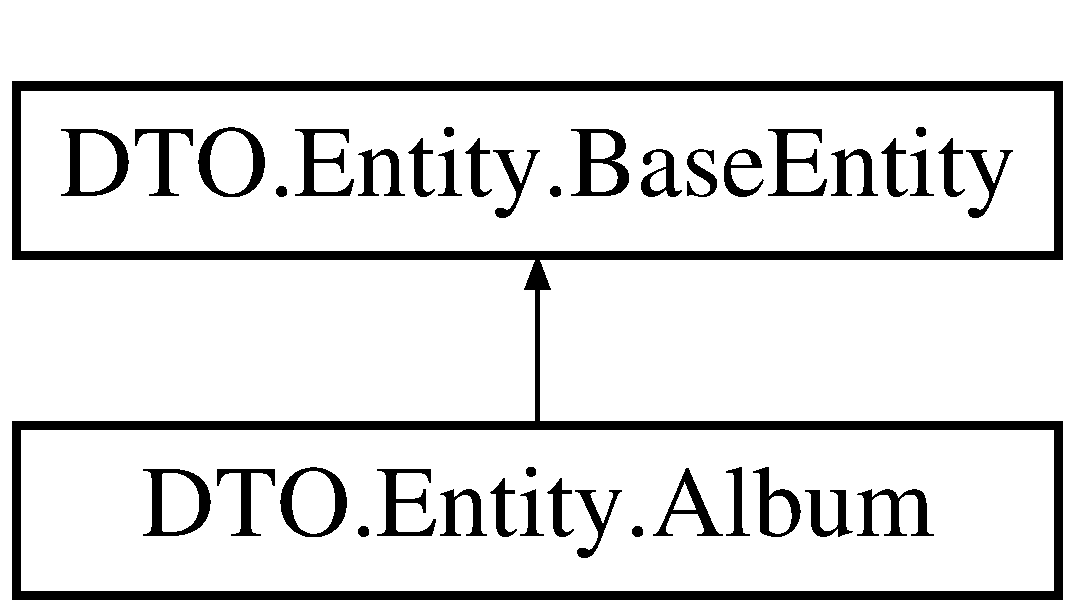
\includegraphics[height=2.000000cm]{class_d_t_o_1_1_entity_1_1_album}
\end{center}
\end{figure}
\subsection*{Public Attributes}
\begin{DoxyCompactItemize}
\item 
\mbox{\Hypertarget{class_d_t_o_1_1_entity_1_1_album_a6ee3fc6083829740b30a4d8061ffde6b}\label{class_d_t_o_1_1_entity_1_1_album_a6ee3fc6083829740b30a4d8061ffde6b}} 
Bitmap\+Image {\bfseries Picture} =$>$ Music\+File.\+Get\+Image(Tracks.\+First\+Or\+Default().Path, Picture\+Link)
\end{DoxyCompactItemize}
\subsection*{Properties}
\begin{DoxyCompactItemize}
\item 
\mbox{\Hypertarget{class_d_t_o_1_1_entity_1_1_album_a2e3b69ce750bfc558534a97f56f561af}\label{class_d_t_o_1_1_entity_1_1_album_a2e3b69ce750bfc558534a97f56f561af}} 
virtual \hyperlink{class_d_t_o_1_1_entity_1_1_artist}{Artist} {\bfseries Artist}\hspace{0.3cm}{\ttfamily  \mbox{[}get, set\mbox{]}}
\item 
\mbox{\Hypertarget{class_d_t_o_1_1_entity_1_1_album_a73f0921d2d0b9f5cf9c5052e6de73eb6}\label{class_d_t_o_1_1_entity_1_1_album_a73f0921d2d0b9f5cf9c5052e6de73eb6}} 
Date\+Time {\bfseries Date\+Creation}\hspace{0.3cm}{\ttfamily  \mbox{[}get, set\mbox{]}}
\item 
\mbox{\Hypertarget{class_d_t_o_1_1_entity_1_1_album_a803020baf473a40b224e7edf9c89b4e1}\label{class_d_t_o_1_1_entity_1_1_album_a803020baf473a40b224e7edf9c89b4e1}} 
long {\bfseries fk\+Artist}\hspace{0.3cm}{\ttfamily  \mbox{[}get, set\mbox{]}}
\item 
\mbox{\Hypertarget{class_d_t_o_1_1_entity_1_1_album_ab9b2ef7036e68ba646c80f81ffff62f1}\label{class_d_t_o_1_1_entity_1_1_album_ab9b2ef7036e68ba646c80f81ffff62f1}} 
string {\bfseries Name}\hspace{0.3cm}{\ttfamily  \mbox{[}get, set\mbox{]}}
\item 
\mbox{\Hypertarget{class_d_t_o_1_1_entity_1_1_album_acd55913e832e38bde01dbe6b6c53c387}\label{class_d_t_o_1_1_entity_1_1_album_acd55913e832e38bde01dbe6b6c53c387}} 
string {\bfseries Picture\+Link}\hspace{0.3cm}{\ttfamily  \mbox{[}get, set\mbox{]}}
\item 
\mbox{\Hypertarget{class_d_t_o_1_1_entity_1_1_album_a25b6b9b11765125899d7d3a05905d6b7}\label{class_d_t_o_1_1_entity_1_1_album_a25b6b9b11765125899d7d3a05905d6b7}} 
virtual I\+Collection$<$ \hyperlink{class_d_t_o_1_1_entity_1_1_track}{Track} $>$ {\bfseries Tracks}\hspace{0.3cm}{\ttfamily  \mbox{[}get, set\mbox{]}}
\end{DoxyCompactItemize}


\subsection{Detailed Description}
The database \hyperlink{class_d_t_o_1_1_entity_1_1_album}{Album} entity 



The documentation for this class was generated from the following file\+:\begin{DoxyCompactItemize}
\item 
C\+:/\+W\+O\+R\+K\+S\+P\+A\+C\+E/\+T\+P\+I-\/end/\+Gestion\+Audio/\+D\+T\+O/\+Entity/Album.\+cs\end{DoxyCompactItemize}

\hypertarget{class_presentation_1_1_view_1_1_list_1_1_album_list_view}{}\section{Presentation.\+View.\+List.\+Album\+List\+View Class Reference}
\label{class_presentation_1_1_view_1_1_list_1_1_album_list_view}\index{Presentation.\+View.\+List.\+Album\+List\+View@{Presentation.\+View.\+List.\+Album\+List\+View}}


\hyperlink{class_presentation_1_1_view_1_1_list_1_1_album_list_view}{Album\+List\+View}  


Inheritance diagram for Presentation.\+View.\+List.\+Album\+List\+View\+:\begin{figure}[H]
\begin{center}
\leavevmode
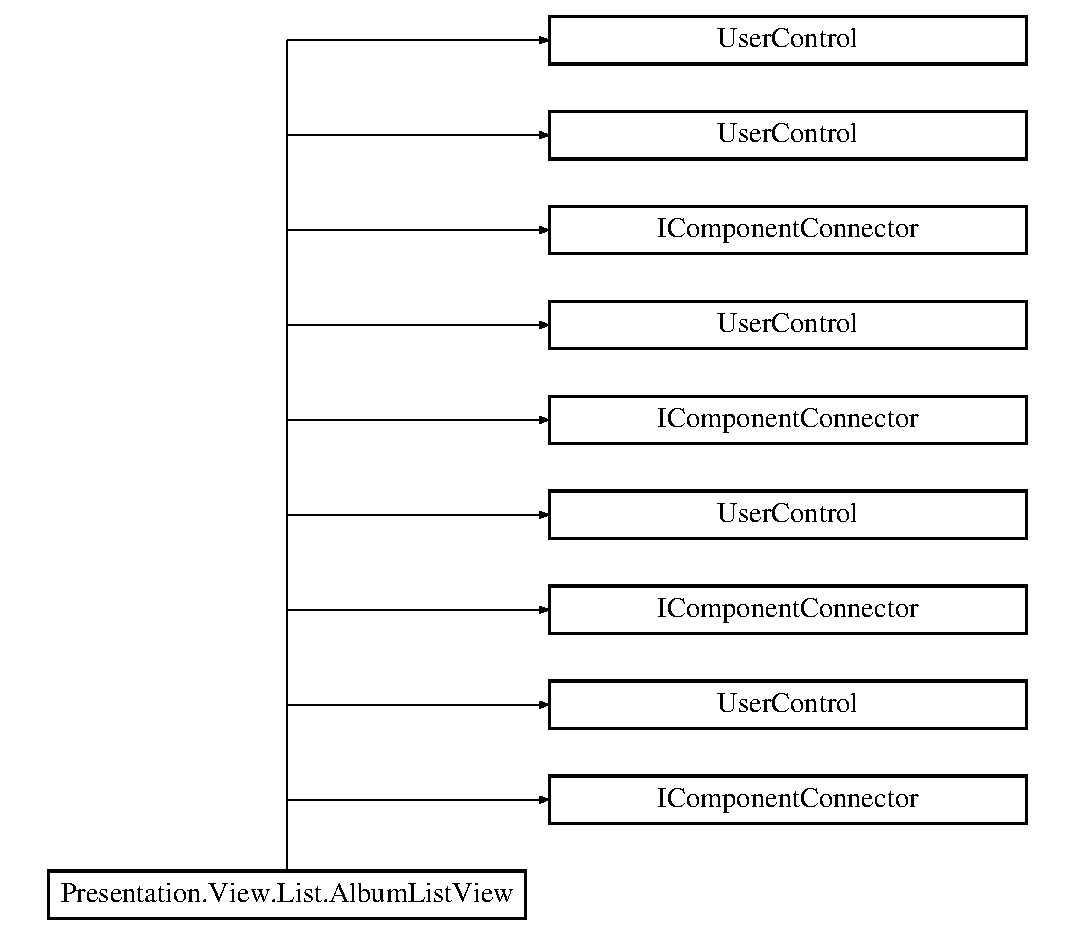
\includegraphics[height=10.000000cm]{class_presentation_1_1_view_1_1_list_1_1_album_list_view}
\end{center}
\end{figure}
\subsection*{Public Member Functions}
\begin{DoxyCompactItemize}
\item 
void \hyperlink{class_presentation_1_1_view_1_1_list_1_1_album_list_view_a82f7cb6e5ba3705196d1dcf9d1067b34}{Initialize\+Component} ()
\begin{DoxyCompactList}\small\item\em Initialize\+Component \end{DoxyCompactList}\item 
void \hyperlink{class_presentation_1_1_view_1_1_list_1_1_album_list_view_a82f7cb6e5ba3705196d1dcf9d1067b34}{Initialize\+Component} ()
\begin{DoxyCompactList}\small\item\em Initialize\+Component \end{DoxyCompactList}\item 
void \hyperlink{class_presentation_1_1_view_1_1_list_1_1_album_list_view_a82f7cb6e5ba3705196d1dcf9d1067b34}{Initialize\+Component} ()
\begin{DoxyCompactList}\small\item\em Initialize\+Component \end{DoxyCompactList}\item 
void \hyperlink{class_presentation_1_1_view_1_1_list_1_1_album_list_view_a82f7cb6e5ba3705196d1dcf9d1067b34}{Initialize\+Component} ()
\begin{DoxyCompactList}\small\item\em Initialize\+Component \end{DoxyCompactList}\end{DoxyCompactItemize}


\subsection{Detailed Description}
\hyperlink{class_presentation_1_1_view_1_1_list_1_1_album_list_view}{Album\+List\+View} 

Interaction logic for Music\+Home.\+xaml 

\subsection{Member Function Documentation}
\mbox{\Hypertarget{class_presentation_1_1_view_1_1_list_1_1_album_list_view_a82f7cb6e5ba3705196d1dcf9d1067b34}\label{class_presentation_1_1_view_1_1_list_1_1_album_list_view_a82f7cb6e5ba3705196d1dcf9d1067b34}} 
\index{Presentation\+::\+View\+::\+List\+::\+Album\+List\+View@{Presentation\+::\+View\+::\+List\+::\+Album\+List\+View}!Initialize\+Component@{Initialize\+Component}}
\index{Initialize\+Component@{Initialize\+Component}!Presentation\+::\+View\+::\+List\+::\+Album\+List\+View@{Presentation\+::\+View\+::\+List\+::\+Album\+List\+View}}
\subsubsection{\texorpdfstring{Initialize\+Component()}{InitializeComponent()}\hspace{0.1cm}{\footnotesize\ttfamily [1/4]}}
{\footnotesize\ttfamily void Presentation.\+View.\+List.\+Album\+List\+View.\+Initialize\+Component (\begin{DoxyParamCaption}{ }\end{DoxyParamCaption})}



Initialize\+Component 

\mbox{\Hypertarget{class_presentation_1_1_view_1_1_list_1_1_album_list_view_a82f7cb6e5ba3705196d1dcf9d1067b34}\label{class_presentation_1_1_view_1_1_list_1_1_album_list_view_a82f7cb6e5ba3705196d1dcf9d1067b34}} 
\index{Presentation\+::\+View\+::\+List\+::\+Album\+List\+View@{Presentation\+::\+View\+::\+List\+::\+Album\+List\+View}!Initialize\+Component@{Initialize\+Component}}
\index{Initialize\+Component@{Initialize\+Component}!Presentation\+::\+View\+::\+List\+::\+Album\+List\+View@{Presentation\+::\+View\+::\+List\+::\+Album\+List\+View}}
\subsubsection{\texorpdfstring{Initialize\+Component()}{InitializeComponent()}\hspace{0.1cm}{\footnotesize\ttfamily [2/4]}}
{\footnotesize\ttfamily void Presentation.\+View.\+List.\+Album\+List\+View.\+Initialize\+Component (\begin{DoxyParamCaption}{ }\end{DoxyParamCaption})}



Initialize\+Component 

\mbox{\Hypertarget{class_presentation_1_1_view_1_1_list_1_1_album_list_view_a82f7cb6e5ba3705196d1dcf9d1067b34}\label{class_presentation_1_1_view_1_1_list_1_1_album_list_view_a82f7cb6e5ba3705196d1dcf9d1067b34}} 
\index{Presentation\+::\+View\+::\+List\+::\+Album\+List\+View@{Presentation\+::\+View\+::\+List\+::\+Album\+List\+View}!Initialize\+Component@{Initialize\+Component}}
\index{Initialize\+Component@{Initialize\+Component}!Presentation\+::\+View\+::\+List\+::\+Album\+List\+View@{Presentation\+::\+View\+::\+List\+::\+Album\+List\+View}}
\subsubsection{\texorpdfstring{Initialize\+Component()}{InitializeComponent()}\hspace{0.1cm}{\footnotesize\ttfamily [3/4]}}
{\footnotesize\ttfamily void Presentation.\+View.\+List.\+Album\+List\+View.\+Initialize\+Component (\begin{DoxyParamCaption}{ }\end{DoxyParamCaption})}



Initialize\+Component 

\mbox{\Hypertarget{class_presentation_1_1_view_1_1_list_1_1_album_list_view_a82f7cb6e5ba3705196d1dcf9d1067b34}\label{class_presentation_1_1_view_1_1_list_1_1_album_list_view_a82f7cb6e5ba3705196d1dcf9d1067b34}} 
\index{Presentation\+::\+View\+::\+List\+::\+Album\+List\+View@{Presentation\+::\+View\+::\+List\+::\+Album\+List\+View}!Initialize\+Component@{Initialize\+Component}}
\index{Initialize\+Component@{Initialize\+Component}!Presentation\+::\+View\+::\+List\+::\+Album\+List\+View@{Presentation\+::\+View\+::\+List\+::\+Album\+List\+View}}
\subsubsection{\texorpdfstring{Initialize\+Component()}{InitializeComponent()}\hspace{0.1cm}{\footnotesize\ttfamily [4/4]}}
{\footnotesize\ttfamily void Presentation.\+View.\+List.\+Album\+List\+View.\+Initialize\+Component (\begin{DoxyParamCaption}{ }\end{DoxyParamCaption})}



Initialize\+Component 



The documentation for this class was generated from the following files\+:\begin{DoxyCompactItemize}
\item 
C\+:/\+W\+O\+R\+K\+S\+P\+A\+C\+E/\+T\+P\+I-\/end/\+Gestion\+Audio/\+Gestion\+Audio/obj/\+Debug/\+View/\+List/Album\+List\+View.\+g.\+cs\item 
C\+:/\+W\+O\+R\+K\+S\+P\+A\+C\+E/\+T\+P\+I-\/end/\+Gestion\+Audio/\+Gestion\+Audio/obj/\+Debug/\+View/\+List/Album\+List\+View.\+g.\+i.\+cs\item 
C\+:/\+W\+O\+R\+K\+S\+P\+A\+C\+E/\+T\+P\+I-\/end/\+Gestion\+Audio/\+Gestion\+Audio/\+View/\+List/Album\+List\+View.\+xaml.\+cs\end{DoxyCompactItemize}

\hypertarget{class_presentation_1_1_app}{}\section{Presentation.\+App Class Reference}
\label{class_presentation_1_1_app}\index{Presentation.\+App@{Presentation.\+App}}


Interaction logic for App.\+xaml  


Inheritance diagram for Presentation.\+App\+:\begin{figure}[H]
\begin{center}
\leavevmode
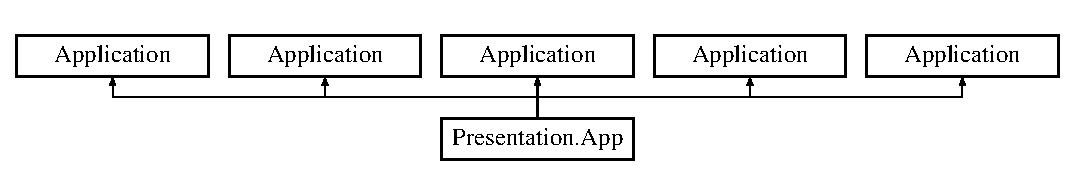
\includegraphics[height=1.914530cm]{class_presentation_1_1_app}
\end{center}
\end{figure}
\subsection*{Public Member Functions}
\begin{DoxyCompactItemize}
\item 
void \hyperlink{class_presentation_1_1_app_a7460ac4ca59a6b42035e0415cff24413}{Initialize\+Component} ()
\begin{DoxyCompactList}\small\item\em Initialize\+Component \end{DoxyCompactList}\item 
void \hyperlink{class_presentation_1_1_app_a7460ac4ca59a6b42035e0415cff24413}{Initialize\+Component} ()
\begin{DoxyCompactList}\small\item\em Initialize\+Component \end{DoxyCompactList}\item 
void \hyperlink{class_presentation_1_1_app_a7460ac4ca59a6b42035e0415cff24413}{Initialize\+Component} ()
\begin{DoxyCompactList}\small\item\em Initialize\+Component \end{DoxyCompactList}\item 
void \hyperlink{class_presentation_1_1_app_a7460ac4ca59a6b42035e0415cff24413}{Initialize\+Component} ()
\begin{DoxyCompactList}\small\item\em Initialize\+Component \end{DoxyCompactList}\end{DoxyCompactItemize}
\subsection*{Static Public Member Functions}
\begin{DoxyCompactItemize}
\item 
static void \hyperlink{class_presentation_1_1_app_a8a6ad434f351a99acb7059899b1f273c}{Main} ()
\begin{DoxyCompactList}\small\item\em Application Entry Point. \end{DoxyCompactList}\item 
static void \hyperlink{class_presentation_1_1_app_a8a6ad434f351a99acb7059899b1f273c}{Main} ()
\begin{DoxyCompactList}\small\item\em Application Entry Point. \end{DoxyCompactList}\item 
static void \hyperlink{class_presentation_1_1_app_a8a6ad434f351a99acb7059899b1f273c}{Main} ()
\begin{DoxyCompactList}\small\item\em Application Entry Point. \end{DoxyCompactList}\item 
static void \hyperlink{class_presentation_1_1_app_a8a6ad434f351a99acb7059899b1f273c}{Main} ()
\begin{DoxyCompactList}\small\item\em Application Entry Point. \end{DoxyCompactList}\end{DoxyCompactItemize}


\subsection{Detailed Description}
Interaction logic for App.\+xaml 

\hyperlink{class_presentation_1_1_app}{App} 

\subsection{Member Function Documentation}
\mbox{\Hypertarget{class_presentation_1_1_app_a7460ac4ca59a6b42035e0415cff24413}\label{class_presentation_1_1_app_a7460ac4ca59a6b42035e0415cff24413}} 
\index{Presentation\+::\+App@{Presentation\+::\+App}!Initialize\+Component@{Initialize\+Component}}
\index{Initialize\+Component@{Initialize\+Component}!Presentation\+::\+App@{Presentation\+::\+App}}
\subsubsection{\texorpdfstring{Initialize\+Component()}{InitializeComponent()}\hspace{0.1cm}{\footnotesize\ttfamily [1/4]}}
{\footnotesize\ttfamily void Presentation.\+App.\+Initialize\+Component (\begin{DoxyParamCaption}{ }\end{DoxyParamCaption})}



Initialize\+Component 

\mbox{\Hypertarget{class_presentation_1_1_app_a7460ac4ca59a6b42035e0415cff24413}\label{class_presentation_1_1_app_a7460ac4ca59a6b42035e0415cff24413}} 
\index{Presentation\+::\+App@{Presentation\+::\+App}!Initialize\+Component@{Initialize\+Component}}
\index{Initialize\+Component@{Initialize\+Component}!Presentation\+::\+App@{Presentation\+::\+App}}
\subsubsection{\texorpdfstring{Initialize\+Component()}{InitializeComponent()}\hspace{0.1cm}{\footnotesize\ttfamily [2/4]}}
{\footnotesize\ttfamily void Presentation.\+App.\+Initialize\+Component (\begin{DoxyParamCaption}{ }\end{DoxyParamCaption})}



Initialize\+Component 

\mbox{\Hypertarget{class_presentation_1_1_app_a7460ac4ca59a6b42035e0415cff24413}\label{class_presentation_1_1_app_a7460ac4ca59a6b42035e0415cff24413}} 
\index{Presentation\+::\+App@{Presentation\+::\+App}!Initialize\+Component@{Initialize\+Component}}
\index{Initialize\+Component@{Initialize\+Component}!Presentation\+::\+App@{Presentation\+::\+App}}
\subsubsection{\texorpdfstring{Initialize\+Component()}{InitializeComponent()}\hspace{0.1cm}{\footnotesize\ttfamily [3/4]}}
{\footnotesize\ttfamily void Presentation.\+App.\+Initialize\+Component (\begin{DoxyParamCaption}{ }\end{DoxyParamCaption})}



Initialize\+Component 

\mbox{\Hypertarget{class_presentation_1_1_app_a7460ac4ca59a6b42035e0415cff24413}\label{class_presentation_1_1_app_a7460ac4ca59a6b42035e0415cff24413}} 
\index{Presentation\+::\+App@{Presentation\+::\+App}!Initialize\+Component@{Initialize\+Component}}
\index{Initialize\+Component@{Initialize\+Component}!Presentation\+::\+App@{Presentation\+::\+App}}
\subsubsection{\texorpdfstring{Initialize\+Component()}{InitializeComponent()}\hspace{0.1cm}{\footnotesize\ttfamily [4/4]}}
{\footnotesize\ttfamily void Presentation.\+App.\+Initialize\+Component (\begin{DoxyParamCaption}{ }\end{DoxyParamCaption})}



Initialize\+Component 

\mbox{\Hypertarget{class_presentation_1_1_app_a8a6ad434f351a99acb7059899b1f273c}\label{class_presentation_1_1_app_a8a6ad434f351a99acb7059899b1f273c}} 
\index{Presentation\+::\+App@{Presentation\+::\+App}!Main@{Main}}
\index{Main@{Main}!Presentation\+::\+App@{Presentation\+::\+App}}
\subsubsection{\texorpdfstring{Main()}{Main()}\hspace{0.1cm}{\footnotesize\ttfamily [1/4]}}
{\footnotesize\ttfamily static void Presentation.\+App.\+Main (\begin{DoxyParamCaption}{ }\end{DoxyParamCaption})\hspace{0.3cm}{\ttfamily [static]}}



Application Entry Point. 

\mbox{\Hypertarget{class_presentation_1_1_app_a8a6ad434f351a99acb7059899b1f273c}\label{class_presentation_1_1_app_a8a6ad434f351a99acb7059899b1f273c}} 
\index{Presentation\+::\+App@{Presentation\+::\+App}!Main@{Main}}
\index{Main@{Main}!Presentation\+::\+App@{Presentation\+::\+App}}
\subsubsection{\texorpdfstring{Main()}{Main()}\hspace{0.1cm}{\footnotesize\ttfamily [2/4]}}
{\footnotesize\ttfamily static void Presentation.\+App.\+Main (\begin{DoxyParamCaption}{ }\end{DoxyParamCaption})\hspace{0.3cm}{\ttfamily [static]}}



Application Entry Point. 

\mbox{\Hypertarget{class_presentation_1_1_app_a8a6ad434f351a99acb7059899b1f273c}\label{class_presentation_1_1_app_a8a6ad434f351a99acb7059899b1f273c}} 
\index{Presentation\+::\+App@{Presentation\+::\+App}!Main@{Main}}
\index{Main@{Main}!Presentation\+::\+App@{Presentation\+::\+App}}
\subsubsection{\texorpdfstring{Main()}{Main()}\hspace{0.1cm}{\footnotesize\ttfamily [3/4]}}
{\footnotesize\ttfamily static void Presentation.\+App.\+Main (\begin{DoxyParamCaption}{ }\end{DoxyParamCaption})\hspace{0.3cm}{\ttfamily [static]}}



Application Entry Point. 

\mbox{\Hypertarget{class_presentation_1_1_app_a8a6ad434f351a99acb7059899b1f273c}\label{class_presentation_1_1_app_a8a6ad434f351a99acb7059899b1f273c}} 
\index{Presentation\+::\+App@{Presentation\+::\+App}!Main@{Main}}
\index{Main@{Main}!Presentation\+::\+App@{Presentation\+::\+App}}
\subsubsection{\texorpdfstring{Main()}{Main()}\hspace{0.1cm}{\footnotesize\ttfamily [4/4]}}
{\footnotesize\ttfamily static void Presentation.\+App.\+Main (\begin{DoxyParamCaption}{ }\end{DoxyParamCaption})\hspace{0.3cm}{\ttfamily [static]}}



Application Entry Point. 



The documentation for this class was generated from the following files\+:\begin{DoxyCompactItemize}
\item 
C\+:/\+W\+O\+R\+K\+S\+P\+A\+C\+E/\+T\+P\+I-\/end/\+Gestion\+Audio/\+Gestion\+Audio/App.\+xaml.\+cs\item 
C\+:/\+W\+O\+R\+K\+S\+P\+A\+C\+E/\+T\+P\+I-\/end/\+Gestion\+Audio/\+Gestion\+Audio/obj/\+Debug/App.\+g.\+cs\item 
C\+:/\+W\+O\+R\+K\+S\+P\+A\+C\+E/\+T\+P\+I-\/end/\+Gestion\+Audio/\+Gestion\+Audio/obj/\+Debug/App.\+g.\+i.\+cs\end{DoxyCompactItemize}

\hypertarget{class_d_t_o_1_1_entity_1_1_artist}{}\section{D\+T\+O.\+Entity.\+Artist Class Reference}
\label{class_d_t_o_1_1_entity_1_1_artist}\index{D\+T\+O.\+Entity.\+Artist@{D\+T\+O.\+Entity.\+Artist}}


The database \hyperlink{class_d_t_o_1_1_entity_1_1_artist}{Artist} entity  


Inheritance diagram for D\+T\+O.\+Entity.\+Artist\+:\begin{figure}[H]
\begin{center}
\leavevmode
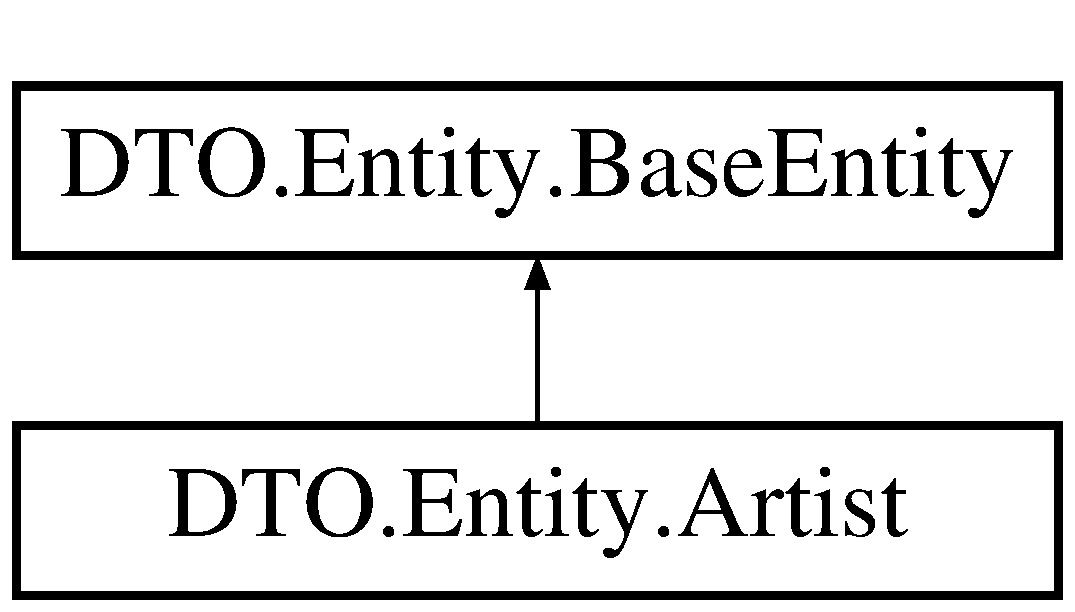
\includegraphics[height=2.000000cm]{class_d_t_o_1_1_entity_1_1_artist}
\end{center}
\end{figure}
\subsection*{Properties}
\begin{DoxyCompactItemize}
\item 
\mbox{\Hypertarget{class_d_t_o_1_1_entity_1_1_artist_a1bc514b69f4031bc7be26a11afac7ce2}\label{class_d_t_o_1_1_entity_1_1_artist_a1bc514b69f4031bc7be26a11afac7ce2}} 
virtual I\+Collection$<$ \hyperlink{class_d_t_o_1_1_entity_1_1_album}{Album} $>$ {\bfseries Albums}\hspace{0.3cm}{\ttfamily  \mbox{[}get, set\mbox{]}}
\item 
\mbox{\Hypertarget{class_d_t_o_1_1_entity_1_1_artist_a57376a1185e8c279676df7271686d59f}\label{class_d_t_o_1_1_entity_1_1_artist_a57376a1185e8c279676df7271686d59f}} 
string {\bfseries Name}\hspace{0.3cm}{\ttfamily  \mbox{[}get, set\mbox{]}}
\end{DoxyCompactItemize}


\subsection{Detailed Description}
The database \hyperlink{class_d_t_o_1_1_entity_1_1_artist}{Artist} entity 



The documentation for this class was generated from the following file\+:\begin{DoxyCompactItemize}
\item 
C\+:/\+W\+O\+R\+K\+S\+P\+A\+C\+E/\+T\+P\+I-\/end/\+Gestion\+Audio/\+D\+T\+O/\+Entity/Artist.\+cs\end{DoxyCompactItemize}

\hypertarget{class_presentation_1_1_view_1_1_list_1_1_artist_list_view}{}\section{Presentation.\+View.\+List.\+Artist\+List\+View Class Reference}
\label{class_presentation_1_1_view_1_1_list_1_1_artist_list_view}\index{Presentation.\+View.\+List.\+Artist\+List\+View@{Presentation.\+View.\+List.\+Artist\+List\+View}}


\hyperlink{class_presentation_1_1_view_1_1_list_1_1_artist_list_view}{Artist\+List\+View}  


Inheritance diagram for Presentation.\+View.\+List.\+Artist\+List\+View\+:\begin{figure}[H]
\begin{center}
\leavevmode
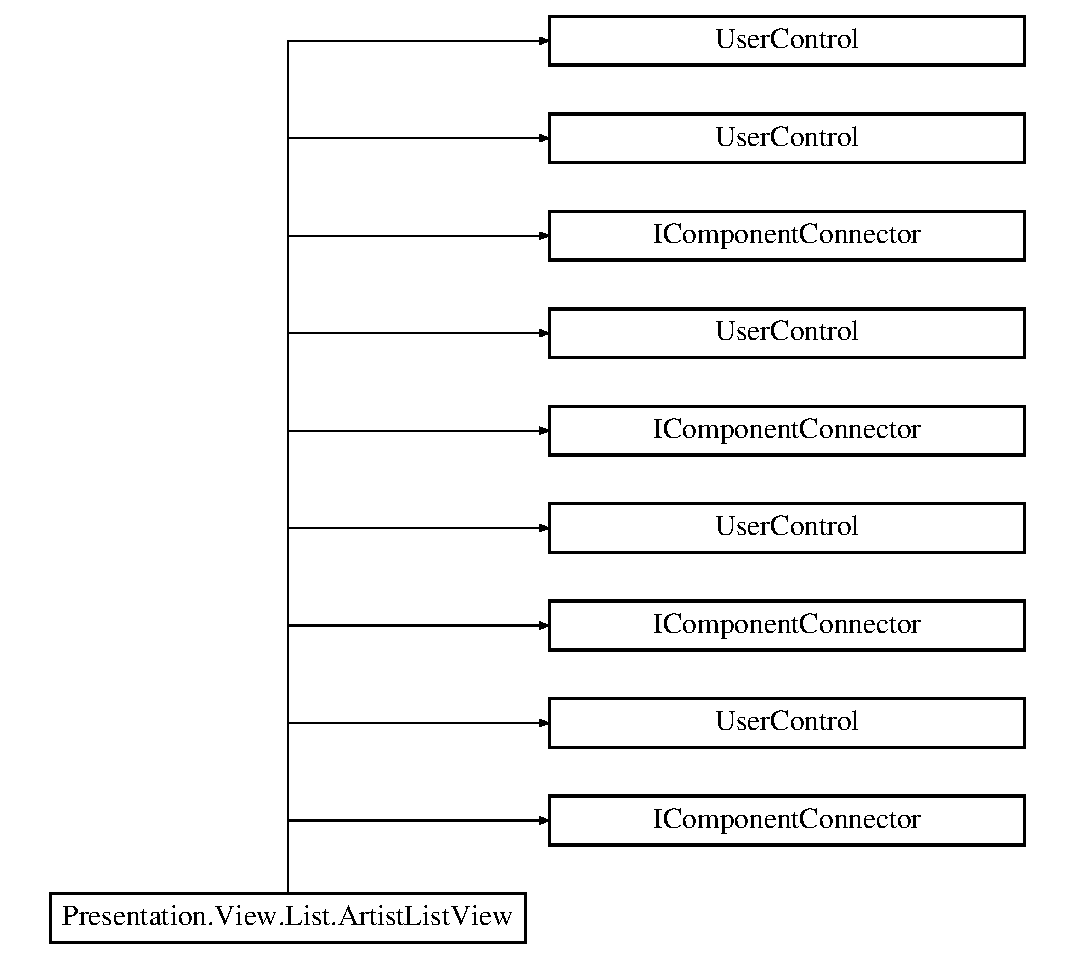
\includegraphics[height=10.000000cm]{class_presentation_1_1_view_1_1_list_1_1_artist_list_view}
\end{center}
\end{figure}
\subsection*{Public Member Functions}
\begin{DoxyCompactItemize}
\item 
void \hyperlink{class_presentation_1_1_view_1_1_list_1_1_artist_list_view_a64ae6fa24884ea06d766083a1576dc4d}{Initialize\+Component} ()
\begin{DoxyCompactList}\small\item\em Initialize\+Component \end{DoxyCompactList}\item 
void \hyperlink{class_presentation_1_1_view_1_1_list_1_1_artist_list_view_a64ae6fa24884ea06d766083a1576dc4d}{Initialize\+Component} ()
\begin{DoxyCompactList}\small\item\em Initialize\+Component \end{DoxyCompactList}\item 
void \hyperlink{class_presentation_1_1_view_1_1_list_1_1_artist_list_view_a64ae6fa24884ea06d766083a1576dc4d}{Initialize\+Component} ()
\begin{DoxyCompactList}\small\item\em Initialize\+Component \end{DoxyCompactList}\item 
void \hyperlink{class_presentation_1_1_view_1_1_list_1_1_artist_list_view_a64ae6fa24884ea06d766083a1576dc4d}{Initialize\+Component} ()
\begin{DoxyCompactList}\small\item\em Initialize\+Component \end{DoxyCompactList}\end{DoxyCompactItemize}


\subsection{Detailed Description}
\hyperlink{class_presentation_1_1_view_1_1_list_1_1_artist_list_view}{Artist\+List\+View} 

Interaction logic for Music\+Home.\+xaml 

\subsection{Member Function Documentation}
\mbox{\Hypertarget{class_presentation_1_1_view_1_1_list_1_1_artist_list_view_a64ae6fa24884ea06d766083a1576dc4d}\label{class_presentation_1_1_view_1_1_list_1_1_artist_list_view_a64ae6fa24884ea06d766083a1576dc4d}} 
\index{Presentation\+::\+View\+::\+List\+::\+Artist\+List\+View@{Presentation\+::\+View\+::\+List\+::\+Artist\+List\+View}!Initialize\+Component@{Initialize\+Component}}
\index{Initialize\+Component@{Initialize\+Component}!Presentation\+::\+View\+::\+List\+::\+Artist\+List\+View@{Presentation\+::\+View\+::\+List\+::\+Artist\+List\+View}}
\subsubsection{\texorpdfstring{Initialize\+Component()}{InitializeComponent()}\hspace{0.1cm}{\footnotesize\ttfamily [1/4]}}
{\footnotesize\ttfamily void Presentation.\+View.\+List.\+Artist\+List\+View.\+Initialize\+Component (\begin{DoxyParamCaption}{ }\end{DoxyParamCaption})}



Initialize\+Component 

\mbox{\Hypertarget{class_presentation_1_1_view_1_1_list_1_1_artist_list_view_a64ae6fa24884ea06d766083a1576dc4d}\label{class_presentation_1_1_view_1_1_list_1_1_artist_list_view_a64ae6fa24884ea06d766083a1576dc4d}} 
\index{Presentation\+::\+View\+::\+List\+::\+Artist\+List\+View@{Presentation\+::\+View\+::\+List\+::\+Artist\+List\+View}!Initialize\+Component@{Initialize\+Component}}
\index{Initialize\+Component@{Initialize\+Component}!Presentation\+::\+View\+::\+List\+::\+Artist\+List\+View@{Presentation\+::\+View\+::\+List\+::\+Artist\+List\+View}}
\subsubsection{\texorpdfstring{Initialize\+Component()}{InitializeComponent()}\hspace{0.1cm}{\footnotesize\ttfamily [2/4]}}
{\footnotesize\ttfamily void Presentation.\+View.\+List.\+Artist\+List\+View.\+Initialize\+Component (\begin{DoxyParamCaption}{ }\end{DoxyParamCaption})}



Initialize\+Component 

\mbox{\Hypertarget{class_presentation_1_1_view_1_1_list_1_1_artist_list_view_a64ae6fa24884ea06d766083a1576dc4d}\label{class_presentation_1_1_view_1_1_list_1_1_artist_list_view_a64ae6fa24884ea06d766083a1576dc4d}} 
\index{Presentation\+::\+View\+::\+List\+::\+Artist\+List\+View@{Presentation\+::\+View\+::\+List\+::\+Artist\+List\+View}!Initialize\+Component@{Initialize\+Component}}
\index{Initialize\+Component@{Initialize\+Component}!Presentation\+::\+View\+::\+List\+::\+Artist\+List\+View@{Presentation\+::\+View\+::\+List\+::\+Artist\+List\+View}}
\subsubsection{\texorpdfstring{Initialize\+Component()}{InitializeComponent()}\hspace{0.1cm}{\footnotesize\ttfamily [3/4]}}
{\footnotesize\ttfamily void Presentation.\+View.\+List.\+Artist\+List\+View.\+Initialize\+Component (\begin{DoxyParamCaption}{ }\end{DoxyParamCaption})}



Initialize\+Component 

\mbox{\Hypertarget{class_presentation_1_1_view_1_1_list_1_1_artist_list_view_a64ae6fa24884ea06d766083a1576dc4d}\label{class_presentation_1_1_view_1_1_list_1_1_artist_list_view_a64ae6fa24884ea06d766083a1576dc4d}} 
\index{Presentation\+::\+View\+::\+List\+::\+Artist\+List\+View@{Presentation\+::\+View\+::\+List\+::\+Artist\+List\+View}!Initialize\+Component@{Initialize\+Component}}
\index{Initialize\+Component@{Initialize\+Component}!Presentation\+::\+View\+::\+List\+::\+Artist\+List\+View@{Presentation\+::\+View\+::\+List\+::\+Artist\+List\+View}}
\subsubsection{\texorpdfstring{Initialize\+Component()}{InitializeComponent()}\hspace{0.1cm}{\footnotesize\ttfamily [4/4]}}
{\footnotesize\ttfamily void Presentation.\+View.\+List.\+Artist\+List\+View.\+Initialize\+Component (\begin{DoxyParamCaption}{ }\end{DoxyParamCaption})}



Initialize\+Component 



The documentation for this class was generated from the following files\+:\begin{DoxyCompactItemize}
\item 
C\+:/\+W\+O\+R\+K\+S\+P\+A\+C\+E/\+T\+P\+I-\/end/\+Gestion\+Audio/\+Gestion\+Audio/obj/\+Debug/\+View/\+List/Artist\+List\+View.\+g.\+cs\item 
C\+:/\+W\+O\+R\+K\+S\+P\+A\+C\+E/\+T\+P\+I-\/end/\+Gestion\+Audio/\+Gestion\+Audio/obj/\+Debug/\+View/\+List/Artist\+List\+View.\+g.\+i.\+cs\item 
C\+:/\+W\+O\+R\+K\+S\+P\+A\+C\+E/\+T\+P\+I-\/end/\+Gestion\+Audio/\+Gestion\+Audio/\+View/\+List/Artist\+List\+View.\+xaml.\+cs\end{DoxyCompactItemize}

\hypertarget{class_d_t_o_1_1_audio}{}\section{D\+T\+O.\+Audio Class Reference}
\label{class_d_t_o_1_1_audio}\index{D\+T\+O.\+Audio@{D\+T\+O.\+Audio}}


The link between radio and track  


Inheritance diagram for D\+T\+O.\+Audio\+:\begin{figure}[H]
\begin{center}
\leavevmode
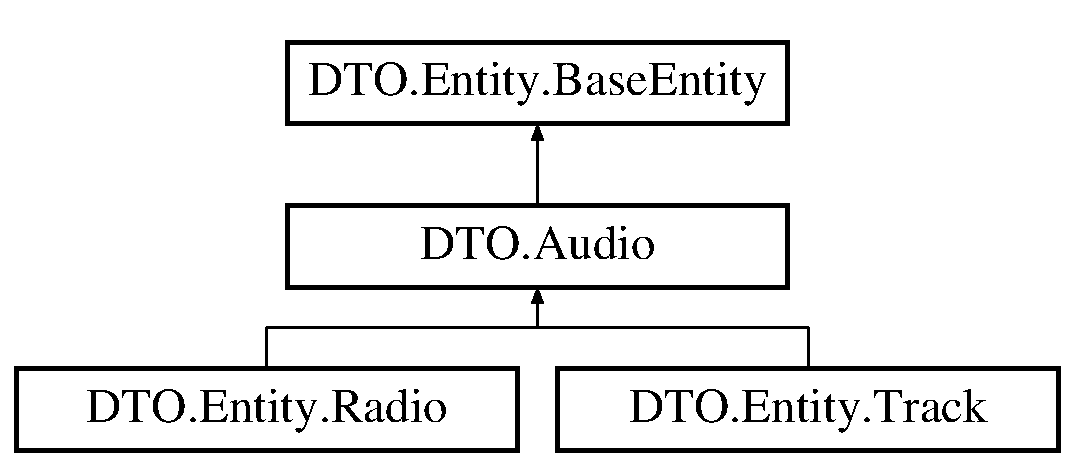
\includegraphics[height=3.000000cm]{class_d_t_o_1_1_audio}
\end{center}
\end{figure}
\subsection*{Public Attributes}
\begin{DoxyCompactItemize}
\item 
\mbox{\Hypertarget{class_d_t_o_1_1_audio_a5f75b29b3d11be9b911f68cec3977609}\label{class_d_t_o_1_1_audio_a5f75b29b3d11be9b911f68cec3977609}} 
string {\bfseries Genres\+String} =$>$ string.\+Join(\char`\"{}, \char`\"{}, Genres.\+Select(a =$>$ a.\+Name))
\item 
\mbox{\Hypertarget{class_d_t_o_1_1_audio_aaf2c66c9254f4ced7b106ae23184d85c}\label{class_d_t_o_1_1_audio_aaf2c66c9254f4ced7b106ae23184d85c}} 
Bitmap\+Image {\bfseries Picture} =$>$ this is \hyperlink{class_d_t_o_1_1_entity_1_1_radio}{Radio} ? new Bitmap\+Image(new Uri((this as \hyperlink{class_d_t_o_1_1_entity_1_1_radio}{Radio}).Logo\+Url)) \+: (this as \hyperlink{class_d_t_o_1_1_entity_1_1_track}{Track}).Album.\+Picture
\end{DoxyCompactItemize}
\subsection*{Properties}
\begin{DoxyCompactItemize}
\item 
\mbox{\Hypertarget{class_d_t_o_1_1_audio_a796dba75af345fa61826412a15b4f199}\label{class_d_t_o_1_1_audio_a796dba75af345fa61826412a15b4f199}} 
Wave\+Stream {\bfseries File}\hspace{0.3cm}{\ttfamily  \mbox{[}get, set\mbox{]}}
\item 
\mbox{\Hypertarget{class_d_t_o_1_1_audio_a64baf5725332a6021eb88a2756f0f445}\label{class_d_t_o_1_1_audio_a64baf5725332a6021eb88a2756f0f445}} 
virtual List$<$ \hyperlink{class_d_t_o_1_1_entity_1_1_genre}{Genre} $>$ {\bfseries Genres}\hspace{0.3cm}{\ttfamily  \mbox{[}get, set\mbox{]}}
\item 
\mbox{\Hypertarget{class_d_t_o_1_1_audio_acdff662b62eb37a7fe3f7950b9131c3b}\label{class_d_t_o_1_1_audio_acdff662b62eb37a7fe3f7950b9131c3b}} 
bool {\bfseries Is\+Favorite}\hspace{0.3cm}{\ttfamily  \mbox{[}get, set\mbox{]}}
\item 
\mbox{\Hypertarget{class_d_t_o_1_1_audio_acdcc82963e4ab0fef866fa1776023d02}\label{class_d_t_o_1_1_audio_acdcc82963e4ab0fef866fa1776023d02}} 
string {\bfseries Name}\hspace{0.3cm}{\ttfamily  \mbox{[}get, set\mbox{]}}
\item 
\mbox{\Hypertarget{class_d_t_o_1_1_audio_a0a8ec6ad3b10d7fd6adf59798b2f2d3a}\label{class_d_t_o_1_1_audio_a0a8ec6ad3b10d7fd6adf59798b2f2d3a}} 
string {\bfseries Path}\hspace{0.3cm}{\ttfamily  \mbox{[}get, set\mbox{]}}
\end{DoxyCompactItemize}


\subsection{Detailed Description}
The link between radio and track 



The documentation for this class was generated from the following file\+:\begin{DoxyCompactItemize}
\item 
C\+:/\+W\+O\+R\+K\+S\+P\+A\+C\+E/\+T\+P\+I-\/end/\+Gestion\+Audio/\+D\+T\+O/Audio.\+cs\end{DoxyCompactItemize}

\hypertarget{class_unit_test_1_1_audio_test}{}\section{Unit\+Test.\+Audio\+Test Class Reference}
\label{class_unit_test_1_1_audio_test}\index{Unit\+Test.\+Audio\+Test@{Unit\+Test.\+Audio\+Test}}


Contain all test to make a simple try work  


\subsection*{Public Member Functions}
\begin{DoxyCompactItemize}
\item 
void \hyperlink{class_unit_test_1_1_audio_test_a94e4251cb6c610e3cc7e4db515060a0c}{Check\+Track\+Info} ()
\begin{DoxyCompactList}\small\item\em Check that the track info I save is the same from the mp3 \end{DoxyCompactList}\item 
void \hyperlink{class_unit_test_1_1_audio_test_a6f1473adeea374f0d01e0c78bbfe4c02}{Create\+Playlist} ()
\begin{DoxyCompactList}\small\item\em Create and add tracks to a playlist \end{DoxyCompactList}\item 
void \hyperlink{class_unit_test_1_1_audio_test_a8991e38cfa40fab3ae4b2ae355ac2738}{Load\+Data} ()
\begin{DoxyCompactList}\small\item\em Create basic music datas \end{DoxyCompactList}\end{DoxyCompactItemize}


\subsection{Detailed Description}
Contain all test to make a simple try work 



\subsection{Member Function Documentation}
\mbox{\Hypertarget{class_unit_test_1_1_audio_test_a94e4251cb6c610e3cc7e4db515060a0c}\label{class_unit_test_1_1_audio_test_a94e4251cb6c610e3cc7e4db515060a0c}} 
\index{Unit\+Test\+::\+Audio\+Test@{Unit\+Test\+::\+Audio\+Test}!Check\+Track\+Info@{Check\+Track\+Info}}
\index{Check\+Track\+Info@{Check\+Track\+Info}!Unit\+Test\+::\+Audio\+Test@{Unit\+Test\+::\+Audio\+Test}}
\subsubsection{\texorpdfstring{Check\+Track\+Info()}{CheckTrackInfo()}}
{\footnotesize\ttfamily void Unit\+Test.\+Audio\+Test.\+Check\+Track\+Info (\begin{DoxyParamCaption}{ }\end{DoxyParamCaption})}



Check that the track info I save is the same from the mp3 

\mbox{\Hypertarget{class_unit_test_1_1_audio_test_a6f1473adeea374f0d01e0c78bbfe4c02}\label{class_unit_test_1_1_audio_test_a6f1473adeea374f0d01e0c78bbfe4c02}} 
\index{Unit\+Test\+::\+Audio\+Test@{Unit\+Test\+::\+Audio\+Test}!Create\+Playlist@{Create\+Playlist}}
\index{Create\+Playlist@{Create\+Playlist}!Unit\+Test\+::\+Audio\+Test@{Unit\+Test\+::\+Audio\+Test}}
\subsubsection{\texorpdfstring{Create\+Playlist()}{CreatePlaylist()}}
{\footnotesize\ttfamily void Unit\+Test.\+Audio\+Test.\+Create\+Playlist (\begin{DoxyParamCaption}{ }\end{DoxyParamCaption})}



Create and add tracks to a playlist 

\mbox{\Hypertarget{class_unit_test_1_1_audio_test_a8991e38cfa40fab3ae4b2ae355ac2738}\label{class_unit_test_1_1_audio_test_a8991e38cfa40fab3ae4b2ae355ac2738}} 
\index{Unit\+Test\+::\+Audio\+Test@{Unit\+Test\+::\+Audio\+Test}!Load\+Data@{Load\+Data}}
\index{Load\+Data@{Load\+Data}!Unit\+Test\+::\+Audio\+Test@{Unit\+Test\+::\+Audio\+Test}}
\subsubsection{\texorpdfstring{Load\+Data()}{LoadData()}}
{\footnotesize\ttfamily void Unit\+Test.\+Audio\+Test.\+Load\+Data (\begin{DoxyParamCaption}{ }\end{DoxyParamCaption})}



Create basic music datas 



The documentation for this class was generated from the following file\+:\begin{DoxyCompactItemize}
\item 
C\+:/\+W\+O\+R\+K\+S\+P\+A\+C\+E/\+T\+P\+I-\/end/\+Gestion\+Audio/\+Unit\+Test/Audio\+Test.\+cs\end{DoxyCompactItemize}

\hypertarget{class_d_t_o_1_1_entity_1_1_base_entity}{}\section{D\+T\+O.\+Entity.\+Base\+Entity Class Reference}
\label{class_d_t_o_1_1_entity_1_1_base_entity}\index{D\+T\+O.\+Entity.\+Base\+Entity@{D\+T\+O.\+Entity.\+Base\+Entity}}


The base entity, shared by all entities  


Inheritance diagram for D\+T\+O.\+Entity.\+Base\+Entity\+:\begin{figure}[H]
\begin{center}
\leavevmode
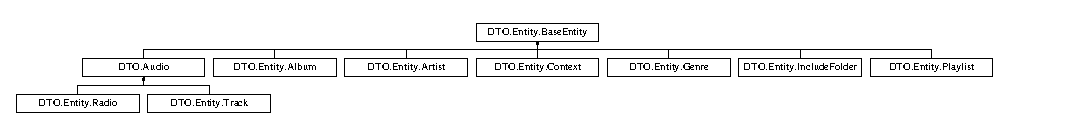
\includegraphics[height=1.288344cm]{class_d_t_o_1_1_entity_1_1_base_entity}
\end{center}
\end{figure}
\subsection*{Properties}
\begin{DoxyCompactItemize}
\item 
\mbox{\Hypertarget{class_d_t_o_1_1_entity_1_1_base_entity_a1186e3cdf350f3d532425c67d786e889}\label{class_d_t_o_1_1_entity_1_1_base_entity_a1186e3cdf350f3d532425c67d786e889}} 
long {\bfseries ID}\hspace{0.3cm}{\ttfamily  \mbox{[}get, set\mbox{]}}
\end{DoxyCompactItemize}


\subsection{Detailed Description}
The base entity, shared by all entities 



The documentation for this class was generated from the following file\+:\begin{DoxyCompactItemize}
\item 
C\+:/\+W\+O\+R\+K\+S\+P\+A\+C\+E/\+T\+P\+I-\/end/\+Gestion\+Audio/\+D\+T\+O/\+Entity/Base\+Entity.\+cs\end{DoxyCompactItemize}

\hypertarget{class_d_a_l_1_1_database_1_1_configuration}{}\section{D\+A\+L.\+Database.\+Configuration Class Reference}
\label{class_d_a_l_1_1_database_1_1_configuration}\index{D\+A\+L.\+Database.\+Configuration@{D\+A\+L.\+Database.\+Configuration}}


Set the configuration of the database (not for sqlite)  


Inheritance diagram for D\+A\+L.\+Database.\+Configuration\+:\begin{figure}[H]
\begin{center}
\leavevmode
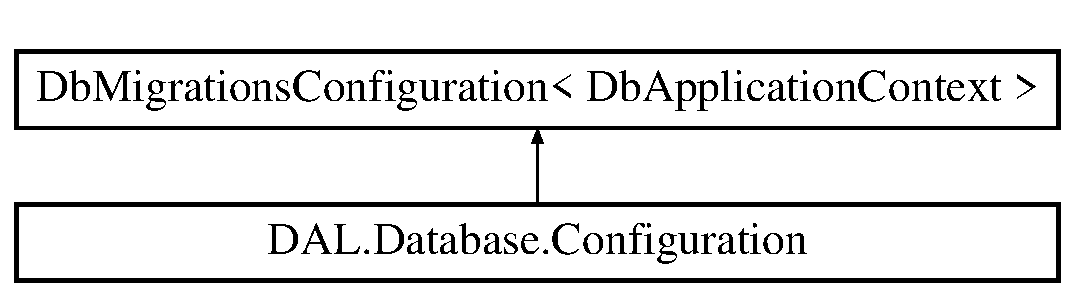
\includegraphics[height=2.000000cm]{class_d_a_l_1_1_database_1_1_configuration}
\end{center}
\end{figure}
\subsection*{Protected Member Functions}
\begin{DoxyCompactItemize}
\item 
override void \hyperlink{class_d_a_l_1_1_database_1_1_configuration_ab87c8987e23169c676d348d7433aaf21}{Seed} (\hyperlink{class_d_a_l_1_1_database_1_1_db_application_context}{Db\+Application\+Context} context)
\begin{DoxyCompactList}\small\item\em Populate the database \end{DoxyCompactList}\end{DoxyCompactItemize}


\subsection{Detailed Description}
Set the configuration of the database (not for sqlite) 



\subsection{Member Function Documentation}
\mbox{\Hypertarget{class_d_a_l_1_1_database_1_1_configuration_ab87c8987e23169c676d348d7433aaf21}\label{class_d_a_l_1_1_database_1_1_configuration_ab87c8987e23169c676d348d7433aaf21}} 
\index{D\+A\+L\+::\+Database\+::\+Configuration@{D\+A\+L\+::\+Database\+::\+Configuration}!Seed@{Seed}}
\index{Seed@{Seed}!D\+A\+L\+::\+Database\+::\+Configuration@{D\+A\+L\+::\+Database\+::\+Configuration}}
\subsubsection{\texorpdfstring{Seed()}{Seed()}}
{\footnotesize\ttfamily override void D\+A\+L.\+Database.\+Configuration.\+Seed (\begin{DoxyParamCaption}\item[{\hyperlink{class_d_a_l_1_1_database_1_1_db_application_context}{Db\+Application\+Context}}]{context }\end{DoxyParamCaption})\hspace{0.3cm}{\ttfamily [protected]}}



Populate the database 


\begin{DoxyParams}{Parameters}
{\em context} & \\
\hline
\end{DoxyParams}


The documentation for this class was generated from the following file\+:\begin{DoxyCompactItemize}
\item 
C\+:/\+W\+O\+R\+K\+S\+P\+A\+C\+E/\+T\+P\+I-\/end/\+Gestion\+Audio/\+D\+A\+L/\+Database/Configuration.\+cs\end{DoxyCompactItemize}

\hypertarget{class_d_t_o_1_1_entity_1_1_context}{}\section{D\+T\+O.\+Entity.\+Context Class Reference}
\label{class_d_t_o_1_1_entity_1_1_context}\index{D\+T\+O.\+Entity.\+Context@{D\+T\+O.\+Entity.\+Context}}


The database \hyperlink{class_d_t_o_1_1_entity_1_1_context}{Context} entity  


Inheritance diagram for D\+T\+O.\+Entity.\+Context\+:\begin{figure}[H]
\begin{center}
\leavevmode
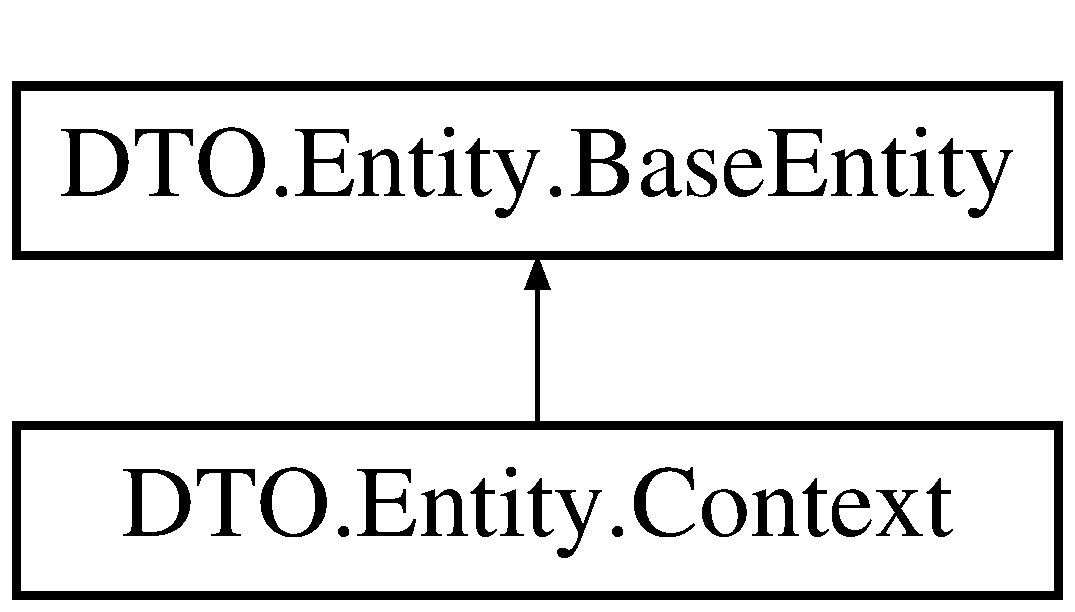
\includegraphics[height=2.000000cm]{class_d_t_o_1_1_entity_1_1_context}
\end{center}
\end{figure}
\subsection*{Public Attributes}
\begin{DoxyCompactItemize}
\item 
\mbox{\Hypertarget{class_d_t_o_1_1_entity_1_1_context_a5af319765cdba2ee3b63826ddcf77925}\label{class_d_t_o_1_1_entity_1_1_context_a5af319765cdba2ee3b63826ddcf77925}} 
\hyperlink{class_d_t_o_1_1_audio}{Audio} {\bfseries Actual\+Audio} =$>$ \hyperlink{class_d_t_o_1_1_entity_1_1_track}{Track} ?? (\hyperlink{class_d_t_o_1_1_audio}{Audio})\hyperlink{class_d_t_o_1_1_entity_1_1_radio}{Radio}
\end{DoxyCompactItemize}
\subsection*{Properties}
\begin{DoxyCompactItemize}
\item 
\mbox{\Hypertarget{class_d_t_o_1_1_entity_1_1_context_ab0f4e85f3470892a2dc95b17425a5bf4}\label{class_d_t_o_1_1_entity_1_1_context_ab0f4e85f3470892a2dc95b17425a5bf4}} 
int {\bfseries Actual\+Time}\hspace{0.3cm}{\ttfamily  \mbox{[}get, set\mbox{]}}
\item 
\mbox{\Hypertarget{class_d_t_o_1_1_entity_1_1_context_a2bba0a0ce26a60e5457d429eda6cd13a}\label{class_d_t_o_1_1_entity_1_1_context_a2bba0a0ce26a60e5457d429eda6cd13a}} 
long {\bfseries fk\+Radio}\hspace{0.3cm}{\ttfamily  \mbox{[}get, set\mbox{]}}
\item 
\mbox{\Hypertarget{class_d_t_o_1_1_entity_1_1_context_ab7f5c8504cd991226fad79bc89405e93}\label{class_d_t_o_1_1_entity_1_1_context_ab7f5c8504cd991226fad79bc89405e93}} 
long {\bfseries fk\+Track}\hspace{0.3cm}{\ttfamily  \mbox{[}get, set\mbox{]}}
\item 
\mbox{\Hypertarget{class_d_t_o_1_1_entity_1_1_context_a6dc1f8ac70d319c281d0e70f625844cf}\label{class_d_t_o_1_1_entity_1_1_context_a6dc1f8ac70d319c281d0e70f625844cf}} 
int {\bfseries Is\+Looping}\hspace{0.3cm}{\ttfamily  \mbox{[}get, set\mbox{]}}
\item 
\mbox{\Hypertarget{class_d_t_o_1_1_entity_1_1_context_a7a0d76d928b6e2ca880365719801500e}\label{class_d_t_o_1_1_entity_1_1_context_a7a0d76d928b6e2ca880365719801500e}} 
bool {\bfseries Is\+Music\+Playing}\hspace{0.3cm}{\ttfamily  \mbox{[}get, set\mbox{]}}
\item 
\mbox{\Hypertarget{class_d_t_o_1_1_entity_1_1_context_abfcd1fcc33b517493b4e526ca40f73a0}\label{class_d_t_o_1_1_entity_1_1_context_abfcd1fcc33b517493b4e526ca40f73a0}} 
bool {\bfseries Is\+Music\+Playing\+On\+Start}\hspace{0.3cm}{\ttfamily  \mbox{[}get, set\mbox{]}}
\item 
\mbox{\Hypertarget{class_d_t_o_1_1_entity_1_1_context_a597f5527fb452d55e1b8933275b52b40}\label{class_d_t_o_1_1_entity_1_1_context_a597f5527fb452d55e1b8933275b52b40}} 
bool {\bfseries Is\+Random}\hspace{0.3cm}{\ttfamily  \mbox{[}get, set\mbox{]}}
\item 
\mbox{\Hypertarget{class_d_t_o_1_1_entity_1_1_context_a219a9f7f1f384c922ef9ff2488dd9eb4}\label{class_d_t_o_1_1_entity_1_1_context_a219a9f7f1f384c922ef9ff2488dd9eb4}} 
virtual \hyperlink{class_d_t_o_1_1_entity_1_1_radio}{Radio} {\bfseries Radio}\hspace{0.3cm}{\ttfamily  \mbox{[}get, set\mbox{]}}
\item 
\mbox{\Hypertarget{class_d_t_o_1_1_entity_1_1_context_ac3399d9b072291f7462183c92868049a}\label{class_d_t_o_1_1_entity_1_1_context_ac3399d9b072291f7462183c92868049a}} 
virtual \hyperlink{class_d_t_o_1_1_entity_1_1_track}{Track} {\bfseries Track}\hspace{0.3cm}{\ttfamily  \mbox{[}get, set\mbox{]}}
\end{DoxyCompactItemize}


\subsection{Detailed Description}
The database \hyperlink{class_d_t_o_1_1_entity_1_1_context}{Context} entity 



The documentation for this class was generated from the following file\+:\begin{DoxyCompactItemize}
\item 
C\+:/\+W\+O\+R\+K\+S\+P\+A\+C\+E/\+T\+P\+I-\/end/\+Gestion\+Audio/\+D\+T\+O/\+Entity/Context.\+cs\end{DoxyCompactItemize}

\hypertarget{class_d_t_o_1_1_context_menu}{}\section{D\+T\+O.\+Context\+Menu Class Reference}
\label{class_d_t_o_1_1_context_menu}\index{D\+T\+O.\+Context\+Menu@{D\+T\+O.\+Context\+Menu}}


The right click context menu element  


\subsection*{Properties}
\begin{DoxyCompactItemize}
\item 
\mbox{\Hypertarget{class_d_t_o_1_1_context_menu_a732ac00fad0d9bf181e33ba487fa4330}\label{class_d_t_o_1_1_context_menu_a732ac00fad0d9bf181e33ba487fa4330}} 
object {\bfseries Command}\hspace{0.3cm}{\ttfamily  \mbox{[}get, set\mbox{]}}
\item 
\mbox{\Hypertarget{class_d_t_o_1_1_context_menu_a3b2eaf127c61ef4bc2ab35d6bec39e40}\label{class_d_t_o_1_1_context_menu_a3b2eaf127c61ef4bc2ab35d6bec39e40}} 
object {\bfseries Command\+Parameter}\hspace{0.3cm}{\ttfamily  \mbox{[}get, set\mbox{]}}
\item 
\mbox{\Hypertarget{class_d_t_o_1_1_context_menu_a47bbeb923964b3c3f884bc147ec7e059}\label{class_d_t_o_1_1_context_menu_a47bbeb923964b3c3f884bc147ec7e059}} 
string {\bfseries Header}\hspace{0.3cm}{\ttfamily  \mbox{[}get, set\mbox{]}}
\item 
\mbox{\Hypertarget{class_d_t_o_1_1_context_menu_a4932213df0c5653a0c0ca0cd2b8f421a}\label{class_d_t_o_1_1_context_menu_a4932213df0c5653a0c0ca0cd2b8f421a}} 
bool {\bfseries Is\+Enable}\hspace{0.3cm}{\ttfamily  \mbox{[}get, set\mbox{]}}
\item 
\mbox{\Hypertarget{class_d_t_o_1_1_context_menu_ae051ace5a8b74f0a96774c489b2718ba}\label{class_d_t_o_1_1_context_menu_ae051ace5a8b74f0a96774c489b2718ba}} 
Observable\+Collection$<$ \hyperlink{class_d_t_o_1_1_context_menu}{Context\+Menu} $>$ {\bfseries Sub\+Items} = true\hspace{0.3cm}{\ttfamily  \mbox{[}get, set\mbox{]}}
\end{DoxyCompactItemize}


\subsection{Detailed Description}
The right click context menu element 



The documentation for this class was generated from the following file\+:\begin{DoxyCompactItemize}
\item 
C\+:/\+W\+O\+R\+K\+S\+P\+A\+C\+E/\+T\+P\+I-\/end/\+Gestion\+Audio/\+D\+T\+O/Context\+Menu.\+cs\end{DoxyCompactItemize}

\hypertarget{class_unit_test_1_1_context_test}{}\section{Unit\+Test.\+Context\+Test Class Reference}
\label{class_unit_test_1_1_context_test}\index{Unit\+Test.\+Context\+Test@{Unit\+Test.\+Context\+Test}}


try to changes the context  


\subsection*{Public Member Functions}
\begin{DoxyCompactItemize}
\item 
void \hyperlink{class_unit_test_1_1_context_test_a1aa333b50df25d11a98848910ccc40c0}{Check\+That\+File\+Exist} ()
\begin{DoxyCompactList}\small\item\em Check that the software can generate the file with a path \end{DoxyCompactList}\item 
void \hyperlink{class_unit_test_1_1_context_test_ae26d0ac0f712020e05ddc3c4aca1c8f3}{Create\+And\+Set\+Context} ()
\begin{DoxyCompactList}\small\item\em Create a simple context that should play lthe actual music \end{DoxyCompactList}\end{DoxyCompactItemize}


\subsection{Detailed Description}
try to changes the context 



\subsection{Member Function Documentation}
\mbox{\Hypertarget{class_unit_test_1_1_context_test_a1aa333b50df25d11a98848910ccc40c0}\label{class_unit_test_1_1_context_test_a1aa333b50df25d11a98848910ccc40c0}} 
\index{Unit\+Test\+::\+Context\+Test@{Unit\+Test\+::\+Context\+Test}!Check\+That\+File\+Exist@{Check\+That\+File\+Exist}}
\index{Check\+That\+File\+Exist@{Check\+That\+File\+Exist}!Unit\+Test\+::\+Context\+Test@{Unit\+Test\+::\+Context\+Test}}
\subsubsection{\texorpdfstring{Check\+That\+File\+Exist()}{CheckThatFileExist()}}
{\footnotesize\ttfamily void Unit\+Test.\+Context\+Test.\+Check\+That\+File\+Exist (\begin{DoxyParamCaption}{ }\end{DoxyParamCaption})}



Check that the software can generate the file with a path 

\mbox{\Hypertarget{class_unit_test_1_1_context_test_ae26d0ac0f712020e05ddc3c4aca1c8f3}\label{class_unit_test_1_1_context_test_ae26d0ac0f712020e05ddc3c4aca1c8f3}} 
\index{Unit\+Test\+::\+Context\+Test@{Unit\+Test\+::\+Context\+Test}!Create\+And\+Set\+Context@{Create\+And\+Set\+Context}}
\index{Create\+And\+Set\+Context@{Create\+And\+Set\+Context}!Unit\+Test\+::\+Context\+Test@{Unit\+Test\+::\+Context\+Test}}
\subsubsection{\texorpdfstring{Create\+And\+Set\+Context()}{CreateAndSetContext()}}
{\footnotesize\ttfamily void Unit\+Test.\+Context\+Test.\+Create\+And\+Set\+Context (\begin{DoxyParamCaption}{ }\end{DoxyParamCaption})}



Create a simple context that should play lthe actual music 



The documentation for this class was generated from the following file\+:\begin{DoxyCompactItemize}
\item 
C\+:/\+W\+O\+R\+K\+S\+P\+A\+C\+E/\+T\+P\+I-\/end/\+Gestion\+Audio/\+Unit\+Test/Context\+Test.\+cs\end{DoxyCompactItemize}

\hypertarget{class_unit_test_1_1_database_test}{}\section{Unit\+Test.\+Database\+Test Class Reference}
\label{class_unit_test_1_1_database_test}\index{Unit\+Test.\+Database\+Test@{Unit\+Test.\+Database\+Test}}


Check a connection with the database  


\subsection*{Public Member Functions}
\begin{DoxyCompactItemize}
\item 
void \hyperlink{class_unit_test_1_1_database_test_a50efedd25f8255592c116e21f429fec7}{Check\+Connection} ()
\begin{DoxyCompactList}\small\item\em Try to contect on the database \end{DoxyCompactList}\end{DoxyCompactItemize}


\subsection{Detailed Description}
Check a connection with the database 



\subsection{Member Function Documentation}
\mbox{\Hypertarget{class_unit_test_1_1_database_test_a50efedd25f8255592c116e21f429fec7}\label{class_unit_test_1_1_database_test_a50efedd25f8255592c116e21f429fec7}} 
\index{Unit\+Test\+::\+Database\+Test@{Unit\+Test\+::\+Database\+Test}!Check\+Connection@{Check\+Connection}}
\index{Check\+Connection@{Check\+Connection}!Unit\+Test\+::\+Database\+Test@{Unit\+Test\+::\+Database\+Test}}
\subsubsection{\texorpdfstring{Check\+Connection()}{CheckConnection()}}
{\footnotesize\ttfamily void Unit\+Test.\+Database\+Test.\+Check\+Connection (\begin{DoxyParamCaption}{ }\end{DoxyParamCaption})}



Try to contect on the database 



The documentation for this class was generated from the following file\+:\begin{DoxyCompactItemize}
\item 
C\+:/\+W\+O\+R\+K\+S\+P\+A\+C\+E/\+T\+P\+I-\/end/\+Gestion\+Audio/\+Unit\+Test/Database\+Test.\+cs\end{DoxyCompactItemize}

\hypertarget{class_d_a_l_1_1_database_1_1_db_application_context}{}\section{D\+A\+L.\+Database.\+Db\+Application\+Context Class Reference}
\label{class_d_a_l_1_1_database_1_1_db_application_context}\index{D\+A\+L.\+Database.\+Db\+Application\+Context@{D\+A\+L.\+Database.\+Db\+Application\+Context}}


Make the database connection  


Inheritance diagram for D\+A\+L.\+Database.\+Db\+Application\+Context\+:\begin{figure}[H]
\begin{center}
\leavevmode
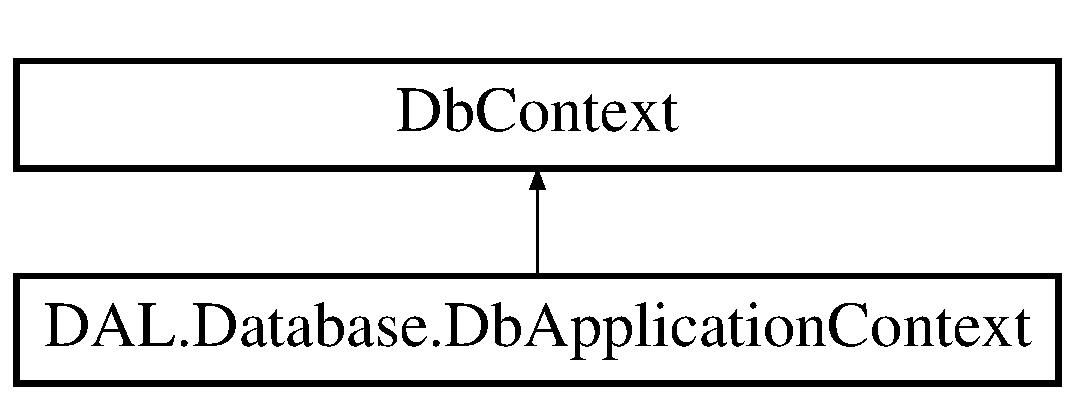
\includegraphics[height=2.000000cm]{class_d_a_l_1_1_database_1_1_db_application_context}
\end{center}
\end{figure}
\subsection*{Public Member Functions}
\begin{DoxyCompactItemize}
\item 
\hyperlink{class_d_a_l_1_1_database_1_1_db_application_context_ab5a2eb81194b1c06a325186fb3e5dbb1}{Db\+Application\+Context} ()
\begin{DoxyCompactList}\small\item\em Init the database \+: do not work with Sq\+Lite \end{DoxyCompactList}\end{DoxyCompactItemize}
\subsection*{Protected Member Functions}
\begin{DoxyCompactItemize}
\item 
override void \hyperlink{class_d_a_l_1_1_database_1_1_db_application_context_a19a77500b7e8ab9e3570a5abd81dc542}{On\+Model\+Creating} (Db\+Model\+Builder model\+Builder)
\begin{DoxyCompactList}\small\item\em Model the database \end{DoxyCompactList}\end{DoxyCompactItemize}
\subsection*{Properties}
\begin{DoxyCompactItemize}
\item 
\mbox{\Hypertarget{class_d_a_l_1_1_database_1_1_db_application_context_a5615f27c332c0393295c361b07c79d4f}\label{class_d_a_l_1_1_database_1_1_db_application_context_a5615f27c332c0393295c361b07c79d4f}} 
Db\+Set$<$ \hyperlink{class_d_t_o_1_1_entity_1_1_album}{Album} $>$ {\bfseries Album}\hspace{0.3cm}{\ttfamily  \mbox{[}get, set\mbox{]}}
\item 
\mbox{\Hypertarget{class_d_a_l_1_1_database_1_1_db_application_context_ad80a7e134c567d3df6b25b3753c9683a}\label{class_d_a_l_1_1_database_1_1_db_application_context_ad80a7e134c567d3df6b25b3753c9683a}} 
Db\+Set$<$ \hyperlink{class_d_t_o_1_1_entity_1_1_artist}{Artist} $>$ {\bfseries Artist}\hspace{0.3cm}{\ttfamily  \mbox{[}get, set\mbox{]}}
\item 
\mbox{\Hypertarget{class_d_a_l_1_1_database_1_1_db_application_context_af5ac4ddb073c13df72b8270643ffa6a1}\label{class_d_a_l_1_1_database_1_1_db_application_context_af5ac4ddb073c13df72b8270643ffa6a1}} 
Db\+Set$<$ \hyperlink{class_d_t_o_1_1_entity_1_1_context}{Context} $>$ {\bfseries Context}\hspace{0.3cm}{\ttfamily  \mbox{[}get, set\mbox{]}}
\item 
\mbox{\Hypertarget{class_d_a_l_1_1_database_1_1_db_application_context_afb4eed2364651f31d8b787d5a4c993ac}\label{class_d_a_l_1_1_database_1_1_db_application_context_afb4eed2364651f31d8b787d5a4c993ac}} 
Db\+Set$<$ \hyperlink{class_d_t_o_1_1_entity_1_1_genre}{Genre} $>$ {\bfseries Genre}\hspace{0.3cm}{\ttfamily  \mbox{[}get, set\mbox{]}}
\item 
\mbox{\Hypertarget{class_d_a_l_1_1_database_1_1_db_application_context_a7e71b8459ac910e2ebfa44cbbf6f5efc}\label{class_d_a_l_1_1_database_1_1_db_application_context_a7e71b8459ac910e2ebfa44cbbf6f5efc}} 
Db\+Set$<$ \hyperlink{class_d_t_o_1_1_entity_1_1_include_folder}{Include\+Folder} $>$ {\bfseries Include\+Folder}\hspace{0.3cm}{\ttfamily  \mbox{[}get, set\mbox{]}}
\item 
\mbox{\Hypertarget{class_d_a_l_1_1_database_1_1_db_application_context_a1041bf942933c80c1d4bb8a057bc2ca8}\label{class_d_a_l_1_1_database_1_1_db_application_context_a1041bf942933c80c1d4bb8a057bc2ca8}} 
Db\+Set$<$ \hyperlink{class_d_t_o_1_1_entity_1_1_playlist}{Playlist} $>$ {\bfseries Playlist}\hspace{0.3cm}{\ttfamily  \mbox{[}get, set\mbox{]}}
\item 
\mbox{\Hypertarget{class_d_a_l_1_1_database_1_1_db_application_context_a0d4bed5881215bd8fee58bf0dad84678}\label{class_d_a_l_1_1_database_1_1_db_application_context_a0d4bed5881215bd8fee58bf0dad84678}} 
Db\+Set$<$ \hyperlink{class_d_t_o_1_1_entity_1_1_radio}{Radio} $>$ {\bfseries Radio}\hspace{0.3cm}{\ttfamily  \mbox{[}get, set\mbox{]}}
\item 
\mbox{\Hypertarget{class_d_a_l_1_1_database_1_1_db_application_context_a3bce93761d2ab70e58a64da87675a80c}\label{class_d_a_l_1_1_database_1_1_db_application_context_a3bce93761d2ab70e58a64da87675a80c}} 
Db\+Set$<$ \hyperlink{class_d_t_o_1_1_entity_1_1_track}{Track} $>$ {\bfseries Track}\hspace{0.3cm}{\ttfamily  \mbox{[}get, set\mbox{]}}
\end{DoxyCompactItemize}


\subsection{Detailed Description}
Make the database connection 



\subsection{Constructor \& Destructor Documentation}
\mbox{\Hypertarget{class_d_a_l_1_1_database_1_1_db_application_context_ab5a2eb81194b1c06a325186fb3e5dbb1}\label{class_d_a_l_1_1_database_1_1_db_application_context_ab5a2eb81194b1c06a325186fb3e5dbb1}} 
\index{D\+A\+L\+::\+Database\+::\+Db\+Application\+Context@{D\+A\+L\+::\+Database\+::\+Db\+Application\+Context}!Db\+Application\+Context@{Db\+Application\+Context}}
\index{Db\+Application\+Context@{Db\+Application\+Context}!D\+A\+L\+::\+Database\+::\+Db\+Application\+Context@{D\+A\+L\+::\+Database\+::\+Db\+Application\+Context}}
\subsubsection{\texorpdfstring{Db\+Application\+Context()}{DbApplicationContext()}}
{\footnotesize\ttfamily D\+A\+L.\+Database.\+Db\+Application\+Context.\+Db\+Application\+Context (\begin{DoxyParamCaption}{ }\end{DoxyParamCaption})}



Init the database \+: do not work with Sq\+Lite 



\subsection{Member Function Documentation}
\mbox{\Hypertarget{class_d_a_l_1_1_database_1_1_db_application_context_a19a77500b7e8ab9e3570a5abd81dc542}\label{class_d_a_l_1_1_database_1_1_db_application_context_a19a77500b7e8ab9e3570a5abd81dc542}} 
\index{D\+A\+L\+::\+Database\+::\+Db\+Application\+Context@{D\+A\+L\+::\+Database\+::\+Db\+Application\+Context}!On\+Model\+Creating@{On\+Model\+Creating}}
\index{On\+Model\+Creating@{On\+Model\+Creating}!D\+A\+L\+::\+Database\+::\+Db\+Application\+Context@{D\+A\+L\+::\+Database\+::\+Db\+Application\+Context}}
\subsubsection{\texorpdfstring{On\+Model\+Creating()}{OnModelCreating()}}
{\footnotesize\ttfamily override void D\+A\+L.\+Database.\+Db\+Application\+Context.\+On\+Model\+Creating (\begin{DoxyParamCaption}\item[{Db\+Model\+Builder}]{model\+Builder }\end{DoxyParamCaption})\hspace{0.3cm}{\ttfamily [protected]}}



Model the database 


\begin{DoxyParams}{Parameters}
{\em model\+Builder} & \\
\hline
\end{DoxyParams}


The documentation for this class was generated from the following file\+:\begin{DoxyCompactItemize}
\item 
C\+:/\+W\+O\+R\+K\+S\+P\+A\+C\+E/\+T\+P\+I-\/end/\+Gestion\+Audio/\+D\+A\+L/\+Database/Db\+Context.\+cs\end{DoxyCompactItemize}

\hypertarget{class_presentation_1_1_view_1_1_list_1_1_favorite_list_view}{}\section{Presentation.\+View.\+List.\+Favorite\+List\+View Class Reference}
\label{class_presentation_1_1_view_1_1_list_1_1_favorite_list_view}\index{Presentation.\+View.\+List.\+Favorite\+List\+View@{Presentation.\+View.\+List.\+Favorite\+List\+View}}


\hyperlink{class_presentation_1_1_view_1_1_list_1_1_favorite_list_view}{Favorite\+List\+View}  


Inheritance diagram for Presentation.\+View.\+List.\+Favorite\+List\+View\+:\begin{figure}[H]
\begin{center}
\leavevmode
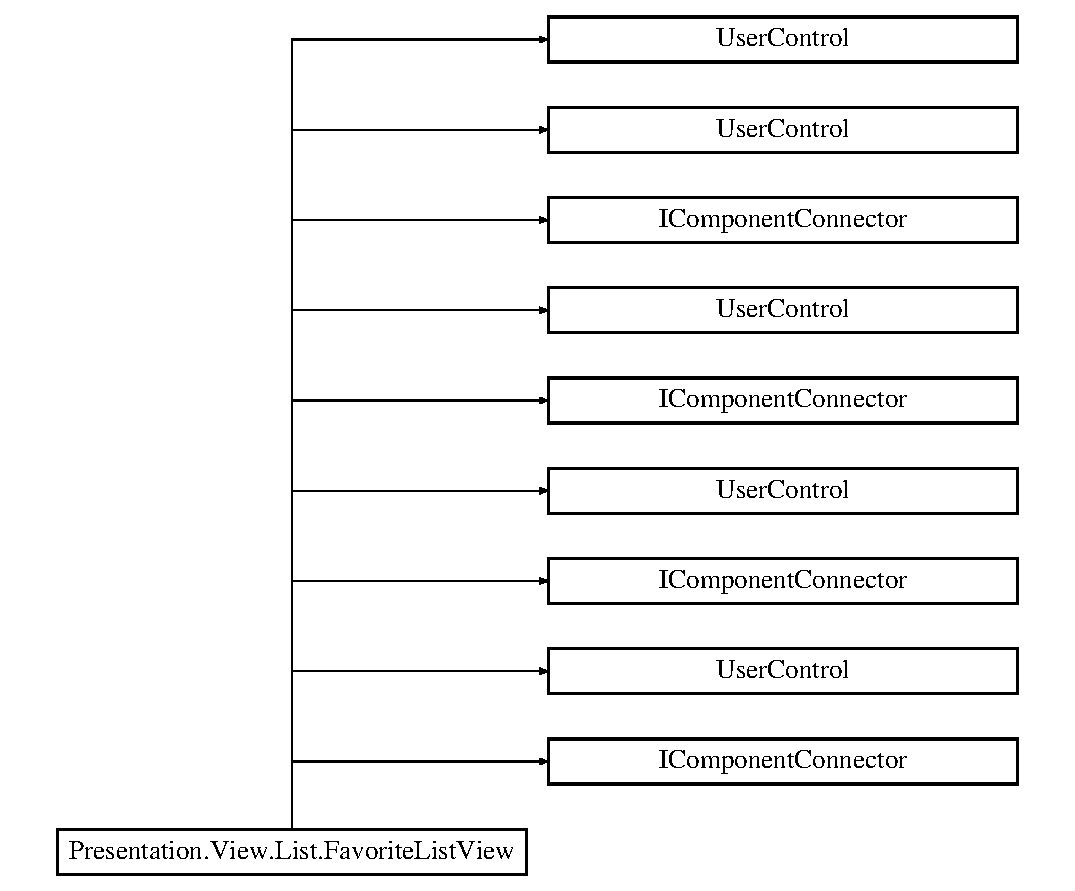
\includegraphics[height=10.000000cm]{class_presentation_1_1_view_1_1_list_1_1_favorite_list_view}
\end{center}
\end{figure}
\subsection*{Public Member Functions}
\begin{DoxyCompactItemize}
\item 
void \hyperlink{class_presentation_1_1_view_1_1_list_1_1_favorite_list_view_a63a1effe9695d3d0757c0b7144603ab5}{Initialize\+Component} ()
\begin{DoxyCompactList}\small\item\em Initialize\+Component \end{DoxyCompactList}\item 
void \hyperlink{class_presentation_1_1_view_1_1_list_1_1_favorite_list_view_a63a1effe9695d3d0757c0b7144603ab5}{Initialize\+Component} ()
\begin{DoxyCompactList}\small\item\em Initialize\+Component \end{DoxyCompactList}\item 
void \hyperlink{class_presentation_1_1_view_1_1_list_1_1_favorite_list_view_a63a1effe9695d3d0757c0b7144603ab5}{Initialize\+Component} ()
\begin{DoxyCompactList}\small\item\em Initialize\+Component \end{DoxyCompactList}\item 
void \hyperlink{class_presentation_1_1_view_1_1_list_1_1_favorite_list_view_a63a1effe9695d3d0757c0b7144603ab5}{Initialize\+Component} ()
\begin{DoxyCompactList}\small\item\em Initialize\+Component \end{DoxyCompactList}\end{DoxyCompactItemize}


\subsection{Detailed Description}
\hyperlink{class_presentation_1_1_view_1_1_list_1_1_favorite_list_view}{Favorite\+List\+View} 

Interaction logic for Music\+Home.\+xaml 

\subsection{Member Function Documentation}
\mbox{\Hypertarget{class_presentation_1_1_view_1_1_list_1_1_favorite_list_view_a63a1effe9695d3d0757c0b7144603ab5}\label{class_presentation_1_1_view_1_1_list_1_1_favorite_list_view_a63a1effe9695d3d0757c0b7144603ab5}} 
\index{Presentation\+::\+View\+::\+List\+::\+Favorite\+List\+View@{Presentation\+::\+View\+::\+List\+::\+Favorite\+List\+View}!Initialize\+Component@{Initialize\+Component}}
\index{Initialize\+Component@{Initialize\+Component}!Presentation\+::\+View\+::\+List\+::\+Favorite\+List\+View@{Presentation\+::\+View\+::\+List\+::\+Favorite\+List\+View}}
\subsubsection{\texorpdfstring{Initialize\+Component()}{InitializeComponent()}\hspace{0.1cm}{\footnotesize\ttfamily [1/4]}}
{\footnotesize\ttfamily void Presentation.\+View.\+List.\+Favorite\+List\+View.\+Initialize\+Component (\begin{DoxyParamCaption}{ }\end{DoxyParamCaption})}



Initialize\+Component 

\mbox{\Hypertarget{class_presentation_1_1_view_1_1_list_1_1_favorite_list_view_a63a1effe9695d3d0757c0b7144603ab5}\label{class_presentation_1_1_view_1_1_list_1_1_favorite_list_view_a63a1effe9695d3d0757c0b7144603ab5}} 
\index{Presentation\+::\+View\+::\+List\+::\+Favorite\+List\+View@{Presentation\+::\+View\+::\+List\+::\+Favorite\+List\+View}!Initialize\+Component@{Initialize\+Component}}
\index{Initialize\+Component@{Initialize\+Component}!Presentation\+::\+View\+::\+List\+::\+Favorite\+List\+View@{Presentation\+::\+View\+::\+List\+::\+Favorite\+List\+View}}
\subsubsection{\texorpdfstring{Initialize\+Component()}{InitializeComponent()}\hspace{0.1cm}{\footnotesize\ttfamily [2/4]}}
{\footnotesize\ttfamily void Presentation.\+View.\+List.\+Favorite\+List\+View.\+Initialize\+Component (\begin{DoxyParamCaption}{ }\end{DoxyParamCaption})}



Initialize\+Component 

\mbox{\Hypertarget{class_presentation_1_1_view_1_1_list_1_1_favorite_list_view_a63a1effe9695d3d0757c0b7144603ab5}\label{class_presentation_1_1_view_1_1_list_1_1_favorite_list_view_a63a1effe9695d3d0757c0b7144603ab5}} 
\index{Presentation\+::\+View\+::\+List\+::\+Favorite\+List\+View@{Presentation\+::\+View\+::\+List\+::\+Favorite\+List\+View}!Initialize\+Component@{Initialize\+Component}}
\index{Initialize\+Component@{Initialize\+Component}!Presentation\+::\+View\+::\+List\+::\+Favorite\+List\+View@{Presentation\+::\+View\+::\+List\+::\+Favorite\+List\+View}}
\subsubsection{\texorpdfstring{Initialize\+Component()}{InitializeComponent()}\hspace{0.1cm}{\footnotesize\ttfamily [3/4]}}
{\footnotesize\ttfamily void Presentation.\+View.\+List.\+Favorite\+List\+View.\+Initialize\+Component (\begin{DoxyParamCaption}{ }\end{DoxyParamCaption})}



Initialize\+Component 

\mbox{\Hypertarget{class_presentation_1_1_view_1_1_list_1_1_favorite_list_view_a63a1effe9695d3d0757c0b7144603ab5}\label{class_presentation_1_1_view_1_1_list_1_1_favorite_list_view_a63a1effe9695d3d0757c0b7144603ab5}} 
\index{Presentation\+::\+View\+::\+List\+::\+Favorite\+List\+View@{Presentation\+::\+View\+::\+List\+::\+Favorite\+List\+View}!Initialize\+Component@{Initialize\+Component}}
\index{Initialize\+Component@{Initialize\+Component}!Presentation\+::\+View\+::\+List\+::\+Favorite\+List\+View@{Presentation\+::\+View\+::\+List\+::\+Favorite\+List\+View}}
\subsubsection{\texorpdfstring{Initialize\+Component()}{InitializeComponent()}\hspace{0.1cm}{\footnotesize\ttfamily [4/4]}}
{\footnotesize\ttfamily void Presentation.\+View.\+List.\+Favorite\+List\+View.\+Initialize\+Component (\begin{DoxyParamCaption}{ }\end{DoxyParamCaption})}



Initialize\+Component 



The documentation for this class was generated from the following files\+:\begin{DoxyCompactItemize}
\item 
C\+:/\+W\+O\+R\+K\+S\+P\+A\+C\+E/\+T\+P\+I-\/end/\+Gestion\+Audio/\+Gestion\+Audio/obj/\+Debug/\+View/\+List/Favorite\+List\+View.\+g.\+cs\item 
C\+:/\+W\+O\+R\+K\+S\+P\+A\+C\+E/\+T\+P\+I-\/end/\+Gestion\+Audio/\+Gestion\+Audio/obj/\+Debug/\+View/\+List/Favorite\+List\+View.\+g.\+i.\+cs\item 
C\+:/\+W\+O\+R\+K\+S\+P\+A\+C\+E/\+T\+P\+I-\/end/\+Gestion\+Audio/\+Gestion\+Audio/\+View/\+List/Favorite\+List\+View.\+xaml.\+cs\end{DoxyCompactItemize}

\hypertarget{class_xaml_generated_namespace_1_1_generated_internal_type_helper}{}\section{Xaml\+Generated\+Namespace.\+Generated\+Internal\+Type\+Helper Class Reference}
\label{class_xaml_generated_namespace_1_1_generated_internal_type_helper}\index{Xaml\+Generated\+Namespace.\+Generated\+Internal\+Type\+Helper@{Xaml\+Generated\+Namespace.\+Generated\+Internal\+Type\+Helper}}


\hyperlink{class_xaml_generated_namespace_1_1_generated_internal_type_helper}{Generated\+Internal\+Type\+Helper}  


Inheritance diagram for Xaml\+Generated\+Namespace.\+Generated\+Internal\+Type\+Helper\+:\begin{figure}[H]
\begin{center}
\leavevmode
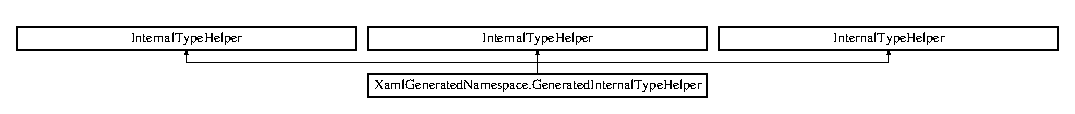
\includegraphics[height=1.085271cm]{class_xaml_generated_namespace_1_1_generated_internal_type_helper}
\end{center}
\end{figure}
\subsection*{Protected Member Functions}
\begin{DoxyCompactItemize}
\item 
override object \hyperlink{class_xaml_generated_namespace_1_1_generated_internal_type_helper_aefb7a98fceb9c287cef4756942f441d1}{Create\+Instance} (System.\+Type type, System.\+Globalization.\+Culture\+Info culture)
\begin{DoxyCompactList}\small\item\em Create\+Instance \end{DoxyCompactList}\item 
override object \hyperlink{class_xaml_generated_namespace_1_1_generated_internal_type_helper_afdc9fe15b56607d02082908d934480c6}{Get\+Property\+Value} (System.\+Reflection.\+Property\+Info property\+Info, object target, System.\+Globalization.\+Culture\+Info culture)
\begin{DoxyCompactList}\small\item\em Get\+Property\+Value \end{DoxyCompactList}\item 
override void \hyperlink{class_xaml_generated_namespace_1_1_generated_internal_type_helper_ade0f04c0f7b18dd5b170e071d5534d38}{Set\+Property\+Value} (System.\+Reflection.\+Property\+Info property\+Info, object target, object value, System.\+Globalization.\+Culture\+Info culture)
\begin{DoxyCompactList}\small\item\em Set\+Property\+Value \end{DoxyCompactList}\item 
override System.\+Delegate \hyperlink{class_xaml_generated_namespace_1_1_generated_internal_type_helper_a8ec4c37e82d9f4e867e9655f4eac3a78}{Create\+Delegate} (System.\+Type delegate\+Type, object target, string handler)
\begin{DoxyCompactList}\small\item\em Create\+Delegate \end{DoxyCompactList}\item 
override void \hyperlink{class_xaml_generated_namespace_1_1_generated_internal_type_helper_a73471f4a6d1ca4c4fceec9ad8610f0c8}{Add\+Event\+Handler} (System.\+Reflection.\+Event\+Info event\+Info, object target, System.\+Delegate handler)
\begin{DoxyCompactList}\small\item\em Add\+Event\+Handler \end{DoxyCompactList}\item 
override object \hyperlink{class_xaml_generated_namespace_1_1_generated_internal_type_helper_aefb7a98fceb9c287cef4756942f441d1}{Create\+Instance} (System.\+Type type, System.\+Globalization.\+Culture\+Info culture)
\begin{DoxyCompactList}\small\item\em Create\+Instance \end{DoxyCompactList}\item 
override object \hyperlink{class_xaml_generated_namespace_1_1_generated_internal_type_helper_afdc9fe15b56607d02082908d934480c6}{Get\+Property\+Value} (System.\+Reflection.\+Property\+Info property\+Info, object target, System.\+Globalization.\+Culture\+Info culture)
\begin{DoxyCompactList}\small\item\em Get\+Property\+Value \end{DoxyCompactList}\item 
override void \hyperlink{class_xaml_generated_namespace_1_1_generated_internal_type_helper_ade0f04c0f7b18dd5b170e071d5534d38}{Set\+Property\+Value} (System.\+Reflection.\+Property\+Info property\+Info, object target, object value, System.\+Globalization.\+Culture\+Info culture)
\begin{DoxyCompactList}\small\item\em Set\+Property\+Value \end{DoxyCompactList}\item 
override System.\+Delegate \hyperlink{class_xaml_generated_namespace_1_1_generated_internal_type_helper_a8ec4c37e82d9f4e867e9655f4eac3a78}{Create\+Delegate} (System.\+Type delegate\+Type, object target, string handler)
\begin{DoxyCompactList}\small\item\em Create\+Delegate \end{DoxyCompactList}\item 
override void \hyperlink{class_xaml_generated_namespace_1_1_generated_internal_type_helper_a73471f4a6d1ca4c4fceec9ad8610f0c8}{Add\+Event\+Handler} (System.\+Reflection.\+Event\+Info event\+Info, object target, System.\+Delegate handler)
\begin{DoxyCompactList}\small\item\em Add\+Event\+Handler \end{DoxyCompactList}\item 
override object \hyperlink{class_xaml_generated_namespace_1_1_generated_internal_type_helper_aefb7a98fceb9c287cef4756942f441d1}{Create\+Instance} (System.\+Type type, System.\+Globalization.\+Culture\+Info culture)
\begin{DoxyCompactList}\small\item\em Create\+Instance \end{DoxyCompactList}\item 
override object \hyperlink{class_xaml_generated_namespace_1_1_generated_internal_type_helper_afdc9fe15b56607d02082908d934480c6}{Get\+Property\+Value} (System.\+Reflection.\+Property\+Info property\+Info, object target, System.\+Globalization.\+Culture\+Info culture)
\begin{DoxyCompactList}\small\item\em Get\+Property\+Value \end{DoxyCompactList}\item 
override void \hyperlink{class_xaml_generated_namespace_1_1_generated_internal_type_helper_ade0f04c0f7b18dd5b170e071d5534d38}{Set\+Property\+Value} (System.\+Reflection.\+Property\+Info property\+Info, object target, object value, System.\+Globalization.\+Culture\+Info culture)
\begin{DoxyCompactList}\small\item\em Set\+Property\+Value \end{DoxyCompactList}\item 
override System.\+Delegate \hyperlink{class_xaml_generated_namespace_1_1_generated_internal_type_helper_a8ec4c37e82d9f4e867e9655f4eac3a78}{Create\+Delegate} (System.\+Type delegate\+Type, object target, string handler)
\begin{DoxyCompactList}\small\item\em Create\+Delegate \end{DoxyCompactList}\item 
override void \hyperlink{class_xaml_generated_namespace_1_1_generated_internal_type_helper_a73471f4a6d1ca4c4fceec9ad8610f0c8}{Add\+Event\+Handler} (System.\+Reflection.\+Event\+Info event\+Info, object target, System.\+Delegate handler)
\begin{DoxyCompactList}\small\item\em Add\+Event\+Handler \end{DoxyCompactList}\end{DoxyCompactItemize}


\subsection{Detailed Description}
\hyperlink{class_xaml_generated_namespace_1_1_generated_internal_type_helper}{Generated\+Internal\+Type\+Helper} 



\subsection{Member Function Documentation}
\mbox{\Hypertarget{class_xaml_generated_namespace_1_1_generated_internal_type_helper_a73471f4a6d1ca4c4fceec9ad8610f0c8}\label{class_xaml_generated_namespace_1_1_generated_internal_type_helper_a73471f4a6d1ca4c4fceec9ad8610f0c8}} 
\index{Xaml\+Generated\+Namespace\+::\+Generated\+Internal\+Type\+Helper@{Xaml\+Generated\+Namespace\+::\+Generated\+Internal\+Type\+Helper}!Add\+Event\+Handler@{Add\+Event\+Handler}}
\index{Add\+Event\+Handler@{Add\+Event\+Handler}!Xaml\+Generated\+Namespace\+::\+Generated\+Internal\+Type\+Helper@{Xaml\+Generated\+Namespace\+::\+Generated\+Internal\+Type\+Helper}}
\subsubsection{\texorpdfstring{Add\+Event\+Handler()}{AddEventHandler()}\hspace{0.1cm}{\footnotesize\ttfamily [1/3]}}
{\footnotesize\ttfamily override void Xaml\+Generated\+Namespace.\+Generated\+Internal\+Type\+Helper.\+Add\+Event\+Handler (\begin{DoxyParamCaption}\item[{System.\+Reflection.\+Event\+Info}]{event\+Info,  }\item[{object}]{target,  }\item[{System.\+Delegate}]{handler }\end{DoxyParamCaption})\hspace{0.3cm}{\ttfamily [protected]}}



Add\+Event\+Handler 

\mbox{\Hypertarget{class_xaml_generated_namespace_1_1_generated_internal_type_helper_a73471f4a6d1ca4c4fceec9ad8610f0c8}\label{class_xaml_generated_namespace_1_1_generated_internal_type_helper_a73471f4a6d1ca4c4fceec9ad8610f0c8}} 
\index{Xaml\+Generated\+Namespace\+::\+Generated\+Internal\+Type\+Helper@{Xaml\+Generated\+Namespace\+::\+Generated\+Internal\+Type\+Helper}!Add\+Event\+Handler@{Add\+Event\+Handler}}
\index{Add\+Event\+Handler@{Add\+Event\+Handler}!Xaml\+Generated\+Namespace\+::\+Generated\+Internal\+Type\+Helper@{Xaml\+Generated\+Namespace\+::\+Generated\+Internal\+Type\+Helper}}
\subsubsection{\texorpdfstring{Add\+Event\+Handler()}{AddEventHandler()}\hspace{0.1cm}{\footnotesize\ttfamily [2/3]}}
{\footnotesize\ttfamily override void Xaml\+Generated\+Namespace.\+Generated\+Internal\+Type\+Helper.\+Add\+Event\+Handler (\begin{DoxyParamCaption}\item[{System.\+Reflection.\+Event\+Info}]{event\+Info,  }\item[{object}]{target,  }\item[{System.\+Delegate}]{handler }\end{DoxyParamCaption})\hspace{0.3cm}{\ttfamily [protected]}}



Add\+Event\+Handler 

\mbox{\Hypertarget{class_xaml_generated_namespace_1_1_generated_internal_type_helper_a73471f4a6d1ca4c4fceec9ad8610f0c8}\label{class_xaml_generated_namespace_1_1_generated_internal_type_helper_a73471f4a6d1ca4c4fceec9ad8610f0c8}} 
\index{Xaml\+Generated\+Namespace\+::\+Generated\+Internal\+Type\+Helper@{Xaml\+Generated\+Namespace\+::\+Generated\+Internal\+Type\+Helper}!Add\+Event\+Handler@{Add\+Event\+Handler}}
\index{Add\+Event\+Handler@{Add\+Event\+Handler}!Xaml\+Generated\+Namespace\+::\+Generated\+Internal\+Type\+Helper@{Xaml\+Generated\+Namespace\+::\+Generated\+Internal\+Type\+Helper}}
\subsubsection{\texorpdfstring{Add\+Event\+Handler()}{AddEventHandler()}\hspace{0.1cm}{\footnotesize\ttfamily [3/3]}}
{\footnotesize\ttfamily override void Xaml\+Generated\+Namespace.\+Generated\+Internal\+Type\+Helper.\+Add\+Event\+Handler (\begin{DoxyParamCaption}\item[{System.\+Reflection.\+Event\+Info}]{event\+Info,  }\item[{object}]{target,  }\item[{System.\+Delegate}]{handler }\end{DoxyParamCaption})\hspace{0.3cm}{\ttfamily [protected]}}



Add\+Event\+Handler 

\mbox{\Hypertarget{class_xaml_generated_namespace_1_1_generated_internal_type_helper_a8ec4c37e82d9f4e867e9655f4eac3a78}\label{class_xaml_generated_namespace_1_1_generated_internal_type_helper_a8ec4c37e82d9f4e867e9655f4eac3a78}} 
\index{Xaml\+Generated\+Namespace\+::\+Generated\+Internal\+Type\+Helper@{Xaml\+Generated\+Namespace\+::\+Generated\+Internal\+Type\+Helper}!Create\+Delegate@{Create\+Delegate}}
\index{Create\+Delegate@{Create\+Delegate}!Xaml\+Generated\+Namespace\+::\+Generated\+Internal\+Type\+Helper@{Xaml\+Generated\+Namespace\+::\+Generated\+Internal\+Type\+Helper}}
\subsubsection{\texorpdfstring{Create\+Delegate()}{CreateDelegate()}\hspace{0.1cm}{\footnotesize\ttfamily [1/3]}}
{\footnotesize\ttfamily override System.\+Delegate Xaml\+Generated\+Namespace.\+Generated\+Internal\+Type\+Helper.\+Create\+Delegate (\begin{DoxyParamCaption}\item[{System.\+Type}]{delegate\+Type,  }\item[{object}]{target,  }\item[{string}]{handler }\end{DoxyParamCaption})\hspace{0.3cm}{\ttfamily [protected]}}



Create\+Delegate 

\mbox{\Hypertarget{class_xaml_generated_namespace_1_1_generated_internal_type_helper_a8ec4c37e82d9f4e867e9655f4eac3a78}\label{class_xaml_generated_namespace_1_1_generated_internal_type_helper_a8ec4c37e82d9f4e867e9655f4eac3a78}} 
\index{Xaml\+Generated\+Namespace\+::\+Generated\+Internal\+Type\+Helper@{Xaml\+Generated\+Namespace\+::\+Generated\+Internal\+Type\+Helper}!Create\+Delegate@{Create\+Delegate}}
\index{Create\+Delegate@{Create\+Delegate}!Xaml\+Generated\+Namespace\+::\+Generated\+Internal\+Type\+Helper@{Xaml\+Generated\+Namespace\+::\+Generated\+Internal\+Type\+Helper}}
\subsubsection{\texorpdfstring{Create\+Delegate()}{CreateDelegate()}\hspace{0.1cm}{\footnotesize\ttfamily [2/3]}}
{\footnotesize\ttfamily override System.\+Delegate Xaml\+Generated\+Namespace.\+Generated\+Internal\+Type\+Helper.\+Create\+Delegate (\begin{DoxyParamCaption}\item[{System.\+Type}]{delegate\+Type,  }\item[{object}]{target,  }\item[{string}]{handler }\end{DoxyParamCaption})\hspace{0.3cm}{\ttfamily [protected]}}



Create\+Delegate 

\mbox{\Hypertarget{class_xaml_generated_namespace_1_1_generated_internal_type_helper_a8ec4c37e82d9f4e867e9655f4eac3a78}\label{class_xaml_generated_namespace_1_1_generated_internal_type_helper_a8ec4c37e82d9f4e867e9655f4eac3a78}} 
\index{Xaml\+Generated\+Namespace\+::\+Generated\+Internal\+Type\+Helper@{Xaml\+Generated\+Namespace\+::\+Generated\+Internal\+Type\+Helper}!Create\+Delegate@{Create\+Delegate}}
\index{Create\+Delegate@{Create\+Delegate}!Xaml\+Generated\+Namespace\+::\+Generated\+Internal\+Type\+Helper@{Xaml\+Generated\+Namespace\+::\+Generated\+Internal\+Type\+Helper}}
\subsubsection{\texorpdfstring{Create\+Delegate()}{CreateDelegate()}\hspace{0.1cm}{\footnotesize\ttfamily [3/3]}}
{\footnotesize\ttfamily override System.\+Delegate Xaml\+Generated\+Namespace.\+Generated\+Internal\+Type\+Helper.\+Create\+Delegate (\begin{DoxyParamCaption}\item[{System.\+Type}]{delegate\+Type,  }\item[{object}]{target,  }\item[{string}]{handler }\end{DoxyParamCaption})\hspace{0.3cm}{\ttfamily [protected]}}



Create\+Delegate 

\mbox{\Hypertarget{class_xaml_generated_namespace_1_1_generated_internal_type_helper_aefb7a98fceb9c287cef4756942f441d1}\label{class_xaml_generated_namespace_1_1_generated_internal_type_helper_aefb7a98fceb9c287cef4756942f441d1}} 
\index{Xaml\+Generated\+Namespace\+::\+Generated\+Internal\+Type\+Helper@{Xaml\+Generated\+Namespace\+::\+Generated\+Internal\+Type\+Helper}!Create\+Instance@{Create\+Instance}}
\index{Create\+Instance@{Create\+Instance}!Xaml\+Generated\+Namespace\+::\+Generated\+Internal\+Type\+Helper@{Xaml\+Generated\+Namespace\+::\+Generated\+Internal\+Type\+Helper}}
\subsubsection{\texorpdfstring{Create\+Instance()}{CreateInstance()}\hspace{0.1cm}{\footnotesize\ttfamily [1/3]}}
{\footnotesize\ttfamily override object Xaml\+Generated\+Namespace.\+Generated\+Internal\+Type\+Helper.\+Create\+Instance (\begin{DoxyParamCaption}\item[{System.\+Type}]{type,  }\item[{System.\+Globalization.\+Culture\+Info}]{culture }\end{DoxyParamCaption})\hspace{0.3cm}{\ttfamily [protected]}}



Create\+Instance 

\mbox{\Hypertarget{class_xaml_generated_namespace_1_1_generated_internal_type_helper_aefb7a98fceb9c287cef4756942f441d1}\label{class_xaml_generated_namespace_1_1_generated_internal_type_helper_aefb7a98fceb9c287cef4756942f441d1}} 
\index{Xaml\+Generated\+Namespace\+::\+Generated\+Internal\+Type\+Helper@{Xaml\+Generated\+Namespace\+::\+Generated\+Internal\+Type\+Helper}!Create\+Instance@{Create\+Instance}}
\index{Create\+Instance@{Create\+Instance}!Xaml\+Generated\+Namespace\+::\+Generated\+Internal\+Type\+Helper@{Xaml\+Generated\+Namespace\+::\+Generated\+Internal\+Type\+Helper}}
\subsubsection{\texorpdfstring{Create\+Instance()}{CreateInstance()}\hspace{0.1cm}{\footnotesize\ttfamily [2/3]}}
{\footnotesize\ttfamily override object Xaml\+Generated\+Namespace.\+Generated\+Internal\+Type\+Helper.\+Create\+Instance (\begin{DoxyParamCaption}\item[{System.\+Type}]{type,  }\item[{System.\+Globalization.\+Culture\+Info}]{culture }\end{DoxyParamCaption})\hspace{0.3cm}{\ttfamily [protected]}}



Create\+Instance 

\mbox{\Hypertarget{class_xaml_generated_namespace_1_1_generated_internal_type_helper_aefb7a98fceb9c287cef4756942f441d1}\label{class_xaml_generated_namespace_1_1_generated_internal_type_helper_aefb7a98fceb9c287cef4756942f441d1}} 
\index{Xaml\+Generated\+Namespace\+::\+Generated\+Internal\+Type\+Helper@{Xaml\+Generated\+Namespace\+::\+Generated\+Internal\+Type\+Helper}!Create\+Instance@{Create\+Instance}}
\index{Create\+Instance@{Create\+Instance}!Xaml\+Generated\+Namespace\+::\+Generated\+Internal\+Type\+Helper@{Xaml\+Generated\+Namespace\+::\+Generated\+Internal\+Type\+Helper}}
\subsubsection{\texorpdfstring{Create\+Instance()}{CreateInstance()}\hspace{0.1cm}{\footnotesize\ttfamily [3/3]}}
{\footnotesize\ttfamily override object Xaml\+Generated\+Namespace.\+Generated\+Internal\+Type\+Helper.\+Create\+Instance (\begin{DoxyParamCaption}\item[{System.\+Type}]{type,  }\item[{System.\+Globalization.\+Culture\+Info}]{culture }\end{DoxyParamCaption})\hspace{0.3cm}{\ttfamily [protected]}}



Create\+Instance 

\mbox{\Hypertarget{class_xaml_generated_namespace_1_1_generated_internal_type_helper_afdc9fe15b56607d02082908d934480c6}\label{class_xaml_generated_namespace_1_1_generated_internal_type_helper_afdc9fe15b56607d02082908d934480c6}} 
\index{Xaml\+Generated\+Namespace\+::\+Generated\+Internal\+Type\+Helper@{Xaml\+Generated\+Namespace\+::\+Generated\+Internal\+Type\+Helper}!Get\+Property\+Value@{Get\+Property\+Value}}
\index{Get\+Property\+Value@{Get\+Property\+Value}!Xaml\+Generated\+Namespace\+::\+Generated\+Internal\+Type\+Helper@{Xaml\+Generated\+Namespace\+::\+Generated\+Internal\+Type\+Helper}}
\subsubsection{\texorpdfstring{Get\+Property\+Value()}{GetPropertyValue()}\hspace{0.1cm}{\footnotesize\ttfamily [1/3]}}
{\footnotesize\ttfamily override object Xaml\+Generated\+Namespace.\+Generated\+Internal\+Type\+Helper.\+Get\+Property\+Value (\begin{DoxyParamCaption}\item[{System.\+Reflection.\+Property\+Info}]{property\+Info,  }\item[{object}]{target,  }\item[{System.\+Globalization.\+Culture\+Info}]{culture }\end{DoxyParamCaption})\hspace{0.3cm}{\ttfamily [protected]}}



Get\+Property\+Value 

\mbox{\Hypertarget{class_xaml_generated_namespace_1_1_generated_internal_type_helper_afdc9fe15b56607d02082908d934480c6}\label{class_xaml_generated_namespace_1_1_generated_internal_type_helper_afdc9fe15b56607d02082908d934480c6}} 
\index{Xaml\+Generated\+Namespace\+::\+Generated\+Internal\+Type\+Helper@{Xaml\+Generated\+Namespace\+::\+Generated\+Internal\+Type\+Helper}!Get\+Property\+Value@{Get\+Property\+Value}}
\index{Get\+Property\+Value@{Get\+Property\+Value}!Xaml\+Generated\+Namespace\+::\+Generated\+Internal\+Type\+Helper@{Xaml\+Generated\+Namespace\+::\+Generated\+Internal\+Type\+Helper}}
\subsubsection{\texorpdfstring{Get\+Property\+Value()}{GetPropertyValue()}\hspace{0.1cm}{\footnotesize\ttfamily [2/3]}}
{\footnotesize\ttfamily override object Xaml\+Generated\+Namespace.\+Generated\+Internal\+Type\+Helper.\+Get\+Property\+Value (\begin{DoxyParamCaption}\item[{System.\+Reflection.\+Property\+Info}]{property\+Info,  }\item[{object}]{target,  }\item[{System.\+Globalization.\+Culture\+Info}]{culture }\end{DoxyParamCaption})\hspace{0.3cm}{\ttfamily [protected]}}



Get\+Property\+Value 

\mbox{\Hypertarget{class_xaml_generated_namespace_1_1_generated_internal_type_helper_afdc9fe15b56607d02082908d934480c6}\label{class_xaml_generated_namespace_1_1_generated_internal_type_helper_afdc9fe15b56607d02082908d934480c6}} 
\index{Xaml\+Generated\+Namespace\+::\+Generated\+Internal\+Type\+Helper@{Xaml\+Generated\+Namespace\+::\+Generated\+Internal\+Type\+Helper}!Get\+Property\+Value@{Get\+Property\+Value}}
\index{Get\+Property\+Value@{Get\+Property\+Value}!Xaml\+Generated\+Namespace\+::\+Generated\+Internal\+Type\+Helper@{Xaml\+Generated\+Namespace\+::\+Generated\+Internal\+Type\+Helper}}
\subsubsection{\texorpdfstring{Get\+Property\+Value()}{GetPropertyValue()}\hspace{0.1cm}{\footnotesize\ttfamily [3/3]}}
{\footnotesize\ttfamily override object Xaml\+Generated\+Namespace.\+Generated\+Internal\+Type\+Helper.\+Get\+Property\+Value (\begin{DoxyParamCaption}\item[{System.\+Reflection.\+Property\+Info}]{property\+Info,  }\item[{object}]{target,  }\item[{System.\+Globalization.\+Culture\+Info}]{culture }\end{DoxyParamCaption})\hspace{0.3cm}{\ttfamily [protected]}}



Get\+Property\+Value 

\mbox{\Hypertarget{class_xaml_generated_namespace_1_1_generated_internal_type_helper_ade0f04c0f7b18dd5b170e071d5534d38}\label{class_xaml_generated_namespace_1_1_generated_internal_type_helper_ade0f04c0f7b18dd5b170e071d5534d38}} 
\index{Xaml\+Generated\+Namespace\+::\+Generated\+Internal\+Type\+Helper@{Xaml\+Generated\+Namespace\+::\+Generated\+Internal\+Type\+Helper}!Set\+Property\+Value@{Set\+Property\+Value}}
\index{Set\+Property\+Value@{Set\+Property\+Value}!Xaml\+Generated\+Namespace\+::\+Generated\+Internal\+Type\+Helper@{Xaml\+Generated\+Namespace\+::\+Generated\+Internal\+Type\+Helper}}
\subsubsection{\texorpdfstring{Set\+Property\+Value()}{SetPropertyValue()}\hspace{0.1cm}{\footnotesize\ttfamily [1/3]}}
{\footnotesize\ttfamily override void Xaml\+Generated\+Namespace.\+Generated\+Internal\+Type\+Helper.\+Set\+Property\+Value (\begin{DoxyParamCaption}\item[{System.\+Reflection.\+Property\+Info}]{property\+Info,  }\item[{object}]{target,  }\item[{object}]{value,  }\item[{System.\+Globalization.\+Culture\+Info}]{culture }\end{DoxyParamCaption})\hspace{0.3cm}{\ttfamily [protected]}}



Set\+Property\+Value 

\mbox{\Hypertarget{class_xaml_generated_namespace_1_1_generated_internal_type_helper_ade0f04c0f7b18dd5b170e071d5534d38}\label{class_xaml_generated_namespace_1_1_generated_internal_type_helper_ade0f04c0f7b18dd5b170e071d5534d38}} 
\index{Xaml\+Generated\+Namespace\+::\+Generated\+Internal\+Type\+Helper@{Xaml\+Generated\+Namespace\+::\+Generated\+Internal\+Type\+Helper}!Set\+Property\+Value@{Set\+Property\+Value}}
\index{Set\+Property\+Value@{Set\+Property\+Value}!Xaml\+Generated\+Namespace\+::\+Generated\+Internal\+Type\+Helper@{Xaml\+Generated\+Namespace\+::\+Generated\+Internal\+Type\+Helper}}
\subsubsection{\texorpdfstring{Set\+Property\+Value()}{SetPropertyValue()}\hspace{0.1cm}{\footnotesize\ttfamily [2/3]}}
{\footnotesize\ttfamily override void Xaml\+Generated\+Namespace.\+Generated\+Internal\+Type\+Helper.\+Set\+Property\+Value (\begin{DoxyParamCaption}\item[{System.\+Reflection.\+Property\+Info}]{property\+Info,  }\item[{object}]{target,  }\item[{object}]{value,  }\item[{System.\+Globalization.\+Culture\+Info}]{culture }\end{DoxyParamCaption})\hspace{0.3cm}{\ttfamily [protected]}}



Set\+Property\+Value 

\mbox{\Hypertarget{class_xaml_generated_namespace_1_1_generated_internal_type_helper_ade0f04c0f7b18dd5b170e071d5534d38}\label{class_xaml_generated_namespace_1_1_generated_internal_type_helper_ade0f04c0f7b18dd5b170e071d5534d38}} 
\index{Xaml\+Generated\+Namespace\+::\+Generated\+Internal\+Type\+Helper@{Xaml\+Generated\+Namespace\+::\+Generated\+Internal\+Type\+Helper}!Set\+Property\+Value@{Set\+Property\+Value}}
\index{Set\+Property\+Value@{Set\+Property\+Value}!Xaml\+Generated\+Namespace\+::\+Generated\+Internal\+Type\+Helper@{Xaml\+Generated\+Namespace\+::\+Generated\+Internal\+Type\+Helper}}
\subsubsection{\texorpdfstring{Set\+Property\+Value()}{SetPropertyValue()}\hspace{0.1cm}{\footnotesize\ttfamily [3/3]}}
{\footnotesize\ttfamily override void Xaml\+Generated\+Namespace.\+Generated\+Internal\+Type\+Helper.\+Set\+Property\+Value (\begin{DoxyParamCaption}\item[{System.\+Reflection.\+Property\+Info}]{property\+Info,  }\item[{object}]{target,  }\item[{object}]{value,  }\item[{System.\+Globalization.\+Culture\+Info}]{culture }\end{DoxyParamCaption})\hspace{0.3cm}{\ttfamily [protected]}}



Set\+Property\+Value 



The documentation for this class was generated from the following files\+:\begin{DoxyCompactItemize}
\item 
C\+:/\+W\+O\+R\+K\+S\+P\+A\+C\+E/\+T\+P\+I-\/end/\+Gestion\+Audio/\+Gestion\+Audio/obj/\+Debug/Generated\+Internal\+Type\+Helper.\+g.\+cs\item 
C\+:/\+W\+O\+R\+K\+S\+P\+A\+C\+E/\+T\+P\+I-\/end/\+Gestion\+Audio/\+Gestion\+Audio/obj/\+Debug/Generated\+Internal\+Type\+Helper.\+g.\+i.\+cs\end{DoxyCompactItemize}

\hypertarget{class_d_t_o_1_1_entity_1_1_genre}{}\section{D\+T\+O.\+Entity.\+Genre Class Reference}
\label{class_d_t_o_1_1_entity_1_1_genre}\index{D\+T\+O.\+Entity.\+Genre@{D\+T\+O.\+Entity.\+Genre}}


The database \hyperlink{class_d_t_o_1_1_entity_1_1_genre}{Genre} entity  


Inheritance diagram for D\+T\+O.\+Entity.\+Genre\+:\begin{figure}[H]
\begin{center}
\leavevmode
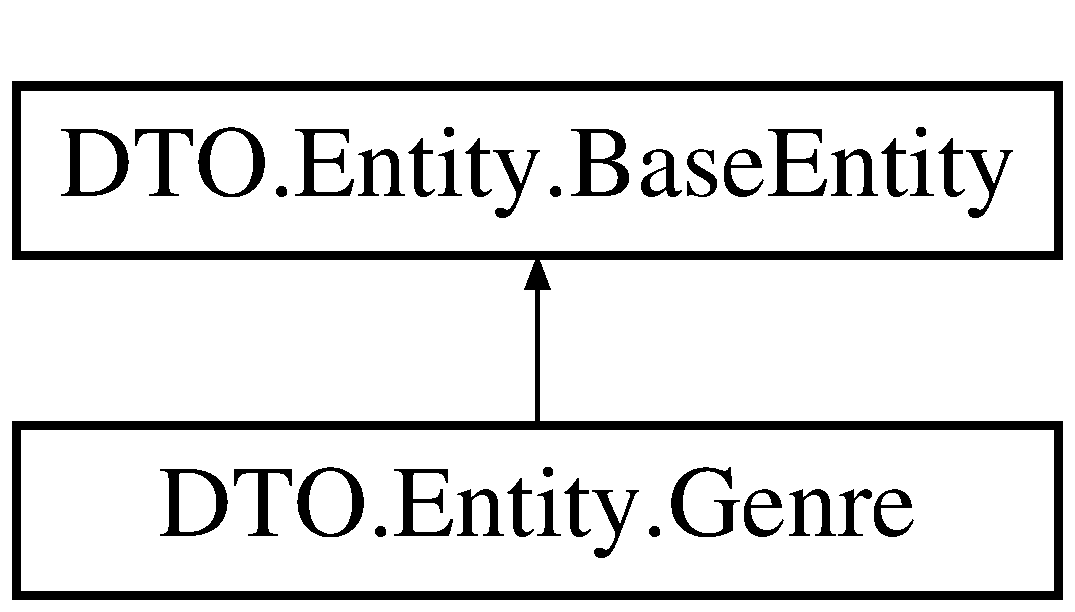
\includegraphics[height=2.000000cm]{class_d_t_o_1_1_entity_1_1_genre}
\end{center}
\end{figure}
\subsection*{Properties}
\begin{DoxyCompactItemize}
\item 
\mbox{\Hypertarget{class_d_t_o_1_1_entity_1_1_genre_a11a7f942944499fd58d55d3e9efe2407}\label{class_d_t_o_1_1_entity_1_1_genre_a11a7f942944499fd58d55d3e9efe2407}} 
int {\bfseries Listened\+Times}\hspace{0.3cm}{\ttfamily  \mbox{[}get, set\mbox{]}}
\item 
\mbox{\Hypertarget{class_d_t_o_1_1_entity_1_1_genre_a62c9a9e23570e2eeb8c7df13085cd9ff}\label{class_d_t_o_1_1_entity_1_1_genre_a62c9a9e23570e2eeb8c7df13085cd9ff}} 
string {\bfseries Name}\hspace{0.3cm}{\ttfamily  \mbox{[}get, set\mbox{]}}
\item 
\mbox{\Hypertarget{class_d_t_o_1_1_entity_1_1_genre_a5be3ef9a7c0a7c002041a91262055690}\label{class_d_t_o_1_1_entity_1_1_genre_a5be3ef9a7c0a7c002041a91262055690}} 
virtual I\+Collection$<$ \hyperlink{class_d_t_o_1_1_entity_1_1_track}{Track} $>$ {\bfseries Tracks}\hspace{0.3cm}{\ttfamily  \mbox{[}get, set\mbox{]}}
\end{DoxyCompactItemize}


\subsection{Detailed Description}
The database \hyperlink{class_d_t_o_1_1_entity_1_1_genre}{Genre} entity 



The documentation for this class was generated from the following file\+:\begin{DoxyCompactItemize}
\item 
C\+:/\+W\+O\+R\+K\+S\+P\+A\+C\+E/\+T\+P\+I-\/end/\+Gestion\+Audio/\+D\+T\+O/\+Entity/Genre.\+cs\end{DoxyCompactItemize}

\hypertarget{class_presentation_1_1_view_1_1_list_1_1_genre_list_view}{}\section{Presentation.\+View.\+List.\+Genre\+List\+View Class Reference}
\label{class_presentation_1_1_view_1_1_list_1_1_genre_list_view}\index{Presentation.\+View.\+List.\+Genre\+List\+View@{Presentation.\+View.\+List.\+Genre\+List\+View}}


\hyperlink{class_presentation_1_1_view_1_1_list_1_1_genre_list_view}{Genre\+List\+View}  


Inheritance diagram for Presentation.\+View.\+List.\+Genre\+List\+View\+:\begin{figure}[H]
\begin{center}
\leavevmode
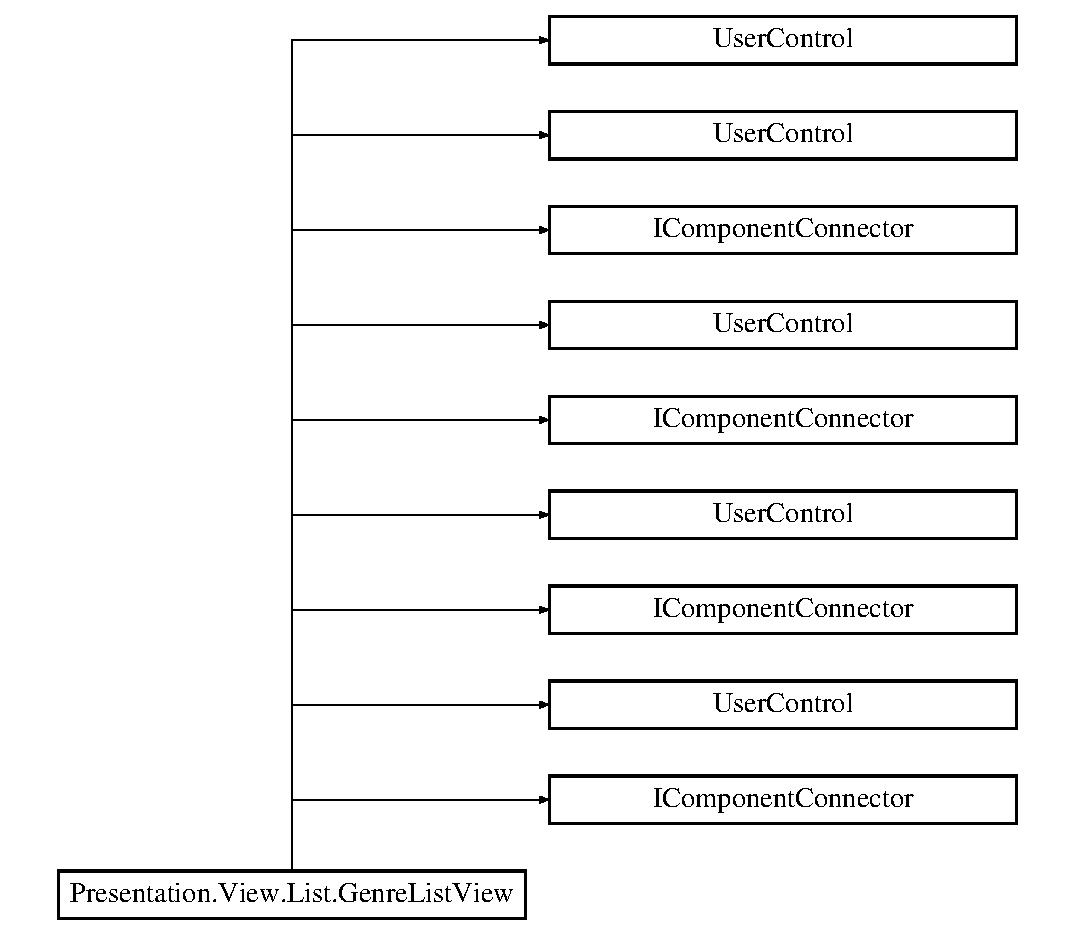
\includegraphics[height=10.000000cm]{class_presentation_1_1_view_1_1_list_1_1_genre_list_view}
\end{center}
\end{figure}
\subsection*{Public Member Functions}
\begin{DoxyCompactItemize}
\item 
void \hyperlink{class_presentation_1_1_view_1_1_list_1_1_genre_list_view_a5f6099fc62c1c6be505c094bacca79ca}{Initialize\+Component} ()
\begin{DoxyCompactList}\small\item\em Initialize\+Component \end{DoxyCompactList}\item 
void \hyperlink{class_presentation_1_1_view_1_1_list_1_1_genre_list_view_a5f6099fc62c1c6be505c094bacca79ca}{Initialize\+Component} ()
\begin{DoxyCompactList}\small\item\em Initialize\+Component \end{DoxyCompactList}\item 
void \hyperlink{class_presentation_1_1_view_1_1_list_1_1_genre_list_view_a5f6099fc62c1c6be505c094bacca79ca}{Initialize\+Component} ()
\begin{DoxyCompactList}\small\item\em Initialize\+Component \end{DoxyCompactList}\item 
void \hyperlink{class_presentation_1_1_view_1_1_list_1_1_genre_list_view_a5f6099fc62c1c6be505c094bacca79ca}{Initialize\+Component} ()
\begin{DoxyCompactList}\small\item\em Initialize\+Component \end{DoxyCompactList}\end{DoxyCompactItemize}


\subsection{Detailed Description}
\hyperlink{class_presentation_1_1_view_1_1_list_1_1_genre_list_view}{Genre\+List\+View} 

Interaction logic for Music\+Home.\+xaml 

\subsection{Member Function Documentation}
\mbox{\Hypertarget{class_presentation_1_1_view_1_1_list_1_1_genre_list_view_a5f6099fc62c1c6be505c094bacca79ca}\label{class_presentation_1_1_view_1_1_list_1_1_genre_list_view_a5f6099fc62c1c6be505c094bacca79ca}} 
\index{Presentation\+::\+View\+::\+List\+::\+Genre\+List\+View@{Presentation\+::\+View\+::\+List\+::\+Genre\+List\+View}!Initialize\+Component@{Initialize\+Component}}
\index{Initialize\+Component@{Initialize\+Component}!Presentation\+::\+View\+::\+List\+::\+Genre\+List\+View@{Presentation\+::\+View\+::\+List\+::\+Genre\+List\+View}}
\subsubsection{\texorpdfstring{Initialize\+Component()}{InitializeComponent()}\hspace{0.1cm}{\footnotesize\ttfamily [1/4]}}
{\footnotesize\ttfamily void Presentation.\+View.\+List.\+Genre\+List\+View.\+Initialize\+Component (\begin{DoxyParamCaption}{ }\end{DoxyParamCaption})}



Initialize\+Component 

\mbox{\Hypertarget{class_presentation_1_1_view_1_1_list_1_1_genre_list_view_a5f6099fc62c1c6be505c094bacca79ca}\label{class_presentation_1_1_view_1_1_list_1_1_genre_list_view_a5f6099fc62c1c6be505c094bacca79ca}} 
\index{Presentation\+::\+View\+::\+List\+::\+Genre\+List\+View@{Presentation\+::\+View\+::\+List\+::\+Genre\+List\+View}!Initialize\+Component@{Initialize\+Component}}
\index{Initialize\+Component@{Initialize\+Component}!Presentation\+::\+View\+::\+List\+::\+Genre\+List\+View@{Presentation\+::\+View\+::\+List\+::\+Genre\+List\+View}}
\subsubsection{\texorpdfstring{Initialize\+Component()}{InitializeComponent()}\hspace{0.1cm}{\footnotesize\ttfamily [2/4]}}
{\footnotesize\ttfamily void Presentation.\+View.\+List.\+Genre\+List\+View.\+Initialize\+Component (\begin{DoxyParamCaption}{ }\end{DoxyParamCaption})}



Initialize\+Component 

\mbox{\Hypertarget{class_presentation_1_1_view_1_1_list_1_1_genre_list_view_a5f6099fc62c1c6be505c094bacca79ca}\label{class_presentation_1_1_view_1_1_list_1_1_genre_list_view_a5f6099fc62c1c6be505c094bacca79ca}} 
\index{Presentation\+::\+View\+::\+List\+::\+Genre\+List\+View@{Presentation\+::\+View\+::\+List\+::\+Genre\+List\+View}!Initialize\+Component@{Initialize\+Component}}
\index{Initialize\+Component@{Initialize\+Component}!Presentation\+::\+View\+::\+List\+::\+Genre\+List\+View@{Presentation\+::\+View\+::\+List\+::\+Genre\+List\+View}}
\subsubsection{\texorpdfstring{Initialize\+Component()}{InitializeComponent()}\hspace{0.1cm}{\footnotesize\ttfamily [3/4]}}
{\footnotesize\ttfamily void Presentation.\+View.\+List.\+Genre\+List\+View.\+Initialize\+Component (\begin{DoxyParamCaption}{ }\end{DoxyParamCaption})}



Initialize\+Component 

\mbox{\Hypertarget{class_presentation_1_1_view_1_1_list_1_1_genre_list_view_a5f6099fc62c1c6be505c094bacca79ca}\label{class_presentation_1_1_view_1_1_list_1_1_genre_list_view_a5f6099fc62c1c6be505c094bacca79ca}} 
\index{Presentation\+::\+View\+::\+List\+::\+Genre\+List\+View@{Presentation\+::\+View\+::\+List\+::\+Genre\+List\+View}!Initialize\+Component@{Initialize\+Component}}
\index{Initialize\+Component@{Initialize\+Component}!Presentation\+::\+View\+::\+List\+::\+Genre\+List\+View@{Presentation\+::\+View\+::\+List\+::\+Genre\+List\+View}}
\subsubsection{\texorpdfstring{Initialize\+Component()}{InitializeComponent()}\hspace{0.1cm}{\footnotesize\ttfamily [4/4]}}
{\footnotesize\ttfamily void Presentation.\+View.\+List.\+Genre\+List\+View.\+Initialize\+Component (\begin{DoxyParamCaption}{ }\end{DoxyParamCaption})}



Initialize\+Component 



The documentation for this class was generated from the following files\+:\begin{DoxyCompactItemize}
\item 
C\+:/\+W\+O\+R\+K\+S\+P\+A\+C\+E/\+T\+P\+I-\/end/\+Gestion\+Audio/\+Gestion\+Audio/obj/\+Debug/\+View/\+List/Genre\+List\+View.\+g.\+cs\item 
C\+:/\+W\+O\+R\+K\+S\+P\+A\+C\+E/\+T\+P\+I-\/end/\+Gestion\+Audio/\+Gestion\+Audio/obj/\+Debug/\+View/\+List/Genre\+List\+View.\+g.\+i.\+cs\item 
C\+:/\+W\+O\+R\+K\+S\+P\+A\+C\+E/\+T\+P\+I-\/end/\+Gestion\+Audio/\+Gestion\+Audio/\+View/\+List/Genre\+List\+View.\+xaml.\+cs\end{DoxyCompactItemize}

\hypertarget{class_d_t_o_1_1_entity_1_1_include_folder}{}\section{D\+T\+O.\+Entity.\+Include\+Folder Class Reference}
\label{class_d_t_o_1_1_entity_1_1_include_folder}\index{D\+T\+O.\+Entity.\+Include\+Folder@{D\+T\+O.\+Entity.\+Include\+Folder}}


The database \hyperlink{class_d_t_o_1_1_entity_1_1_include_folder}{Include\+Folder} entity  


Inheritance diagram for D\+T\+O.\+Entity.\+Include\+Folder\+:\begin{figure}[H]
\begin{center}
\leavevmode
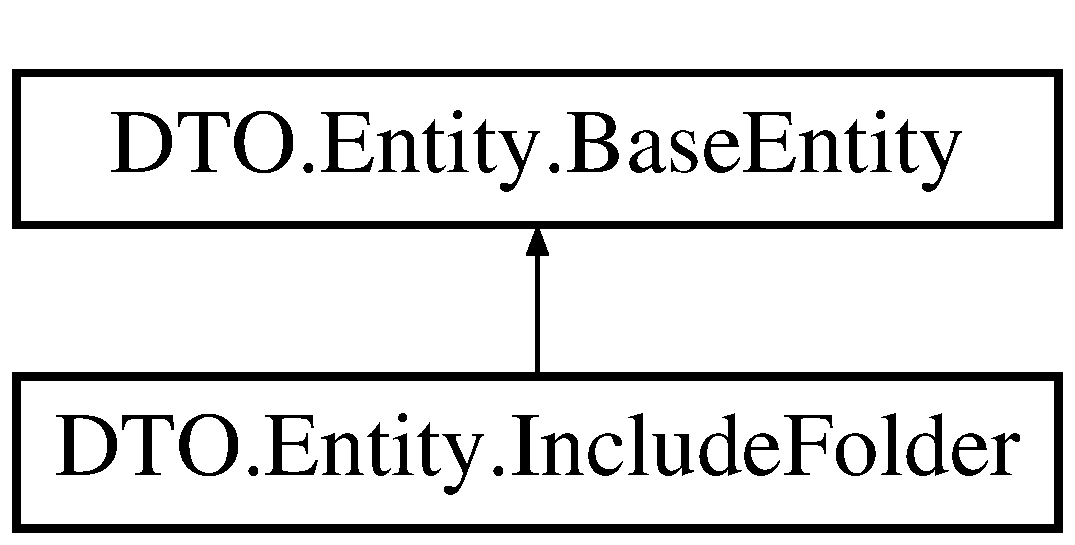
\includegraphics[height=2.000000cm]{class_d_t_o_1_1_entity_1_1_include_folder}
\end{center}
\end{figure}
\subsection*{Properties}
\begin{DoxyCompactItemize}
\item 
\mbox{\Hypertarget{class_d_t_o_1_1_entity_1_1_include_folder_a4a850b2a89d19e558bc14e224ad3c756}\label{class_d_t_o_1_1_entity_1_1_include_folder_a4a850b2a89d19e558bc14e224ad3c756}} 
string {\bfseries Path}\hspace{0.3cm}{\ttfamily  \mbox{[}get, set\mbox{]}}
\end{DoxyCompactItemize}


\subsection{Detailed Description}
The database \hyperlink{class_d_t_o_1_1_entity_1_1_include_folder}{Include\+Folder} entity 



The documentation for this class was generated from the following file\+:\begin{DoxyCompactItemize}
\item 
C\+:/\+W\+O\+R\+K\+S\+P\+A\+C\+E/\+T\+P\+I-\/end/\+Gestion\+Audio/\+D\+T\+O/\+Entity/Include\+Folder.\+cs\end{DoxyCompactItemize}

\hypertarget{class_presentation_1_1_converter_1_1_is_playing_image}{}\section{Presentation.\+Converter.\+Is\+Playing\+Image Class Reference}
\label{class_presentation_1_1_converter_1_1_is_playing_image}\index{Presentation.\+Converter.\+Is\+Playing\+Image@{Presentation.\+Converter.\+Is\+Playing\+Image}}


\hyperlink{namespace_presentation_1_1_converter}{Converter} used for the reading\+List\+View  


Inheritance diagram for Presentation.\+Converter.\+Is\+Playing\+Image\+:\begin{figure}[H]
\begin{center}
\leavevmode
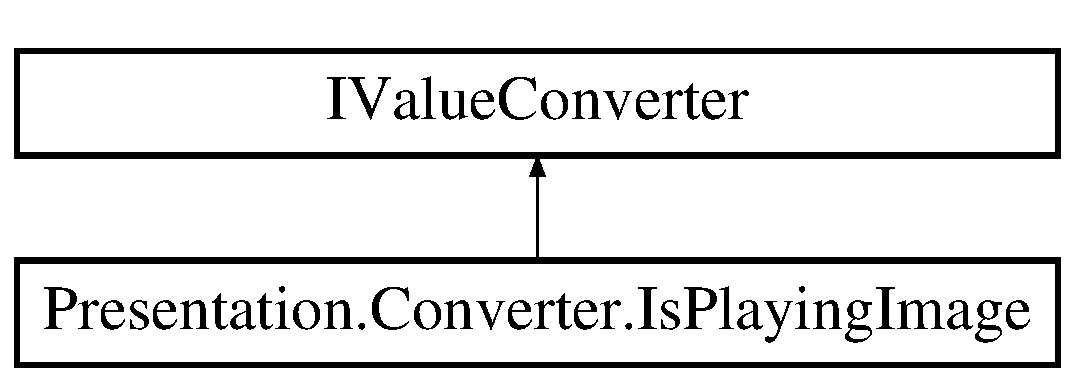
\includegraphics[height=2.000000cm]{class_presentation_1_1_converter_1_1_is_playing_image}
\end{center}
\end{figure}
\subsection*{Public Member Functions}
\begin{DoxyCompactItemize}
\item 
object \hyperlink{class_presentation_1_1_converter_1_1_is_playing_image_ab6d06255e3f26f1011d65b86d507a881}{Convert} (object value, Type target\+Type, object parameter, Culture\+Info culture)
\begin{DoxyCompactList}\small\item\em Display a picture of play if the music is acually playing \end{DoxyCompactList}\item 
\mbox{\Hypertarget{class_presentation_1_1_converter_1_1_is_playing_image_a14fcd97ce4a2cfd6eae063f7064f8e91}\label{class_presentation_1_1_converter_1_1_is_playing_image_a14fcd97ce4a2cfd6eae063f7064f8e91}} 
object {\bfseries Convert\+Back} (object value, Type target\+Type, object parameter, Culture\+Info culture)
\end{DoxyCompactItemize}


\subsection{Detailed Description}
\hyperlink{namespace_presentation_1_1_converter}{Converter} used for the reading\+List\+View 



\subsection{Member Function Documentation}
\mbox{\Hypertarget{class_presentation_1_1_converter_1_1_is_playing_image_ab6d06255e3f26f1011d65b86d507a881}\label{class_presentation_1_1_converter_1_1_is_playing_image_ab6d06255e3f26f1011d65b86d507a881}} 
\index{Presentation\+::\+Converter\+::\+Is\+Playing\+Image@{Presentation\+::\+Converter\+::\+Is\+Playing\+Image}!Convert@{Convert}}
\index{Convert@{Convert}!Presentation\+::\+Converter\+::\+Is\+Playing\+Image@{Presentation\+::\+Converter\+::\+Is\+Playing\+Image}}
\subsubsection{\texorpdfstring{Convert()}{Convert()}}
{\footnotesize\ttfamily object Presentation.\+Converter.\+Is\+Playing\+Image.\+Convert (\begin{DoxyParamCaption}\item[{object}]{value,  }\item[{Type}]{target\+Type,  }\item[{object}]{parameter,  }\item[{Culture\+Info}]{culture }\end{DoxyParamCaption})}



Display a picture of play if the music is acually playing 


\begin{DoxyParams}{Parameters}
{\em value} & \\
\hline
{\em target\+Type} & \\
\hline
{\em parameter} & \\
\hline
{\em culture} & \\
\hline
\end{DoxyParams}
\begin{DoxyReturn}{Returns}

\end{DoxyReturn}


The documentation for this class was generated from the following file\+:\begin{DoxyCompactItemize}
\item 
C\+:/\+W\+O\+R\+K\+S\+P\+A\+C\+E/\+T\+P\+I-\/end/\+Gestion\+Audio/\+Gestion\+Audio/\+Converter/Is\+Playing\+Image.\+cs\end{DoxyCompactItemize}

\hypertarget{class_presentation_1_1_view_model_1_1_main_view_model}{}\section{Presentation.\+View\+Model.\+Main\+View\+Model Class Reference}
\label{class_presentation_1_1_view_model_1_1_main_view_model}\index{Presentation.\+View\+Model.\+Main\+View\+Model@{Presentation.\+View\+Model.\+Main\+View\+Model}}


This class contains properties that the main \hyperlink{namespace_presentation_1_1_view}{View} can data bind to.  


Inheritance diagram for Presentation.\+View\+Model.\+Main\+View\+Model\+:\begin{figure}[H]
\begin{center}
\leavevmode
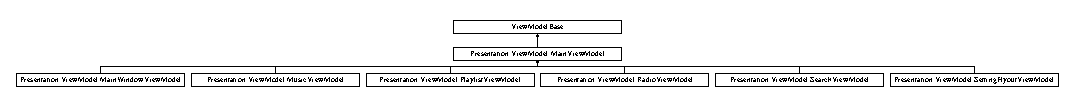
\includegraphics[height=0.942761cm]{class_presentation_1_1_view_model_1_1_main_view_model}
\end{center}
\end{figure}
\subsection*{Public Member Functions}
\begin{DoxyCompactItemize}
\item 
\hyperlink{class_presentation_1_1_view_model_1_1_main_view_model_a426844e65f93f554671ca046aec78eb3}{Main\+View\+Model} ()
\begin{DoxyCompactList}\small\item\em Initializes a new instance of the \hyperlink{class_presentation_1_1_view_model_1_1_main_view_model}{Main\+View\+Model} class. \end{DoxyCompactList}\end{DoxyCompactItemize}


\subsection{Detailed Description}
This class contains properties that the main \hyperlink{namespace_presentation_1_1_view}{View} can data bind to. 

Use the {\bfseries mvvminpc} snippet to add bindable properties to this \hyperlink{namespace_presentation_1_1_view_model}{View\+Model}. 

You can also use Blend to data bind with the tool\textquotesingle{}s support. 

See \href{http://www.galasoft.ch/mvvm}{\tt http\+://www.\+galasoft.\+ch/mvvm} 

\subsection{Constructor \& Destructor Documentation}
\mbox{\Hypertarget{class_presentation_1_1_view_model_1_1_main_view_model_a426844e65f93f554671ca046aec78eb3}\label{class_presentation_1_1_view_model_1_1_main_view_model_a426844e65f93f554671ca046aec78eb3}} 
\index{Presentation\+::\+View\+Model\+::\+Main\+View\+Model@{Presentation\+::\+View\+Model\+::\+Main\+View\+Model}!Main\+View\+Model@{Main\+View\+Model}}
\index{Main\+View\+Model@{Main\+View\+Model}!Presentation\+::\+View\+Model\+::\+Main\+View\+Model@{Presentation\+::\+View\+Model\+::\+Main\+View\+Model}}
\subsubsection{\texorpdfstring{Main\+View\+Model()}{MainViewModel()}}
{\footnotesize\ttfamily Presentation.\+View\+Model.\+Main\+View\+Model.\+Main\+View\+Model (\begin{DoxyParamCaption}{ }\end{DoxyParamCaption})}



Initializes a new instance of the \hyperlink{class_presentation_1_1_view_model_1_1_main_view_model}{Main\+View\+Model} class. 



The documentation for this class was generated from the following file\+:\begin{DoxyCompactItemize}
\item 
C\+:/\+W\+O\+R\+K\+S\+P\+A\+C\+E/\+T\+P\+I-\/end/\+Gestion\+Audio/\+Gestion\+Audio/\+View\+Model/Main\+View\+Model.\+cs\end{DoxyCompactItemize}

\hypertarget{class_presentation_1_1_main_window}{}\section{Presentation.\+Main\+Window Class Reference}
\label{class_presentation_1_1_main_window}\index{Presentation.\+Main\+Window@{Presentation.\+Main\+Window}}


Interaction logic for Main\+Window.\+xaml  


Inheritance diagram for Presentation.\+Main\+Window\+:\begin{figure}[H]
\begin{center}
\leavevmode
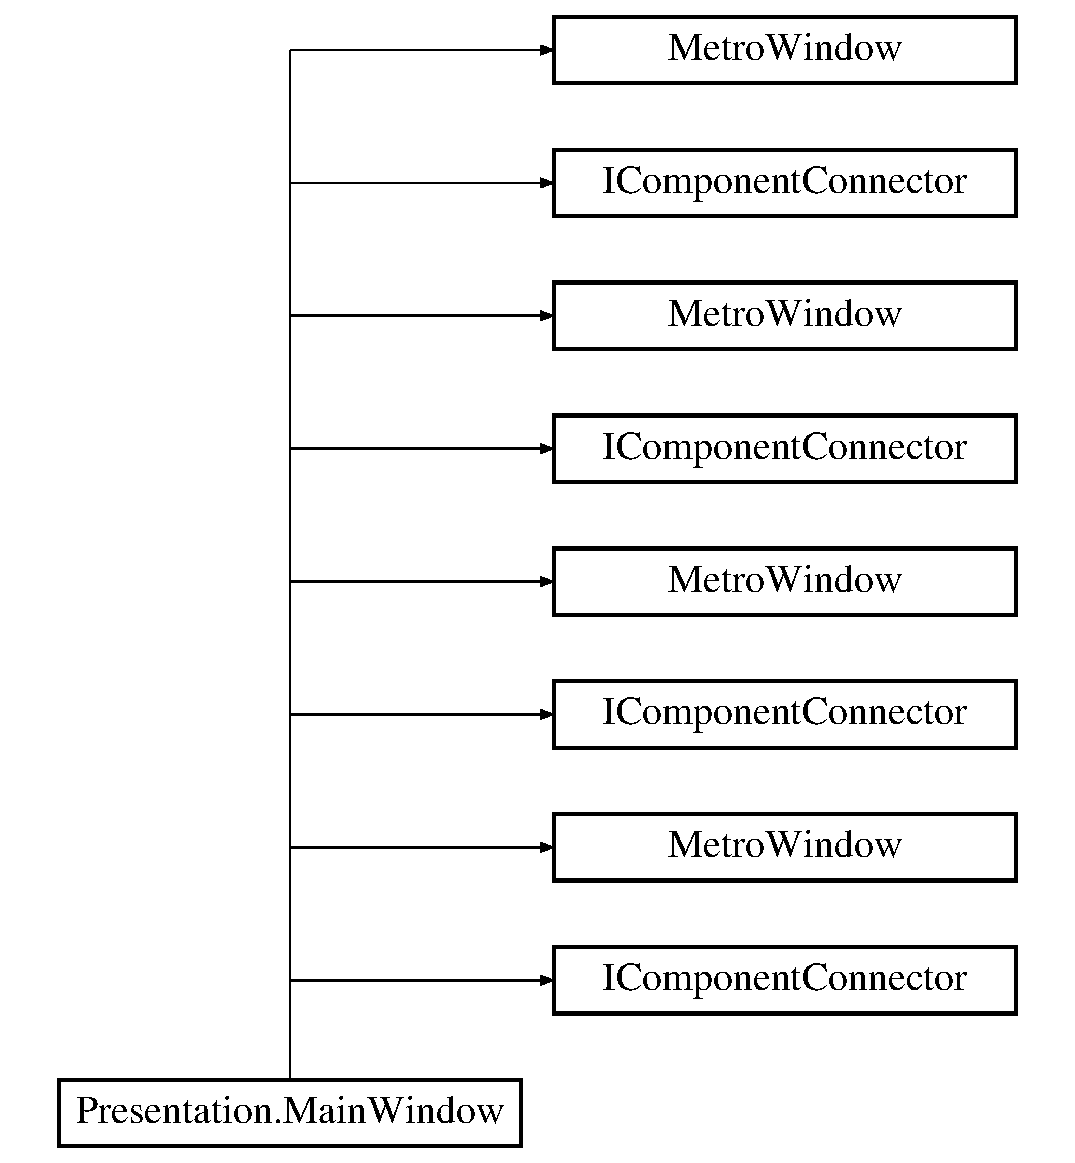
\includegraphics[height=9.000000cm]{class_presentation_1_1_main_window}
\end{center}
\end{figure}
\subsection*{Public Member Functions}
\begin{DoxyCompactItemize}
\item 
\hyperlink{class_presentation_1_1_main_window_a9f2c85f07c861da5f287d482913cc7f1}{Main\+Window} ()
\begin{DoxyCompactList}\small\item\em Set the good dll of C++runtime \end{DoxyCompactList}\item 
void \hyperlink{class_presentation_1_1_main_window_ae65bc3f86809be61714a19b6c8b9fba0}{Initialize\+Component} ()
\begin{DoxyCompactList}\small\item\em Initialize\+Component \end{DoxyCompactList}\item 
void \hyperlink{class_presentation_1_1_main_window_ae65bc3f86809be61714a19b6c8b9fba0}{Initialize\+Component} ()
\begin{DoxyCompactList}\small\item\em Initialize\+Component \end{DoxyCompactList}\item 
void \hyperlink{class_presentation_1_1_main_window_ae65bc3f86809be61714a19b6c8b9fba0}{Initialize\+Component} ()
\begin{DoxyCompactList}\small\item\em Initialize\+Component \end{DoxyCompactList}\item 
void \hyperlink{class_presentation_1_1_main_window_ae65bc3f86809be61714a19b6c8b9fba0}{Initialize\+Component} ()
\begin{DoxyCompactList}\small\item\em Initialize\+Component \end{DoxyCompactList}\end{DoxyCompactItemize}


\subsection{Detailed Description}
Interaction logic for Main\+Window.\+xaml 

\hyperlink{class_presentation_1_1_main_window}{Main\+Window} 

\subsection{Constructor \& Destructor Documentation}
\mbox{\Hypertarget{class_presentation_1_1_main_window_a9f2c85f07c861da5f287d482913cc7f1}\label{class_presentation_1_1_main_window_a9f2c85f07c861da5f287d482913cc7f1}} 
\index{Presentation\+::\+Main\+Window@{Presentation\+::\+Main\+Window}!Main\+Window@{Main\+Window}}
\index{Main\+Window@{Main\+Window}!Presentation\+::\+Main\+Window@{Presentation\+::\+Main\+Window}}
\subsubsection{\texorpdfstring{Main\+Window()}{MainWindow()}}
{\footnotesize\ttfamily Presentation.\+Main\+Window.\+Main\+Window (\begin{DoxyParamCaption}{ }\end{DoxyParamCaption})}



Set the good dll of C++runtime 



\subsection{Member Function Documentation}
\mbox{\Hypertarget{class_presentation_1_1_main_window_ae65bc3f86809be61714a19b6c8b9fba0}\label{class_presentation_1_1_main_window_ae65bc3f86809be61714a19b6c8b9fba0}} 
\index{Presentation\+::\+Main\+Window@{Presentation\+::\+Main\+Window}!Initialize\+Component@{Initialize\+Component}}
\index{Initialize\+Component@{Initialize\+Component}!Presentation\+::\+Main\+Window@{Presentation\+::\+Main\+Window}}
\subsubsection{\texorpdfstring{Initialize\+Component()}{InitializeComponent()}\hspace{0.1cm}{\footnotesize\ttfamily [1/4]}}
{\footnotesize\ttfamily void Presentation.\+Main\+Window.\+Initialize\+Component (\begin{DoxyParamCaption}{ }\end{DoxyParamCaption})}



Initialize\+Component 

\mbox{\Hypertarget{class_presentation_1_1_main_window_ae65bc3f86809be61714a19b6c8b9fba0}\label{class_presentation_1_1_main_window_ae65bc3f86809be61714a19b6c8b9fba0}} 
\index{Presentation\+::\+Main\+Window@{Presentation\+::\+Main\+Window}!Initialize\+Component@{Initialize\+Component}}
\index{Initialize\+Component@{Initialize\+Component}!Presentation\+::\+Main\+Window@{Presentation\+::\+Main\+Window}}
\subsubsection{\texorpdfstring{Initialize\+Component()}{InitializeComponent()}\hspace{0.1cm}{\footnotesize\ttfamily [2/4]}}
{\footnotesize\ttfamily void Presentation.\+Main\+Window.\+Initialize\+Component (\begin{DoxyParamCaption}{ }\end{DoxyParamCaption})}



Initialize\+Component 

\mbox{\Hypertarget{class_presentation_1_1_main_window_ae65bc3f86809be61714a19b6c8b9fba0}\label{class_presentation_1_1_main_window_ae65bc3f86809be61714a19b6c8b9fba0}} 
\index{Presentation\+::\+Main\+Window@{Presentation\+::\+Main\+Window}!Initialize\+Component@{Initialize\+Component}}
\index{Initialize\+Component@{Initialize\+Component}!Presentation\+::\+Main\+Window@{Presentation\+::\+Main\+Window}}
\subsubsection{\texorpdfstring{Initialize\+Component()}{InitializeComponent()}\hspace{0.1cm}{\footnotesize\ttfamily [3/4]}}
{\footnotesize\ttfamily void Presentation.\+Main\+Window.\+Initialize\+Component (\begin{DoxyParamCaption}{ }\end{DoxyParamCaption})}



Initialize\+Component 

\mbox{\Hypertarget{class_presentation_1_1_main_window_ae65bc3f86809be61714a19b6c8b9fba0}\label{class_presentation_1_1_main_window_ae65bc3f86809be61714a19b6c8b9fba0}} 
\index{Presentation\+::\+Main\+Window@{Presentation\+::\+Main\+Window}!Initialize\+Component@{Initialize\+Component}}
\index{Initialize\+Component@{Initialize\+Component}!Presentation\+::\+Main\+Window@{Presentation\+::\+Main\+Window}}
\subsubsection{\texorpdfstring{Initialize\+Component()}{InitializeComponent()}\hspace{0.1cm}{\footnotesize\ttfamily [4/4]}}
{\footnotesize\ttfamily void Presentation.\+Main\+Window.\+Initialize\+Component (\begin{DoxyParamCaption}{ }\end{DoxyParamCaption})}



Initialize\+Component 



The documentation for this class was generated from the following files\+:\begin{DoxyCompactItemize}
\item 
C\+:/\+W\+O\+R\+K\+S\+P\+A\+C\+E/\+T\+P\+I-\/end/\+Gestion\+Audio/\+Gestion\+Audio/Main\+Window.\+xaml.\+cs\item 
C\+:/\+W\+O\+R\+K\+S\+P\+A\+C\+E/\+T\+P\+I-\/end/\+Gestion\+Audio/\+Gestion\+Audio/obj/\+Debug/Main\+Window.\+g.\+cs\item 
C\+:/\+W\+O\+R\+K\+S\+P\+A\+C\+E/\+T\+P\+I-\/end/\+Gestion\+Audio/\+Gestion\+Audio/obj/\+Debug/Main\+Window.\+g.\+i.\+cs\end{DoxyCompactItemize}

\hypertarget{class_presentation_1_1_view_model_1_1_main_window_view_model}{}\section{Presentation.\+View\+Model.\+Main\+Window\+View\+Model Class Reference}
\label{class_presentation_1_1_view_model_1_1_main_window_view_model}\index{Presentation.\+View\+Model.\+Main\+Window\+View\+Model@{Presentation.\+View\+Model.\+Main\+Window\+View\+Model}}


\hyperlink{namespace_presentation_1_1_view_model}{View\+Model} to \hyperlink{class_presentation_1_1_main_window}{Main\+Window}  


Inheritance diagram for Presentation.\+View\+Model.\+Main\+Window\+View\+Model\+:\begin{figure}[H]
\begin{center}
\leavevmode
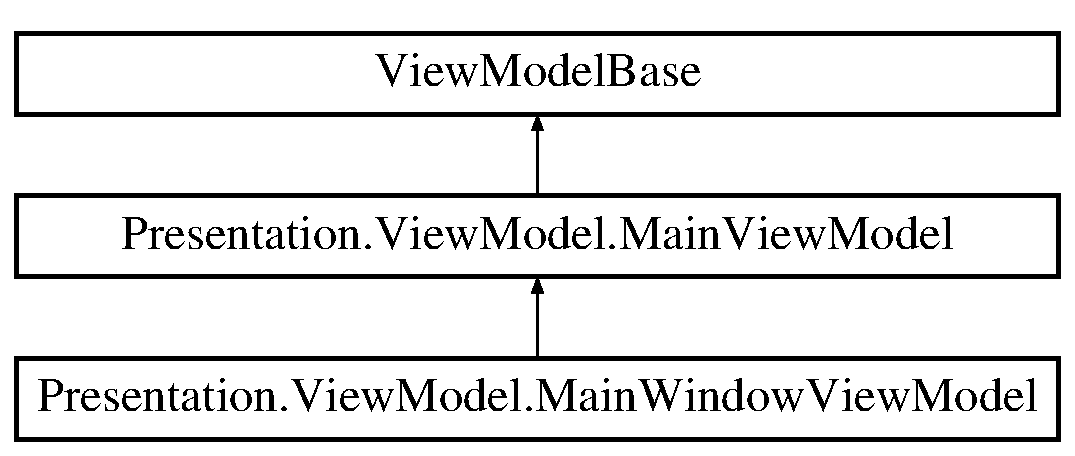
\includegraphics[height=3.000000cm]{class_presentation_1_1_view_model_1_1_main_window_view_model}
\end{center}
\end{figure}
\subsection*{Public Member Functions}
\begin{DoxyCompactItemize}
\item 
\hyperlink{class_presentation_1_1_view_model_1_1_main_window_view_model_a05bd3d883c2a4082b5d265f9c9b7e521}{Main\+Window\+View\+Model} ()
\begin{DoxyCompactList}\small\item\em Load all the relaycommands and chekc if there is no music \end{DoxyCompactList}\item 
void \hyperlink{class_presentation_1_1_view_model_1_1_main_window_view_model_ae0cd1aad0ab006978a0960a860a13c22}{Click\+Music} ()
\begin{DoxyCompactList}\small\item\em Open the music view \end{DoxyCompactList}\item 
void \hyperlink{class_presentation_1_1_view_model_1_1_main_window_view_model_a2758217be5d01273574939025c5ff937}{Click\+Playlist} ()
\begin{DoxyCompactList}\small\item\em Open the playlist view \end{DoxyCompactList}\item 
void \hyperlink{class_presentation_1_1_view_model_1_1_main_window_view_model_a62f6e4ed74af5d290ca6886d9dbf2a34}{Click\+Radio} ()
\begin{DoxyCompactList}\small\item\em Open the radio view \end{DoxyCompactList}\item 
void \hyperlink{class_presentation_1_1_view_model_1_1_main_window_view_model_a6dc7186d6c37dad719f22cc6e6b4efc8}{Save\+Context} ()
\begin{DoxyCompactList}\small\item\em Save the actual context \end{DoxyCompactList}\end{DoxyCompactItemize}
\subsection*{Static Public Attributes}
\begin{DoxyCompactItemize}
\item 
\mbox{\Hypertarget{class_presentation_1_1_view_model_1_1_main_window_view_model_a0c47ee3af00198ade201f6b4d847f104}\label{class_presentation_1_1_view_model_1_1_main_window_view_model_a0c47ee3af00198ade201f6b4d847f104}} 
static \hyperlink{class_presentation_1_1_view_model_1_1_main_window_view_model}{Main\+Window\+View\+Model} {\bfseries Main}
\item 
\mbox{\Hypertarget{class_presentation_1_1_view_model_1_1_main_window_view_model_a8380e5ea810180a647ecdbb8048a92c6}\label{class_presentation_1_1_view_model_1_1_main_window_view_model_a8380e5ea810180a647ecdbb8048a92c6}} 
static Metro\+Window {\bfseries Metro\+Window} = (System.\+Windows.\+Application.\+Current.\+Main\+Window as Metro\+Window)
\end{DoxyCompactItemize}
\subsection*{Properties}
\begin{DoxyCompactItemize}
\item 
\mbox{\Hypertarget{class_presentation_1_1_view_model_1_1_main_window_view_model_a11e5d71c56b3e66443283e661887af8d}\label{class_presentation_1_1_view_model_1_1_main_window_view_model_a11e5d71c56b3e66443283e661887af8d}} 
Relay\+Command {\bfseries On\+Close}\hspace{0.3cm}{\ttfamily  \mbox{[}get, set\mbox{]}}
\item 
\mbox{\Hypertarget{class_presentation_1_1_view_model_1_1_main_window_view_model_a983f81992ec0080d08aabdb79db226e4}\label{class_presentation_1_1_view_model_1_1_main_window_view_model_a983f81992ec0080d08aabdb79db226e4}} 
static \hyperlink{class_presentation_1_1_view_model_1_1_player_view_model}{Player\+View\+Model} {\bfseries Player\+View\+Model}\hspace{0.3cm}{\ttfamily  \mbox{[}get, set\mbox{]}}
\item 
\mbox{\Hypertarget{class_presentation_1_1_view_model_1_1_main_window_view_model_ab04bb7bf8826492079602556a7fbc2a7}\label{class_presentation_1_1_view_model_1_1_main_window_view_model_ab04bb7bf8826492079602556a7fbc2a7}} 
User\+Control {\bfseries Actual\+View} = new \hyperlink{class_presentation_1_1_view_model_1_1_player_view_model}{Player\+View\+Model}()\hspace{0.3cm}{\ttfamily  \mbox{[}get, set\mbox{]}}
\item 
\mbox{\Hypertarget{class_presentation_1_1_view_model_1_1_main_window_view_model_ab01da93fe0f1336bf118f0b4c72ecc11}\label{class_presentation_1_1_view_model_1_1_main_window_view_model_ab01da93fe0f1336bf118f0b4c72ecc11}} 
string {\bfseries Analyse\+Status}\hspace{0.3cm}{\ttfamily  \mbox{[}get, set\mbox{]}}
\item 
\mbox{\Hypertarget{class_presentation_1_1_view_model_1_1_main_window_view_model_a4fc2203dbc2da6ae275e8a03b578e89f}\label{class_presentation_1_1_view_model_1_1_main_window_view_model_a4fc2203dbc2da6ae275e8a03b578e89f}} 
bool {\bfseries Is\+Flyout\+Music\+Open}\hspace{0.3cm}{\ttfamily  \mbox{[}get, set\mbox{]}}
\item 
\mbox{\Hypertarget{class_presentation_1_1_view_model_1_1_main_window_view_model_aef904bfcbd0bf9213b226789921196e3}\label{class_presentation_1_1_view_model_1_1_main_window_view_model_aef904bfcbd0bf9213b226789921196e3}} 
bool {\bfseries Is\+Flyout\+Reading\+List\+Open}\hspace{0.3cm}{\ttfamily  \mbox{[}get, set\mbox{]}}
\item 
\mbox{\Hypertarget{class_presentation_1_1_view_model_1_1_main_window_view_model_aaa239b46f39f79378a055aedb375f423}\label{class_presentation_1_1_view_model_1_1_main_window_view_model_aaa239b46f39f79378a055aedb375f423}} 
bool {\bfseries Is\+Flyout\+Running\+Open}\hspace{0.3cm}{\ttfamily  \mbox{[}get, set\mbox{]}}
\item 
\mbox{\Hypertarget{class_presentation_1_1_view_model_1_1_main_window_view_model_a3776bac08386524ca3e5ca41810e21df}\label{class_presentation_1_1_view_model_1_1_main_window_view_model_a3776bac08386524ca3e5ca41810e21df}} 
bool {\bfseries Is\+Flyout\+Setting\+Open}\hspace{0.3cm}{\ttfamily  \mbox{[}get, set\mbox{]}}
\item 
\mbox{\Hypertarget{class_presentation_1_1_view_model_1_1_main_window_view_model_a3a4b5516c20e3d8ad2e33050cf730011}\label{class_presentation_1_1_view_model_1_1_main_window_view_model_a3a4b5516c20e3d8ad2e33050cf730011}} 
\hyperlink{class_presentation_1_1_view_model_1_1_music_view_model}{Music\+View\+Model} {\bfseries Music\+View\+Model}\hspace{0.3cm}{\ttfamily  \mbox{[}get, set\mbox{]}}
\item 
\mbox{\Hypertarget{class_presentation_1_1_view_model_1_1_main_window_view_model_ab239bf8dd6b995e466036291e3c8c38e}\label{class_presentation_1_1_view_model_1_1_main_window_view_model_ab239bf8dd6b995e466036291e3c8c38e}} 
Relay\+Command {\bfseries On\+Click\+Element}\hspace{0.3cm}{\ttfamily  \mbox{[}get, set\mbox{]}}
\item 
\mbox{\Hypertarget{class_presentation_1_1_view_model_1_1_main_window_view_model_a6e0aa7f847de771f9d996699be5a2e09}\label{class_presentation_1_1_view_model_1_1_main_window_view_model_a6e0aa7f847de771f9d996699be5a2e09}} 
Relay\+Command {\bfseries On\+Click\+Music}\hspace{0.3cm}{\ttfamily  \mbox{[}get, set\mbox{]}}
\item 
\mbox{\Hypertarget{class_presentation_1_1_view_model_1_1_main_window_view_model_a895c59669eb67d5fb90ddfa18549a808}\label{class_presentation_1_1_view_model_1_1_main_window_view_model_a895c59669eb67d5fb90ddfa18549a808}} 
Relay\+Command {\bfseries On\+Click\+Playlist}\hspace{0.3cm}{\ttfamily  \mbox{[}get, set\mbox{]}}
\item 
\mbox{\Hypertarget{class_presentation_1_1_view_model_1_1_main_window_view_model_afc39702e8a5f2ee4cda1b47d56804357}\label{class_presentation_1_1_view_model_1_1_main_window_view_model_afc39702e8a5f2ee4cda1b47d56804357}} 
Relay\+Command {\bfseries On\+Click\+Radio}\hspace{0.3cm}{\ttfamily  \mbox{[}get, set\mbox{]}}
\item 
\mbox{\Hypertarget{class_presentation_1_1_view_model_1_1_main_window_view_model_ac514a5d3b4d7798f0e672454c5b252ca}\label{class_presentation_1_1_view_model_1_1_main_window_view_model_ac514a5d3b4d7798f0e672454c5b252ca}} 
Relay\+Command {\bfseries On\+Open\+Setting\+Flyout}\hspace{0.3cm}{\ttfamily  \mbox{[}get, set\mbox{]}}
\item 
\mbox{\Hypertarget{class_presentation_1_1_view_model_1_1_main_window_view_model_a213bdaf63e15042cd2f8516c72a2e8b3}\label{class_presentation_1_1_view_model_1_1_main_window_view_model_a213bdaf63e15042cd2f8516c72a2e8b3}} 
Relay\+Command {\bfseries On\+Search}\hspace{0.3cm}{\ttfamily  \mbox{[}get, set\mbox{]}}
\item 
\mbox{\Hypertarget{class_presentation_1_1_view_model_1_1_main_window_view_model_af8966ce8dd01aae5d65132b09320be95}\label{class_presentation_1_1_view_model_1_1_main_window_view_model_af8966ce8dd01aae5d65132b09320be95}} 
Observable\+Collection$<$ \hyperlink{class_d_t_o_1_1_entity_1_1_track}{Track} $>$ {\bfseries Reading\+List}\hspace{0.3cm}{\ttfamily  \mbox{[}get, set\mbox{]}}
\item 
\mbox{\Hypertarget{class_presentation_1_1_view_model_1_1_main_window_view_model_acba73ffb81d8d077dfc007528d074979}\label{class_presentation_1_1_view_model_1_1_main_window_view_model_acba73ffb81d8d077dfc007528d074979}} 
string {\bfseries Search\+Text}\hspace{0.3cm}{\ttfamily  \mbox{[}get, set\mbox{]}}
\item 
\hyperlink{class_d_t_o_1_1_entity_1_1_track}{Track} \hyperlink{class_presentation_1_1_view_model_1_1_main_window_view_model_a0cafef1627d04f131f5541b30225018a}{Selected\+Item}\hspace{0.3cm}{\ttfamily  \mbox{[}get, set\mbox{]}}
\begin{DoxyCompactList}\small\item\em The selected track of the reading list \end{DoxyCompactList}\item 
\mbox{\Hypertarget{class_presentation_1_1_view_model_1_1_main_window_view_model_ab7e5452844ea79cae2829cbe1dddbfbd}\label{class_presentation_1_1_view_model_1_1_main_window_view_model_ab7e5452844ea79cae2829cbe1dddbfbd}} 
\hyperlink{class_presentation_1_1_view_model_1_1_setting_flyout_view_model}{Setting\+Flyout\+View\+Model} {\bfseries Setting\+Flyout\+View\+Model}\hspace{0.3cm}{\ttfamily  \mbox{[}get, set\mbox{]}}
\end{DoxyCompactItemize}


\subsection{Detailed Description}
\hyperlink{namespace_presentation_1_1_view_model}{View\+Model} to \hyperlink{class_presentation_1_1_main_window}{Main\+Window} 



\subsection{Constructor \& Destructor Documentation}
\mbox{\Hypertarget{class_presentation_1_1_view_model_1_1_main_window_view_model_a05bd3d883c2a4082b5d265f9c9b7e521}\label{class_presentation_1_1_view_model_1_1_main_window_view_model_a05bd3d883c2a4082b5d265f9c9b7e521}} 
\index{Presentation\+::\+View\+Model\+::\+Main\+Window\+View\+Model@{Presentation\+::\+View\+Model\+::\+Main\+Window\+View\+Model}!Main\+Window\+View\+Model@{Main\+Window\+View\+Model}}
\index{Main\+Window\+View\+Model@{Main\+Window\+View\+Model}!Presentation\+::\+View\+Model\+::\+Main\+Window\+View\+Model@{Presentation\+::\+View\+Model\+::\+Main\+Window\+View\+Model}}
\subsubsection{\texorpdfstring{Main\+Window\+View\+Model()}{MainWindowViewModel()}}
{\footnotesize\ttfamily Presentation.\+View\+Model.\+Main\+Window\+View\+Model.\+Main\+Window\+View\+Model (\begin{DoxyParamCaption}{ }\end{DoxyParamCaption})}



Load all the relaycommands and chekc if there is no music 



\subsection{Member Function Documentation}
\mbox{\Hypertarget{class_presentation_1_1_view_model_1_1_main_window_view_model_ae0cd1aad0ab006978a0960a860a13c22}\label{class_presentation_1_1_view_model_1_1_main_window_view_model_ae0cd1aad0ab006978a0960a860a13c22}} 
\index{Presentation\+::\+View\+Model\+::\+Main\+Window\+View\+Model@{Presentation\+::\+View\+Model\+::\+Main\+Window\+View\+Model}!Click\+Music@{Click\+Music}}
\index{Click\+Music@{Click\+Music}!Presentation\+::\+View\+Model\+::\+Main\+Window\+View\+Model@{Presentation\+::\+View\+Model\+::\+Main\+Window\+View\+Model}}
\subsubsection{\texorpdfstring{Click\+Music()}{ClickMusic()}}
{\footnotesize\ttfamily void Presentation.\+View\+Model.\+Main\+Window\+View\+Model.\+Click\+Music (\begin{DoxyParamCaption}{ }\end{DoxyParamCaption})}



Open the music view 

\mbox{\Hypertarget{class_presentation_1_1_view_model_1_1_main_window_view_model_a2758217be5d01273574939025c5ff937}\label{class_presentation_1_1_view_model_1_1_main_window_view_model_a2758217be5d01273574939025c5ff937}} 
\index{Presentation\+::\+View\+Model\+::\+Main\+Window\+View\+Model@{Presentation\+::\+View\+Model\+::\+Main\+Window\+View\+Model}!Click\+Playlist@{Click\+Playlist}}
\index{Click\+Playlist@{Click\+Playlist}!Presentation\+::\+View\+Model\+::\+Main\+Window\+View\+Model@{Presentation\+::\+View\+Model\+::\+Main\+Window\+View\+Model}}
\subsubsection{\texorpdfstring{Click\+Playlist()}{ClickPlaylist()}}
{\footnotesize\ttfamily void Presentation.\+View\+Model.\+Main\+Window\+View\+Model.\+Click\+Playlist (\begin{DoxyParamCaption}{ }\end{DoxyParamCaption})}



Open the playlist view 

\mbox{\Hypertarget{class_presentation_1_1_view_model_1_1_main_window_view_model_a62f6e4ed74af5d290ca6886d9dbf2a34}\label{class_presentation_1_1_view_model_1_1_main_window_view_model_a62f6e4ed74af5d290ca6886d9dbf2a34}} 
\index{Presentation\+::\+View\+Model\+::\+Main\+Window\+View\+Model@{Presentation\+::\+View\+Model\+::\+Main\+Window\+View\+Model}!Click\+Radio@{Click\+Radio}}
\index{Click\+Radio@{Click\+Radio}!Presentation\+::\+View\+Model\+::\+Main\+Window\+View\+Model@{Presentation\+::\+View\+Model\+::\+Main\+Window\+View\+Model}}
\subsubsection{\texorpdfstring{Click\+Radio()}{ClickRadio()}}
{\footnotesize\ttfamily void Presentation.\+View\+Model.\+Main\+Window\+View\+Model.\+Click\+Radio (\begin{DoxyParamCaption}{ }\end{DoxyParamCaption})}



Open the radio view 

\mbox{\Hypertarget{class_presentation_1_1_view_model_1_1_main_window_view_model_a6dc7186d6c37dad719f22cc6e6b4efc8}\label{class_presentation_1_1_view_model_1_1_main_window_view_model_a6dc7186d6c37dad719f22cc6e6b4efc8}} 
\index{Presentation\+::\+View\+Model\+::\+Main\+Window\+View\+Model@{Presentation\+::\+View\+Model\+::\+Main\+Window\+View\+Model}!Save\+Context@{Save\+Context}}
\index{Save\+Context@{Save\+Context}!Presentation\+::\+View\+Model\+::\+Main\+Window\+View\+Model@{Presentation\+::\+View\+Model\+::\+Main\+Window\+View\+Model}}
\subsubsection{\texorpdfstring{Save\+Context()}{SaveContext()}}
{\footnotesize\ttfamily void Presentation.\+View\+Model.\+Main\+Window\+View\+Model.\+Save\+Context (\begin{DoxyParamCaption}{ }\end{DoxyParamCaption})}



Save the actual context 



\subsection{Property Documentation}
\mbox{\Hypertarget{class_presentation_1_1_view_model_1_1_main_window_view_model_a0cafef1627d04f131f5541b30225018a}\label{class_presentation_1_1_view_model_1_1_main_window_view_model_a0cafef1627d04f131f5541b30225018a}} 
\index{Presentation\+::\+View\+Model\+::\+Main\+Window\+View\+Model@{Presentation\+::\+View\+Model\+::\+Main\+Window\+View\+Model}!Selected\+Item@{Selected\+Item}}
\index{Selected\+Item@{Selected\+Item}!Presentation\+::\+View\+Model\+::\+Main\+Window\+View\+Model@{Presentation\+::\+View\+Model\+::\+Main\+Window\+View\+Model}}
\subsubsection{\texorpdfstring{Selected\+Item}{SelectedItem}}
{\footnotesize\ttfamily \hyperlink{class_d_t_o_1_1_entity_1_1_track}{Track} Presentation.\+View\+Model.\+Main\+Window\+View\+Model.\+Selected\+Item\hspace{0.3cm}{\ttfamily [get]}, {\ttfamily [set]}}



The selected track of the reading list 



The documentation for this class was generated from the following file\+:\begin{DoxyCompactItemize}
\item 
C\+:/\+W\+O\+R\+K\+S\+P\+A\+C\+E/\+T\+P\+I-\/end/\+Gestion\+Audio/\+Gestion\+Audio/\+View\+Model/Main\+Window\+View\+Model.\+cs\end{DoxyCompactItemize}

\hypertarget{class_presentation_1_1_view_1_1_flyout_1_1_music_flyout_view}{}\section{Presentation.\+View.\+Flyout.\+Music\+Flyout\+View Class Reference}
\label{class_presentation_1_1_view_1_1_flyout_1_1_music_flyout_view}\index{Presentation.\+View.\+Flyout.\+Music\+Flyout\+View@{Presentation.\+View.\+Flyout.\+Music\+Flyout\+View}}


\hyperlink{class_presentation_1_1_view_1_1_flyout_1_1_music_flyout_view}{Music\+Flyout\+View}  


Inheritance diagram for Presentation.\+View.\+Flyout.\+Music\+Flyout\+View\+:\begin{figure}[H]
\begin{center}
\leavevmode
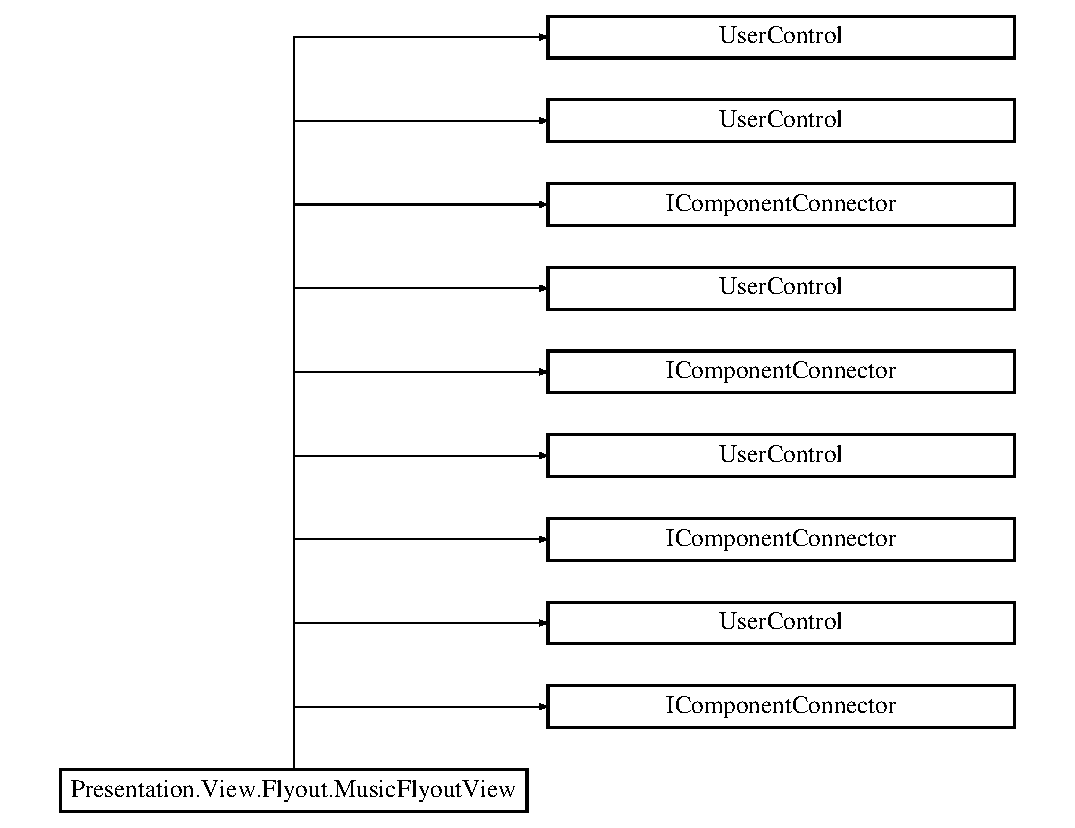
\includegraphics[height=10.000000cm]{class_presentation_1_1_view_1_1_flyout_1_1_music_flyout_view}
\end{center}
\end{figure}
\subsection*{Public Member Functions}
\begin{DoxyCompactItemize}
\item 
void \hyperlink{class_presentation_1_1_view_1_1_flyout_1_1_music_flyout_view_ae8007344b032def03546b7eed13aebef}{Initialize\+Component} ()
\begin{DoxyCompactList}\small\item\em Initialize\+Component \end{DoxyCompactList}\item 
void \hyperlink{class_presentation_1_1_view_1_1_flyout_1_1_music_flyout_view_ae8007344b032def03546b7eed13aebef}{Initialize\+Component} ()
\begin{DoxyCompactList}\small\item\em Initialize\+Component \end{DoxyCompactList}\item 
void \hyperlink{class_presentation_1_1_view_1_1_flyout_1_1_music_flyout_view_ae8007344b032def03546b7eed13aebef}{Initialize\+Component} ()
\begin{DoxyCompactList}\small\item\em Initialize\+Component \end{DoxyCompactList}\item 
void \hyperlink{class_presentation_1_1_view_1_1_flyout_1_1_music_flyout_view_ae8007344b032def03546b7eed13aebef}{Initialize\+Component} ()
\begin{DoxyCompactList}\small\item\em Initialize\+Component \end{DoxyCompactList}\end{DoxyCompactItemize}


\subsection{Detailed Description}
\hyperlink{class_presentation_1_1_view_1_1_flyout_1_1_music_flyout_view}{Music\+Flyout\+View} 

Interaction logic for Setting\+Flyout\+View.\+xaml 

\subsection{Member Function Documentation}
\mbox{\Hypertarget{class_presentation_1_1_view_1_1_flyout_1_1_music_flyout_view_ae8007344b032def03546b7eed13aebef}\label{class_presentation_1_1_view_1_1_flyout_1_1_music_flyout_view_ae8007344b032def03546b7eed13aebef}} 
\index{Presentation\+::\+View\+::\+Flyout\+::\+Music\+Flyout\+View@{Presentation\+::\+View\+::\+Flyout\+::\+Music\+Flyout\+View}!Initialize\+Component@{Initialize\+Component}}
\index{Initialize\+Component@{Initialize\+Component}!Presentation\+::\+View\+::\+Flyout\+::\+Music\+Flyout\+View@{Presentation\+::\+View\+::\+Flyout\+::\+Music\+Flyout\+View}}
\subsubsection{\texorpdfstring{Initialize\+Component()}{InitializeComponent()}\hspace{0.1cm}{\footnotesize\ttfamily [1/4]}}
{\footnotesize\ttfamily void Presentation.\+View.\+Flyout.\+Music\+Flyout\+View.\+Initialize\+Component (\begin{DoxyParamCaption}{ }\end{DoxyParamCaption})}



Initialize\+Component 

\mbox{\Hypertarget{class_presentation_1_1_view_1_1_flyout_1_1_music_flyout_view_ae8007344b032def03546b7eed13aebef}\label{class_presentation_1_1_view_1_1_flyout_1_1_music_flyout_view_ae8007344b032def03546b7eed13aebef}} 
\index{Presentation\+::\+View\+::\+Flyout\+::\+Music\+Flyout\+View@{Presentation\+::\+View\+::\+Flyout\+::\+Music\+Flyout\+View}!Initialize\+Component@{Initialize\+Component}}
\index{Initialize\+Component@{Initialize\+Component}!Presentation\+::\+View\+::\+Flyout\+::\+Music\+Flyout\+View@{Presentation\+::\+View\+::\+Flyout\+::\+Music\+Flyout\+View}}
\subsubsection{\texorpdfstring{Initialize\+Component()}{InitializeComponent()}\hspace{0.1cm}{\footnotesize\ttfamily [2/4]}}
{\footnotesize\ttfamily void Presentation.\+View.\+Flyout.\+Music\+Flyout\+View.\+Initialize\+Component (\begin{DoxyParamCaption}{ }\end{DoxyParamCaption})}



Initialize\+Component 

\mbox{\Hypertarget{class_presentation_1_1_view_1_1_flyout_1_1_music_flyout_view_ae8007344b032def03546b7eed13aebef}\label{class_presentation_1_1_view_1_1_flyout_1_1_music_flyout_view_ae8007344b032def03546b7eed13aebef}} 
\index{Presentation\+::\+View\+::\+Flyout\+::\+Music\+Flyout\+View@{Presentation\+::\+View\+::\+Flyout\+::\+Music\+Flyout\+View}!Initialize\+Component@{Initialize\+Component}}
\index{Initialize\+Component@{Initialize\+Component}!Presentation\+::\+View\+::\+Flyout\+::\+Music\+Flyout\+View@{Presentation\+::\+View\+::\+Flyout\+::\+Music\+Flyout\+View}}
\subsubsection{\texorpdfstring{Initialize\+Component()}{InitializeComponent()}\hspace{0.1cm}{\footnotesize\ttfamily [3/4]}}
{\footnotesize\ttfamily void Presentation.\+View.\+Flyout.\+Music\+Flyout\+View.\+Initialize\+Component (\begin{DoxyParamCaption}{ }\end{DoxyParamCaption})}



Initialize\+Component 

\mbox{\Hypertarget{class_presentation_1_1_view_1_1_flyout_1_1_music_flyout_view_ae8007344b032def03546b7eed13aebef}\label{class_presentation_1_1_view_1_1_flyout_1_1_music_flyout_view_ae8007344b032def03546b7eed13aebef}} 
\index{Presentation\+::\+View\+::\+Flyout\+::\+Music\+Flyout\+View@{Presentation\+::\+View\+::\+Flyout\+::\+Music\+Flyout\+View}!Initialize\+Component@{Initialize\+Component}}
\index{Initialize\+Component@{Initialize\+Component}!Presentation\+::\+View\+::\+Flyout\+::\+Music\+Flyout\+View@{Presentation\+::\+View\+::\+Flyout\+::\+Music\+Flyout\+View}}
\subsubsection{\texorpdfstring{Initialize\+Component()}{InitializeComponent()}\hspace{0.1cm}{\footnotesize\ttfamily [4/4]}}
{\footnotesize\ttfamily void Presentation.\+View.\+Flyout.\+Music\+Flyout\+View.\+Initialize\+Component (\begin{DoxyParamCaption}{ }\end{DoxyParamCaption})}



Initialize\+Component 



The documentation for this class was generated from the following files\+:\begin{DoxyCompactItemize}
\item 
C\+:/\+W\+O\+R\+K\+S\+P\+A\+C\+E/\+T\+P\+I-\/end/\+Gestion\+Audio/\+Gestion\+Audio/obj/\+Debug/\+View/\+Flyout/Music\+Flyout\+View.\+g.\+cs\item 
C\+:/\+W\+O\+R\+K\+S\+P\+A\+C\+E/\+T\+P\+I-\/end/\+Gestion\+Audio/\+Gestion\+Audio/obj/\+Debug/\+View/\+Flyout/Music\+Flyout\+View.\+g.\+i.\+cs\item 
C\+:/\+W\+O\+R\+K\+S\+P\+A\+C\+E/\+T\+P\+I-\/end/\+Gestion\+Audio/\+Gestion\+Audio/\+View/\+Flyout/Music\+Flyout\+View.\+xaml.\+cs\end{DoxyCompactItemize}

\hypertarget{class_presentation_1_1_view_1_1_music_view}{}\section{Presentation.\+View.\+Music\+View Class Reference}
\label{class_presentation_1_1_view_1_1_music_view}\index{Presentation.\+View.\+Music\+View@{Presentation.\+View.\+Music\+View}}


\hyperlink{class_presentation_1_1_view_1_1_music_view}{Music\+View}  


Inheritance diagram for Presentation.\+View.\+Music\+View\+:\begin{figure}[H]
\begin{center}
\leavevmode
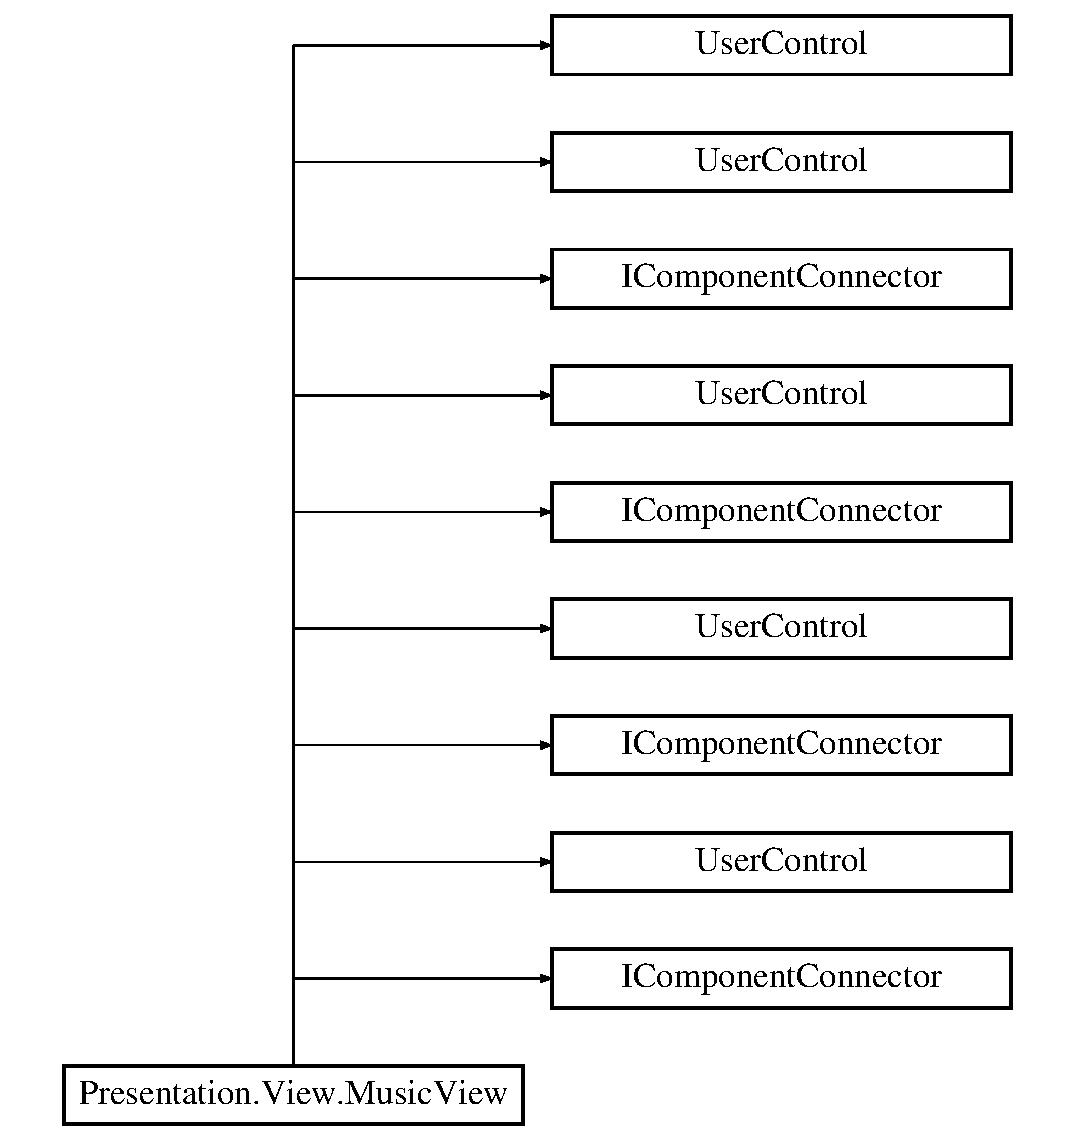
\includegraphics[height=10.000000cm]{class_presentation_1_1_view_1_1_music_view}
\end{center}
\end{figure}
\subsection*{Public Member Functions}
\begin{DoxyCompactItemize}
\item 
void \hyperlink{class_presentation_1_1_view_1_1_music_view_ad544f1791f3fd9b81adde25bbc9a90cf}{Initialize\+Component} ()
\begin{DoxyCompactList}\small\item\em Initialize\+Component \end{DoxyCompactList}\item 
void \hyperlink{class_presentation_1_1_view_1_1_music_view_ad544f1791f3fd9b81adde25bbc9a90cf}{Initialize\+Component} ()
\begin{DoxyCompactList}\small\item\em Initialize\+Component \end{DoxyCompactList}\item 
void \hyperlink{class_presentation_1_1_view_1_1_music_view_ad544f1791f3fd9b81adde25bbc9a90cf}{Initialize\+Component} ()
\begin{DoxyCompactList}\small\item\em Initialize\+Component \end{DoxyCompactList}\item 
void \hyperlink{class_presentation_1_1_view_1_1_music_view_ad544f1791f3fd9b81adde25bbc9a90cf}{Initialize\+Component} ()
\begin{DoxyCompactList}\small\item\em Initialize\+Component \end{DoxyCompactList}\end{DoxyCompactItemize}


\subsection{Detailed Description}
\hyperlink{class_presentation_1_1_view_1_1_music_view}{Music\+View} 

Interaction logic for Music\+View.\+xaml 

\subsection{Member Function Documentation}
\mbox{\Hypertarget{class_presentation_1_1_view_1_1_music_view_ad544f1791f3fd9b81adde25bbc9a90cf}\label{class_presentation_1_1_view_1_1_music_view_ad544f1791f3fd9b81adde25bbc9a90cf}} 
\index{Presentation\+::\+View\+::\+Music\+View@{Presentation\+::\+View\+::\+Music\+View}!Initialize\+Component@{Initialize\+Component}}
\index{Initialize\+Component@{Initialize\+Component}!Presentation\+::\+View\+::\+Music\+View@{Presentation\+::\+View\+::\+Music\+View}}
\subsubsection{\texorpdfstring{Initialize\+Component()}{InitializeComponent()}\hspace{0.1cm}{\footnotesize\ttfamily [1/4]}}
{\footnotesize\ttfamily void Presentation.\+View.\+Music\+View.\+Initialize\+Component (\begin{DoxyParamCaption}{ }\end{DoxyParamCaption})}



Initialize\+Component 

\mbox{\Hypertarget{class_presentation_1_1_view_1_1_music_view_ad544f1791f3fd9b81adde25bbc9a90cf}\label{class_presentation_1_1_view_1_1_music_view_ad544f1791f3fd9b81adde25bbc9a90cf}} 
\index{Presentation\+::\+View\+::\+Music\+View@{Presentation\+::\+View\+::\+Music\+View}!Initialize\+Component@{Initialize\+Component}}
\index{Initialize\+Component@{Initialize\+Component}!Presentation\+::\+View\+::\+Music\+View@{Presentation\+::\+View\+::\+Music\+View}}
\subsubsection{\texorpdfstring{Initialize\+Component()}{InitializeComponent()}\hspace{0.1cm}{\footnotesize\ttfamily [2/4]}}
{\footnotesize\ttfamily void Presentation.\+View.\+Music\+View.\+Initialize\+Component (\begin{DoxyParamCaption}{ }\end{DoxyParamCaption})}



Initialize\+Component 

\mbox{\Hypertarget{class_presentation_1_1_view_1_1_music_view_ad544f1791f3fd9b81adde25bbc9a90cf}\label{class_presentation_1_1_view_1_1_music_view_ad544f1791f3fd9b81adde25bbc9a90cf}} 
\index{Presentation\+::\+View\+::\+Music\+View@{Presentation\+::\+View\+::\+Music\+View}!Initialize\+Component@{Initialize\+Component}}
\index{Initialize\+Component@{Initialize\+Component}!Presentation\+::\+View\+::\+Music\+View@{Presentation\+::\+View\+::\+Music\+View}}
\subsubsection{\texorpdfstring{Initialize\+Component()}{InitializeComponent()}\hspace{0.1cm}{\footnotesize\ttfamily [3/4]}}
{\footnotesize\ttfamily void Presentation.\+View.\+Music\+View.\+Initialize\+Component (\begin{DoxyParamCaption}{ }\end{DoxyParamCaption})}



Initialize\+Component 

\mbox{\Hypertarget{class_presentation_1_1_view_1_1_music_view_ad544f1791f3fd9b81adde25bbc9a90cf}\label{class_presentation_1_1_view_1_1_music_view_ad544f1791f3fd9b81adde25bbc9a90cf}} 
\index{Presentation\+::\+View\+::\+Music\+View@{Presentation\+::\+View\+::\+Music\+View}!Initialize\+Component@{Initialize\+Component}}
\index{Initialize\+Component@{Initialize\+Component}!Presentation\+::\+View\+::\+Music\+View@{Presentation\+::\+View\+::\+Music\+View}}
\subsubsection{\texorpdfstring{Initialize\+Component()}{InitializeComponent()}\hspace{0.1cm}{\footnotesize\ttfamily [4/4]}}
{\footnotesize\ttfamily void Presentation.\+View.\+Music\+View.\+Initialize\+Component (\begin{DoxyParamCaption}{ }\end{DoxyParamCaption})}



Initialize\+Component 



The documentation for this class was generated from the following files\+:\begin{DoxyCompactItemize}
\item 
C\+:/\+W\+O\+R\+K\+S\+P\+A\+C\+E/\+T\+P\+I-\/end/\+Gestion\+Audio/\+Gestion\+Audio/obj/\+Debug/\+View/Music\+View.\+g.\+cs\item 
C\+:/\+W\+O\+R\+K\+S\+P\+A\+C\+E/\+T\+P\+I-\/end/\+Gestion\+Audio/\+Gestion\+Audio/obj/\+Debug/\+View/Music\+View.\+g.\+i.\+cs\item 
C\+:/\+W\+O\+R\+K\+S\+P\+A\+C\+E/\+T\+P\+I-\/end/\+Gestion\+Audio/\+Gestion\+Audio/\+View/Music\+View.\+xaml.\+cs\end{DoxyCompactItemize}

\hypertarget{class_presentation_1_1_view_model_1_1_music_view_model}{}\section{Presentation.\+View\+Model.\+Music\+View\+Model Class Reference}
\label{class_presentation_1_1_view_model_1_1_music_view_model}\index{Presentation.\+View\+Model.\+Music\+View\+Model@{Presentation.\+View\+Model.\+Music\+View\+Model}}


This class contain the logic for the musicview  


Inheritance diagram for Presentation.\+View\+Model.\+Music\+View\+Model\+:\begin{figure}[H]
\begin{center}
\leavevmode
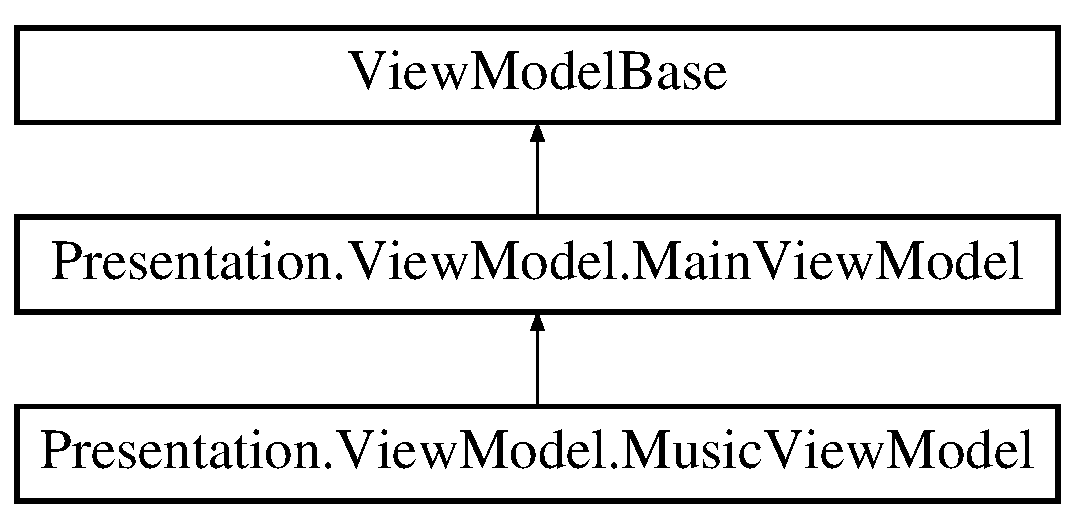
\includegraphics[height=3.000000cm]{class_presentation_1_1_view_model_1_1_music_view_model}
\end{center}
\end{figure}
\subsection*{Public Member Functions}
\begin{DoxyCompactItemize}
\item 
\mbox{\Hypertarget{class_presentation_1_1_view_model_1_1_music_view_model_a663da1779b44dad9622f6e87d335d1e5}\label{class_presentation_1_1_view_model_1_1_music_view_model_a663da1779b44dad9622f6e87d335d1e5}} 
{\bfseries Music\+View\+Model} (bool from\+Search)
\item 
\hyperlink{class_presentation_1_1_view_model_1_1_music_view_model_a2d9bfd47e3a2e98ac08cdfec449d69bf}{Music\+View\+Model} (Observable\+Collection$<$ \hyperlink{class_d_t_o_1_1_entity_1_1_track}{Track} $>$ tracks)
\begin{DoxyCompactList}\small\item\em When the view displays only tracks \end{DoxyCompactList}\item 
\hyperlink{class_presentation_1_1_view_model_1_1_music_view_model_a8230a35d252df28e6578be32bf6f8ba2}{Music\+View\+Model} (Observable\+Collection$<$ \hyperlink{class_d_t_o_1_1_entity_1_1_track}{Track} $>$ tracks, \hyperlink{class_d_t_o_1_1_entity_1_1_playlist}{Playlist} playlist)
\begin{DoxyCompactList}\small\item\em When the view is opened by the playlist viewmodel \end{DoxyCompactList}\item 
\hyperlink{class_presentation_1_1_view_model_1_1_music_view_model_a5856bb1decf95ae383427219e6598706}{Music\+View\+Model} (Observable\+Collection$<$ \hyperlink{class_d_t_o_1_1_entity_1_1_album}{Album} $>$ albums)
\begin{DoxyCompactList}\small\item\em When the view only display albums \end{DoxyCompactList}\item 
\hyperlink{class_presentation_1_1_view_model_1_1_music_view_model_a0b884bbf52c755226eac57a6b68a4e41}{Music\+View\+Model} (Observable\+Collection$<$ \hyperlink{class_d_t_o_1_1_entity_1_1_artist}{Artist} $>$ artists)
\begin{DoxyCompactList}\small\item\em When the view only display artists \end{DoxyCompactList}\item 
void \hyperlink{class_presentation_1_1_view_model_1_1_music_view_model_a5fc99c4453a0bb82e1b53091fa31b554}{Click\+Element} (object element)
\begin{DoxyCompactList}\small\item\em When an user click on an element, execute an action \end{DoxyCompactList}\item 
Observable\+Collection$<$ \hyperlink{class_d_t_o_1_1_context_menu}{Context\+Menu} $>$ \hyperlink{class_presentation_1_1_view_model_1_1_music_view_model_a70004ba66f44fcd3698d991bbc5c2856}{Create\+Playlist\+Menu} ()
\begin{DoxyCompactList}\small\item\em Create the context menu playlists \end{DoxyCompactList}\item 
void \hyperlink{class_presentation_1_1_view_model_1_1_music_view_model_af157154e1dc9f904c30b975626f26a85}{Removing\+From\+Playlist} (\hyperlink{class_d_t_o_1_1_entity_1_1_playlist}{Playlist} playlist)
\begin{DoxyCompactList}\small\item\em Remove a playlist \end{DoxyCompactList}\item 
void \hyperlink{class_presentation_1_1_view_model_1_1_music_view_model_a52a85cc7a7a537cdf36345fc83b5ab80}{Set\+Favorite} ()
\begin{DoxyCompactList}\small\item\em Set the list of all favorites musics \end{DoxyCompactList}\end{DoxyCompactItemize}
\subsection*{Properties}
\begin{DoxyCompactItemize}
\item 
\mbox{\Hypertarget{class_presentation_1_1_view_model_1_1_music_view_model_a343218f8efd58ceb0a2145926e871f4b}\label{class_presentation_1_1_view_model_1_1_music_view_model_a343218f8efd58ceb0a2145926e871f4b}} 
Observable\+Collection$<$ \hyperlink{class_d_t_o_1_1_entity_1_1_album}{Album} $>$ {\bfseries Albums}\hspace{0.3cm}{\ttfamily  \mbox{[}get, set\mbox{]}}
\item 
\mbox{\Hypertarget{class_presentation_1_1_view_model_1_1_music_view_model_ae5a6c636bbb67e6aecc47b2b7e3db3cf}\label{class_presentation_1_1_view_model_1_1_music_view_model_ae5a6c636bbb67e6aecc47b2b7e3db3cf}} 
Observable\+Collection$<$ \hyperlink{class_d_t_o_1_1_entity_1_1_artist}{Artist} $>$ {\bfseries Artists} = new Observable\+Collection$<$\hyperlink{class_d_t_o_1_1_entity_1_1_album}{Album}$>$()\hspace{0.3cm}{\ttfamily  \mbox{[}get, set\mbox{]}}
\item 
\mbox{\Hypertarget{class_presentation_1_1_view_model_1_1_music_view_model_a117bfb1393d36a49d4c1fdf636c04d00}\label{class_presentation_1_1_view_model_1_1_music_view_model_a117bfb1393d36a49d4c1fdf636c04d00}} 
Observable\+Collection$<$ \hyperlink{class_d_t_o_1_1_context_menu}{Context\+Menu} $>$ {\bfseries Context\+Menu} = new Observable\+Collection$<$\hyperlink{class_d_t_o_1_1_entity_1_1_artist}{Artist}$>$()\hspace{0.3cm}{\ttfamily  \mbox{[}get, set\mbox{]}}
\item 
\mbox{\Hypertarget{class_presentation_1_1_view_model_1_1_music_view_model_a2ec7de9cebab5ba2a33f7c13a7cd1176}\label{class_presentation_1_1_view_model_1_1_music_view_model_a2ec7de9cebab5ba2a33f7c13a7cd1176}} 
Observable\+Collection$<$ \hyperlink{class_d_t_o_1_1_entity_1_1_track}{Track} $>$ {\bfseries Favorites}\hspace{0.3cm}{\ttfamily  \mbox{[}get, set\mbox{]}}
\item 
\mbox{\Hypertarget{class_presentation_1_1_view_model_1_1_music_view_model_ad5cee341960517b1c950914de57a7b8f}\label{class_presentation_1_1_view_model_1_1_music_view_model_ad5cee341960517b1c950914de57a7b8f}} 
Observable\+Collection$<$ \hyperlink{class_d_t_o_1_1_entity_1_1_genre}{Genre} $>$ {\bfseries Genres} = new Observable\+Collection$<$\hyperlink{class_d_t_o_1_1_entity_1_1_track}{Track}$>$()\hspace{0.3cm}{\ttfamily  \mbox{[}get, set\mbox{]}}
\item 
\mbox{\Hypertarget{class_presentation_1_1_view_model_1_1_music_view_model_adb7851c333d8921cedee06bd4b23ea6e}\label{class_presentation_1_1_view_model_1_1_music_view_model_adb7851c333d8921cedee06bd4b23ea6e}} 
object {\bfseries Music\+Flyout\+View} = new Observable\+Collection$<$\hyperlink{class_d_t_o_1_1_entity_1_1_genre}{Genre}$>$()\hspace{0.3cm}{\ttfamily  \mbox{[}get, set\mbox{]}}
\item 
\mbox{\Hypertarget{class_presentation_1_1_view_model_1_1_music_view_model_ad38db33d3529525d2a8f992bee03f4a3}\label{class_presentation_1_1_view_model_1_1_music_view_model_ad38db33d3529525d2a8f992bee03f4a3}} 
Relay\+Command$<$ \hyperlink{class_d_t_o_1_1_entity_1_1_playlist}{Playlist} $>$ {\bfseries On\+Adding\+To\+Playlist}\hspace{0.3cm}{\ttfamily  \mbox{[}get, set\mbox{]}}
\item 
\mbox{\Hypertarget{class_presentation_1_1_view_model_1_1_music_view_model_ae59d20af276c2ad4a5d7257a34bf9c2a}\label{class_presentation_1_1_view_model_1_1_music_view_model_ae59d20af276c2ad4a5d7257a34bf9c2a}} 
Relay\+Command$<$ \hyperlink{class_d_t_o_1_1_entity_1_1_album}{Album} $>$ {\bfseries On\+Click\+Album\+Cover}\hspace{0.3cm}{\ttfamily  \mbox{[}get, set\mbox{]}}
\item 
\mbox{\Hypertarget{class_presentation_1_1_view_model_1_1_music_view_model_a4c4743a73d782bbe22383fa0aad68595}\label{class_presentation_1_1_view_model_1_1_music_view_model_a4c4743a73d782bbe22383fa0aad68595}} 
Relay\+Command {\bfseries On\+Click\+Element}\hspace{0.3cm}{\ttfamily  \mbox{[}get, set\mbox{]}}
\item 
\mbox{\Hypertarget{class_presentation_1_1_view_model_1_1_music_view_model_afa256cb737b2c2f309d7dbe511872725}\label{class_presentation_1_1_view_model_1_1_music_view_model_afa256cb737b2c2f309d7dbe511872725}} 
Relay\+Command {\bfseries On\+Creating\+Playlist}\hspace{0.3cm}{\ttfamily  \mbox{[}get, set\mbox{]}}
\item 
\mbox{\Hypertarget{class_presentation_1_1_view_model_1_1_music_view_model_af781706df7db4f8aae26e2f15c488afc}\label{class_presentation_1_1_view_model_1_1_music_view_model_af781706df7db4f8aae26e2f15c488afc}} 
Relay\+Command {\bfseries On\+Delete\+From\+Disk}\hspace{0.3cm}{\ttfamily  \mbox{[}get, set\mbox{]}}
\item 
\mbox{\Hypertarget{class_presentation_1_1_view_model_1_1_music_view_model_ac29d57f03ba9fcc3e5bb4f48dcb9ca6d}\label{class_presentation_1_1_view_model_1_1_music_view_model_ac29d57f03ba9fcc3e5bb4f48dcb9ca6d}} 
Relay\+Command {\bfseries On\+Delete\+From\+Library}\hspace{0.3cm}{\ttfamily  \mbox{[}get, set\mbox{]}}
\item 
\mbox{\Hypertarget{class_presentation_1_1_view_model_1_1_music_view_model_a24163ccbf96134920fb183118226ec6a}\label{class_presentation_1_1_view_model_1_1_music_view_model_a24163ccbf96134920fb183118226ec6a}} 
Relay\+Command$<$ \hyperlink{class_d_t_o_1_1_entity_1_1_playlist}{Playlist} $>$ {\bfseries On\+Removing\+From\+Playlist}\hspace{0.3cm}{\ttfamily  \mbox{[}get, set\mbox{]}}
\item 
\mbox{\Hypertarget{class_presentation_1_1_view_model_1_1_music_view_model_a6dc43da35d8e63b93dea75bbf3ba20fd}\label{class_presentation_1_1_view_model_1_1_music_view_model_a6dc43da35d8e63b93dea75bbf3ba20fd}} 
Relay\+Command {\bfseries On\+Right\+Click\+Track}\hspace{0.3cm}{\ttfamily  \mbox{[}get, set\mbox{]}}
\item 
\mbox{\Hypertarget{class_presentation_1_1_view_model_1_1_music_view_model_a43197789c9285bec96ec965e5b5fdd9a}\label{class_presentation_1_1_view_model_1_1_music_view_model_a43197789c9285bec96ec965e5b5fdd9a}} 
object {\bfseries Selected\+Item}\hspace{0.3cm}{\ttfamily  \mbox{[}get, set\mbox{]}}
\item 
\mbox{\Hypertarget{class_presentation_1_1_view_model_1_1_music_view_model_ae241135c15f2856a294078b5c7b6cd1b}\label{class_presentation_1_1_view_model_1_1_music_view_model_ae241135c15f2856a294078b5c7b6cd1b}} 
Observable\+Collection$<$ \hyperlink{class_d_t_o_1_1_entity_1_1_track}{Track} $>$ {\bfseries Tracks}\hspace{0.3cm}{\ttfamily  \mbox{[}get, set\mbox{]}}
\item 
\mbox{\Hypertarget{class_presentation_1_1_view_model_1_1_music_view_model_ada2313deba19ca5aba40e869bb22da41}\label{class_presentation_1_1_view_model_1_1_music_view_model_ada2313deba19ca5aba40e869bb22da41}} 
string {\bfseries Type} = new Observable\+Collection$<$\hyperlink{class_d_t_o_1_1_entity_1_1_track}{Track}$>$()\hspace{0.3cm}{\ttfamily  \mbox{[}get, set\mbox{]}}
\end{DoxyCompactItemize}


\subsection{Detailed Description}
This class contain the logic for the musicview 



\subsection{Constructor \& Destructor Documentation}
\mbox{\Hypertarget{class_presentation_1_1_view_model_1_1_music_view_model_a2d9bfd47e3a2e98ac08cdfec449d69bf}\label{class_presentation_1_1_view_model_1_1_music_view_model_a2d9bfd47e3a2e98ac08cdfec449d69bf}} 
\index{Presentation\+::\+View\+Model\+::\+Music\+View\+Model@{Presentation\+::\+View\+Model\+::\+Music\+View\+Model}!Music\+View\+Model@{Music\+View\+Model}}
\index{Music\+View\+Model@{Music\+View\+Model}!Presentation\+::\+View\+Model\+::\+Music\+View\+Model@{Presentation\+::\+View\+Model\+::\+Music\+View\+Model}}
\subsubsection{\texorpdfstring{Music\+View\+Model()}{MusicViewModel()}\hspace{0.1cm}{\footnotesize\ttfamily [1/4]}}
{\footnotesize\ttfamily Presentation.\+View\+Model.\+Music\+View\+Model.\+Music\+View\+Model (\begin{DoxyParamCaption}\item[{Observable\+Collection$<$ \hyperlink{class_d_t_o_1_1_entity_1_1_track}{Track} $>$}]{tracks }\end{DoxyParamCaption})}



When the view displays only tracks 


\begin{DoxyParams}{Parameters}
{\em tracks} & \\
\hline
\end{DoxyParams}
\mbox{\Hypertarget{class_presentation_1_1_view_model_1_1_music_view_model_a8230a35d252df28e6578be32bf6f8ba2}\label{class_presentation_1_1_view_model_1_1_music_view_model_a8230a35d252df28e6578be32bf6f8ba2}} 
\index{Presentation\+::\+View\+Model\+::\+Music\+View\+Model@{Presentation\+::\+View\+Model\+::\+Music\+View\+Model}!Music\+View\+Model@{Music\+View\+Model}}
\index{Music\+View\+Model@{Music\+View\+Model}!Presentation\+::\+View\+Model\+::\+Music\+View\+Model@{Presentation\+::\+View\+Model\+::\+Music\+View\+Model}}
\subsubsection{\texorpdfstring{Music\+View\+Model()}{MusicViewModel()}\hspace{0.1cm}{\footnotesize\ttfamily [2/4]}}
{\footnotesize\ttfamily Presentation.\+View\+Model.\+Music\+View\+Model.\+Music\+View\+Model (\begin{DoxyParamCaption}\item[{Observable\+Collection$<$ \hyperlink{class_d_t_o_1_1_entity_1_1_track}{Track} $>$}]{tracks,  }\item[{\hyperlink{class_d_t_o_1_1_entity_1_1_playlist}{Playlist}}]{playlist }\end{DoxyParamCaption})}



When the view is opened by the playlist viewmodel 


\begin{DoxyParams}{Parameters}
{\em tracks} & \\
\hline
{\em playlist} & \\
\hline
\end{DoxyParams}
\mbox{\Hypertarget{class_presentation_1_1_view_model_1_1_music_view_model_a5856bb1decf95ae383427219e6598706}\label{class_presentation_1_1_view_model_1_1_music_view_model_a5856bb1decf95ae383427219e6598706}} 
\index{Presentation\+::\+View\+Model\+::\+Music\+View\+Model@{Presentation\+::\+View\+Model\+::\+Music\+View\+Model}!Music\+View\+Model@{Music\+View\+Model}}
\index{Music\+View\+Model@{Music\+View\+Model}!Presentation\+::\+View\+Model\+::\+Music\+View\+Model@{Presentation\+::\+View\+Model\+::\+Music\+View\+Model}}
\subsubsection{\texorpdfstring{Music\+View\+Model()}{MusicViewModel()}\hspace{0.1cm}{\footnotesize\ttfamily [3/4]}}
{\footnotesize\ttfamily Presentation.\+View\+Model.\+Music\+View\+Model.\+Music\+View\+Model (\begin{DoxyParamCaption}\item[{Observable\+Collection$<$ \hyperlink{class_d_t_o_1_1_entity_1_1_album}{Album} $>$}]{albums }\end{DoxyParamCaption})}



When the view only display albums 


\begin{DoxyParams}{Parameters}
{\em albums} & \\
\hline
\end{DoxyParams}
\mbox{\Hypertarget{class_presentation_1_1_view_model_1_1_music_view_model_a0b884bbf52c755226eac57a6b68a4e41}\label{class_presentation_1_1_view_model_1_1_music_view_model_a0b884bbf52c755226eac57a6b68a4e41}} 
\index{Presentation\+::\+View\+Model\+::\+Music\+View\+Model@{Presentation\+::\+View\+Model\+::\+Music\+View\+Model}!Music\+View\+Model@{Music\+View\+Model}}
\index{Music\+View\+Model@{Music\+View\+Model}!Presentation\+::\+View\+Model\+::\+Music\+View\+Model@{Presentation\+::\+View\+Model\+::\+Music\+View\+Model}}
\subsubsection{\texorpdfstring{Music\+View\+Model()}{MusicViewModel()}\hspace{0.1cm}{\footnotesize\ttfamily [4/4]}}
{\footnotesize\ttfamily Presentation.\+View\+Model.\+Music\+View\+Model.\+Music\+View\+Model (\begin{DoxyParamCaption}\item[{Observable\+Collection$<$ \hyperlink{class_d_t_o_1_1_entity_1_1_artist}{Artist} $>$}]{artists }\end{DoxyParamCaption})}



When the view only display artists 


\begin{DoxyParams}{Parameters}
{\em albums} & \\
\hline
\end{DoxyParams}


\subsection{Member Function Documentation}
\mbox{\Hypertarget{class_presentation_1_1_view_model_1_1_music_view_model_a5fc99c4453a0bb82e1b53091fa31b554}\label{class_presentation_1_1_view_model_1_1_music_view_model_a5fc99c4453a0bb82e1b53091fa31b554}} 
\index{Presentation\+::\+View\+Model\+::\+Music\+View\+Model@{Presentation\+::\+View\+Model\+::\+Music\+View\+Model}!Click\+Element@{Click\+Element}}
\index{Click\+Element@{Click\+Element}!Presentation\+::\+View\+Model\+::\+Music\+View\+Model@{Presentation\+::\+View\+Model\+::\+Music\+View\+Model}}
\subsubsection{\texorpdfstring{Click\+Element()}{ClickElement()}}
{\footnotesize\ttfamily void Presentation.\+View\+Model.\+Music\+View\+Model.\+Click\+Element (\begin{DoxyParamCaption}\item[{object}]{element }\end{DoxyParamCaption})}



When an user click on an element, execute an action 


\begin{DoxyParams}{Parameters}
{\em element} & \\
\hline
\end{DoxyParams}
\mbox{\Hypertarget{class_presentation_1_1_view_model_1_1_music_view_model_a70004ba66f44fcd3698d991bbc5c2856}\label{class_presentation_1_1_view_model_1_1_music_view_model_a70004ba66f44fcd3698d991bbc5c2856}} 
\index{Presentation\+::\+View\+Model\+::\+Music\+View\+Model@{Presentation\+::\+View\+Model\+::\+Music\+View\+Model}!Create\+Playlist\+Menu@{Create\+Playlist\+Menu}}
\index{Create\+Playlist\+Menu@{Create\+Playlist\+Menu}!Presentation\+::\+View\+Model\+::\+Music\+View\+Model@{Presentation\+::\+View\+Model\+::\+Music\+View\+Model}}
\subsubsection{\texorpdfstring{Create\+Playlist\+Menu()}{CreatePlaylistMenu()}}
{\footnotesize\ttfamily Observable\+Collection$<$\hyperlink{class_d_t_o_1_1_context_menu}{Context\+Menu}$>$ Presentation.\+View\+Model.\+Music\+View\+Model.\+Create\+Playlist\+Menu (\begin{DoxyParamCaption}{ }\end{DoxyParamCaption})}



Create the context menu playlists 

\begin{DoxyReturn}{Returns}

\end{DoxyReturn}
\mbox{\Hypertarget{class_presentation_1_1_view_model_1_1_music_view_model_af157154e1dc9f904c30b975626f26a85}\label{class_presentation_1_1_view_model_1_1_music_view_model_af157154e1dc9f904c30b975626f26a85}} 
\index{Presentation\+::\+View\+Model\+::\+Music\+View\+Model@{Presentation\+::\+View\+Model\+::\+Music\+View\+Model}!Removing\+From\+Playlist@{Removing\+From\+Playlist}}
\index{Removing\+From\+Playlist@{Removing\+From\+Playlist}!Presentation\+::\+View\+Model\+::\+Music\+View\+Model@{Presentation\+::\+View\+Model\+::\+Music\+View\+Model}}
\subsubsection{\texorpdfstring{Removing\+From\+Playlist()}{RemovingFromPlaylist()}}
{\footnotesize\ttfamily void Presentation.\+View\+Model.\+Music\+View\+Model.\+Removing\+From\+Playlist (\begin{DoxyParamCaption}\item[{\hyperlink{class_d_t_o_1_1_entity_1_1_playlist}{Playlist}}]{playlist }\end{DoxyParamCaption})}



Remove a playlist 


\begin{DoxyParams}{Parameters}
{\em playlist} & \\
\hline
\end{DoxyParams}
\mbox{\Hypertarget{class_presentation_1_1_view_model_1_1_music_view_model_a52a85cc7a7a537cdf36345fc83b5ab80}\label{class_presentation_1_1_view_model_1_1_music_view_model_a52a85cc7a7a537cdf36345fc83b5ab80}} 
\index{Presentation\+::\+View\+Model\+::\+Music\+View\+Model@{Presentation\+::\+View\+Model\+::\+Music\+View\+Model}!Set\+Favorite@{Set\+Favorite}}
\index{Set\+Favorite@{Set\+Favorite}!Presentation\+::\+View\+Model\+::\+Music\+View\+Model@{Presentation\+::\+View\+Model\+::\+Music\+View\+Model}}
\subsubsection{\texorpdfstring{Set\+Favorite()}{SetFavorite()}}
{\footnotesize\ttfamily void Presentation.\+View\+Model.\+Music\+View\+Model.\+Set\+Favorite (\begin{DoxyParamCaption}{ }\end{DoxyParamCaption})}



Set the list of all favorites musics 



The documentation for this class was generated from the following file\+:\begin{DoxyCompactItemize}
\item 
C\+:/\+W\+O\+R\+K\+S\+P\+A\+C\+E/\+T\+P\+I-\/end/\+Gestion\+Audio/\+Gestion\+Audio/\+View\+Model/Music\+View\+Model.\+cs\end{DoxyCompactItemize}

\hypertarget{class_presentation_1_1_view_model_1_1_player_view_model}{}\section{Presentation.\+View\+Model.\+Player\+View\+Model Class Reference}
\label{class_presentation_1_1_view_model_1_1_player_view_model}\index{Presentation.\+View\+Model.\+Player\+View\+Model@{Presentation.\+View\+Model.\+Player\+View\+Model}}


This class contain the logic for the small and big player  


Inheritance diagram for Presentation.\+View\+Model.\+Player\+View\+Model\+:\begin{figure}[H]
\begin{center}
\leavevmode
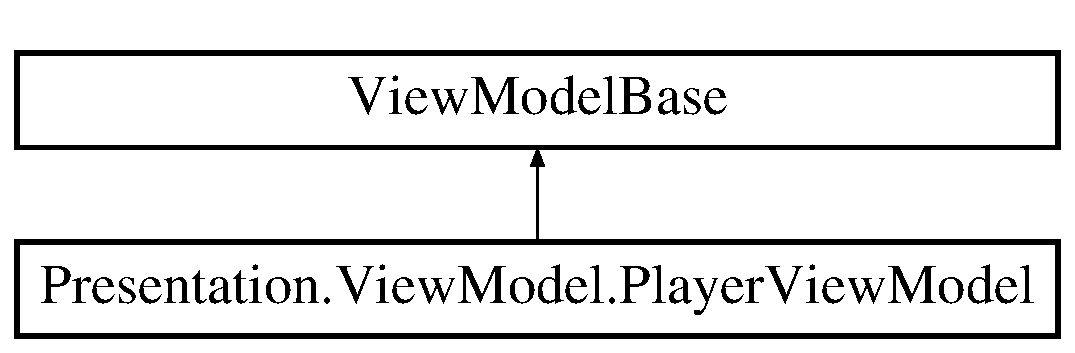
\includegraphics[height=2.000000cm]{class_presentation_1_1_view_model_1_1_player_view_model}
\end{center}
\end{figure}
\subsection*{Public Member Functions}
\begin{DoxyCompactItemize}
\item 
void \hyperlink{class_presentation_1_1_view_model_1_1_player_view_model_ae27f5e428604e168e00216a5775e4f20}{Change\+Time\+To\+Slider} (int milisecond, int total)
\begin{DoxyCompactList}\small\item\em Change the time of the slider \end{DoxyCompactList}\item 
void \hyperlink{class_presentation_1_1_view_model_1_1_player_view_model_af4b8393d4c9fa02c0f77ae12b43ddf26}{Click\+Favorite} ()
\begin{DoxyCompactList}\small\item\em When the user click on the favorite/unfavorite logo \end{DoxyCompactList}\item 
\mbox{\Hypertarget{class_presentation_1_1_view_model_1_1_player_view_model_a4abef53bb3e901572373320a0f9bb573}\label{class_presentation_1_1_view_model_1_1_player_view_model_a4abef53bb3e901572373320a0f9bb573}} 
void {\bfseries Click\+Forward} ()
\item 
void \hyperlink{class_presentation_1_1_view_model_1_1_player_view_model_aa465600947e868db782dcefc4c583397}{Click\+Loop\+Reading\+List} ()
\begin{DoxyCompactList}\small\item\em change the lecture type (straight -\/$>$ continous) \end{DoxyCompactList}\item 
void \hyperlink{class_presentation_1_1_view_model_1_1_player_view_model_ac179d33971d45dca1de5807ad70541f3}{Click\+Picture} ()
\begin{DoxyCompactList}\small\item\em When the user click on the picture, open the running flyout \end{DoxyCompactList}\item 
void \hyperlink{class_presentation_1_1_view_model_1_1_player_view_model_aab7033d6e657e0d4655c07c2e9a64527}{Click\+Play} ()
\begin{DoxyCompactList}\small\item\em Play the music \end{DoxyCompactList}\item 
void \hyperlink{class_presentation_1_1_view_model_1_1_player_view_model_ac07fc3f368638796014fac0079173b7f}{Click\+Random} ()
\begin{DoxyCompactList}\small\item\em When the user click on the random button \end{DoxyCompactList}\item 
void \hyperlink{class_presentation_1_1_view_model_1_1_player_view_model_a522861826c27d85dc5df4b9f629c4f14}{Click\+Reading\+List} ()
\begin{DoxyCompactList}\small\item\em Show the reading list \end{DoxyCompactList}\item 
void \hyperlink{class_presentation_1_1_view_model_1_1_player_view_model_a498f0356e1ea32517ac3f63d49de25b7}{Click\+Rewind} ()
\begin{DoxyCompactList}\small\item\em Go to previous music \end{DoxyCompactList}\item 
void \hyperlink{class_presentation_1_1_view_model_1_1_player_view_model_a0bb79b71a852316176dd3e8ff860a62f}{Init\+Player} (\hyperlink{class_d_t_o_1_1_audio}{Audio} audio)
\begin{DoxyCompactList}\small\item\em Set up a track \end{DoxyCompactList}\item 
void \hyperlink{class_presentation_1_1_view_model_1_1_player_view_model_a07da028812b546a5f7083cd1b460ddc7}{Mousedown\+Forward} ()
\begin{DoxyCompactList}\small\item\em When the user hold down the forward button \end{DoxyCompactList}\item 
void \hyperlink{class_presentation_1_1_view_model_1_1_player_view_model_a9239c10b2baf32dbec43fb6a15e902a8}{Mousedown\+Rewind} ()
\begin{DoxyCompactList}\small\item\em When the user hold down the rewind button \end{DoxyCompactList}\end{DoxyCompactItemize}
\subsection*{Properties}
\begin{DoxyCompactItemize}
\item 
\mbox{\Hypertarget{class_presentation_1_1_view_model_1_1_player_view_model_a82f91763549ae2ae217d9c7b763c8a02}\label{class_presentation_1_1_view_model_1_1_player_view_model_a82f91763549ae2ae217d9c7b763c8a02}} 
Time\+Span {\bfseries Actual\+Time}\hspace{0.3cm}{\ttfamily  \mbox{[}get, set\mbox{]}}
\item 
\mbox{\Hypertarget{class_presentation_1_1_view_model_1_1_player_view_model_a1efb50e45444346dfee980431b7c745a}\label{class_presentation_1_1_view_model_1_1_player_view_model_a1efb50e45444346dfee980431b7c745a}} 
\hyperlink{class_d_t_o_1_1_audio}{Audio} {\bfseries Audio}\hspace{0.3cm}{\ttfamily  \mbox{[}get, set\mbox{]}}
\item 
\mbox{\Hypertarget{class_presentation_1_1_view_model_1_1_player_view_model_ac384a0d499e32102f6b732364245828b}\label{class_presentation_1_1_view_model_1_1_player_view_model_ac384a0d499e32102f6b732364245828b}} 
int {\bfseries Is\+Looping}\hspace{0.3cm}{\ttfamily  \mbox{[}get, set\mbox{]}}
\item 
\mbox{\Hypertarget{class_presentation_1_1_view_model_1_1_player_view_model_a501f2f29b5cc77999918548d8cdbd862}\label{class_presentation_1_1_view_model_1_1_player_view_model_a501f2f29b5cc77999918548d8cdbd862}} 
Visibility {\bfseries Is\+Radio}\hspace{0.3cm}{\ttfamily  \mbox{[}get, set\mbox{]}}
\item 
\mbox{\Hypertarget{class_presentation_1_1_view_model_1_1_player_view_model_a81e89c646f87f798db0f346d24a537c8}\label{class_presentation_1_1_view_model_1_1_player_view_model_a81e89c646f87f798db0f346d24a537c8}} 
bool {\bfseries Is\+Random}\hspace{0.3cm}{\ttfamily  \mbox{[}get, set\mbox{]}}
\item 
\mbox{\Hypertarget{class_presentation_1_1_view_model_1_1_player_view_model_aa1c1c8c30b1fddf299dc6291e5f13976}\label{class_presentation_1_1_view_model_1_1_player_view_model_aa1c1c8c30b1fddf299dc6291e5f13976}} 
Relay\+Command {\bfseries On\+Click\+Favorite}\hspace{0.3cm}{\ttfamily  \mbox{[}get, set\mbox{]}}
\item 
\mbox{\Hypertarget{class_presentation_1_1_view_model_1_1_player_view_model_ad040c8e75972f75933e8e727b4df220f}\label{class_presentation_1_1_view_model_1_1_player_view_model_ad040c8e75972f75933e8e727b4df220f}} 
Relay\+Command {\bfseries On\+Click\+Loop\+Reading\+List}\hspace{0.3cm}{\ttfamily  \mbox{[}get, set\mbox{]}}
\item 
\mbox{\Hypertarget{class_presentation_1_1_view_model_1_1_player_view_model_a087b009ae16712410ed741d2bf1aa48b}\label{class_presentation_1_1_view_model_1_1_player_view_model_a087b009ae16712410ed741d2bf1aa48b}} 
Relay\+Command {\bfseries On\+Click\+Picture}\hspace{0.3cm}{\ttfamily  \mbox{[}get, set\mbox{]}}
\item 
\mbox{\Hypertarget{class_presentation_1_1_view_model_1_1_player_view_model_a1cb8bbf887846e514842d50e96de8dc4}\label{class_presentation_1_1_view_model_1_1_player_view_model_a1cb8bbf887846e514842d50e96de8dc4}} 
Relay\+Command {\bfseries On\+Click\+Play}\hspace{0.3cm}{\ttfamily  \mbox{[}get, set\mbox{]}}
\item 
\mbox{\Hypertarget{class_presentation_1_1_view_model_1_1_player_view_model_a4176ddc01e2c374b7b568037b6a3b770}\label{class_presentation_1_1_view_model_1_1_player_view_model_a4176ddc01e2c374b7b568037b6a3b770}} 
Relay\+Command {\bfseries On\+Click\+Random}\hspace{0.3cm}{\ttfamily  \mbox{[}get, set\mbox{]}}
\item 
\mbox{\Hypertarget{class_presentation_1_1_view_model_1_1_player_view_model_ac1e5c4cfbbc3549757114ce403f7db6f}\label{class_presentation_1_1_view_model_1_1_player_view_model_ac1e5c4cfbbc3549757114ce403f7db6f}} 
Relay\+Command {\bfseries On\+Click\+Reading\+List}\hspace{0.3cm}{\ttfamily  \mbox{[}get, set\mbox{]}}
\item 
\mbox{\Hypertarget{class_presentation_1_1_view_model_1_1_player_view_model_a1cd7fbf86e75b53e081a1a170a5622e2}\label{class_presentation_1_1_view_model_1_1_player_view_model_a1cd7fbf86e75b53e081a1a170a5622e2}} 
Relay\+Command {\bfseries On\+Mousedown\+Forward}\hspace{0.3cm}{\ttfamily  \mbox{[}get, set\mbox{]}}
\item 
\mbox{\Hypertarget{class_presentation_1_1_view_model_1_1_player_view_model_a0e65c91b75bedb24a71656f5347fcc47}\label{class_presentation_1_1_view_model_1_1_player_view_model_a0e65c91b75bedb24a71656f5347fcc47}} 
Relay\+Command {\bfseries On\+Mousedown\+Rewind}\hspace{0.3cm}{\ttfamily  \mbox{[}get, set\mbox{]}}
\item 
\mbox{\Hypertarget{class_presentation_1_1_view_model_1_1_player_view_model_a47d8955accfeef86a15e2f9df099a475}\label{class_presentation_1_1_view_model_1_1_player_view_model_a47d8955accfeef86a15e2f9df099a475}} 
bool {\bfseries Playler\+Status}\hspace{0.3cm}{\ttfamily  \mbox{[}get, set\mbox{]}}
\item 
\mbox{\Hypertarget{class_presentation_1_1_view_model_1_1_player_view_model_a85051176aa367598c5f33c1a10fa787e}\label{class_presentation_1_1_view_model_1_1_player_view_model_a85051176aa367598c5f33c1a10fa787e}} 
double {\bfseries Slider\+Value}\hspace{0.3cm}{\ttfamily  \mbox{[}get, set\mbox{]}}
\item 
\mbox{\Hypertarget{class_presentation_1_1_view_model_1_1_player_view_model_a4f12efdf37816186501830f40bf0bb09}\label{class_presentation_1_1_view_model_1_1_player_view_model_a4f12efdf37816186501830f40bf0bb09}} 
float {\bfseries Volume\+Value}\hspace{0.3cm}{\ttfamily  \mbox{[}get, set\mbox{]}}
\end{DoxyCompactItemize}


\subsection{Detailed Description}
This class contain the logic for the small and big player 



\subsection{Member Function Documentation}
\mbox{\Hypertarget{class_presentation_1_1_view_model_1_1_player_view_model_ae27f5e428604e168e00216a5775e4f20}\label{class_presentation_1_1_view_model_1_1_player_view_model_ae27f5e428604e168e00216a5775e4f20}} 
\index{Presentation\+::\+View\+Model\+::\+Player\+View\+Model@{Presentation\+::\+View\+Model\+::\+Player\+View\+Model}!Change\+Time\+To\+Slider@{Change\+Time\+To\+Slider}}
\index{Change\+Time\+To\+Slider@{Change\+Time\+To\+Slider}!Presentation\+::\+View\+Model\+::\+Player\+View\+Model@{Presentation\+::\+View\+Model\+::\+Player\+View\+Model}}
\subsubsection{\texorpdfstring{Change\+Time\+To\+Slider()}{ChangeTimeToSlider()}}
{\footnotesize\ttfamily void Presentation.\+View\+Model.\+Player\+View\+Model.\+Change\+Time\+To\+Slider (\begin{DoxyParamCaption}\item[{int}]{milisecond,  }\item[{int}]{total }\end{DoxyParamCaption})}



Change the time of the slider 


\begin{DoxyParams}{Parameters}
{\em milisecond} & \\
\hline
{\em total} & \\
\hline
\end{DoxyParams}
\mbox{\Hypertarget{class_presentation_1_1_view_model_1_1_player_view_model_af4b8393d4c9fa02c0f77ae12b43ddf26}\label{class_presentation_1_1_view_model_1_1_player_view_model_af4b8393d4c9fa02c0f77ae12b43ddf26}} 
\index{Presentation\+::\+View\+Model\+::\+Player\+View\+Model@{Presentation\+::\+View\+Model\+::\+Player\+View\+Model}!Click\+Favorite@{Click\+Favorite}}
\index{Click\+Favorite@{Click\+Favorite}!Presentation\+::\+View\+Model\+::\+Player\+View\+Model@{Presentation\+::\+View\+Model\+::\+Player\+View\+Model}}
\subsubsection{\texorpdfstring{Click\+Favorite()}{ClickFavorite()}}
{\footnotesize\ttfamily void Presentation.\+View\+Model.\+Player\+View\+Model.\+Click\+Favorite (\begin{DoxyParamCaption}{ }\end{DoxyParamCaption})}



When the user click on the favorite/unfavorite logo 

\mbox{\Hypertarget{class_presentation_1_1_view_model_1_1_player_view_model_aa465600947e868db782dcefc4c583397}\label{class_presentation_1_1_view_model_1_1_player_view_model_aa465600947e868db782dcefc4c583397}} 
\index{Presentation\+::\+View\+Model\+::\+Player\+View\+Model@{Presentation\+::\+View\+Model\+::\+Player\+View\+Model}!Click\+Loop\+Reading\+List@{Click\+Loop\+Reading\+List}}
\index{Click\+Loop\+Reading\+List@{Click\+Loop\+Reading\+List}!Presentation\+::\+View\+Model\+::\+Player\+View\+Model@{Presentation\+::\+View\+Model\+::\+Player\+View\+Model}}
\subsubsection{\texorpdfstring{Click\+Loop\+Reading\+List()}{ClickLoopReadingList()}}
{\footnotesize\ttfamily void Presentation.\+View\+Model.\+Player\+View\+Model.\+Click\+Loop\+Reading\+List (\begin{DoxyParamCaption}{ }\end{DoxyParamCaption})}



change the lecture type (straight -\/$>$ continous) 

\mbox{\Hypertarget{class_presentation_1_1_view_model_1_1_player_view_model_ac179d33971d45dca1de5807ad70541f3}\label{class_presentation_1_1_view_model_1_1_player_view_model_ac179d33971d45dca1de5807ad70541f3}} 
\index{Presentation\+::\+View\+Model\+::\+Player\+View\+Model@{Presentation\+::\+View\+Model\+::\+Player\+View\+Model}!Click\+Picture@{Click\+Picture}}
\index{Click\+Picture@{Click\+Picture}!Presentation\+::\+View\+Model\+::\+Player\+View\+Model@{Presentation\+::\+View\+Model\+::\+Player\+View\+Model}}
\subsubsection{\texorpdfstring{Click\+Picture()}{ClickPicture()}}
{\footnotesize\ttfamily void Presentation.\+View\+Model.\+Player\+View\+Model.\+Click\+Picture (\begin{DoxyParamCaption}{ }\end{DoxyParamCaption})}



When the user click on the picture, open the running flyout 

\mbox{\Hypertarget{class_presentation_1_1_view_model_1_1_player_view_model_aab7033d6e657e0d4655c07c2e9a64527}\label{class_presentation_1_1_view_model_1_1_player_view_model_aab7033d6e657e0d4655c07c2e9a64527}} 
\index{Presentation\+::\+View\+Model\+::\+Player\+View\+Model@{Presentation\+::\+View\+Model\+::\+Player\+View\+Model}!Click\+Play@{Click\+Play}}
\index{Click\+Play@{Click\+Play}!Presentation\+::\+View\+Model\+::\+Player\+View\+Model@{Presentation\+::\+View\+Model\+::\+Player\+View\+Model}}
\subsubsection{\texorpdfstring{Click\+Play()}{ClickPlay()}}
{\footnotesize\ttfamily void Presentation.\+View\+Model.\+Player\+View\+Model.\+Click\+Play (\begin{DoxyParamCaption}{ }\end{DoxyParamCaption})}



Play the music 

\mbox{\Hypertarget{class_presentation_1_1_view_model_1_1_player_view_model_ac07fc3f368638796014fac0079173b7f}\label{class_presentation_1_1_view_model_1_1_player_view_model_ac07fc3f368638796014fac0079173b7f}} 
\index{Presentation\+::\+View\+Model\+::\+Player\+View\+Model@{Presentation\+::\+View\+Model\+::\+Player\+View\+Model}!Click\+Random@{Click\+Random}}
\index{Click\+Random@{Click\+Random}!Presentation\+::\+View\+Model\+::\+Player\+View\+Model@{Presentation\+::\+View\+Model\+::\+Player\+View\+Model}}
\subsubsection{\texorpdfstring{Click\+Random()}{ClickRandom()}}
{\footnotesize\ttfamily void Presentation.\+View\+Model.\+Player\+View\+Model.\+Click\+Random (\begin{DoxyParamCaption}{ }\end{DoxyParamCaption})}



When the user click on the random button 

\mbox{\Hypertarget{class_presentation_1_1_view_model_1_1_player_view_model_a522861826c27d85dc5df4b9f629c4f14}\label{class_presentation_1_1_view_model_1_1_player_view_model_a522861826c27d85dc5df4b9f629c4f14}} 
\index{Presentation\+::\+View\+Model\+::\+Player\+View\+Model@{Presentation\+::\+View\+Model\+::\+Player\+View\+Model}!Click\+Reading\+List@{Click\+Reading\+List}}
\index{Click\+Reading\+List@{Click\+Reading\+List}!Presentation\+::\+View\+Model\+::\+Player\+View\+Model@{Presentation\+::\+View\+Model\+::\+Player\+View\+Model}}
\subsubsection{\texorpdfstring{Click\+Reading\+List()}{ClickReadingList()}}
{\footnotesize\ttfamily void Presentation.\+View\+Model.\+Player\+View\+Model.\+Click\+Reading\+List (\begin{DoxyParamCaption}{ }\end{DoxyParamCaption})}



Show the reading list 

\mbox{\Hypertarget{class_presentation_1_1_view_model_1_1_player_view_model_a498f0356e1ea32517ac3f63d49de25b7}\label{class_presentation_1_1_view_model_1_1_player_view_model_a498f0356e1ea32517ac3f63d49de25b7}} 
\index{Presentation\+::\+View\+Model\+::\+Player\+View\+Model@{Presentation\+::\+View\+Model\+::\+Player\+View\+Model}!Click\+Rewind@{Click\+Rewind}}
\index{Click\+Rewind@{Click\+Rewind}!Presentation\+::\+View\+Model\+::\+Player\+View\+Model@{Presentation\+::\+View\+Model\+::\+Player\+View\+Model}}
\subsubsection{\texorpdfstring{Click\+Rewind()}{ClickRewind()}}
{\footnotesize\ttfamily void Presentation.\+View\+Model.\+Player\+View\+Model.\+Click\+Rewind (\begin{DoxyParamCaption}{ }\end{DoxyParamCaption})}



Go to previous music 

\mbox{\Hypertarget{class_presentation_1_1_view_model_1_1_player_view_model_a0bb79b71a852316176dd3e8ff860a62f}\label{class_presentation_1_1_view_model_1_1_player_view_model_a0bb79b71a852316176dd3e8ff860a62f}} 
\index{Presentation\+::\+View\+Model\+::\+Player\+View\+Model@{Presentation\+::\+View\+Model\+::\+Player\+View\+Model}!Init\+Player@{Init\+Player}}
\index{Init\+Player@{Init\+Player}!Presentation\+::\+View\+Model\+::\+Player\+View\+Model@{Presentation\+::\+View\+Model\+::\+Player\+View\+Model}}
\subsubsection{\texorpdfstring{Init\+Player()}{InitPlayer()}}
{\footnotesize\ttfamily void Presentation.\+View\+Model.\+Player\+View\+Model.\+Init\+Player (\begin{DoxyParamCaption}\item[{\hyperlink{class_d_t_o_1_1_audio}{Audio}}]{audio }\end{DoxyParamCaption})}



Set up a track 


\begin{DoxyParams}{Parameters}
{\em audio} & \\
\hline
\end{DoxyParams}
\mbox{\Hypertarget{class_presentation_1_1_view_model_1_1_player_view_model_a07da028812b546a5f7083cd1b460ddc7}\label{class_presentation_1_1_view_model_1_1_player_view_model_a07da028812b546a5f7083cd1b460ddc7}} 
\index{Presentation\+::\+View\+Model\+::\+Player\+View\+Model@{Presentation\+::\+View\+Model\+::\+Player\+View\+Model}!Mousedown\+Forward@{Mousedown\+Forward}}
\index{Mousedown\+Forward@{Mousedown\+Forward}!Presentation\+::\+View\+Model\+::\+Player\+View\+Model@{Presentation\+::\+View\+Model\+::\+Player\+View\+Model}}
\subsubsection{\texorpdfstring{Mousedown\+Forward()}{MousedownForward()}}
{\footnotesize\ttfamily void Presentation.\+View\+Model.\+Player\+View\+Model.\+Mousedown\+Forward (\begin{DoxyParamCaption}{ }\end{DoxyParamCaption})}



When the user hold down the forward button 

\mbox{\Hypertarget{class_presentation_1_1_view_model_1_1_player_view_model_a9239c10b2baf32dbec43fb6a15e902a8}\label{class_presentation_1_1_view_model_1_1_player_view_model_a9239c10b2baf32dbec43fb6a15e902a8}} 
\index{Presentation\+::\+View\+Model\+::\+Player\+View\+Model@{Presentation\+::\+View\+Model\+::\+Player\+View\+Model}!Mousedown\+Rewind@{Mousedown\+Rewind}}
\index{Mousedown\+Rewind@{Mousedown\+Rewind}!Presentation\+::\+View\+Model\+::\+Player\+View\+Model@{Presentation\+::\+View\+Model\+::\+Player\+View\+Model}}
\subsubsection{\texorpdfstring{Mousedown\+Rewind()}{MousedownRewind()}}
{\footnotesize\ttfamily void Presentation.\+View\+Model.\+Player\+View\+Model.\+Mousedown\+Rewind (\begin{DoxyParamCaption}{ }\end{DoxyParamCaption})}



When the user hold down the rewind button 



The documentation for this class was generated from the following file\+:\begin{DoxyCompactItemize}
\item 
C\+:/\+W\+O\+R\+K\+S\+P\+A\+C\+E/\+T\+P\+I-\/end/\+Gestion\+Audio/\+Gestion\+Audio/\+View\+Model/Player\+View\+Model.\+cs\end{DoxyCompactItemize}

\hypertarget{class_d_t_o_1_1_entity_1_1_playlist}{}\section{D\+T\+O.\+Entity.\+Playlist Class Reference}
\label{class_d_t_o_1_1_entity_1_1_playlist}\index{D\+T\+O.\+Entity.\+Playlist@{D\+T\+O.\+Entity.\+Playlist}}


The database \hyperlink{class_d_t_o_1_1_entity_1_1_playlist}{Playlist} entity  


Inheritance diagram for D\+T\+O.\+Entity.\+Playlist\+:\begin{figure}[H]
\begin{center}
\leavevmode
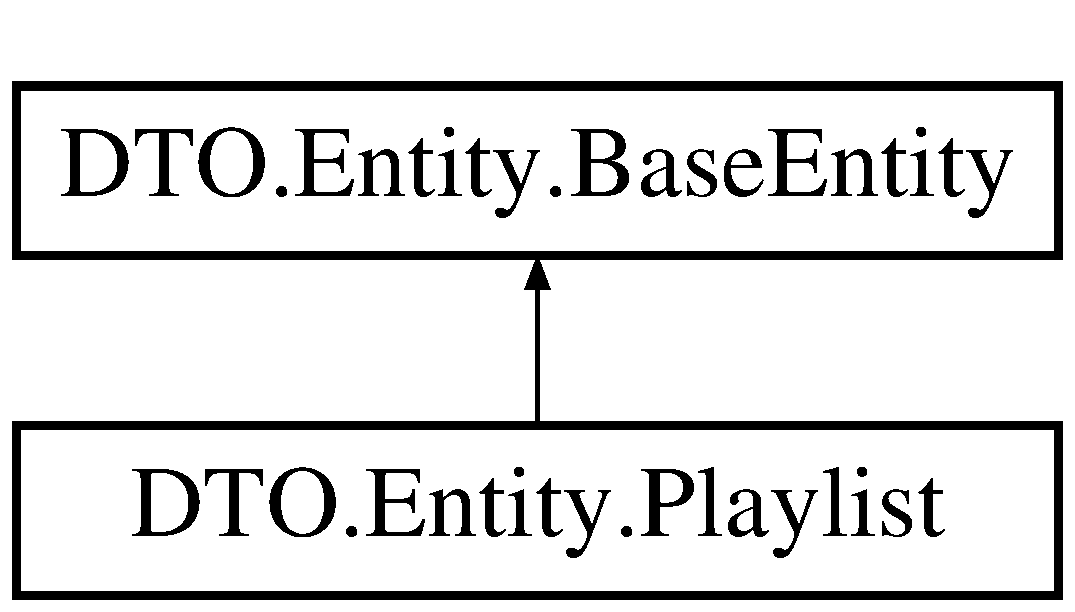
\includegraphics[height=2.000000cm]{class_d_t_o_1_1_entity_1_1_playlist}
\end{center}
\end{figure}
\subsection*{Properties}
\begin{DoxyCompactItemize}
\item 
\mbox{\Hypertarget{class_d_t_o_1_1_entity_1_1_playlist_a9e384c0b935acf1f89e227fefda92e6c}\label{class_d_t_o_1_1_entity_1_1_playlist_a9e384c0b935acf1f89e227fefda92e6c}} 
string {\bfseries Name}\hspace{0.3cm}{\ttfamily  \mbox{[}get, set\mbox{]}}
\item 
\mbox{\Hypertarget{class_d_t_o_1_1_entity_1_1_playlist_a54e6e840c74fca0128bdb0b7cd41b26b}\label{class_d_t_o_1_1_entity_1_1_playlist_a54e6e840c74fca0128bdb0b7cd41b26b}} 
virtual List$<$ \hyperlink{class_d_t_o_1_1_entity_1_1_track}{Track} $>$ {\bfseries Tracks}\hspace{0.3cm}{\ttfamily  \mbox{[}get, set\mbox{]}}
\end{DoxyCompactItemize}


\subsection{Detailed Description}
The database \hyperlink{class_d_t_o_1_1_entity_1_1_playlist}{Playlist} entity 



The documentation for this class was generated from the following file\+:\begin{DoxyCompactItemize}
\item 
C\+:/\+W\+O\+R\+K\+S\+P\+A\+C\+E/\+T\+P\+I-\/end/\+Gestion\+Audio/\+D\+T\+O/\+Entity/Playlist.\+cs\end{DoxyCompactItemize}

\hypertarget{class_presentation_1_1_view_1_1_list_1_1_playlist_list_view}{}\section{Presentation.\+View.\+List.\+Playlist\+List\+View Class Reference}
\label{class_presentation_1_1_view_1_1_list_1_1_playlist_list_view}\index{Presentation.\+View.\+List.\+Playlist\+List\+View@{Presentation.\+View.\+List.\+Playlist\+List\+View}}


\hyperlink{class_presentation_1_1_view_1_1_list_1_1_playlist_list_view}{Playlist\+List\+View}  


Inheritance diagram for Presentation.\+View.\+List.\+Playlist\+List\+View\+:\begin{figure}[H]
\begin{center}
\leavevmode
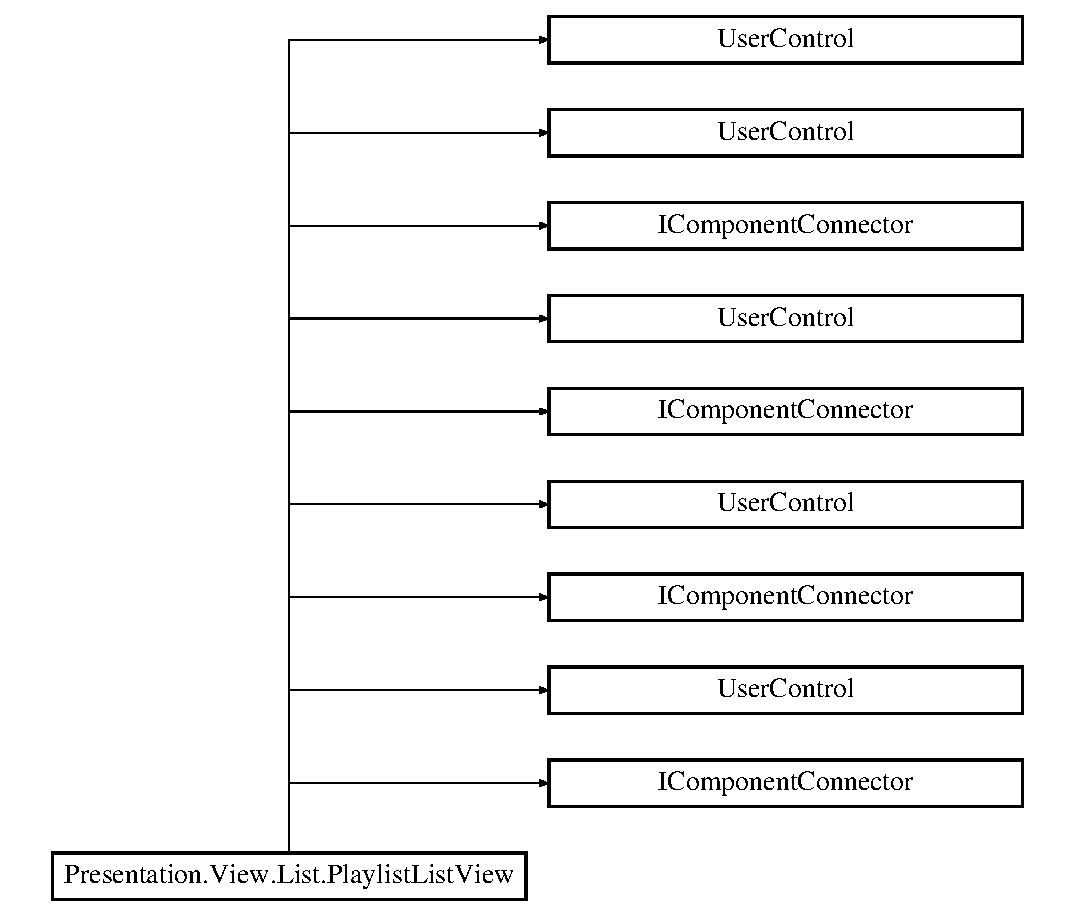
\includegraphics[height=10.000000cm]{class_presentation_1_1_view_1_1_list_1_1_playlist_list_view}
\end{center}
\end{figure}
\subsection*{Public Member Functions}
\begin{DoxyCompactItemize}
\item 
void \hyperlink{class_presentation_1_1_view_1_1_list_1_1_playlist_list_view_aa9bf1ecd779db592df3c013a92d6e218}{Initialize\+Component} ()
\begin{DoxyCompactList}\small\item\em Initialize\+Component \end{DoxyCompactList}\item 
void \hyperlink{class_presentation_1_1_view_1_1_list_1_1_playlist_list_view_aa9bf1ecd779db592df3c013a92d6e218}{Initialize\+Component} ()
\begin{DoxyCompactList}\small\item\em Initialize\+Component \end{DoxyCompactList}\item 
void \hyperlink{class_presentation_1_1_view_1_1_list_1_1_playlist_list_view_aa9bf1ecd779db592df3c013a92d6e218}{Initialize\+Component} ()
\begin{DoxyCompactList}\small\item\em Initialize\+Component \end{DoxyCompactList}\item 
void \hyperlink{class_presentation_1_1_view_1_1_list_1_1_playlist_list_view_aa9bf1ecd779db592df3c013a92d6e218}{Initialize\+Component} ()
\begin{DoxyCompactList}\small\item\em Initialize\+Component \end{DoxyCompactList}\end{DoxyCompactItemize}


\subsection{Detailed Description}
\hyperlink{class_presentation_1_1_view_1_1_list_1_1_playlist_list_view}{Playlist\+List\+View} 

Interaction logic for Music\+Home.\+xaml 

\subsection{Member Function Documentation}
\mbox{\Hypertarget{class_presentation_1_1_view_1_1_list_1_1_playlist_list_view_aa9bf1ecd779db592df3c013a92d6e218}\label{class_presentation_1_1_view_1_1_list_1_1_playlist_list_view_aa9bf1ecd779db592df3c013a92d6e218}} 
\index{Presentation\+::\+View\+::\+List\+::\+Playlist\+List\+View@{Presentation\+::\+View\+::\+List\+::\+Playlist\+List\+View}!Initialize\+Component@{Initialize\+Component}}
\index{Initialize\+Component@{Initialize\+Component}!Presentation\+::\+View\+::\+List\+::\+Playlist\+List\+View@{Presentation\+::\+View\+::\+List\+::\+Playlist\+List\+View}}
\subsubsection{\texorpdfstring{Initialize\+Component()}{InitializeComponent()}\hspace{0.1cm}{\footnotesize\ttfamily [1/4]}}
{\footnotesize\ttfamily void Presentation.\+View.\+List.\+Playlist\+List\+View.\+Initialize\+Component (\begin{DoxyParamCaption}{ }\end{DoxyParamCaption})}



Initialize\+Component 

\mbox{\Hypertarget{class_presentation_1_1_view_1_1_list_1_1_playlist_list_view_aa9bf1ecd779db592df3c013a92d6e218}\label{class_presentation_1_1_view_1_1_list_1_1_playlist_list_view_aa9bf1ecd779db592df3c013a92d6e218}} 
\index{Presentation\+::\+View\+::\+List\+::\+Playlist\+List\+View@{Presentation\+::\+View\+::\+List\+::\+Playlist\+List\+View}!Initialize\+Component@{Initialize\+Component}}
\index{Initialize\+Component@{Initialize\+Component}!Presentation\+::\+View\+::\+List\+::\+Playlist\+List\+View@{Presentation\+::\+View\+::\+List\+::\+Playlist\+List\+View}}
\subsubsection{\texorpdfstring{Initialize\+Component()}{InitializeComponent()}\hspace{0.1cm}{\footnotesize\ttfamily [2/4]}}
{\footnotesize\ttfamily void Presentation.\+View.\+List.\+Playlist\+List\+View.\+Initialize\+Component (\begin{DoxyParamCaption}{ }\end{DoxyParamCaption})}



Initialize\+Component 

\mbox{\Hypertarget{class_presentation_1_1_view_1_1_list_1_1_playlist_list_view_aa9bf1ecd779db592df3c013a92d6e218}\label{class_presentation_1_1_view_1_1_list_1_1_playlist_list_view_aa9bf1ecd779db592df3c013a92d6e218}} 
\index{Presentation\+::\+View\+::\+List\+::\+Playlist\+List\+View@{Presentation\+::\+View\+::\+List\+::\+Playlist\+List\+View}!Initialize\+Component@{Initialize\+Component}}
\index{Initialize\+Component@{Initialize\+Component}!Presentation\+::\+View\+::\+List\+::\+Playlist\+List\+View@{Presentation\+::\+View\+::\+List\+::\+Playlist\+List\+View}}
\subsubsection{\texorpdfstring{Initialize\+Component()}{InitializeComponent()}\hspace{0.1cm}{\footnotesize\ttfamily [3/4]}}
{\footnotesize\ttfamily void Presentation.\+View.\+List.\+Playlist\+List\+View.\+Initialize\+Component (\begin{DoxyParamCaption}{ }\end{DoxyParamCaption})}



Initialize\+Component 

\mbox{\Hypertarget{class_presentation_1_1_view_1_1_list_1_1_playlist_list_view_aa9bf1ecd779db592df3c013a92d6e218}\label{class_presentation_1_1_view_1_1_list_1_1_playlist_list_view_aa9bf1ecd779db592df3c013a92d6e218}} 
\index{Presentation\+::\+View\+::\+List\+::\+Playlist\+List\+View@{Presentation\+::\+View\+::\+List\+::\+Playlist\+List\+View}!Initialize\+Component@{Initialize\+Component}}
\index{Initialize\+Component@{Initialize\+Component}!Presentation\+::\+View\+::\+List\+::\+Playlist\+List\+View@{Presentation\+::\+View\+::\+List\+::\+Playlist\+List\+View}}
\subsubsection{\texorpdfstring{Initialize\+Component()}{InitializeComponent()}\hspace{0.1cm}{\footnotesize\ttfamily [4/4]}}
{\footnotesize\ttfamily void Presentation.\+View.\+List.\+Playlist\+List\+View.\+Initialize\+Component (\begin{DoxyParamCaption}{ }\end{DoxyParamCaption})}



Initialize\+Component 



The documentation for this class was generated from the following files\+:\begin{DoxyCompactItemize}
\item 
C\+:/\+W\+O\+R\+K\+S\+P\+A\+C\+E/\+T\+P\+I-\/end/\+Gestion\+Audio/\+Gestion\+Audio/obj/\+Debug/\+View/\+List/Playlist\+List\+View.\+g.\+cs\item 
C\+:/\+W\+O\+R\+K\+S\+P\+A\+C\+E/\+T\+P\+I-\/end/\+Gestion\+Audio/\+Gestion\+Audio/obj/\+Debug/\+View/\+List/Playlist\+List\+View.\+g.\+i.\+cs\item 
C\+:/\+W\+O\+R\+K\+S\+P\+A\+C\+E/\+T\+P\+I-\/end/\+Gestion\+Audio/\+Gestion\+Audio/\+View/\+List/Playlist\+List\+View.\+xaml.\+cs\end{DoxyCompactItemize}

\hypertarget{class_presentation_1_1_view_1_1_playlist_view}{}\section{Presentation.\+View.\+Playlist\+View Class Reference}
\label{class_presentation_1_1_view_1_1_playlist_view}\index{Presentation.\+View.\+Playlist\+View@{Presentation.\+View.\+Playlist\+View}}


\hyperlink{class_presentation_1_1_view_1_1_playlist_view}{Playlist\+View}  


Inheritance diagram for Presentation.\+View.\+Playlist\+View\+:\begin{figure}[H]
\begin{center}
\leavevmode
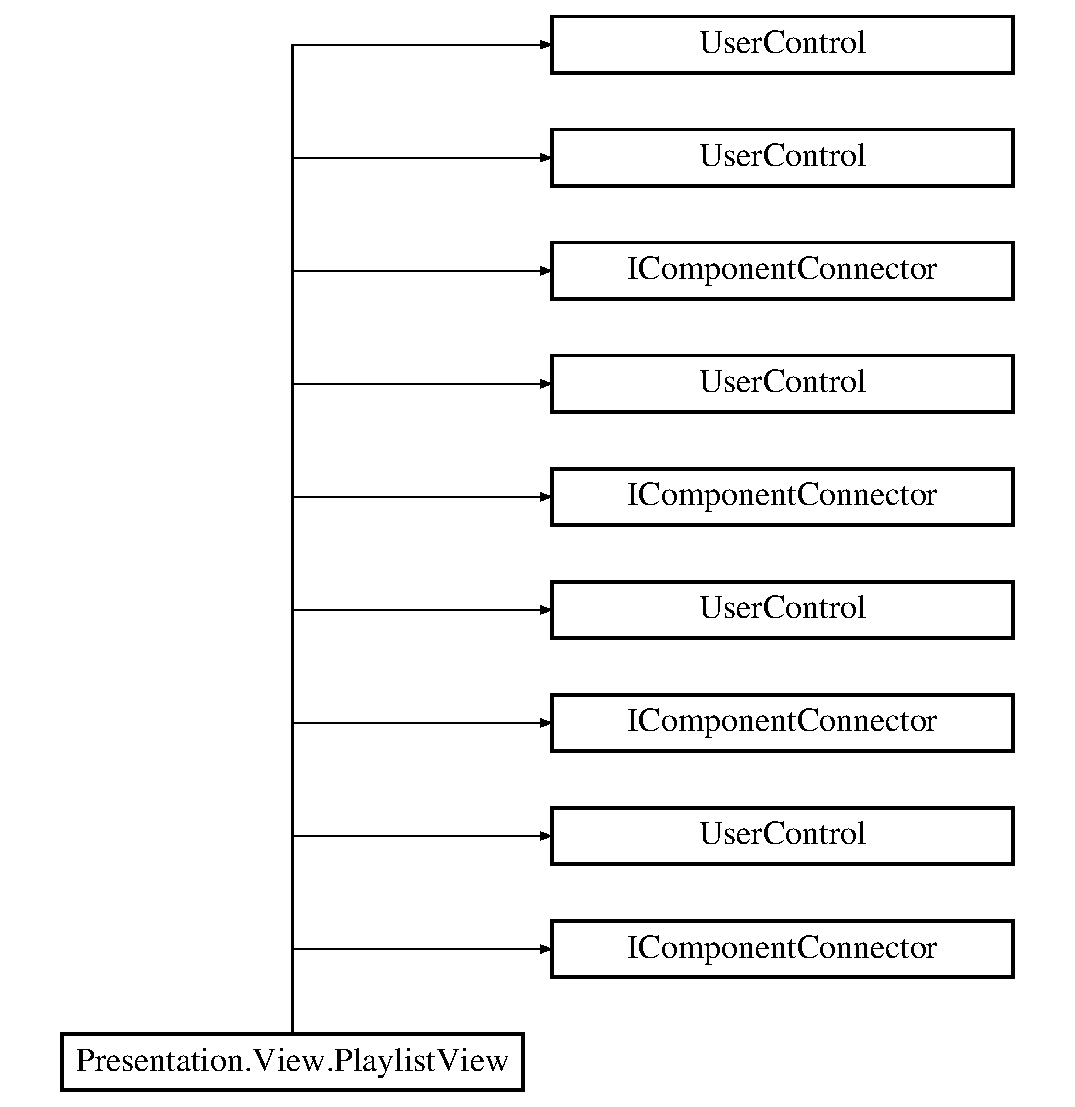
\includegraphics[height=10.000000cm]{class_presentation_1_1_view_1_1_playlist_view}
\end{center}
\end{figure}
\subsection*{Public Member Functions}
\begin{DoxyCompactItemize}
\item 
void \hyperlink{class_presentation_1_1_view_1_1_playlist_view_a025146640bbe45b42da5f72da40f3cc6}{Initialize\+Component} ()
\begin{DoxyCompactList}\small\item\em Initialize\+Component \end{DoxyCompactList}\item 
void \hyperlink{class_presentation_1_1_view_1_1_playlist_view_a025146640bbe45b42da5f72da40f3cc6}{Initialize\+Component} ()
\begin{DoxyCompactList}\small\item\em Initialize\+Component \end{DoxyCompactList}\item 
void \hyperlink{class_presentation_1_1_view_1_1_playlist_view_a025146640bbe45b42da5f72da40f3cc6}{Initialize\+Component} ()
\begin{DoxyCompactList}\small\item\em Initialize\+Component \end{DoxyCompactList}\item 
void \hyperlink{class_presentation_1_1_view_1_1_playlist_view_a025146640bbe45b42da5f72da40f3cc6}{Initialize\+Component} ()
\begin{DoxyCompactList}\small\item\em Initialize\+Component \end{DoxyCompactList}\end{DoxyCompactItemize}


\subsection{Detailed Description}
\hyperlink{class_presentation_1_1_view_1_1_playlist_view}{Playlist\+View} 

Interaction logic for Playlist\+View.\+xaml 

\subsection{Member Function Documentation}
\mbox{\Hypertarget{class_presentation_1_1_view_1_1_playlist_view_a025146640bbe45b42da5f72da40f3cc6}\label{class_presentation_1_1_view_1_1_playlist_view_a025146640bbe45b42da5f72da40f3cc6}} 
\index{Presentation\+::\+View\+::\+Playlist\+View@{Presentation\+::\+View\+::\+Playlist\+View}!Initialize\+Component@{Initialize\+Component}}
\index{Initialize\+Component@{Initialize\+Component}!Presentation\+::\+View\+::\+Playlist\+View@{Presentation\+::\+View\+::\+Playlist\+View}}
\subsubsection{\texorpdfstring{Initialize\+Component()}{InitializeComponent()}\hspace{0.1cm}{\footnotesize\ttfamily [1/4]}}
{\footnotesize\ttfamily void Presentation.\+View.\+Playlist\+View.\+Initialize\+Component (\begin{DoxyParamCaption}{ }\end{DoxyParamCaption})}



Initialize\+Component 

\mbox{\Hypertarget{class_presentation_1_1_view_1_1_playlist_view_a025146640bbe45b42da5f72da40f3cc6}\label{class_presentation_1_1_view_1_1_playlist_view_a025146640bbe45b42da5f72da40f3cc6}} 
\index{Presentation\+::\+View\+::\+Playlist\+View@{Presentation\+::\+View\+::\+Playlist\+View}!Initialize\+Component@{Initialize\+Component}}
\index{Initialize\+Component@{Initialize\+Component}!Presentation\+::\+View\+::\+Playlist\+View@{Presentation\+::\+View\+::\+Playlist\+View}}
\subsubsection{\texorpdfstring{Initialize\+Component()}{InitializeComponent()}\hspace{0.1cm}{\footnotesize\ttfamily [2/4]}}
{\footnotesize\ttfamily void Presentation.\+View.\+Playlist\+View.\+Initialize\+Component (\begin{DoxyParamCaption}{ }\end{DoxyParamCaption})}



Initialize\+Component 

\mbox{\Hypertarget{class_presentation_1_1_view_1_1_playlist_view_a025146640bbe45b42da5f72da40f3cc6}\label{class_presentation_1_1_view_1_1_playlist_view_a025146640bbe45b42da5f72da40f3cc6}} 
\index{Presentation\+::\+View\+::\+Playlist\+View@{Presentation\+::\+View\+::\+Playlist\+View}!Initialize\+Component@{Initialize\+Component}}
\index{Initialize\+Component@{Initialize\+Component}!Presentation\+::\+View\+::\+Playlist\+View@{Presentation\+::\+View\+::\+Playlist\+View}}
\subsubsection{\texorpdfstring{Initialize\+Component()}{InitializeComponent()}\hspace{0.1cm}{\footnotesize\ttfamily [3/4]}}
{\footnotesize\ttfamily void Presentation.\+View.\+Playlist\+View.\+Initialize\+Component (\begin{DoxyParamCaption}{ }\end{DoxyParamCaption})}



Initialize\+Component 

\mbox{\Hypertarget{class_presentation_1_1_view_1_1_playlist_view_a025146640bbe45b42da5f72da40f3cc6}\label{class_presentation_1_1_view_1_1_playlist_view_a025146640bbe45b42da5f72da40f3cc6}} 
\index{Presentation\+::\+View\+::\+Playlist\+View@{Presentation\+::\+View\+::\+Playlist\+View}!Initialize\+Component@{Initialize\+Component}}
\index{Initialize\+Component@{Initialize\+Component}!Presentation\+::\+View\+::\+Playlist\+View@{Presentation\+::\+View\+::\+Playlist\+View}}
\subsubsection{\texorpdfstring{Initialize\+Component()}{InitializeComponent()}\hspace{0.1cm}{\footnotesize\ttfamily [4/4]}}
{\footnotesize\ttfamily void Presentation.\+View.\+Playlist\+View.\+Initialize\+Component (\begin{DoxyParamCaption}{ }\end{DoxyParamCaption})}



Initialize\+Component 



The documentation for this class was generated from the following files\+:\begin{DoxyCompactItemize}
\item 
C\+:/\+W\+O\+R\+K\+S\+P\+A\+C\+E/\+T\+P\+I-\/end/\+Gestion\+Audio/\+Gestion\+Audio/obj/\+Debug/\+View/Playlist\+View.\+g.\+cs\item 
C\+:/\+W\+O\+R\+K\+S\+P\+A\+C\+E/\+T\+P\+I-\/end/\+Gestion\+Audio/\+Gestion\+Audio/obj/\+Debug/\+View/Playlist\+View.\+g.\+i.\+cs\item 
C\+:/\+W\+O\+R\+K\+S\+P\+A\+C\+E/\+T\+P\+I-\/end/\+Gestion\+Audio/\+Gestion\+Audio/\+View/Playlist\+View.\+xaml.\+cs\end{DoxyCompactItemize}

\hypertarget{class_presentation_1_1_view_model_1_1_playlist_view_model}{}\section{Presentation.\+View\+Model.\+Playlist\+View\+Model Class Reference}
\label{class_presentation_1_1_view_model_1_1_playlist_view_model}\index{Presentation.\+View\+Model.\+Playlist\+View\+Model@{Presentation.\+View\+Model.\+Playlist\+View\+Model}}


This class contain the logic for the playlistview  


Inheritance diagram for Presentation.\+View\+Model.\+Playlist\+View\+Model\+:\begin{figure}[H]
\begin{center}
\leavevmode
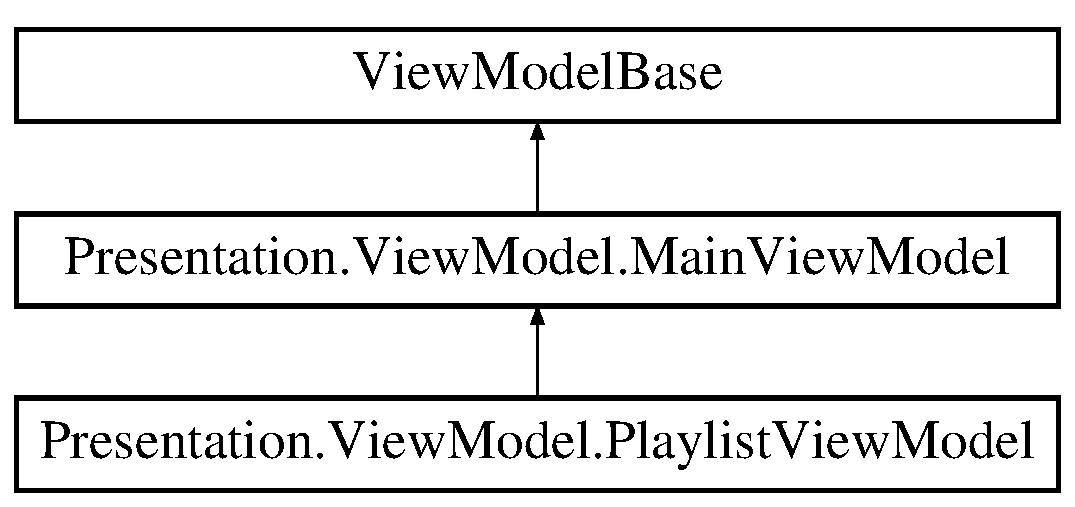
\includegraphics[height=3.000000cm]{class_presentation_1_1_view_model_1_1_playlist_view_model}
\end{center}
\end{figure}
\subsection*{Public Member Functions}
\begin{DoxyCompactItemize}
\item 
\hyperlink{class_presentation_1_1_view_model_1_1_playlist_view_model_a2465d55b6ed6c3de83bd1547fb95e1a3}{Playlist\+View\+Model} ()
\begin{DoxyCompactList}\small\item\em Set playlists \end{DoxyCompactList}\item 
async Task$<$ \hyperlink{class_d_t_o_1_1_entity_1_1_playlist}{Playlist} $>$ \hyperlink{class_presentation_1_1_view_model_1_1_playlist_view_model_a3f24674bdebf1cd67215ed847eb39624}{Click\+Add} ()
\begin{DoxyCompactList}\small\item\em When the user click to add a playlist \end{DoxyCompactList}\item 
void \hyperlink{class_presentation_1_1_view_model_1_1_playlist_view_model_aca79c8f84c21bfe3c1ab2cc48c1cc76f}{Click\+Remove} ()
\begin{DoxyCompactList}\small\item\em When the user click to remove a playlist \end{DoxyCompactList}\item 
void \hyperlink{class_presentation_1_1_view_model_1_1_playlist_view_model_a251fc433a805e640e40769120160b645}{Update\+Playlist} ()
\begin{DoxyCompactList}\small\item\em Update all the playlists elements \end{DoxyCompactList}\end{DoxyCompactItemize}
\subsection*{Properties}
\begin{DoxyCompactItemize}
\item 
\mbox{\Hypertarget{class_presentation_1_1_view_model_1_1_playlist_view_model_a3b228cd7d10f6082d7695b8227a0ef72}\label{class_presentation_1_1_view_model_1_1_playlist_view_model_a3b228cd7d10f6082d7695b8227a0ef72}} 
\hyperlink{class_presentation_1_1_view_model_1_1_music_view_model}{Music\+View\+Model} {\bfseries Music\+View\+Model}\hspace{0.3cm}{\ttfamily  \mbox{[}get, set\mbox{]}}
\item 
\mbox{\Hypertarget{class_presentation_1_1_view_model_1_1_playlist_view_model_ae8f4ccb5efdebeb604c94faf9c098fec}\label{class_presentation_1_1_view_model_1_1_playlist_view_model_ae8f4ccb5efdebeb604c94faf9c098fec}} 
Relay\+Command {\bfseries On\+Click\+Add}\hspace{0.3cm}{\ttfamily  \mbox{[}get, set\mbox{]}}
\item 
\mbox{\Hypertarget{class_presentation_1_1_view_model_1_1_playlist_view_model_a617dbf3a65c5e57d113bb97e97c133a4}\label{class_presentation_1_1_view_model_1_1_playlist_view_model_a617dbf3a65c5e57d113bb97e97c133a4}} 
Relay\+Command {\bfseries On\+Click\+Remove}\hspace{0.3cm}{\ttfamily  \mbox{[}get, set\mbox{]}}
\item 
\mbox{\Hypertarget{class_presentation_1_1_view_model_1_1_playlist_view_model_a8753d157677e9d8bf913bb50429037ba}\label{class_presentation_1_1_view_model_1_1_playlist_view_model_a8753d157677e9d8bf913bb50429037ba}} 
Observable\+Collection$<$ \hyperlink{class_d_t_o_1_1_entity_1_1_playlist}{Playlist} $>$ {\bfseries Playlists}\hspace{0.3cm}{\ttfamily  \mbox{[}get, set\mbox{]}}
\item 
\mbox{\Hypertarget{class_presentation_1_1_view_model_1_1_playlist_view_model_a5552b61d284f35b3d74d7f3a6a79c4e3}\label{class_presentation_1_1_view_model_1_1_playlist_view_model_a5552b61d284f35b3d74d7f3a6a79c4e3}} 
\hyperlink{class_d_t_o_1_1_entity_1_1_playlist}{Playlist} {\bfseries Selected\+Item}\hspace{0.3cm}{\ttfamily  \mbox{[}get, set\mbox{]}}
\end{DoxyCompactItemize}


\subsection{Detailed Description}
This class contain the logic for the playlistview 



\subsection{Constructor \& Destructor Documentation}
\mbox{\Hypertarget{class_presentation_1_1_view_model_1_1_playlist_view_model_a2465d55b6ed6c3de83bd1547fb95e1a3}\label{class_presentation_1_1_view_model_1_1_playlist_view_model_a2465d55b6ed6c3de83bd1547fb95e1a3}} 
\index{Presentation\+::\+View\+Model\+::\+Playlist\+View\+Model@{Presentation\+::\+View\+Model\+::\+Playlist\+View\+Model}!Playlist\+View\+Model@{Playlist\+View\+Model}}
\index{Playlist\+View\+Model@{Playlist\+View\+Model}!Presentation\+::\+View\+Model\+::\+Playlist\+View\+Model@{Presentation\+::\+View\+Model\+::\+Playlist\+View\+Model}}
\subsubsection{\texorpdfstring{Playlist\+View\+Model()}{PlaylistViewModel()}}
{\footnotesize\ttfamily Presentation.\+View\+Model.\+Playlist\+View\+Model.\+Playlist\+View\+Model (\begin{DoxyParamCaption}{ }\end{DoxyParamCaption})}



Set playlists 



\subsection{Member Function Documentation}
\mbox{\Hypertarget{class_presentation_1_1_view_model_1_1_playlist_view_model_a3f24674bdebf1cd67215ed847eb39624}\label{class_presentation_1_1_view_model_1_1_playlist_view_model_a3f24674bdebf1cd67215ed847eb39624}} 
\index{Presentation\+::\+View\+Model\+::\+Playlist\+View\+Model@{Presentation\+::\+View\+Model\+::\+Playlist\+View\+Model}!Click\+Add@{Click\+Add}}
\index{Click\+Add@{Click\+Add}!Presentation\+::\+View\+Model\+::\+Playlist\+View\+Model@{Presentation\+::\+View\+Model\+::\+Playlist\+View\+Model}}
\subsubsection{\texorpdfstring{Click\+Add()}{ClickAdd()}}
{\footnotesize\ttfamily async Task$<$\hyperlink{class_d_t_o_1_1_entity_1_1_playlist}{Playlist}$>$ Presentation.\+View\+Model.\+Playlist\+View\+Model.\+Click\+Add (\begin{DoxyParamCaption}{ }\end{DoxyParamCaption})}



When the user click to add a playlist 

\mbox{\Hypertarget{class_presentation_1_1_view_model_1_1_playlist_view_model_aca79c8f84c21bfe3c1ab2cc48c1cc76f}\label{class_presentation_1_1_view_model_1_1_playlist_view_model_aca79c8f84c21bfe3c1ab2cc48c1cc76f}} 
\index{Presentation\+::\+View\+Model\+::\+Playlist\+View\+Model@{Presentation\+::\+View\+Model\+::\+Playlist\+View\+Model}!Click\+Remove@{Click\+Remove}}
\index{Click\+Remove@{Click\+Remove}!Presentation\+::\+View\+Model\+::\+Playlist\+View\+Model@{Presentation\+::\+View\+Model\+::\+Playlist\+View\+Model}}
\subsubsection{\texorpdfstring{Click\+Remove()}{ClickRemove()}}
{\footnotesize\ttfamily void Presentation.\+View\+Model.\+Playlist\+View\+Model.\+Click\+Remove (\begin{DoxyParamCaption}{ }\end{DoxyParamCaption})}



When the user click to remove a playlist 

\mbox{\Hypertarget{class_presentation_1_1_view_model_1_1_playlist_view_model_a251fc433a805e640e40769120160b645}\label{class_presentation_1_1_view_model_1_1_playlist_view_model_a251fc433a805e640e40769120160b645}} 
\index{Presentation\+::\+View\+Model\+::\+Playlist\+View\+Model@{Presentation\+::\+View\+Model\+::\+Playlist\+View\+Model}!Update\+Playlist@{Update\+Playlist}}
\index{Update\+Playlist@{Update\+Playlist}!Presentation\+::\+View\+Model\+::\+Playlist\+View\+Model@{Presentation\+::\+View\+Model\+::\+Playlist\+View\+Model}}
\subsubsection{\texorpdfstring{Update\+Playlist()}{UpdatePlaylist()}}
{\footnotesize\ttfamily void Presentation.\+View\+Model.\+Playlist\+View\+Model.\+Update\+Playlist (\begin{DoxyParamCaption}{ }\end{DoxyParamCaption})}



Update all the playlists elements 



The documentation for this class was generated from the following file\+:\begin{DoxyCompactItemize}
\item 
C\+:/\+W\+O\+R\+K\+S\+P\+A\+C\+E/\+T\+P\+I-\/end/\+Gestion\+Audio/\+Gestion\+Audio/\+View\+Model/Playlist\+View\+Model.\+cs\end{DoxyCompactItemize}

\hypertarget{class_presentation_1_1_view_1_1_flyout_1_1_property_flyout_view}{}\section{Presentation.\+View.\+Flyout.\+Property\+Flyout\+View Class Reference}
\label{class_presentation_1_1_view_1_1_flyout_1_1_property_flyout_view}\index{Presentation.\+View.\+Flyout.\+Property\+Flyout\+View@{Presentation.\+View.\+Flyout.\+Property\+Flyout\+View}}


\hyperlink{class_presentation_1_1_view_1_1_flyout_1_1_property_flyout_view}{Property\+Flyout\+View}  


Inheritance diagram for Presentation.\+View.\+Flyout.\+Property\+Flyout\+View\+:\begin{figure}[H]
\begin{center}
\leavevmode
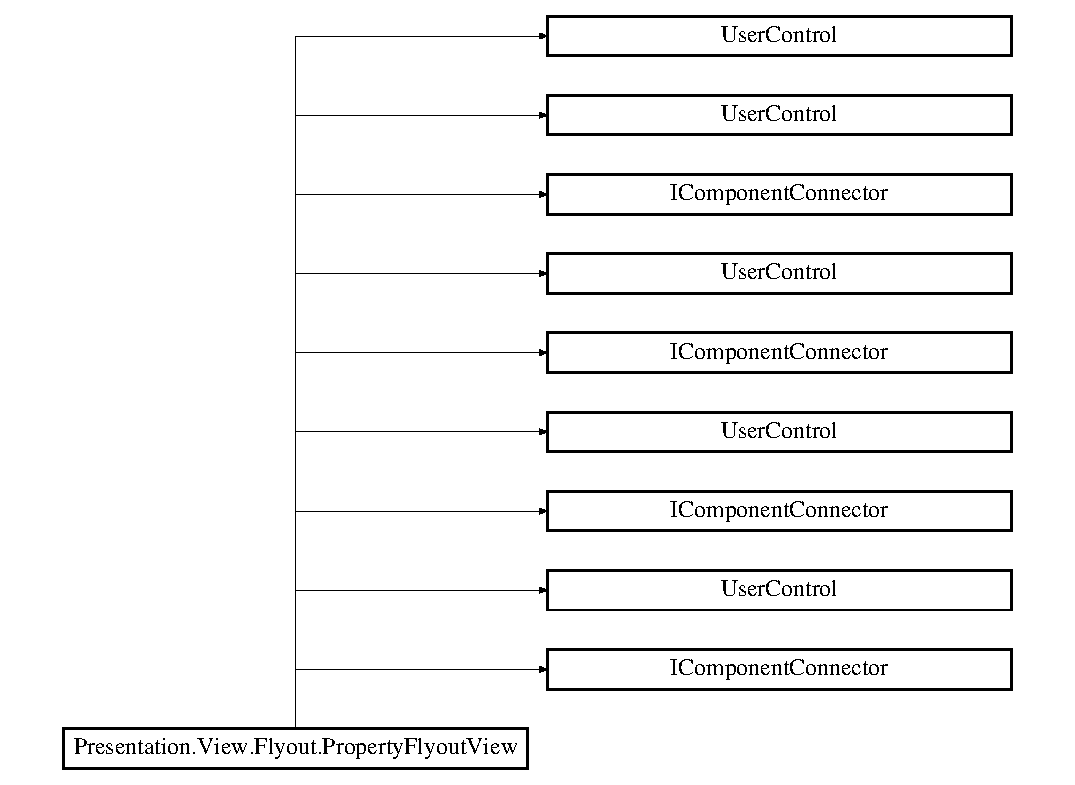
\includegraphics[height=10.000000cm]{class_presentation_1_1_view_1_1_flyout_1_1_property_flyout_view}
\end{center}
\end{figure}
\subsection*{Public Member Functions}
\begin{DoxyCompactItemize}
\item 
void \hyperlink{class_presentation_1_1_view_1_1_flyout_1_1_property_flyout_view_a9b44c10f88d02a145b30b550ebfbf1ac}{Initialize\+Component} ()
\begin{DoxyCompactList}\small\item\em Initialize\+Component \end{DoxyCompactList}\item 
void \hyperlink{class_presentation_1_1_view_1_1_flyout_1_1_property_flyout_view_a9b44c10f88d02a145b30b550ebfbf1ac}{Initialize\+Component} ()
\begin{DoxyCompactList}\small\item\em Initialize\+Component \end{DoxyCompactList}\item 
void \hyperlink{class_presentation_1_1_view_1_1_flyout_1_1_property_flyout_view_a9b44c10f88d02a145b30b550ebfbf1ac}{Initialize\+Component} ()
\begin{DoxyCompactList}\small\item\em Initialize\+Component \end{DoxyCompactList}\item 
void \hyperlink{class_presentation_1_1_view_1_1_flyout_1_1_property_flyout_view_a9b44c10f88d02a145b30b550ebfbf1ac}{Initialize\+Component} ()
\begin{DoxyCompactList}\small\item\em Initialize\+Component \end{DoxyCompactList}\end{DoxyCompactItemize}


\subsection{Detailed Description}
\hyperlink{class_presentation_1_1_view_1_1_flyout_1_1_property_flyout_view}{Property\+Flyout\+View} 

Interaction logic for Property\+Flyout\+View.\+xaml 

\subsection{Member Function Documentation}
\mbox{\Hypertarget{class_presentation_1_1_view_1_1_flyout_1_1_property_flyout_view_a9b44c10f88d02a145b30b550ebfbf1ac}\label{class_presentation_1_1_view_1_1_flyout_1_1_property_flyout_view_a9b44c10f88d02a145b30b550ebfbf1ac}} 
\index{Presentation\+::\+View\+::\+Flyout\+::\+Property\+Flyout\+View@{Presentation\+::\+View\+::\+Flyout\+::\+Property\+Flyout\+View}!Initialize\+Component@{Initialize\+Component}}
\index{Initialize\+Component@{Initialize\+Component}!Presentation\+::\+View\+::\+Flyout\+::\+Property\+Flyout\+View@{Presentation\+::\+View\+::\+Flyout\+::\+Property\+Flyout\+View}}
\subsubsection{\texorpdfstring{Initialize\+Component()}{InitializeComponent()}\hspace{0.1cm}{\footnotesize\ttfamily [1/4]}}
{\footnotesize\ttfamily void Presentation.\+View.\+Flyout.\+Property\+Flyout\+View.\+Initialize\+Component (\begin{DoxyParamCaption}{ }\end{DoxyParamCaption})}



Initialize\+Component 

\mbox{\Hypertarget{class_presentation_1_1_view_1_1_flyout_1_1_property_flyout_view_a9b44c10f88d02a145b30b550ebfbf1ac}\label{class_presentation_1_1_view_1_1_flyout_1_1_property_flyout_view_a9b44c10f88d02a145b30b550ebfbf1ac}} 
\index{Presentation\+::\+View\+::\+Flyout\+::\+Property\+Flyout\+View@{Presentation\+::\+View\+::\+Flyout\+::\+Property\+Flyout\+View}!Initialize\+Component@{Initialize\+Component}}
\index{Initialize\+Component@{Initialize\+Component}!Presentation\+::\+View\+::\+Flyout\+::\+Property\+Flyout\+View@{Presentation\+::\+View\+::\+Flyout\+::\+Property\+Flyout\+View}}
\subsubsection{\texorpdfstring{Initialize\+Component()}{InitializeComponent()}\hspace{0.1cm}{\footnotesize\ttfamily [2/4]}}
{\footnotesize\ttfamily void Presentation.\+View.\+Flyout.\+Property\+Flyout\+View.\+Initialize\+Component (\begin{DoxyParamCaption}{ }\end{DoxyParamCaption})}



Initialize\+Component 

\mbox{\Hypertarget{class_presentation_1_1_view_1_1_flyout_1_1_property_flyout_view_a9b44c10f88d02a145b30b550ebfbf1ac}\label{class_presentation_1_1_view_1_1_flyout_1_1_property_flyout_view_a9b44c10f88d02a145b30b550ebfbf1ac}} 
\index{Presentation\+::\+View\+::\+Flyout\+::\+Property\+Flyout\+View@{Presentation\+::\+View\+::\+Flyout\+::\+Property\+Flyout\+View}!Initialize\+Component@{Initialize\+Component}}
\index{Initialize\+Component@{Initialize\+Component}!Presentation\+::\+View\+::\+Flyout\+::\+Property\+Flyout\+View@{Presentation\+::\+View\+::\+Flyout\+::\+Property\+Flyout\+View}}
\subsubsection{\texorpdfstring{Initialize\+Component()}{InitializeComponent()}\hspace{0.1cm}{\footnotesize\ttfamily [3/4]}}
{\footnotesize\ttfamily void Presentation.\+View.\+Flyout.\+Property\+Flyout\+View.\+Initialize\+Component (\begin{DoxyParamCaption}{ }\end{DoxyParamCaption})}



Initialize\+Component 

\mbox{\Hypertarget{class_presentation_1_1_view_1_1_flyout_1_1_property_flyout_view_a9b44c10f88d02a145b30b550ebfbf1ac}\label{class_presentation_1_1_view_1_1_flyout_1_1_property_flyout_view_a9b44c10f88d02a145b30b550ebfbf1ac}} 
\index{Presentation\+::\+View\+::\+Flyout\+::\+Property\+Flyout\+View@{Presentation\+::\+View\+::\+Flyout\+::\+Property\+Flyout\+View}!Initialize\+Component@{Initialize\+Component}}
\index{Initialize\+Component@{Initialize\+Component}!Presentation\+::\+View\+::\+Flyout\+::\+Property\+Flyout\+View@{Presentation\+::\+View\+::\+Flyout\+::\+Property\+Flyout\+View}}
\subsubsection{\texorpdfstring{Initialize\+Component()}{InitializeComponent()}\hspace{0.1cm}{\footnotesize\ttfamily [4/4]}}
{\footnotesize\ttfamily void Presentation.\+View.\+Flyout.\+Property\+Flyout\+View.\+Initialize\+Component (\begin{DoxyParamCaption}{ }\end{DoxyParamCaption})}



Initialize\+Component 



The documentation for this class was generated from the following files\+:\begin{DoxyCompactItemize}
\item 
C\+:/\+W\+O\+R\+K\+S\+P\+A\+C\+E/\+T\+P\+I-\/end/\+Gestion\+Audio/\+Gestion\+Audio/obj/\+Debug/\+View/\+Flyout/Property\+Flyout\+View.\+g.\+cs\item 
C\+:/\+W\+O\+R\+K\+S\+P\+A\+C\+E/\+T\+P\+I-\/end/\+Gestion\+Audio/\+Gestion\+Audio/obj/\+Debug/\+View/\+Flyout/Property\+Flyout\+View.\+g.\+i.\+cs\item 
C\+:/\+W\+O\+R\+K\+S\+P\+A\+C\+E/\+T\+P\+I-\/end/\+Gestion\+Audio/\+Gestion\+Audio/\+View/\+Flyout/Property\+Flyout\+View.\+xaml.\+cs\end{DoxyCompactItemize}

\hypertarget{class_d_t_o_1_1_entity_1_1_radio}{}\section{D\+T\+O.\+Entity.\+Radio Class Reference}
\label{class_d_t_o_1_1_entity_1_1_radio}\index{D\+T\+O.\+Entity.\+Radio@{D\+T\+O.\+Entity.\+Radio}}


The database \hyperlink{class_d_t_o_1_1_entity_1_1_radio}{Radio} entity  


Inheritance diagram for D\+T\+O.\+Entity.\+Radio\+:\begin{figure}[H]
\begin{center}
\leavevmode
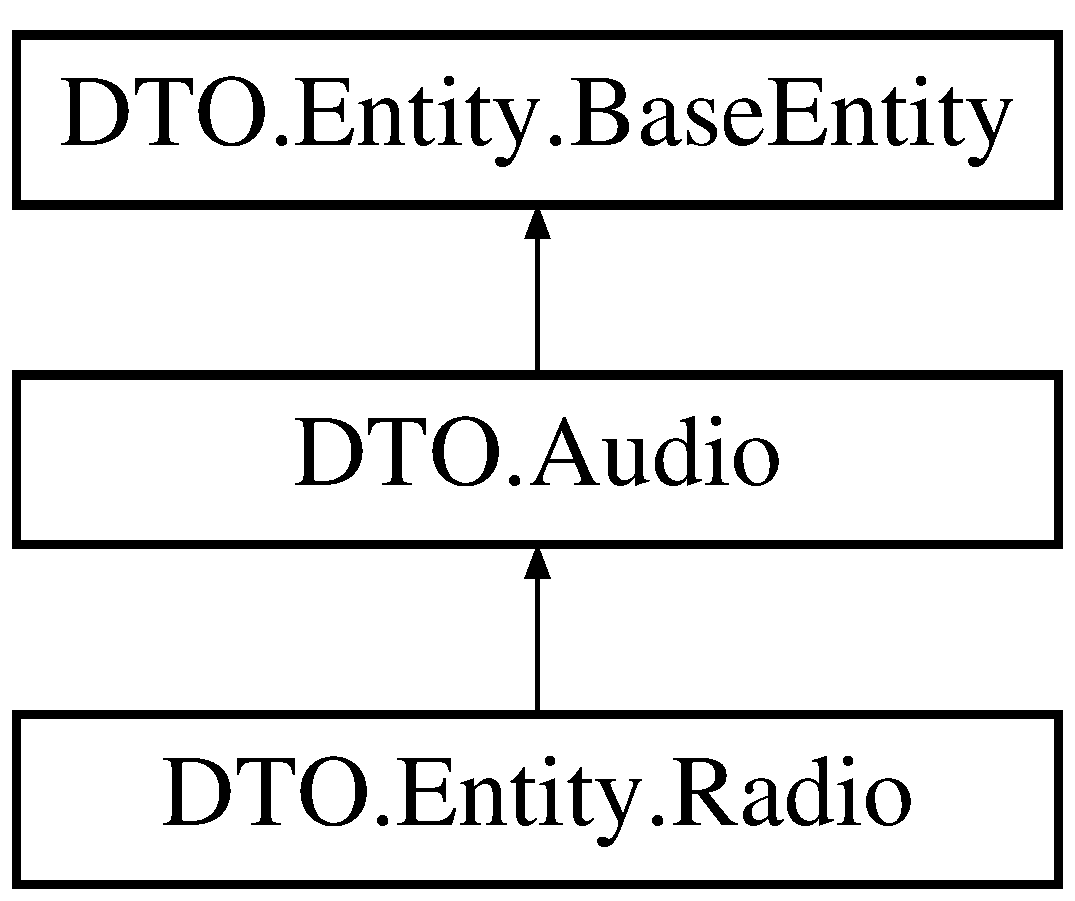
\includegraphics[height=3.000000cm]{class_d_t_o_1_1_entity_1_1_radio}
\end{center}
\end{figure}
\subsection*{Properties}
\begin{DoxyCompactItemize}
\item 
\mbox{\Hypertarget{class_d_t_o_1_1_entity_1_1_radio_ab80dc33afc8151c08566e75339db6bff}\label{class_d_t_o_1_1_entity_1_1_radio_ab80dc33afc8151c08566e75339db6bff}} 
string {\bfseries Desrciption}\hspace{0.3cm}{\ttfamily  \mbox{[}get, set\mbox{]}}
\item 
\mbox{\Hypertarget{class_d_t_o_1_1_entity_1_1_radio_aac2ea4fe421d2c670aa6ac3aea303099}\label{class_d_t_o_1_1_entity_1_1_radio_aac2ea4fe421d2c670aa6ac3aea303099}} 
string {\bfseries Format}\hspace{0.3cm}{\ttfamily  \mbox{[}get, set\mbox{]}}
\item 
\mbox{\Hypertarget{class_d_t_o_1_1_entity_1_1_radio_a61e46a47f085108803bac41a15480903}\label{class_d_t_o_1_1_entity_1_1_radio_a61e46a47f085108803bac41a15480903}} 
Date\+Time {\bfseries Last\+Listen}\hspace{0.3cm}{\ttfamily  \mbox{[}get, set\mbox{]}}
\item 
\mbox{\Hypertarget{class_d_t_o_1_1_entity_1_1_radio_a352479e427140066b624ac5902ace21f}\label{class_d_t_o_1_1_entity_1_1_radio_a352479e427140066b624ac5902ace21f}} 
string {\bfseries Logo\+Url}\hspace{0.3cm}{\ttfamily  \mbox{[}get, set\mbox{]}}
\item 
\mbox{\Hypertarget{class_d_t_o_1_1_entity_1_1_radio_a081993b6d85580f5c85cc11bc4f5356c}\label{class_d_t_o_1_1_entity_1_1_radio_a081993b6d85580f5c85cc11bc4f5356c}} 
string {\bfseries Shout\+Cast\+Id}\hspace{0.3cm}{\ttfamily  \mbox{[}get, set\mbox{]}}
\end{DoxyCompactItemize}
\subsection*{Additional Inherited Members}


\subsection{Detailed Description}
The database \hyperlink{class_d_t_o_1_1_entity_1_1_radio}{Radio} entity 



The documentation for this class was generated from the following file\+:\begin{DoxyCompactItemize}
\item 
C\+:/\+W\+O\+R\+K\+S\+P\+A\+C\+E/\+T\+P\+I-\/end/\+Gestion\+Audio/\+D\+T\+O/\+Entity/Radio.\+cs\end{DoxyCompactItemize}

\hypertarget{class_presentation_1_1_view_1_1_list_1_1_radio_list_view}{}\section{Presentation.\+View.\+List.\+Radio\+List\+View Class Reference}
\label{class_presentation_1_1_view_1_1_list_1_1_radio_list_view}\index{Presentation.\+View.\+List.\+Radio\+List\+View@{Presentation.\+View.\+List.\+Radio\+List\+View}}


\hyperlink{class_presentation_1_1_view_1_1_list_1_1_radio_list_view}{Radio\+List\+View}  


Inheritance diagram for Presentation.\+View.\+List.\+Radio\+List\+View\+:\begin{figure}[H]
\begin{center}
\leavevmode
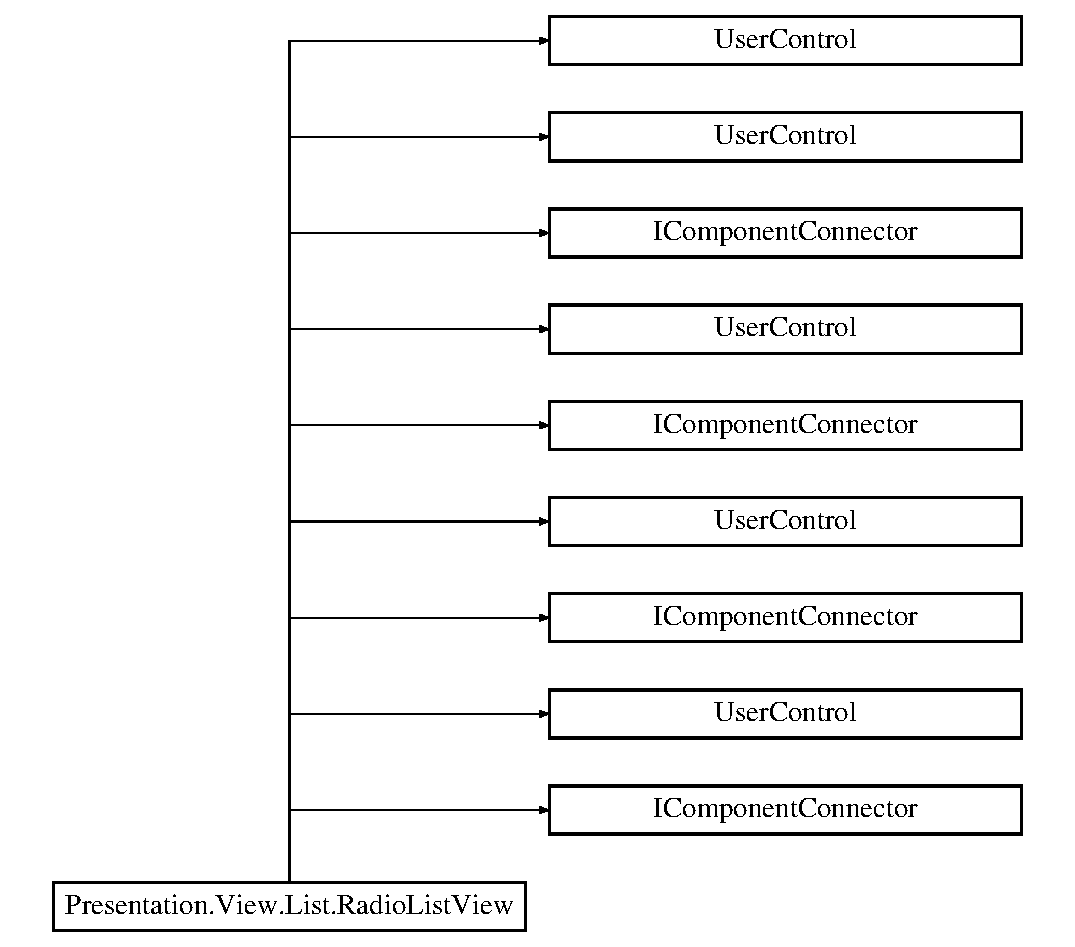
\includegraphics[height=10.000000cm]{class_presentation_1_1_view_1_1_list_1_1_radio_list_view}
\end{center}
\end{figure}
\subsection*{Public Member Functions}
\begin{DoxyCompactItemize}
\item 
void \hyperlink{class_presentation_1_1_view_1_1_list_1_1_radio_list_view_a66633fd5cb1527cc49439c458bdd6ed8}{Initialize\+Component} ()
\begin{DoxyCompactList}\small\item\em Initialize\+Component \end{DoxyCompactList}\item 
void \hyperlink{class_presentation_1_1_view_1_1_list_1_1_radio_list_view_a66633fd5cb1527cc49439c458bdd6ed8}{Initialize\+Component} ()
\begin{DoxyCompactList}\small\item\em Initialize\+Component \end{DoxyCompactList}\item 
void \hyperlink{class_presentation_1_1_view_1_1_list_1_1_radio_list_view_a66633fd5cb1527cc49439c458bdd6ed8}{Initialize\+Component} ()
\begin{DoxyCompactList}\small\item\em Initialize\+Component \end{DoxyCompactList}\item 
void \hyperlink{class_presentation_1_1_view_1_1_list_1_1_radio_list_view_a66633fd5cb1527cc49439c458bdd6ed8}{Initialize\+Component} ()
\begin{DoxyCompactList}\small\item\em Initialize\+Component \end{DoxyCompactList}\end{DoxyCompactItemize}


\subsection{Detailed Description}
\hyperlink{class_presentation_1_1_view_1_1_list_1_1_radio_list_view}{Radio\+List\+View} 

Interaction logic for Music\+Home.\+xaml 

\subsection{Member Function Documentation}
\mbox{\Hypertarget{class_presentation_1_1_view_1_1_list_1_1_radio_list_view_a66633fd5cb1527cc49439c458bdd6ed8}\label{class_presentation_1_1_view_1_1_list_1_1_radio_list_view_a66633fd5cb1527cc49439c458bdd6ed8}} 
\index{Presentation\+::\+View\+::\+List\+::\+Radio\+List\+View@{Presentation\+::\+View\+::\+List\+::\+Radio\+List\+View}!Initialize\+Component@{Initialize\+Component}}
\index{Initialize\+Component@{Initialize\+Component}!Presentation\+::\+View\+::\+List\+::\+Radio\+List\+View@{Presentation\+::\+View\+::\+List\+::\+Radio\+List\+View}}
\subsubsection{\texorpdfstring{Initialize\+Component()}{InitializeComponent()}\hspace{0.1cm}{\footnotesize\ttfamily [1/4]}}
{\footnotesize\ttfamily void Presentation.\+View.\+List.\+Radio\+List\+View.\+Initialize\+Component (\begin{DoxyParamCaption}{ }\end{DoxyParamCaption})}



Initialize\+Component 

\mbox{\Hypertarget{class_presentation_1_1_view_1_1_list_1_1_radio_list_view_a66633fd5cb1527cc49439c458bdd6ed8}\label{class_presentation_1_1_view_1_1_list_1_1_radio_list_view_a66633fd5cb1527cc49439c458bdd6ed8}} 
\index{Presentation\+::\+View\+::\+List\+::\+Radio\+List\+View@{Presentation\+::\+View\+::\+List\+::\+Radio\+List\+View}!Initialize\+Component@{Initialize\+Component}}
\index{Initialize\+Component@{Initialize\+Component}!Presentation\+::\+View\+::\+List\+::\+Radio\+List\+View@{Presentation\+::\+View\+::\+List\+::\+Radio\+List\+View}}
\subsubsection{\texorpdfstring{Initialize\+Component()}{InitializeComponent()}\hspace{0.1cm}{\footnotesize\ttfamily [2/4]}}
{\footnotesize\ttfamily void Presentation.\+View.\+List.\+Radio\+List\+View.\+Initialize\+Component (\begin{DoxyParamCaption}{ }\end{DoxyParamCaption})}



Initialize\+Component 

\mbox{\Hypertarget{class_presentation_1_1_view_1_1_list_1_1_radio_list_view_a66633fd5cb1527cc49439c458bdd6ed8}\label{class_presentation_1_1_view_1_1_list_1_1_radio_list_view_a66633fd5cb1527cc49439c458bdd6ed8}} 
\index{Presentation\+::\+View\+::\+List\+::\+Radio\+List\+View@{Presentation\+::\+View\+::\+List\+::\+Radio\+List\+View}!Initialize\+Component@{Initialize\+Component}}
\index{Initialize\+Component@{Initialize\+Component}!Presentation\+::\+View\+::\+List\+::\+Radio\+List\+View@{Presentation\+::\+View\+::\+List\+::\+Radio\+List\+View}}
\subsubsection{\texorpdfstring{Initialize\+Component()}{InitializeComponent()}\hspace{0.1cm}{\footnotesize\ttfamily [3/4]}}
{\footnotesize\ttfamily void Presentation.\+View.\+List.\+Radio\+List\+View.\+Initialize\+Component (\begin{DoxyParamCaption}{ }\end{DoxyParamCaption})}



Initialize\+Component 

\mbox{\Hypertarget{class_presentation_1_1_view_1_1_list_1_1_radio_list_view_a66633fd5cb1527cc49439c458bdd6ed8}\label{class_presentation_1_1_view_1_1_list_1_1_radio_list_view_a66633fd5cb1527cc49439c458bdd6ed8}} 
\index{Presentation\+::\+View\+::\+List\+::\+Radio\+List\+View@{Presentation\+::\+View\+::\+List\+::\+Radio\+List\+View}!Initialize\+Component@{Initialize\+Component}}
\index{Initialize\+Component@{Initialize\+Component}!Presentation\+::\+View\+::\+List\+::\+Radio\+List\+View@{Presentation\+::\+View\+::\+List\+::\+Radio\+List\+View}}
\subsubsection{\texorpdfstring{Initialize\+Component()}{InitializeComponent()}\hspace{0.1cm}{\footnotesize\ttfamily [4/4]}}
{\footnotesize\ttfamily void Presentation.\+View.\+List.\+Radio\+List\+View.\+Initialize\+Component (\begin{DoxyParamCaption}{ }\end{DoxyParamCaption})}



Initialize\+Component 



The documentation for this class was generated from the following files\+:\begin{DoxyCompactItemize}
\item 
C\+:/\+W\+O\+R\+K\+S\+P\+A\+C\+E/\+T\+P\+I-\/end/\+Gestion\+Audio/\+Gestion\+Audio/obj/\+Debug/\+View/\+List/Radio\+List\+View.\+g.\+cs\item 
C\+:/\+W\+O\+R\+K\+S\+P\+A\+C\+E/\+T\+P\+I-\/end/\+Gestion\+Audio/\+Gestion\+Audio/obj/\+Debug/\+View/\+List/Radio\+List\+View.\+g.\+i.\+cs\item 
C\+:/\+W\+O\+R\+K\+S\+P\+A\+C\+E/\+T\+P\+I-\/end/\+Gestion\+Audio/\+Gestion\+Audio/\+View/\+List/Radio\+List\+View.\+xaml.\+cs\end{DoxyCompactItemize}

\hypertarget{class_unit_test_1_1_radio_test}{}\section{Unit\+Test.\+Radio\+Test Class Reference}
\label{class_unit_test_1_1_radio_test}\index{Unit\+Test.\+Radio\+Test@{Unit\+Test.\+Radio\+Test}}


Contain all test to make the radios work  


\subsection*{Public Member Functions}
\begin{DoxyCompactItemize}
\item 
void \hyperlink{class_unit_test_1_1_radio_test_a3f01b868a994c15be119989a8cc67f41}{Check\+Api\+Connection} ()
\begin{DoxyCompactList}\small\item\em Try to initialize an A\+PI connection \end{DoxyCompactList}\item 
void \hyperlink{class_unit_test_1_1_radio_test_aef2bff78a59914b1c75dc01013fa8d1a}{Check\+Api\+Data} ()
\begin{DoxyCompactList}\small\item\em Make a search in the api \end{DoxyCompactList}\item 
void \hyperlink{class_unit_test_1_1_radio_test_a3616a2504096bca4385994eee11aa116}{Check\+Radio\+Info} ()
\begin{DoxyCompactList}\small\item\em Check that the data I got from the api is the one I was looking for \end{DoxyCompactList}\end{DoxyCompactItemize}


\subsection{Detailed Description}
Contain all test to make the radios work 



\subsection{Member Function Documentation}
\mbox{\Hypertarget{class_unit_test_1_1_radio_test_a3f01b868a994c15be119989a8cc67f41}\label{class_unit_test_1_1_radio_test_a3f01b868a994c15be119989a8cc67f41}} 
\index{Unit\+Test\+::\+Radio\+Test@{Unit\+Test\+::\+Radio\+Test}!Check\+Api\+Connection@{Check\+Api\+Connection}}
\index{Check\+Api\+Connection@{Check\+Api\+Connection}!Unit\+Test\+::\+Radio\+Test@{Unit\+Test\+::\+Radio\+Test}}
\subsubsection{\texorpdfstring{Check\+Api\+Connection()}{CheckApiConnection()}}
{\footnotesize\ttfamily void Unit\+Test.\+Radio\+Test.\+Check\+Api\+Connection (\begin{DoxyParamCaption}{ }\end{DoxyParamCaption})}



Try to initialize an A\+PI connection 

\mbox{\Hypertarget{class_unit_test_1_1_radio_test_aef2bff78a59914b1c75dc01013fa8d1a}\label{class_unit_test_1_1_radio_test_aef2bff78a59914b1c75dc01013fa8d1a}} 
\index{Unit\+Test\+::\+Radio\+Test@{Unit\+Test\+::\+Radio\+Test}!Check\+Api\+Data@{Check\+Api\+Data}}
\index{Check\+Api\+Data@{Check\+Api\+Data}!Unit\+Test\+::\+Radio\+Test@{Unit\+Test\+::\+Radio\+Test}}
\subsubsection{\texorpdfstring{Check\+Api\+Data()}{CheckApiData()}}
{\footnotesize\ttfamily void Unit\+Test.\+Radio\+Test.\+Check\+Api\+Data (\begin{DoxyParamCaption}{ }\end{DoxyParamCaption})}



Make a search in the api 

\mbox{\Hypertarget{class_unit_test_1_1_radio_test_a3616a2504096bca4385994eee11aa116}\label{class_unit_test_1_1_radio_test_a3616a2504096bca4385994eee11aa116}} 
\index{Unit\+Test\+::\+Radio\+Test@{Unit\+Test\+::\+Radio\+Test}!Check\+Radio\+Info@{Check\+Radio\+Info}}
\index{Check\+Radio\+Info@{Check\+Radio\+Info}!Unit\+Test\+::\+Radio\+Test@{Unit\+Test\+::\+Radio\+Test}}
\subsubsection{\texorpdfstring{Check\+Radio\+Info()}{CheckRadioInfo()}}
{\footnotesize\ttfamily void Unit\+Test.\+Radio\+Test.\+Check\+Radio\+Info (\begin{DoxyParamCaption}{ }\end{DoxyParamCaption})}



Check that the data I got from the api is the one I was looking for 



The documentation for this class was generated from the following file\+:\begin{DoxyCompactItemize}
\item 
C\+:/\+W\+O\+R\+K\+S\+P\+A\+C\+E/\+T\+P\+I-\/end/\+Gestion\+Audio/\+Unit\+Test/Radio\+Test.\+cs\end{DoxyCompactItemize}

\hypertarget{class_presentation_1_1_view_1_1_radio_view}{}\section{Presentation.\+View.\+Radio\+View Class Reference}
\label{class_presentation_1_1_view_1_1_radio_view}\index{Presentation.\+View.\+Radio\+View@{Presentation.\+View.\+Radio\+View}}


\hyperlink{class_presentation_1_1_view_1_1_radio_view}{Radio\+View}  


Inheritance diagram for Presentation.\+View.\+Radio\+View\+:\begin{figure}[H]
\begin{center}
\leavevmode
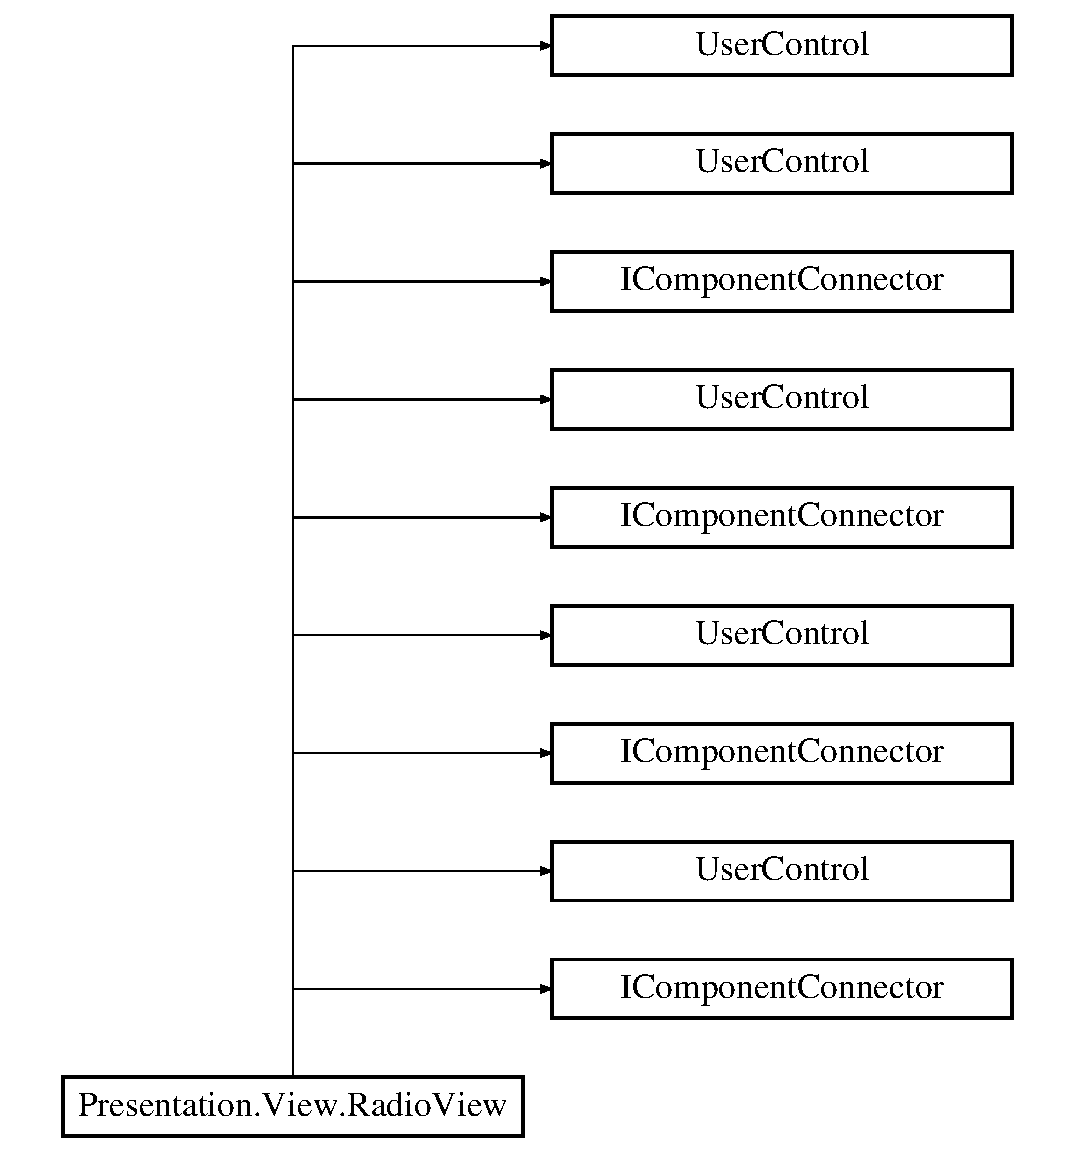
\includegraphics[height=10.000000cm]{class_presentation_1_1_view_1_1_radio_view}
\end{center}
\end{figure}
\subsection*{Public Member Functions}
\begin{DoxyCompactItemize}
\item 
void \hyperlink{class_presentation_1_1_view_1_1_radio_view_a1ecaa37c7376879dae58561a0a3266d8}{Initialize\+Component} ()
\begin{DoxyCompactList}\small\item\em Initialize\+Component \end{DoxyCompactList}\item 
void \hyperlink{class_presentation_1_1_view_1_1_radio_view_a1ecaa37c7376879dae58561a0a3266d8}{Initialize\+Component} ()
\begin{DoxyCompactList}\small\item\em Initialize\+Component \end{DoxyCompactList}\item 
void \hyperlink{class_presentation_1_1_view_1_1_radio_view_a1ecaa37c7376879dae58561a0a3266d8}{Initialize\+Component} ()
\begin{DoxyCompactList}\small\item\em Initialize\+Component \end{DoxyCompactList}\item 
void \hyperlink{class_presentation_1_1_view_1_1_radio_view_a1ecaa37c7376879dae58561a0a3266d8}{Initialize\+Component} ()
\begin{DoxyCompactList}\small\item\em Initialize\+Component \end{DoxyCompactList}\end{DoxyCompactItemize}


\subsection{Detailed Description}
\hyperlink{class_presentation_1_1_view_1_1_radio_view}{Radio\+View} 

Interaction logic for Running.\+xaml 

\subsection{Member Function Documentation}
\mbox{\Hypertarget{class_presentation_1_1_view_1_1_radio_view_a1ecaa37c7376879dae58561a0a3266d8}\label{class_presentation_1_1_view_1_1_radio_view_a1ecaa37c7376879dae58561a0a3266d8}} 
\index{Presentation\+::\+View\+::\+Radio\+View@{Presentation\+::\+View\+::\+Radio\+View}!Initialize\+Component@{Initialize\+Component}}
\index{Initialize\+Component@{Initialize\+Component}!Presentation\+::\+View\+::\+Radio\+View@{Presentation\+::\+View\+::\+Radio\+View}}
\subsubsection{\texorpdfstring{Initialize\+Component()}{InitializeComponent()}\hspace{0.1cm}{\footnotesize\ttfamily [1/4]}}
{\footnotesize\ttfamily void Presentation.\+View.\+Radio\+View.\+Initialize\+Component (\begin{DoxyParamCaption}{ }\end{DoxyParamCaption})}



Initialize\+Component 

\mbox{\Hypertarget{class_presentation_1_1_view_1_1_radio_view_a1ecaa37c7376879dae58561a0a3266d8}\label{class_presentation_1_1_view_1_1_radio_view_a1ecaa37c7376879dae58561a0a3266d8}} 
\index{Presentation\+::\+View\+::\+Radio\+View@{Presentation\+::\+View\+::\+Radio\+View}!Initialize\+Component@{Initialize\+Component}}
\index{Initialize\+Component@{Initialize\+Component}!Presentation\+::\+View\+::\+Radio\+View@{Presentation\+::\+View\+::\+Radio\+View}}
\subsubsection{\texorpdfstring{Initialize\+Component()}{InitializeComponent()}\hspace{0.1cm}{\footnotesize\ttfamily [2/4]}}
{\footnotesize\ttfamily void Presentation.\+View.\+Radio\+View.\+Initialize\+Component (\begin{DoxyParamCaption}{ }\end{DoxyParamCaption})}



Initialize\+Component 

\mbox{\Hypertarget{class_presentation_1_1_view_1_1_radio_view_a1ecaa37c7376879dae58561a0a3266d8}\label{class_presentation_1_1_view_1_1_radio_view_a1ecaa37c7376879dae58561a0a3266d8}} 
\index{Presentation\+::\+View\+::\+Radio\+View@{Presentation\+::\+View\+::\+Radio\+View}!Initialize\+Component@{Initialize\+Component}}
\index{Initialize\+Component@{Initialize\+Component}!Presentation\+::\+View\+::\+Radio\+View@{Presentation\+::\+View\+::\+Radio\+View}}
\subsubsection{\texorpdfstring{Initialize\+Component()}{InitializeComponent()}\hspace{0.1cm}{\footnotesize\ttfamily [3/4]}}
{\footnotesize\ttfamily void Presentation.\+View.\+Radio\+View.\+Initialize\+Component (\begin{DoxyParamCaption}{ }\end{DoxyParamCaption})}



Initialize\+Component 

\mbox{\Hypertarget{class_presentation_1_1_view_1_1_radio_view_a1ecaa37c7376879dae58561a0a3266d8}\label{class_presentation_1_1_view_1_1_radio_view_a1ecaa37c7376879dae58561a0a3266d8}} 
\index{Presentation\+::\+View\+::\+Radio\+View@{Presentation\+::\+View\+::\+Radio\+View}!Initialize\+Component@{Initialize\+Component}}
\index{Initialize\+Component@{Initialize\+Component}!Presentation\+::\+View\+::\+Radio\+View@{Presentation\+::\+View\+::\+Radio\+View}}
\subsubsection{\texorpdfstring{Initialize\+Component()}{InitializeComponent()}\hspace{0.1cm}{\footnotesize\ttfamily [4/4]}}
{\footnotesize\ttfamily void Presentation.\+View.\+Radio\+View.\+Initialize\+Component (\begin{DoxyParamCaption}{ }\end{DoxyParamCaption})}



Initialize\+Component 



The documentation for this class was generated from the following files\+:\begin{DoxyCompactItemize}
\item 
C\+:/\+W\+O\+R\+K\+S\+P\+A\+C\+E/\+T\+P\+I-\/end/\+Gestion\+Audio/\+Gestion\+Audio/obj/\+Debug/\+View/Radio\+View.\+g.\+cs\item 
C\+:/\+W\+O\+R\+K\+S\+P\+A\+C\+E/\+T\+P\+I-\/end/\+Gestion\+Audio/\+Gestion\+Audio/obj/\+Debug/\+View/Radio\+View.\+g.\+i.\+cs\item 
C\+:/\+W\+O\+R\+K\+S\+P\+A\+C\+E/\+T\+P\+I-\/end/\+Gestion\+Audio/\+Gestion\+Audio/\+View/Radio\+View.\+xaml.\+cs\end{DoxyCompactItemize}

\hypertarget{class_presentation_1_1_view_model_1_1_radio_view_model}{}\section{Presentation.\+View\+Model.\+Radio\+View\+Model Class Reference}
\label{class_presentation_1_1_view_model_1_1_radio_view_model}\index{Presentation.\+View\+Model.\+Radio\+View\+Model@{Presentation.\+View\+Model.\+Radio\+View\+Model}}


This class contain the logic for the radioview  


Inheritance diagram for Presentation.\+View\+Model.\+Radio\+View\+Model\+:\begin{figure}[H]
\begin{center}
\leavevmode
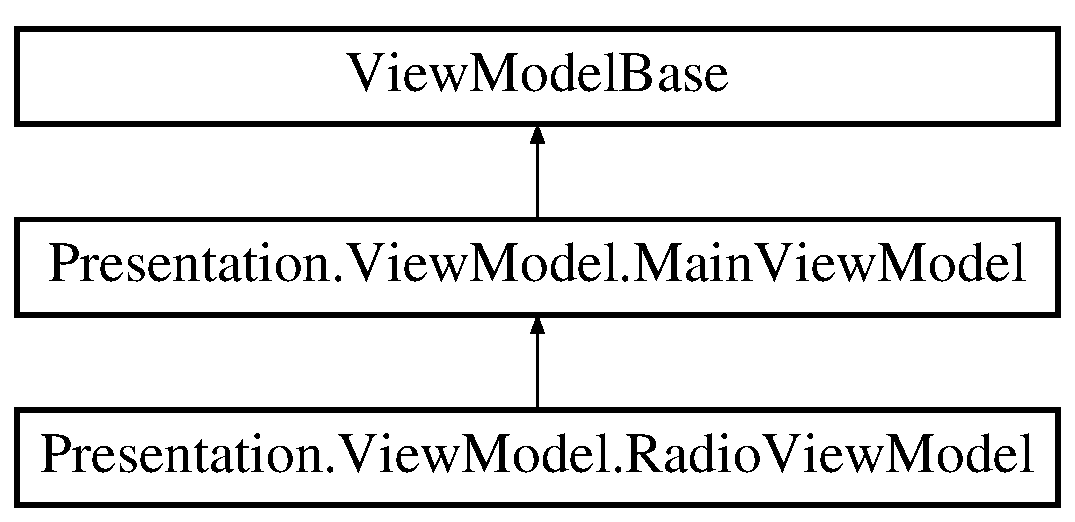
\includegraphics[height=3.000000cm]{class_presentation_1_1_view_model_1_1_radio_view_model}
\end{center}
\end{figure}
\subsection*{Public Member Functions}
\begin{DoxyCompactItemize}
\item 
\hyperlink{class_presentation_1_1_view_model_1_1_radio_view_model_a4aef9d2a4f49274c52d5a6ea6007a5f1}{Radio\+View\+Model} (bool instant\+Load\+Radio=false)
\begin{DoxyCompactList}\small\item\em Set the radio view \end{DoxyCompactList}\item 
\mbox{\Hypertarget{class_presentation_1_1_view_model_1_1_radio_view_model_a0ba2835000d7714bde77a6190ef21938}\label{class_presentation_1_1_view_model_1_1_radio_view_model_a0ba2835000d7714bde77a6190ef21938}} 
{\bfseries Radio\+View\+Model} (List$<$ \hyperlink{class_d_t_o_1_1_entity_1_1_radio}{Radio} $>$ radios)
\item 
async void \hyperlink{class_presentation_1_1_view_model_1_1_radio_view_model_a30f5ad6064bd95c78ecc66061b7e7afb}{Click\+Radio} ()
\begin{DoxyCompactList}\small\item\em When the user click on a radio \end{DoxyCompactList}\item 
void \hyperlink{class_presentation_1_1_view_model_1_1_radio_view_model_a66d0f5118de150b5c1cc6cde2eef710a}{Set\+Favorite} ()
\begin{DoxyCompactList}\small\item\em Set the list of all favorites radios \end{DoxyCompactList}\end{DoxyCompactItemize}
\subsection*{Properties}
\begin{DoxyCompactItemize}
\item 
\mbox{\Hypertarget{class_presentation_1_1_view_model_1_1_radio_view_model_a2ad0f43696a0ee6938f82c3fb82638f4}\label{class_presentation_1_1_view_model_1_1_radio_view_model_a2ad0f43696a0ee6938f82c3fb82638f4}} 
Observable\+Collection$<$ \hyperlink{class_d_t_o_1_1_entity_1_1_radio}{Radio} $>$ {\bfseries Favorites}\hspace{0.3cm}{\ttfamily  \mbox{[}get, set\mbox{]}}
\item 
\mbox{\Hypertarget{class_presentation_1_1_view_model_1_1_radio_view_model_a90346596db447a2c8dfdb631623456bf}\label{class_presentation_1_1_view_model_1_1_radio_view_model_a90346596db447a2c8dfdb631623456bf}} 
Observable\+Collection$<$ \hyperlink{class_d_t_o_1_1_entity_1_1_radio}{Radio} $>$ {\bfseries Last\+Radios} = new Observable\+Collection$<$\hyperlink{class_d_t_o_1_1_entity_1_1_radio}{Radio}$>$()\hspace{0.3cm}{\ttfamily  \mbox{[}get, set\mbox{]}}
\item 
\mbox{\Hypertarget{class_presentation_1_1_view_model_1_1_radio_view_model_a9e2abbd9a4f24623faf92c012446b5ea}\label{class_presentation_1_1_view_model_1_1_radio_view_model_a9e2abbd9a4f24623faf92c012446b5ea}} 
Relay\+Command {\bfseries On\+Click\+Element} = new Observable\+Collection$<$\hyperlink{class_d_t_o_1_1_entity_1_1_radio}{Radio}$>$()\hspace{0.3cm}{\ttfamily  \mbox{[}get, set\mbox{]}}
\item 
\mbox{\Hypertarget{class_presentation_1_1_view_model_1_1_radio_view_model_a3ae8d972e88c7675dfe83fee21f4192f}\label{class_presentation_1_1_view_model_1_1_radio_view_model_a3ae8d972e88c7675dfe83fee21f4192f}} 
Relay\+Command {\bfseries On\+Right\+Click\+Radio}\hspace{0.3cm}{\ttfamily  \mbox{[}get, set\mbox{]}}
\item 
\mbox{\Hypertarget{class_presentation_1_1_view_model_1_1_radio_view_model_af036b68b8628aa922fef14c18be9ede5}\label{class_presentation_1_1_view_model_1_1_radio_view_model_af036b68b8628aa922fef14c18be9ede5}} 
Observable\+Collection$<$ \hyperlink{class_d_t_o_1_1_entity_1_1_radio}{Radio} $>$ {\bfseries Radios}\hspace{0.3cm}{\ttfamily  \mbox{[}get, set\mbox{]}}
\item 
\mbox{\Hypertarget{class_presentation_1_1_view_model_1_1_radio_view_model_ad9487bf37aee2b51ce7cbce807f54071}\label{class_presentation_1_1_view_model_1_1_radio_view_model_ad9487bf37aee2b51ce7cbce807f54071}} 
\hyperlink{class_d_t_o_1_1_entity_1_1_radio}{Radio} {\bfseries Selected\+Item} = new Observable\+Collection$<$\hyperlink{class_d_t_o_1_1_entity_1_1_radio}{Radio}$>$()\hspace{0.3cm}{\ttfamily  \mbox{[}get, set\mbox{]}}
\end{DoxyCompactItemize}


\subsection{Detailed Description}
This class contain the logic for the radioview 



\subsection{Constructor \& Destructor Documentation}
\mbox{\Hypertarget{class_presentation_1_1_view_model_1_1_radio_view_model_a4aef9d2a4f49274c52d5a6ea6007a5f1}\label{class_presentation_1_1_view_model_1_1_radio_view_model_a4aef9d2a4f49274c52d5a6ea6007a5f1}} 
\index{Presentation\+::\+View\+Model\+::\+Radio\+View\+Model@{Presentation\+::\+View\+Model\+::\+Radio\+View\+Model}!Radio\+View\+Model@{Radio\+View\+Model}}
\index{Radio\+View\+Model@{Radio\+View\+Model}!Presentation\+::\+View\+Model\+::\+Radio\+View\+Model@{Presentation\+::\+View\+Model\+::\+Radio\+View\+Model}}
\subsubsection{\texorpdfstring{Radio\+View\+Model()}{RadioViewModel()}}
{\footnotesize\ttfamily Presentation.\+View\+Model.\+Radio\+View\+Model.\+Radio\+View\+Model (\begin{DoxyParamCaption}\item[{bool}]{instant\+Load\+Radio = {\ttfamily false} }\end{DoxyParamCaption})}



Set the radio view 


\begin{DoxyParams}{Parameters}
{\em instant\+Load\+Radio} & \\
\hline
\end{DoxyParams}


\subsection{Member Function Documentation}
\mbox{\Hypertarget{class_presentation_1_1_view_model_1_1_radio_view_model_a30f5ad6064bd95c78ecc66061b7e7afb}\label{class_presentation_1_1_view_model_1_1_radio_view_model_a30f5ad6064bd95c78ecc66061b7e7afb}} 
\index{Presentation\+::\+View\+Model\+::\+Radio\+View\+Model@{Presentation\+::\+View\+Model\+::\+Radio\+View\+Model}!Click\+Radio@{Click\+Radio}}
\index{Click\+Radio@{Click\+Radio}!Presentation\+::\+View\+Model\+::\+Radio\+View\+Model@{Presentation\+::\+View\+Model\+::\+Radio\+View\+Model}}
\subsubsection{\texorpdfstring{Click\+Radio()}{ClickRadio()}}
{\footnotesize\ttfamily async void Presentation.\+View\+Model.\+Radio\+View\+Model.\+Click\+Radio (\begin{DoxyParamCaption}{ }\end{DoxyParamCaption})}



When the user click on a radio 

\mbox{\Hypertarget{class_presentation_1_1_view_model_1_1_radio_view_model_a66d0f5118de150b5c1cc6cde2eef710a}\label{class_presentation_1_1_view_model_1_1_radio_view_model_a66d0f5118de150b5c1cc6cde2eef710a}} 
\index{Presentation\+::\+View\+Model\+::\+Radio\+View\+Model@{Presentation\+::\+View\+Model\+::\+Radio\+View\+Model}!Set\+Favorite@{Set\+Favorite}}
\index{Set\+Favorite@{Set\+Favorite}!Presentation\+::\+View\+Model\+::\+Radio\+View\+Model@{Presentation\+::\+View\+Model\+::\+Radio\+View\+Model}}
\subsubsection{\texorpdfstring{Set\+Favorite()}{SetFavorite()}}
{\footnotesize\ttfamily void Presentation.\+View\+Model.\+Radio\+View\+Model.\+Set\+Favorite (\begin{DoxyParamCaption}{ }\end{DoxyParamCaption})}



Set the list of all favorites radios 



The documentation for this class was generated from the following file\+:\begin{DoxyCompactItemize}
\item 
C\+:/\+W\+O\+R\+K\+S\+P\+A\+C\+E/\+T\+P\+I-\/end/\+Gestion\+Audio/\+Gestion\+Audio/\+View\+Model/Radio\+View\+Model.\+cs\end{DoxyCompactItemize}

\hypertarget{class_presentation_1_1_view_1_1_flyout_1_1_reading_flyout_view}{}\section{Presentation.\+View.\+Flyout.\+Reading\+Flyout\+View Class Reference}
\label{class_presentation_1_1_view_1_1_flyout_1_1_reading_flyout_view}\index{Presentation.\+View.\+Flyout.\+Reading\+Flyout\+View@{Presentation.\+View.\+Flyout.\+Reading\+Flyout\+View}}


\hyperlink{class_presentation_1_1_view_1_1_flyout_1_1_reading_flyout_view}{Reading\+Flyout\+View}  


Inheritance diagram for Presentation.\+View.\+Flyout.\+Reading\+Flyout\+View\+:\begin{figure}[H]
\begin{center}
\leavevmode
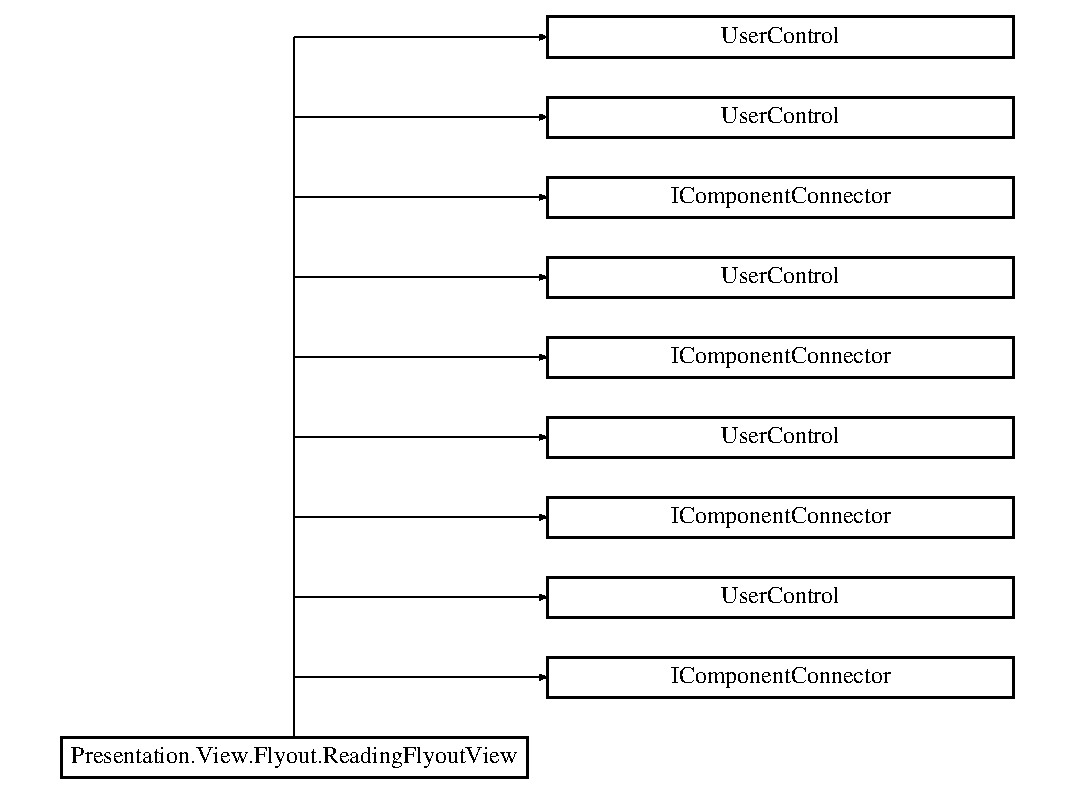
\includegraphics[height=10.000000cm]{class_presentation_1_1_view_1_1_flyout_1_1_reading_flyout_view}
\end{center}
\end{figure}
\subsection*{Public Member Functions}
\begin{DoxyCompactItemize}
\item 
void \hyperlink{class_presentation_1_1_view_1_1_flyout_1_1_reading_flyout_view_a56201647e9af359ad367496f91779872}{Initialize\+Component} ()
\begin{DoxyCompactList}\small\item\em Initialize\+Component \end{DoxyCompactList}\item 
void \hyperlink{class_presentation_1_1_view_1_1_flyout_1_1_reading_flyout_view_a56201647e9af359ad367496f91779872}{Initialize\+Component} ()
\begin{DoxyCompactList}\small\item\em Initialize\+Component \end{DoxyCompactList}\item 
void \hyperlink{class_presentation_1_1_view_1_1_flyout_1_1_reading_flyout_view_a56201647e9af359ad367496f91779872}{Initialize\+Component} ()
\begin{DoxyCompactList}\small\item\em Initialize\+Component \end{DoxyCompactList}\item 
void \hyperlink{class_presentation_1_1_view_1_1_flyout_1_1_reading_flyout_view_a56201647e9af359ad367496f91779872}{Initialize\+Component} ()
\begin{DoxyCompactList}\small\item\em Initialize\+Component \end{DoxyCompactList}\end{DoxyCompactItemize}


\subsection{Detailed Description}
\hyperlink{class_presentation_1_1_view_1_1_flyout_1_1_reading_flyout_view}{Reading\+Flyout\+View} 

Interaction logic for Running\+Flyout\+View.\+xaml 

\subsection{Member Function Documentation}
\mbox{\Hypertarget{class_presentation_1_1_view_1_1_flyout_1_1_reading_flyout_view_a56201647e9af359ad367496f91779872}\label{class_presentation_1_1_view_1_1_flyout_1_1_reading_flyout_view_a56201647e9af359ad367496f91779872}} 
\index{Presentation\+::\+View\+::\+Flyout\+::\+Reading\+Flyout\+View@{Presentation\+::\+View\+::\+Flyout\+::\+Reading\+Flyout\+View}!Initialize\+Component@{Initialize\+Component}}
\index{Initialize\+Component@{Initialize\+Component}!Presentation\+::\+View\+::\+Flyout\+::\+Reading\+Flyout\+View@{Presentation\+::\+View\+::\+Flyout\+::\+Reading\+Flyout\+View}}
\subsubsection{\texorpdfstring{Initialize\+Component()}{InitializeComponent()}\hspace{0.1cm}{\footnotesize\ttfamily [1/4]}}
{\footnotesize\ttfamily void Presentation.\+View.\+Flyout.\+Reading\+Flyout\+View.\+Initialize\+Component (\begin{DoxyParamCaption}{ }\end{DoxyParamCaption})}



Initialize\+Component 

\mbox{\Hypertarget{class_presentation_1_1_view_1_1_flyout_1_1_reading_flyout_view_a56201647e9af359ad367496f91779872}\label{class_presentation_1_1_view_1_1_flyout_1_1_reading_flyout_view_a56201647e9af359ad367496f91779872}} 
\index{Presentation\+::\+View\+::\+Flyout\+::\+Reading\+Flyout\+View@{Presentation\+::\+View\+::\+Flyout\+::\+Reading\+Flyout\+View}!Initialize\+Component@{Initialize\+Component}}
\index{Initialize\+Component@{Initialize\+Component}!Presentation\+::\+View\+::\+Flyout\+::\+Reading\+Flyout\+View@{Presentation\+::\+View\+::\+Flyout\+::\+Reading\+Flyout\+View}}
\subsubsection{\texorpdfstring{Initialize\+Component()}{InitializeComponent()}\hspace{0.1cm}{\footnotesize\ttfamily [2/4]}}
{\footnotesize\ttfamily void Presentation.\+View.\+Flyout.\+Reading\+Flyout\+View.\+Initialize\+Component (\begin{DoxyParamCaption}{ }\end{DoxyParamCaption})}



Initialize\+Component 

\mbox{\Hypertarget{class_presentation_1_1_view_1_1_flyout_1_1_reading_flyout_view_a56201647e9af359ad367496f91779872}\label{class_presentation_1_1_view_1_1_flyout_1_1_reading_flyout_view_a56201647e9af359ad367496f91779872}} 
\index{Presentation\+::\+View\+::\+Flyout\+::\+Reading\+Flyout\+View@{Presentation\+::\+View\+::\+Flyout\+::\+Reading\+Flyout\+View}!Initialize\+Component@{Initialize\+Component}}
\index{Initialize\+Component@{Initialize\+Component}!Presentation\+::\+View\+::\+Flyout\+::\+Reading\+Flyout\+View@{Presentation\+::\+View\+::\+Flyout\+::\+Reading\+Flyout\+View}}
\subsubsection{\texorpdfstring{Initialize\+Component()}{InitializeComponent()}\hspace{0.1cm}{\footnotesize\ttfamily [3/4]}}
{\footnotesize\ttfamily void Presentation.\+View.\+Flyout.\+Reading\+Flyout\+View.\+Initialize\+Component (\begin{DoxyParamCaption}{ }\end{DoxyParamCaption})}



Initialize\+Component 

\mbox{\Hypertarget{class_presentation_1_1_view_1_1_flyout_1_1_reading_flyout_view_a56201647e9af359ad367496f91779872}\label{class_presentation_1_1_view_1_1_flyout_1_1_reading_flyout_view_a56201647e9af359ad367496f91779872}} 
\index{Presentation\+::\+View\+::\+Flyout\+::\+Reading\+Flyout\+View@{Presentation\+::\+View\+::\+Flyout\+::\+Reading\+Flyout\+View}!Initialize\+Component@{Initialize\+Component}}
\index{Initialize\+Component@{Initialize\+Component}!Presentation\+::\+View\+::\+Flyout\+::\+Reading\+Flyout\+View@{Presentation\+::\+View\+::\+Flyout\+::\+Reading\+Flyout\+View}}
\subsubsection{\texorpdfstring{Initialize\+Component()}{InitializeComponent()}\hspace{0.1cm}{\footnotesize\ttfamily [4/4]}}
{\footnotesize\ttfamily void Presentation.\+View.\+Flyout.\+Reading\+Flyout\+View.\+Initialize\+Component (\begin{DoxyParamCaption}{ }\end{DoxyParamCaption})}



Initialize\+Component 



The documentation for this class was generated from the following files\+:\begin{DoxyCompactItemize}
\item 
C\+:/\+W\+O\+R\+K\+S\+P\+A\+C\+E/\+T\+P\+I-\/end/\+Gestion\+Audio/\+Gestion\+Audio/obj/\+Debug/\+View/\+Flyout/Reading\+Flyout\+View.\+g.\+cs\item 
C\+:/\+W\+O\+R\+K\+S\+P\+A\+C\+E/\+T\+P\+I-\/end/\+Gestion\+Audio/\+Gestion\+Audio/obj/\+Debug/\+View/\+Flyout/Reading\+Flyout\+View.\+g.\+i.\+cs\item 
C\+:/\+W\+O\+R\+K\+S\+P\+A\+C\+E/\+T\+P\+I-\/end/\+Gestion\+Audio/\+Gestion\+Audio/\+View/\+Flyout/Reading\+Flyout\+View.\+xaml.\+cs\end{DoxyCompactItemize}

\hypertarget{class_presentation_1_1_view_1_1_list_1_1_reading_list_view}{}\section{Presentation.\+View.\+List.\+Reading\+List\+View Class Reference}
\label{class_presentation_1_1_view_1_1_list_1_1_reading_list_view}\index{Presentation.\+View.\+List.\+Reading\+List\+View@{Presentation.\+View.\+List.\+Reading\+List\+View}}


\hyperlink{class_presentation_1_1_view_1_1_list_1_1_reading_list_view}{Reading\+List\+View}  


Inheritance diagram for Presentation.\+View.\+List.\+Reading\+List\+View\+:\begin{figure}[H]
\begin{center}
\leavevmode
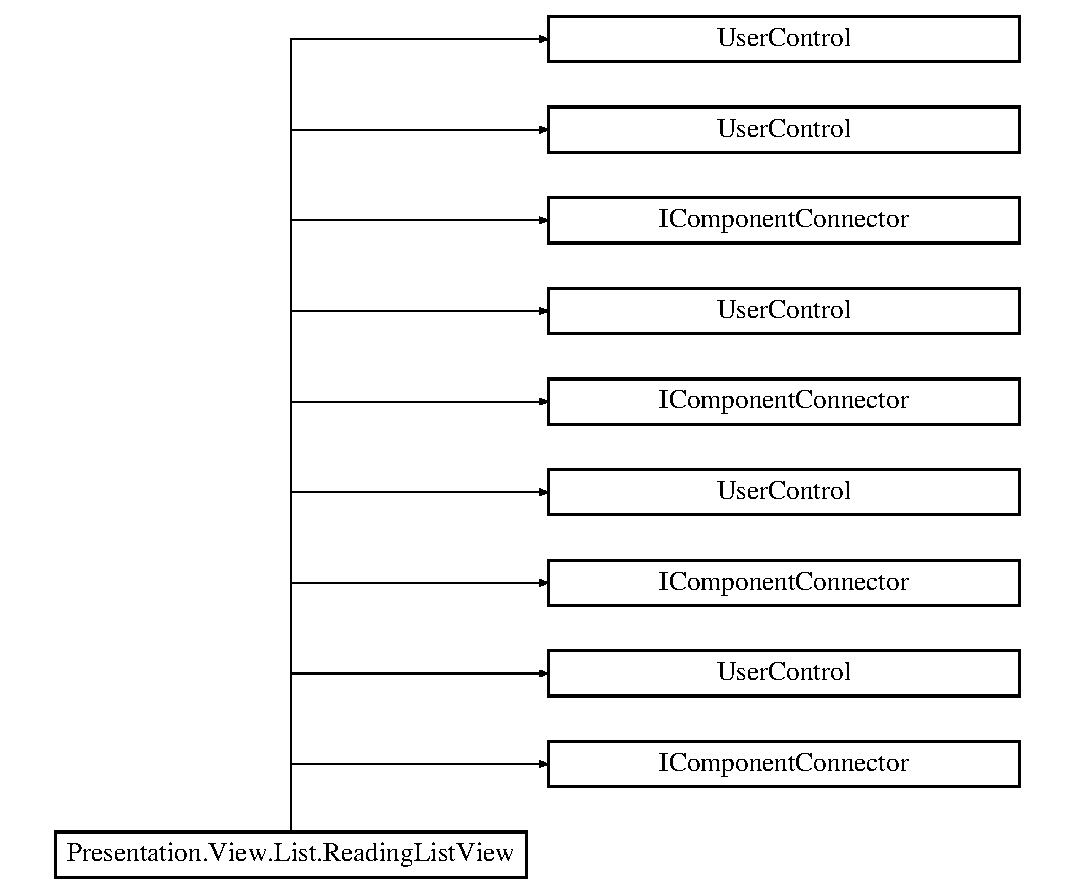
\includegraphics[height=10.000000cm]{class_presentation_1_1_view_1_1_list_1_1_reading_list_view}
\end{center}
\end{figure}
\subsection*{Public Member Functions}
\begin{DoxyCompactItemize}
\item 
void \hyperlink{class_presentation_1_1_view_1_1_list_1_1_reading_list_view_ac889482272d93e01a46d543e008f0e05}{Initialize\+Component} ()
\begin{DoxyCompactList}\small\item\em Initialize\+Component \end{DoxyCompactList}\item 
void \hyperlink{class_presentation_1_1_view_1_1_list_1_1_reading_list_view_ac889482272d93e01a46d543e008f0e05}{Initialize\+Component} ()
\begin{DoxyCompactList}\small\item\em Initialize\+Component \end{DoxyCompactList}\item 
void \hyperlink{class_presentation_1_1_view_1_1_list_1_1_reading_list_view_ac889482272d93e01a46d543e008f0e05}{Initialize\+Component} ()
\begin{DoxyCompactList}\small\item\em Initialize\+Component \end{DoxyCompactList}\item 
void \hyperlink{class_presentation_1_1_view_1_1_list_1_1_reading_list_view_ac889482272d93e01a46d543e008f0e05}{Initialize\+Component} ()
\begin{DoxyCompactList}\small\item\em Initialize\+Component \end{DoxyCompactList}\end{DoxyCompactItemize}


\subsection{Detailed Description}
\hyperlink{class_presentation_1_1_view_1_1_list_1_1_reading_list_view}{Reading\+List\+View} 

Interaction logic for Reading\+List\+View.\+xaml 

\subsection{Member Function Documentation}
\mbox{\Hypertarget{class_presentation_1_1_view_1_1_list_1_1_reading_list_view_ac889482272d93e01a46d543e008f0e05}\label{class_presentation_1_1_view_1_1_list_1_1_reading_list_view_ac889482272d93e01a46d543e008f0e05}} 
\index{Presentation\+::\+View\+::\+List\+::\+Reading\+List\+View@{Presentation\+::\+View\+::\+List\+::\+Reading\+List\+View}!Initialize\+Component@{Initialize\+Component}}
\index{Initialize\+Component@{Initialize\+Component}!Presentation\+::\+View\+::\+List\+::\+Reading\+List\+View@{Presentation\+::\+View\+::\+List\+::\+Reading\+List\+View}}
\subsubsection{\texorpdfstring{Initialize\+Component()}{InitializeComponent()}\hspace{0.1cm}{\footnotesize\ttfamily [1/4]}}
{\footnotesize\ttfamily void Presentation.\+View.\+List.\+Reading\+List\+View.\+Initialize\+Component (\begin{DoxyParamCaption}{ }\end{DoxyParamCaption})}



Initialize\+Component 

\mbox{\Hypertarget{class_presentation_1_1_view_1_1_list_1_1_reading_list_view_ac889482272d93e01a46d543e008f0e05}\label{class_presentation_1_1_view_1_1_list_1_1_reading_list_view_ac889482272d93e01a46d543e008f0e05}} 
\index{Presentation\+::\+View\+::\+List\+::\+Reading\+List\+View@{Presentation\+::\+View\+::\+List\+::\+Reading\+List\+View}!Initialize\+Component@{Initialize\+Component}}
\index{Initialize\+Component@{Initialize\+Component}!Presentation\+::\+View\+::\+List\+::\+Reading\+List\+View@{Presentation\+::\+View\+::\+List\+::\+Reading\+List\+View}}
\subsubsection{\texorpdfstring{Initialize\+Component()}{InitializeComponent()}\hspace{0.1cm}{\footnotesize\ttfamily [2/4]}}
{\footnotesize\ttfamily void Presentation.\+View.\+List.\+Reading\+List\+View.\+Initialize\+Component (\begin{DoxyParamCaption}{ }\end{DoxyParamCaption})}



Initialize\+Component 

\mbox{\Hypertarget{class_presentation_1_1_view_1_1_list_1_1_reading_list_view_ac889482272d93e01a46d543e008f0e05}\label{class_presentation_1_1_view_1_1_list_1_1_reading_list_view_ac889482272d93e01a46d543e008f0e05}} 
\index{Presentation\+::\+View\+::\+List\+::\+Reading\+List\+View@{Presentation\+::\+View\+::\+List\+::\+Reading\+List\+View}!Initialize\+Component@{Initialize\+Component}}
\index{Initialize\+Component@{Initialize\+Component}!Presentation\+::\+View\+::\+List\+::\+Reading\+List\+View@{Presentation\+::\+View\+::\+List\+::\+Reading\+List\+View}}
\subsubsection{\texorpdfstring{Initialize\+Component()}{InitializeComponent()}\hspace{0.1cm}{\footnotesize\ttfamily [3/4]}}
{\footnotesize\ttfamily void Presentation.\+View.\+List.\+Reading\+List\+View.\+Initialize\+Component (\begin{DoxyParamCaption}{ }\end{DoxyParamCaption})}



Initialize\+Component 

\mbox{\Hypertarget{class_presentation_1_1_view_1_1_list_1_1_reading_list_view_ac889482272d93e01a46d543e008f0e05}\label{class_presentation_1_1_view_1_1_list_1_1_reading_list_view_ac889482272d93e01a46d543e008f0e05}} 
\index{Presentation\+::\+View\+::\+List\+::\+Reading\+List\+View@{Presentation\+::\+View\+::\+List\+::\+Reading\+List\+View}!Initialize\+Component@{Initialize\+Component}}
\index{Initialize\+Component@{Initialize\+Component}!Presentation\+::\+View\+::\+List\+::\+Reading\+List\+View@{Presentation\+::\+View\+::\+List\+::\+Reading\+List\+View}}
\subsubsection{\texorpdfstring{Initialize\+Component()}{InitializeComponent()}\hspace{0.1cm}{\footnotesize\ttfamily [4/4]}}
{\footnotesize\ttfamily void Presentation.\+View.\+List.\+Reading\+List\+View.\+Initialize\+Component (\begin{DoxyParamCaption}{ }\end{DoxyParamCaption})}



Initialize\+Component 



The documentation for this class was generated from the following files\+:\begin{DoxyCompactItemize}
\item 
C\+:/\+W\+O\+R\+K\+S\+P\+A\+C\+E/\+T\+P\+I-\/end/\+Gestion\+Audio/\+Gestion\+Audio/obj/\+Debug/\+View/\+List/Reading\+List\+View.\+g.\+cs\item 
C\+:/\+W\+O\+R\+K\+S\+P\+A\+C\+E/\+T\+P\+I-\/end/\+Gestion\+Audio/\+Gestion\+Audio/obj/\+Debug/\+View/\+List/Reading\+List\+View.\+g.\+i.\+cs\item 
C\+:/\+W\+O\+R\+K\+S\+P\+A\+C\+E/\+T\+P\+I-\/end/\+Gestion\+Audio/\+Gestion\+Audio/\+View/\+List/Reading\+List\+View.\+xaml.\+cs\end{DoxyCompactItemize}

\hypertarget{class_presentation_1_1_view_1_1_list_1_1_recent_list_view}{}\section{Presentation.\+View.\+List.\+Recent\+List\+View Class Reference}
\label{class_presentation_1_1_view_1_1_list_1_1_recent_list_view}\index{Presentation.\+View.\+List.\+Recent\+List\+View@{Presentation.\+View.\+List.\+Recent\+List\+View}}


\hyperlink{class_presentation_1_1_view_1_1_list_1_1_recent_list_view}{Recent\+List\+View}  


Inheritance diagram for Presentation.\+View.\+List.\+Recent\+List\+View\+:\begin{figure}[H]
\begin{center}
\leavevmode
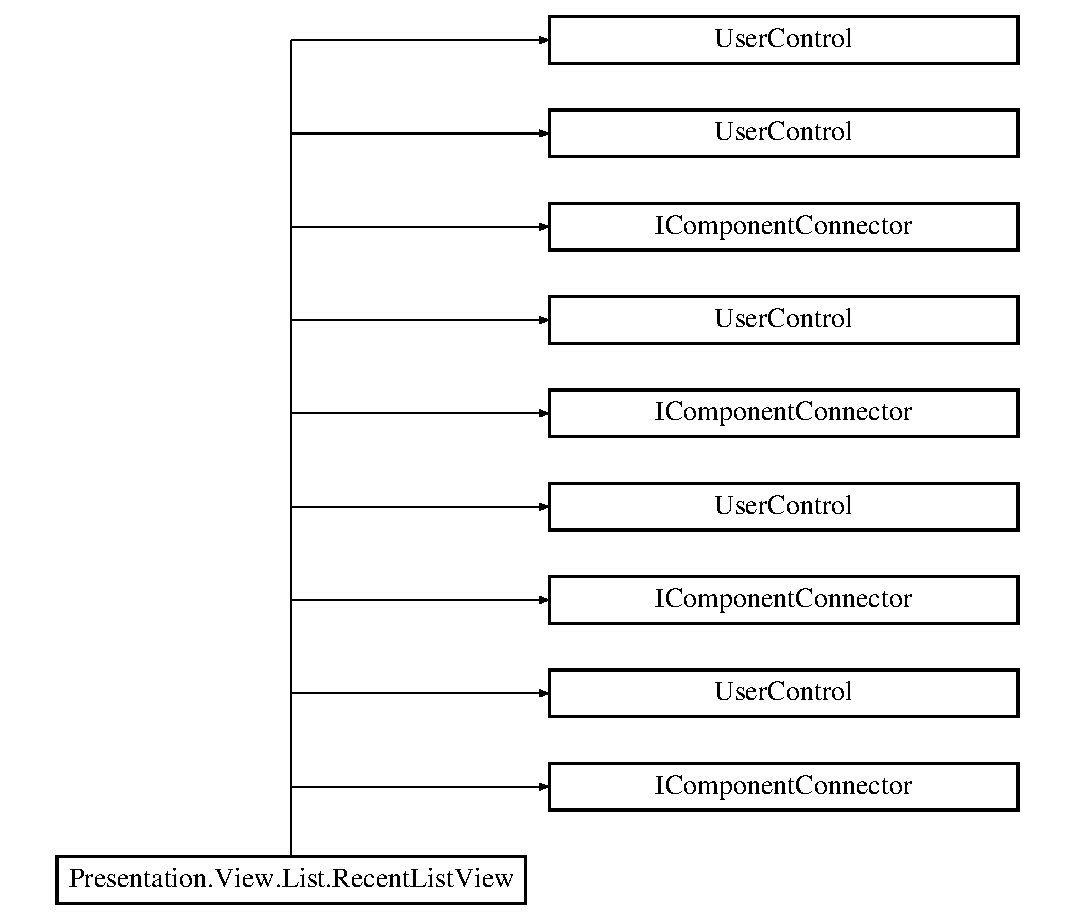
\includegraphics[height=10.000000cm]{class_presentation_1_1_view_1_1_list_1_1_recent_list_view}
\end{center}
\end{figure}
\subsection*{Public Member Functions}
\begin{DoxyCompactItemize}
\item 
void \hyperlink{class_presentation_1_1_view_1_1_list_1_1_recent_list_view_a9b8ba95e34c16c869bd75522ceacb7dc}{Initialize\+Component} ()
\begin{DoxyCompactList}\small\item\em Initialize\+Component \end{DoxyCompactList}\item 
void \hyperlink{class_presentation_1_1_view_1_1_list_1_1_recent_list_view_a9b8ba95e34c16c869bd75522ceacb7dc}{Initialize\+Component} ()
\begin{DoxyCompactList}\small\item\em Initialize\+Component \end{DoxyCompactList}\item 
void \hyperlink{class_presentation_1_1_view_1_1_list_1_1_recent_list_view_a9b8ba95e34c16c869bd75522ceacb7dc}{Initialize\+Component} ()
\begin{DoxyCompactList}\small\item\em Initialize\+Component \end{DoxyCompactList}\item 
void \hyperlink{class_presentation_1_1_view_1_1_list_1_1_recent_list_view_a9b8ba95e34c16c869bd75522ceacb7dc}{Initialize\+Component} ()
\begin{DoxyCompactList}\small\item\em Initialize\+Component \end{DoxyCompactList}\end{DoxyCompactItemize}


\subsection{Detailed Description}
\hyperlink{class_presentation_1_1_view_1_1_list_1_1_recent_list_view}{Recent\+List\+View} 

Interaction logic for Music\+Home.\+xaml 

\subsection{Member Function Documentation}
\mbox{\Hypertarget{class_presentation_1_1_view_1_1_list_1_1_recent_list_view_a9b8ba95e34c16c869bd75522ceacb7dc}\label{class_presentation_1_1_view_1_1_list_1_1_recent_list_view_a9b8ba95e34c16c869bd75522ceacb7dc}} 
\index{Presentation\+::\+View\+::\+List\+::\+Recent\+List\+View@{Presentation\+::\+View\+::\+List\+::\+Recent\+List\+View}!Initialize\+Component@{Initialize\+Component}}
\index{Initialize\+Component@{Initialize\+Component}!Presentation\+::\+View\+::\+List\+::\+Recent\+List\+View@{Presentation\+::\+View\+::\+List\+::\+Recent\+List\+View}}
\subsubsection{\texorpdfstring{Initialize\+Component()}{InitializeComponent()}\hspace{0.1cm}{\footnotesize\ttfamily [1/4]}}
{\footnotesize\ttfamily void Presentation.\+View.\+List.\+Recent\+List\+View.\+Initialize\+Component (\begin{DoxyParamCaption}{ }\end{DoxyParamCaption})}



Initialize\+Component 

\mbox{\Hypertarget{class_presentation_1_1_view_1_1_list_1_1_recent_list_view_a9b8ba95e34c16c869bd75522ceacb7dc}\label{class_presentation_1_1_view_1_1_list_1_1_recent_list_view_a9b8ba95e34c16c869bd75522ceacb7dc}} 
\index{Presentation\+::\+View\+::\+List\+::\+Recent\+List\+View@{Presentation\+::\+View\+::\+List\+::\+Recent\+List\+View}!Initialize\+Component@{Initialize\+Component}}
\index{Initialize\+Component@{Initialize\+Component}!Presentation\+::\+View\+::\+List\+::\+Recent\+List\+View@{Presentation\+::\+View\+::\+List\+::\+Recent\+List\+View}}
\subsubsection{\texorpdfstring{Initialize\+Component()}{InitializeComponent()}\hspace{0.1cm}{\footnotesize\ttfamily [2/4]}}
{\footnotesize\ttfamily void Presentation.\+View.\+List.\+Recent\+List\+View.\+Initialize\+Component (\begin{DoxyParamCaption}{ }\end{DoxyParamCaption})}



Initialize\+Component 

\mbox{\Hypertarget{class_presentation_1_1_view_1_1_list_1_1_recent_list_view_a9b8ba95e34c16c869bd75522ceacb7dc}\label{class_presentation_1_1_view_1_1_list_1_1_recent_list_view_a9b8ba95e34c16c869bd75522ceacb7dc}} 
\index{Presentation\+::\+View\+::\+List\+::\+Recent\+List\+View@{Presentation\+::\+View\+::\+List\+::\+Recent\+List\+View}!Initialize\+Component@{Initialize\+Component}}
\index{Initialize\+Component@{Initialize\+Component}!Presentation\+::\+View\+::\+List\+::\+Recent\+List\+View@{Presentation\+::\+View\+::\+List\+::\+Recent\+List\+View}}
\subsubsection{\texorpdfstring{Initialize\+Component()}{InitializeComponent()}\hspace{0.1cm}{\footnotesize\ttfamily [3/4]}}
{\footnotesize\ttfamily void Presentation.\+View.\+List.\+Recent\+List\+View.\+Initialize\+Component (\begin{DoxyParamCaption}{ }\end{DoxyParamCaption})}



Initialize\+Component 

\mbox{\Hypertarget{class_presentation_1_1_view_1_1_list_1_1_recent_list_view_a9b8ba95e34c16c869bd75522ceacb7dc}\label{class_presentation_1_1_view_1_1_list_1_1_recent_list_view_a9b8ba95e34c16c869bd75522ceacb7dc}} 
\index{Presentation\+::\+View\+::\+List\+::\+Recent\+List\+View@{Presentation\+::\+View\+::\+List\+::\+Recent\+List\+View}!Initialize\+Component@{Initialize\+Component}}
\index{Initialize\+Component@{Initialize\+Component}!Presentation\+::\+View\+::\+List\+::\+Recent\+List\+View@{Presentation\+::\+View\+::\+List\+::\+Recent\+List\+View}}
\subsubsection{\texorpdfstring{Initialize\+Component()}{InitializeComponent()}\hspace{0.1cm}{\footnotesize\ttfamily [4/4]}}
{\footnotesize\ttfamily void Presentation.\+View.\+List.\+Recent\+List\+View.\+Initialize\+Component (\begin{DoxyParamCaption}{ }\end{DoxyParamCaption})}



Initialize\+Component 



The documentation for this class was generated from the following files\+:\begin{DoxyCompactItemize}
\item 
C\+:/\+W\+O\+R\+K\+S\+P\+A\+C\+E/\+T\+P\+I-\/end/\+Gestion\+Audio/\+Gestion\+Audio/obj/\+Debug/\+View/\+List/Recent\+List\+View.\+g.\+cs\item 
C\+:/\+W\+O\+R\+K\+S\+P\+A\+C\+E/\+T\+P\+I-\/end/\+Gestion\+Audio/\+Gestion\+Audio/obj/\+Debug/\+View/\+List/Recent\+List\+View.\+g.\+i.\+cs\item 
C\+:/\+W\+O\+R\+K\+S\+P\+A\+C\+E/\+T\+P\+I-\/end/\+Gestion\+Audio/\+Gestion\+Audio/\+View/\+List/Recent\+List\+View.\+xaml.\+cs\end{DoxyCompactItemize}

\hypertarget{class_d_a_l_1_1_database_1_1_repository}{}\section{D\+A\+L.\+Database.\+Repository$<$ T $>$ Class Template Reference}
\label{class_d_a_l_1_1_database_1_1_repository}\index{D\+A\+L.\+Database.\+Repository$<$ T $>$@{D\+A\+L.\+Database.\+Repository$<$ T $>$}}


Generic class used by all entities, every calls is made on the same context  


\subsection*{Public Member Functions}
\begin{DoxyCompactItemize}
\item 
\hyperlink{class_d_a_l_1_1_database_1_1_repository_a937df992bda81edb925ddc7ffd731f0c}{Repository} ()
\begin{DoxyCompactList}\small\item\em On the first time, create a context \end{DoxyCompactList}\item 
void \hyperlink{class_d_a_l_1_1_database_1_1_repository_a4c49f3a7978384df0e98639b935040b7}{Add\+Or\+Update} (T entity, bool save=true)
\begin{DoxyCompactList}\small\item\em Update or insert an entity \end{DoxyCompactList}\item 
void \hyperlink{class_d_a_l_1_1_database_1_1_repository_a00a8e89402d9f7f7a8035d69b2cf5e31}{Delete} (T entity)
\begin{DoxyCompactList}\small\item\em Delete an entity \end{DoxyCompactList}\item 
T \hyperlink{class_d_a_l_1_1_database_1_1_repository_abee9e993465bcb13da296143fe8b5c3e}{Get\+By\+Id} (object id)
\begin{DoxyCompactList}\small\item\em Get an entity by Id \end{DoxyCompactList}\item 
List$<$ T $>$ \hyperlink{class_d_a_l_1_1_database_1_1_repository_aad0464a6d5b228ea60b3dbb281569e21}{Get\+List} ()
\begin{DoxyCompactList}\small\item\em Get all entity from database \end{DoxyCompactList}\end{DoxyCompactItemize}
\subsection*{Public Attributes}
\begin{DoxyCompactItemize}
\item 
\mbox{\Hypertarget{class_d_a_l_1_1_database_1_1_repository_abb10bb5517401514b62f812635f9fcc1}\label{class_d_a_l_1_1_database_1_1_repository_abb10bb5517401514b62f812635f9fcc1}} 
virtual I\+Queryable$<$ T $>$ {\bfseries Table} =$>$ Entities
\end{DoxyCompactItemize}


\subsection{Detailed Description}
Generic class used by all entities, every calls is made on the same context 


\begin{DoxyTemplParams}{Template Parameters}
{\em T} & \\
\hline
\end{DoxyTemplParams}
\begin{Desc}
\item[Type Constraints]\begin{description}
\item[{\em T} : {\em Base\+Entity}]\end{description}
\end{Desc}


\subsection{Constructor \& Destructor Documentation}
\mbox{\Hypertarget{class_d_a_l_1_1_database_1_1_repository_a937df992bda81edb925ddc7ffd731f0c}\label{class_d_a_l_1_1_database_1_1_repository_a937df992bda81edb925ddc7ffd731f0c}} 
\index{D\+A\+L\+::\+Database\+::\+Repository@{D\+A\+L\+::\+Database\+::\+Repository}!Repository@{Repository}}
\index{Repository@{Repository}!D\+A\+L\+::\+Database\+::\+Repository@{D\+A\+L\+::\+Database\+::\+Repository}}
\subsubsection{\texorpdfstring{Repository()}{Repository()}}
{\footnotesize\ttfamily \hyperlink{class_d_a_l_1_1_database_1_1_repository}{D\+A\+L.\+Database.\+Repository}$<$ T $>$.\hyperlink{class_d_a_l_1_1_database_1_1_repository}{Repository} (\begin{DoxyParamCaption}{ }\end{DoxyParamCaption})}



On the first time, create a context 



\subsection{Member Function Documentation}
\mbox{\Hypertarget{class_d_a_l_1_1_database_1_1_repository_a4c49f3a7978384df0e98639b935040b7}\label{class_d_a_l_1_1_database_1_1_repository_a4c49f3a7978384df0e98639b935040b7}} 
\index{D\+A\+L\+::\+Database\+::\+Repository@{D\+A\+L\+::\+Database\+::\+Repository}!Add\+Or\+Update@{Add\+Or\+Update}}
\index{Add\+Or\+Update@{Add\+Or\+Update}!D\+A\+L\+::\+Database\+::\+Repository@{D\+A\+L\+::\+Database\+::\+Repository}}
\subsubsection{\texorpdfstring{Add\+Or\+Update()}{AddOrUpdate()}}
{\footnotesize\ttfamily void \hyperlink{class_d_a_l_1_1_database_1_1_repository}{D\+A\+L.\+Database.\+Repository}$<$ T $>$.Add\+Or\+Update (\begin{DoxyParamCaption}\item[{T}]{entity,  }\item[{bool}]{save = {\ttfamily true} }\end{DoxyParamCaption})}



Update or insert an entity 


\begin{DoxyParams}{Parameters}
{\em entity} & \\
\hline
{\em save} & \\
\hline
\end{DoxyParams}
\mbox{\Hypertarget{class_d_a_l_1_1_database_1_1_repository_a00a8e89402d9f7f7a8035d69b2cf5e31}\label{class_d_a_l_1_1_database_1_1_repository_a00a8e89402d9f7f7a8035d69b2cf5e31}} 
\index{D\+A\+L\+::\+Database\+::\+Repository@{D\+A\+L\+::\+Database\+::\+Repository}!Delete@{Delete}}
\index{Delete@{Delete}!D\+A\+L\+::\+Database\+::\+Repository@{D\+A\+L\+::\+Database\+::\+Repository}}
\subsubsection{\texorpdfstring{Delete()}{Delete()}}
{\footnotesize\ttfamily void \hyperlink{class_d_a_l_1_1_database_1_1_repository}{D\+A\+L.\+Database.\+Repository}$<$ T $>$.Delete (\begin{DoxyParamCaption}\item[{T}]{entity }\end{DoxyParamCaption})}



Delete an entity 


\begin{DoxyParams}{Parameters}
{\em entity} & \\
\hline
\end{DoxyParams}
\mbox{\Hypertarget{class_d_a_l_1_1_database_1_1_repository_abee9e993465bcb13da296143fe8b5c3e}\label{class_d_a_l_1_1_database_1_1_repository_abee9e993465bcb13da296143fe8b5c3e}} 
\index{D\+A\+L\+::\+Database\+::\+Repository@{D\+A\+L\+::\+Database\+::\+Repository}!Get\+By\+Id@{Get\+By\+Id}}
\index{Get\+By\+Id@{Get\+By\+Id}!D\+A\+L\+::\+Database\+::\+Repository@{D\+A\+L\+::\+Database\+::\+Repository}}
\subsubsection{\texorpdfstring{Get\+By\+Id()}{GetById()}}
{\footnotesize\ttfamily T \hyperlink{class_d_a_l_1_1_database_1_1_repository}{D\+A\+L.\+Database.\+Repository}$<$ T $>$.Get\+By\+Id (\begin{DoxyParamCaption}\item[{object}]{id }\end{DoxyParamCaption})}



Get an entity by Id 


\begin{DoxyParams}{Parameters}
{\em entity} & \\
\hline
\end{DoxyParams}
\mbox{\Hypertarget{class_d_a_l_1_1_database_1_1_repository_aad0464a6d5b228ea60b3dbb281569e21}\label{class_d_a_l_1_1_database_1_1_repository_aad0464a6d5b228ea60b3dbb281569e21}} 
\index{D\+A\+L\+::\+Database\+::\+Repository@{D\+A\+L\+::\+Database\+::\+Repository}!Get\+List@{Get\+List}}
\index{Get\+List@{Get\+List}!D\+A\+L\+::\+Database\+::\+Repository@{D\+A\+L\+::\+Database\+::\+Repository}}
\subsubsection{\texorpdfstring{Get\+List()}{GetList()}}
{\footnotesize\ttfamily List$<$T$>$ \hyperlink{class_d_a_l_1_1_database_1_1_repository}{D\+A\+L.\+Database.\+Repository}$<$ T $>$.Get\+List (\begin{DoxyParamCaption}{ }\end{DoxyParamCaption})}



Get all entity from database 

\begin{DoxyReturn}{Returns}

\end{DoxyReturn}


The documentation for this class was generated from the following file\+:\begin{DoxyCompactItemize}
\item 
C\+:/\+W\+O\+R\+K\+S\+P\+A\+C\+E/\+T\+P\+I-\/end/\+Gestion\+Audio/\+D\+A\+L/\+Database/Repository.\+cs\end{DoxyCompactItemize}

\hypertarget{class_presentation_1_1_view_1_1_flyout_1_1_running_flyout_view}{}\section{Presentation.\+View.\+Flyout.\+Running\+Flyout\+View Class Reference}
\label{class_presentation_1_1_view_1_1_flyout_1_1_running_flyout_view}\index{Presentation.\+View.\+Flyout.\+Running\+Flyout\+View@{Presentation.\+View.\+Flyout.\+Running\+Flyout\+View}}


\hyperlink{class_presentation_1_1_view_1_1_flyout_1_1_running_flyout_view}{Running\+Flyout\+View}  


Inheritance diagram for Presentation.\+View.\+Flyout.\+Running\+Flyout\+View\+:\begin{figure}[H]
\begin{center}
\leavevmode
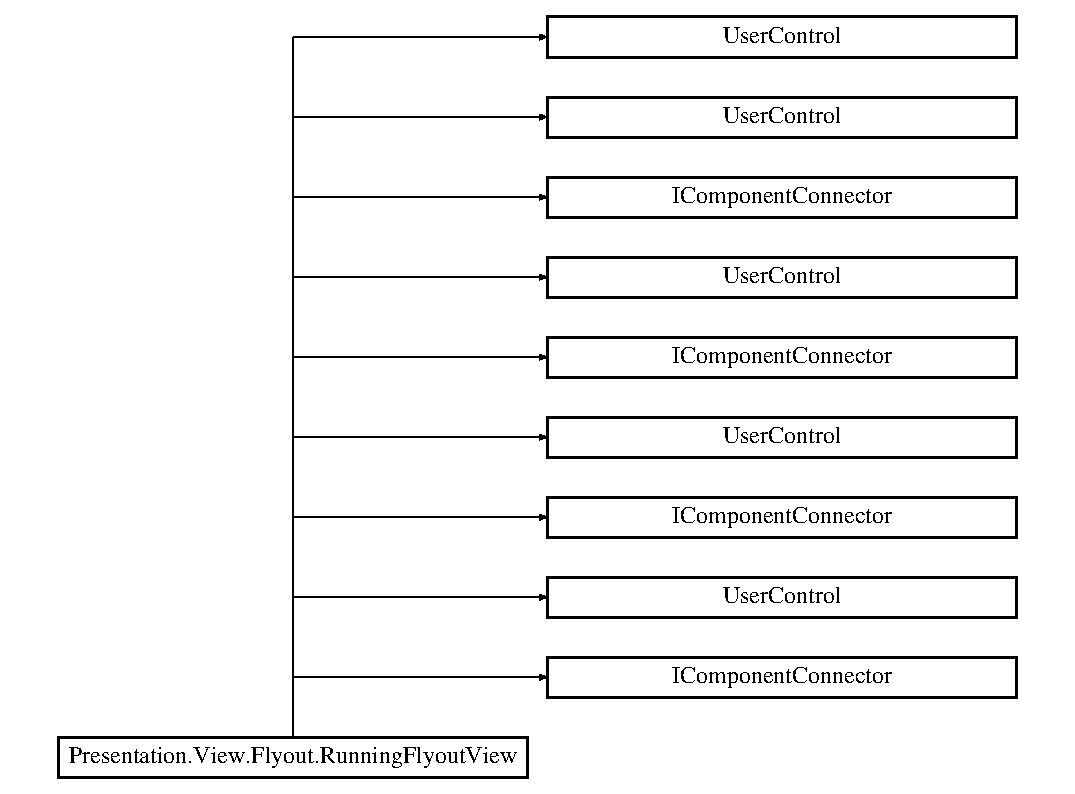
\includegraphics[height=10.000000cm]{class_presentation_1_1_view_1_1_flyout_1_1_running_flyout_view}
\end{center}
\end{figure}
\subsection*{Public Member Functions}
\begin{DoxyCompactItemize}
\item 
void \hyperlink{class_presentation_1_1_view_1_1_flyout_1_1_running_flyout_view_ac284f494bfae1a9a5f8a569710511379}{Initialize\+Component} ()
\begin{DoxyCompactList}\small\item\em Initialize\+Component \end{DoxyCompactList}\item 
void \hyperlink{class_presentation_1_1_view_1_1_flyout_1_1_running_flyout_view_ac284f494bfae1a9a5f8a569710511379}{Initialize\+Component} ()
\begin{DoxyCompactList}\small\item\em Initialize\+Component \end{DoxyCompactList}\item 
void \hyperlink{class_presentation_1_1_view_1_1_flyout_1_1_running_flyout_view_ac284f494bfae1a9a5f8a569710511379}{Initialize\+Component} ()
\begin{DoxyCompactList}\small\item\em Initialize\+Component \end{DoxyCompactList}\item 
void \hyperlink{class_presentation_1_1_view_1_1_flyout_1_1_running_flyout_view_ac284f494bfae1a9a5f8a569710511379}{Initialize\+Component} ()
\begin{DoxyCompactList}\small\item\em Initialize\+Component \end{DoxyCompactList}\end{DoxyCompactItemize}


\subsection{Detailed Description}
\hyperlink{class_presentation_1_1_view_1_1_flyout_1_1_running_flyout_view}{Running\+Flyout\+View} 

Interaction logic for Player\+View.\+xaml 

\subsection{Member Function Documentation}
\mbox{\Hypertarget{class_presentation_1_1_view_1_1_flyout_1_1_running_flyout_view_ac284f494bfae1a9a5f8a569710511379}\label{class_presentation_1_1_view_1_1_flyout_1_1_running_flyout_view_ac284f494bfae1a9a5f8a569710511379}} 
\index{Presentation\+::\+View\+::\+Flyout\+::\+Running\+Flyout\+View@{Presentation\+::\+View\+::\+Flyout\+::\+Running\+Flyout\+View}!Initialize\+Component@{Initialize\+Component}}
\index{Initialize\+Component@{Initialize\+Component}!Presentation\+::\+View\+::\+Flyout\+::\+Running\+Flyout\+View@{Presentation\+::\+View\+::\+Flyout\+::\+Running\+Flyout\+View}}
\subsubsection{\texorpdfstring{Initialize\+Component()}{InitializeComponent()}\hspace{0.1cm}{\footnotesize\ttfamily [1/4]}}
{\footnotesize\ttfamily void Presentation.\+View.\+Flyout.\+Running\+Flyout\+View.\+Initialize\+Component (\begin{DoxyParamCaption}{ }\end{DoxyParamCaption})}



Initialize\+Component 

\mbox{\Hypertarget{class_presentation_1_1_view_1_1_flyout_1_1_running_flyout_view_ac284f494bfae1a9a5f8a569710511379}\label{class_presentation_1_1_view_1_1_flyout_1_1_running_flyout_view_ac284f494bfae1a9a5f8a569710511379}} 
\index{Presentation\+::\+View\+::\+Flyout\+::\+Running\+Flyout\+View@{Presentation\+::\+View\+::\+Flyout\+::\+Running\+Flyout\+View}!Initialize\+Component@{Initialize\+Component}}
\index{Initialize\+Component@{Initialize\+Component}!Presentation\+::\+View\+::\+Flyout\+::\+Running\+Flyout\+View@{Presentation\+::\+View\+::\+Flyout\+::\+Running\+Flyout\+View}}
\subsubsection{\texorpdfstring{Initialize\+Component()}{InitializeComponent()}\hspace{0.1cm}{\footnotesize\ttfamily [2/4]}}
{\footnotesize\ttfamily void Presentation.\+View.\+Flyout.\+Running\+Flyout\+View.\+Initialize\+Component (\begin{DoxyParamCaption}{ }\end{DoxyParamCaption})}



Initialize\+Component 

\mbox{\Hypertarget{class_presentation_1_1_view_1_1_flyout_1_1_running_flyout_view_ac284f494bfae1a9a5f8a569710511379}\label{class_presentation_1_1_view_1_1_flyout_1_1_running_flyout_view_ac284f494bfae1a9a5f8a569710511379}} 
\index{Presentation\+::\+View\+::\+Flyout\+::\+Running\+Flyout\+View@{Presentation\+::\+View\+::\+Flyout\+::\+Running\+Flyout\+View}!Initialize\+Component@{Initialize\+Component}}
\index{Initialize\+Component@{Initialize\+Component}!Presentation\+::\+View\+::\+Flyout\+::\+Running\+Flyout\+View@{Presentation\+::\+View\+::\+Flyout\+::\+Running\+Flyout\+View}}
\subsubsection{\texorpdfstring{Initialize\+Component()}{InitializeComponent()}\hspace{0.1cm}{\footnotesize\ttfamily [3/4]}}
{\footnotesize\ttfamily void Presentation.\+View.\+Flyout.\+Running\+Flyout\+View.\+Initialize\+Component (\begin{DoxyParamCaption}{ }\end{DoxyParamCaption})}



Initialize\+Component 

\mbox{\Hypertarget{class_presentation_1_1_view_1_1_flyout_1_1_running_flyout_view_ac284f494bfae1a9a5f8a569710511379}\label{class_presentation_1_1_view_1_1_flyout_1_1_running_flyout_view_ac284f494bfae1a9a5f8a569710511379}} 
\index{Presentation\+::\+View\+::\+Flyout\+::\+Running\+Flyout\+View@{Presentation\+::\+View\+::\+Flyout\+::\+Running\+Flyout\+View}!Initialize\+Component@{Initialize\+Component}}
\index{Initialize\+Component@{Initialize\+Component}!Presentation\+::\+View\+::\+Flyout\+::\+Running\+Flyout\+View@{Presentation\+::\+View\+::\+Flyout\+::\+Running\+Flyout\+View}}
\subsubsection{\texorpdfstring{Initialize\+Component()}{InitializeComponent()}\hspace{0.1cm}{\footnotesize\ttfamily [4/4]}}
{\footnotesize\ttfamily void Presentation.\+View.\+Flyout.\+Running\+Flyout\+View.\+Initialize\+Component (\begin{DoxyParamCaption}{ }\end{DoxyParamCaption})}



Initialize\+Component 



The documentation for this class was generated from the following files\+:\begin{DoxyCompactItemize}
\item 
C\+:/\+W\+O\+R\+K\+S\+P\+A\+C\+E/\+T\+P\+I-\/end/\+Gestion\+Audio/\+Gestion\+Audio/obj/\+Debug/\+View/\+Flyout/Running\+Flyout\+View.\+g.\+cs\item 
C\+:/\+W\+O\+R\+K\+S\+P\+A\+C\+E/\+T\+P\+I-\/end/\+Gestion\+Audio/\+Gestion\+Audio/obj/\+Debug/\+View/\+Flyout/Running\+Flyout\+View.\+g.\+i.\+cs\item 
C\+:/\+W\+O\+R\+K\+S\+P\+A\+C\+E/\+T\+P\+I-\/end/\+Gestion\+Audio/\+Gestion\+Audio/\+View/\+Flyout/Running\+Flyout\+View.\+xaml.\+cs\end{DoxyCompactItemize}

\hypertarget{class_presentation_1_1_view_1_1_search_view}{}\section{Presentation.\+View.\+Search\+View Class Reference}
\label{class_presentation_1_1_view_1_1_search_view}\index{Presentation.\+View.\+Search\+View@{Presentation.\+View.\+Search\+View}}


\hyperlink{class_presentation_1_1_view_1_1_search_view}{Search\+View}  


Inheritance diagram for Presentation.\+View.\+Search\+View\+:\begin{figure}[H]
\begin{center}
\leavevmode
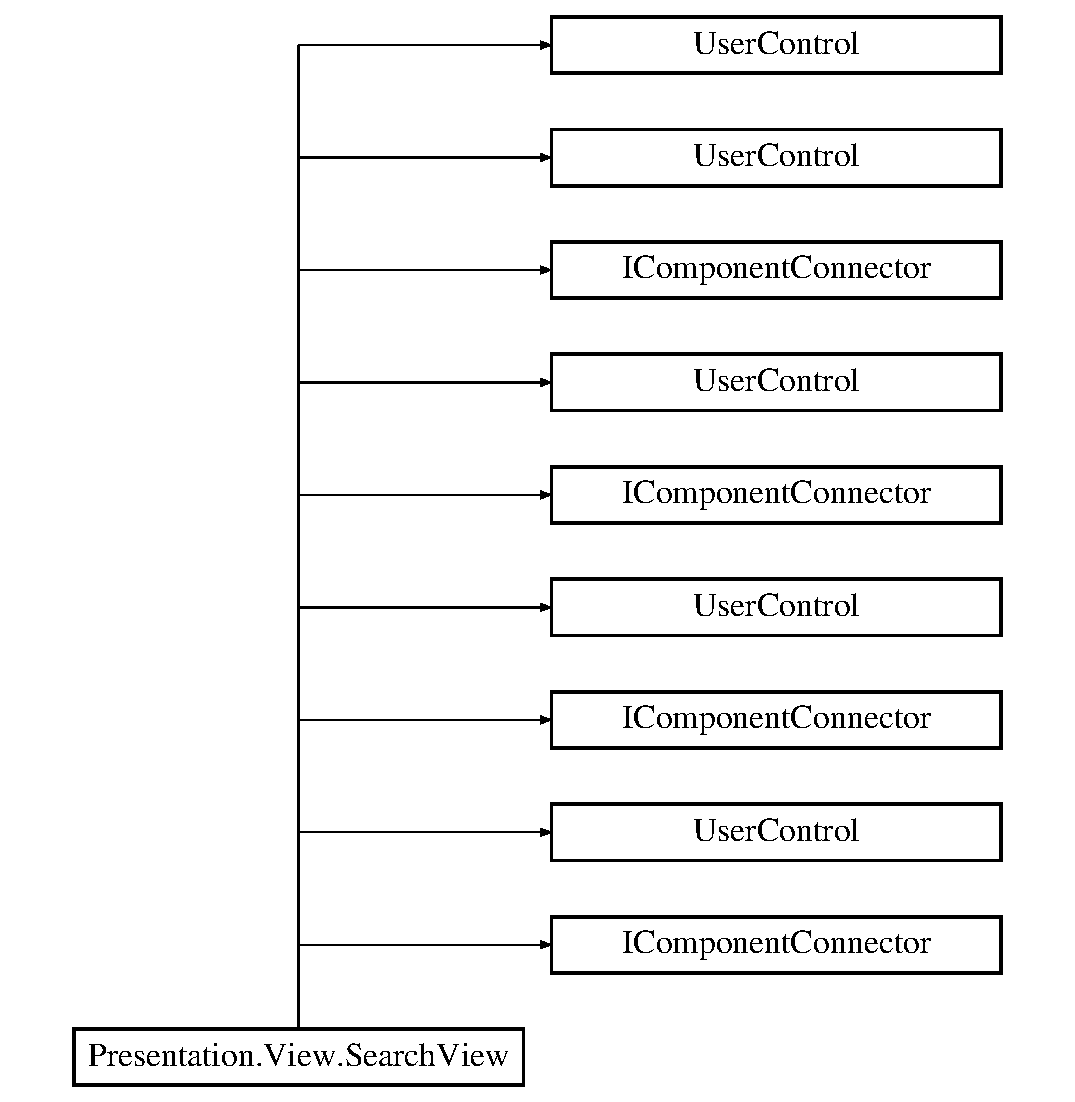
\includegraphics[height=10.000000cm]{class_presentation_1_1_view_1_1_search_view}
\end{center}
\end{figure}
\subsection*{Public Member Functions}
\begin{DoxyCompactItemize}
\item 
void \hyperlink{class_presentation_1_1_view_1_1_search_view_ac553fc7552d2de3e43a6b574d7176220}{Initialize\+Component} ()
\begin{DoxyCompactList}\small\item\em Initialize\+Component \end{DoxyCompactList}\item 
void \hyperlink{class_presentation_1_1_view_1_1_search_view_ac553fc7552d2de3e43a6b574d7176220}{Initialize\+Component} ()
\begin{DoxyCompactList}\small\item\em Initialize\+Component \end{DoxyCompactList}\item 
void \hyperlink{class_presentation_1_1_view_1_1_search_view_ac553fc7552d2de3e43a6b574d7176220}{Initialize\+Component} ()
\begin{DoxyCompactList}\small\item\em Initialize\+Component \end{DoxyCompactList}\item 
void \hyperlink{class_presentation_1_1_view_1_1_search_view_ac553fc7552d2de3e43a6b574d7176220}{Initialize\+Component} ()
\begin{DoxyCompactList}\small\item\em Initialize\+Component \end{DoxyCompactList}\end{DoxyCompactItemize}


\subsection{Detailed Description}
\hyperlink{class_presentation_1_1_view_1_1_search_view}{Search\+View} 

Interaction logic for Running.\+xaml 

\subsection{Member Function Documentation}
\mbox{\Hypertarget{class_presentation_1_1_view_1_1_search_view_ac553fc7552d2de3e43a6b574d7176220}\label{class_presentation_1_1_view_1_1_search_view_ac553fc7552d2de3e43a6b574d7176220}} 
\index{Presentation\+::\+View\+::\+Search\+View@{Presentation\+::\+View\+::\+Search\+View}!Initialize\+Component@{Initialize\+Component}}
\index{Initialize\+Component@{Initialize\+Component}!Presentation\+::\+View\+::\+Search\+View@{Presentation\+::\+View\+::\+Search\+View}}
\subsubsection{\texorpdfstring{Initialize\+Component()}{InitializeComponent()}\hspace{0.1cm}{\footnotesize\ttfamily [1/4]}}
{\footnotesize\ttfamily void Presentation.\+View.\+Search\+View.\+Initialize\+Component (\begin{DoxyParamCaption}{ }\end{DoxyParamCaption})}



Initialize\+Component 

\mbox{\Hypertarget{class_presentation_1_1_view_1_1_search_view_ac553fc7552d2de3e43a6b574d7176220}\label{class_presentation_1_1_view_1_1_search_view_ac553fc7552d2de3e43a6b574d7176220}} 
\index{Presentation\+::\+View\+::\+Search\+View@{Presentation\+::\+View\+::\+Search\+View}!Initialize\+Component@{Initialize\+Component}}
\index{Initialize\+Component@{Initialize\+Component}!Presentation\+::\+View\+::\+Search\+View@{Presentation\+::\+View\+::\+Search\+View}}
\subsubsection{\texorpdfstring{Initialize\+Component()}{InitializeComponent()}\hspace{0.1cm}{\footnotesize\ttfamily [2/4]}}
{\footnotesize\ttfamily void Presentation.\+View.\+Search\+View.\+Initialize\+Component (\begin{DoxyParamCaption}{ }\end{DoxyParamCaption})}



Initialize\+Component 

\mbox{\Hypertarget{class_presentation_1_1_view_1_1_search_view_ac553fc7552d2de3e43a6b574d7176220}\label{class_presentation_1_1_view_1_1_search_view_ac553fc7552d2de3e43a6b574d7176220}} 
\index{Presentation\+::\+View\+::\+Search\+View@{Presentation\+::\+View\+::\+Search\+View}!Initialize\+Component@{Initialize\+Component}}
\index{Initialize\+Component@{Initialize\+Component}!Presentation\+::\+View\+::\+Search\+View@{Presentation\+::\+View\+::\+Search\+View}}
\subsubsection{\texorpdfstring{Initialize\+Component()}{InitializeComponent()}\hspace{0.1cm}{\footnotesize\ttfamily [3/4]}}
{\footnotesize\ttfamily void Presentation.\+View.\+Search\+View.\+Initialize\+Component (\begin{DoxyParamCaption}{ }\end{DoxyParamCaption})}



Initialize\+Component 

\mbox{\Hypertarget{class_presentation_1_1_view_1_1_search_view_ac553fc7552d2de3e43a6b574d7176220}\label{class_presentation_1_1_view_1_1_search_view_ac553fc7552d2de3e43a6b574d7176220}} 
\index{Presentation\+::\+View\+::\+Search\+View@{Presentation\+::\+View\+::\+Search\+View}!Initialize\+Component@{Initialize\+Component}}
\index{Initialize\+Component@{Initialize\+Component}!Presentation\+::\+View\+::\+Search\+View@{Presentation\+::\+View\+::\+Search\+View}}
\subsubsection{\texorpdfstring{Initialize\+Component()}{InitializeComponent()}\hspace{0.1cm}{\footnotesize\ttfamily [4/4]}}
{\footnotesize\ttfamily void Presentation.\+View.\+Search\+View.\+Initialize\+Component (\begin{DoxyParamCaption}{ }\end{DoxyParamCaption})}



Initialize\+Component 



The documentation for this class was generated from the following files\+:\begin{DoxyCompactItemize}
\item 
C\+:/\+W\+O\+R\+K\+S\+P\+A\+C\+E/\+T\+P\+I-\/end/\+Gestion\+Audio/\+Gestion\+Audio/obj/\+Debug/\+View/Search\+View.\+g.\+cs\item 
C\+:/\+W\+O\+R\+K\+S\+P\+A\+C\+E/\+T\+P\+I-\/end/\+Gestion\+Audio/\+Gestion\+Audio/obj/\+Debug/\+View/Search\+View.\+g.\+i.\+cs\item 
C\+:/\+W\+O\+R\+K\+S\+P\+A\+C\+E/\+T\+P\+I-\/end/\+Gestion\+Audio/\+Gestion\+Audio/\+View/Search\+View.\+xaml.\+cs\end{DoxyCompactItemize}

\hypertarget{class_presentation_1_1_view_model_1_1_search_view_model}{}\section{Presentation.\+View\+Model.\+Search\+View\+Model Class Reference}
\label{class_presentation_1_1_view_model_1_1_search_view_model}\index{Presentation.\+View\+Model.\+Search\+View\+Model@{Presentation.\+View\+Model.\+Search\+View\+Model}}


This class contain the logic for the searchview  


Inheritance diagram for Presentation.\+View\+Model.\+Search\+View\+Model\+:\begin{figure}[H]
\begin{center}
\leavevmode
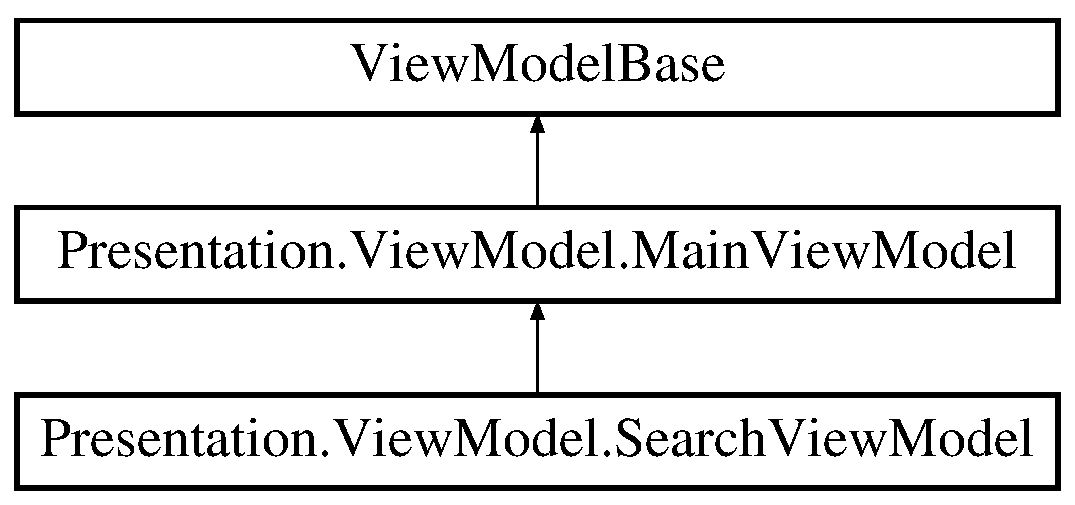
\includegraphics[height=3.000000cm]{class_presentation_1_1_view_model_1_1_search_view_model}
\end{center}
\end{figure}
\subsection*{Public Member Functions}
\begin{DoxyCompactItemize}
\item 
\hyperlink{class_presentation_1_1_view_model_1_1_search_view_model_a325a16f61ed7bc7dedd583b5f5f5faec}{Search\+View\+Model} (string text)
\begin{DoxyCompactList}\small\item\em Launch the search in radios and tracks \end{DoxyCompactList}\end{DoxyCompactItemize}
\subsection*{Static Public Member Functions}
\begin{DoxyCompactItemize}
\item 
static void \hyperlink{class_presentation_1_1_view_model_1_1_search_view_model_aca916aa79980de7c81ac70a9f19ed0e3}{Empty\+Buffer} ()
\begin{DoxyCompactList}\small\item\em empty all buffer list (fired after the sync) \end{DoxyCompactList}\end{DoxyCompactItemize}
\subsection*{Properties}
\begin{DoxyCompactItemize}
\item 
\mbox{\Hypertarget{class_presentation_1_1_view_model_1_1_search_view_model_a8ded5aefcb69f87edbd81318b4018a44}\label{class_presentation_1_1_view_model_1_1_search_view_model_a8ded5aefcb69f87edbd81318b4018a44}} 
string {\bfseries Key\+Word}\hspace{0.3cm}{\ttfamily  \mbox{[}get, set\mbox{]}}
\item 
\mbox{\Hypertarget{class_presentation_1_1_view_model_1_1_search_view_model_affc0751a1fcce107235fbf29e5c91f61}\label{class_presentation_1_1_view_model_1_1_search_view_model_affc0751a1fcce107235fbf29e5c91f61}} 
\hyperlink{class_presentation_1_1_view_model_1_1_music_view_model}{Music\+View\+Model} {\bfseries Music\+View\+Model}\hspace{0.3cm}{\ttfamily  \mbox{[}get, set\mbox{]}}
\item 
\mbox{\Hypertarget{class_presentation_1_1_view_model_1_1_search_view_model_a88c0d8f4fc9d869857814bbad0edd3d2}\label{class_presentation_1_1_view_model_1_1_search_view_model_a88c0d8f4fc9d869857814bbad0edd3d2}} 
\hyperlink{class_presentation_1_1_view_model_1_1_radio_view_model}{Radio\+View\+Model} {\bfseries Radio\+View\+Model}\hspace{0.3cm}{\ttfamily  \mbox{[}get, set\mbox{]}}
\end{DoxyCompactItemize}


\subsection{Detailed Description}
This class contain the logic for the searchview 



\subsection{Constructor \& Destructor Documentation}
\mbox{\Hypertarget{class_presentation_1_1_view_model_1_1_search_view_model_a325a16f61ed7bc7dedd583b5f5f5faec}\label{class_presentation_1_1_view_model_1_1_search_view_model_a325a16f61ed7bc7dedd583b5f5f5faec}} 
\index{Presentation\+::\+View\+Model\+::\+Search\+View\+Model@{Presentation\+::\+View\+Model\+::\+Search\+View\+Model}!Search\+View\+Model@{Search\+View\+Model}}
\index{Search\+View\+Model@{Search\+View\+Model}!Presentation\+::\+View\+Model\+::\+Search\+View\+Model@{Presentation\+::\+View\+Model\+::\+Search\+View\+Model}}
\subsubsection{\texorpdfstring{Search\+View\+Model()}{SearchViewModel()}}
{\footnotesize\ttfamily Presentation.\+View\+Model.\+Search\+View\+Model.\+Search\+View\+Model (\begin{DoxyParamCaption}\item[{string}]{text }\end{DoxyParamCaption})}



Launch the search in radios and tracks 


\begin{DoxyParams}{Parameters}
{\em text} & \\
\hline
\end{DoxyParams}


\subsection{Member Function Documentation}
\mbox{\Hypertarget{class_presentation_1_1_view_model_1_1_search_view_model_aca916aa79980de7c81ac70a9f19ed0e3}\label{class_presentation_1_1_view_model_1_1_search_view_model_aca916aa79980de7c81ac70a9f19ed0e3}} 
\index{Presentation\+::\+View\+Model\+::\+Search\+View\+Model@{Presentation\+::\+View\+Model\+::\+Search\+View\+Model}!Empty\+Buffer@{Empty\+Buffer}}
\index{Empty\+Buffer@{Empty\+Buffer}!Presentation\+::\+View\+Model\+::\+Search\+View\+Model@{Presentation\+::\+View\+Model\+::\+Search\+View\+Model}}
\subsubsection{\texorpdfstring{Empty\+Buffer()}{EmptyBuffer()}}
{\footnotesize\ttfamily static void Presentation.\+View\+Model.\+Search\+View\+Model.\+Empty\+Buffer (\begin{DoxyParamCaption}{ }\end{DoxyParamCaption})\hspace{0.3cm}{\ttfamily [static]}}



empty all buffer list (fired after the sync) 



The documentation for this class was generated from the following file\+:\begin{DoxyCompactItemize}
\item 
C\+:/\+W\+O\+R\+K\+S\+P\+A\+C\+E/\+T\+P\+I-\/end/\+Gestion\+Audio/\+Gestion\+Audio/\+View\+Model/Search\+View\+Model.\+cs\end{DoxyCompactItemize}

\hypertarget{class_presentation_1_1_view_1_1_flyout_1_1_setting_flyout_view}{}\section{Presentation.\+View.\+Flyout.\+Setting\+Flyout\+View Class Reference}
\label{class_presentation_1_1_view_1_1_flyout_1_1_setting_flyout_view}\index{Presentation.\+View.\+Flyout.\+Setting\+Flyout\+View@{Presentation.\+View.\+Flyout.\+Setting\+Flyout\+View}}


\hyperlink{class_presentation_1_1_view_1_1_flyout_1_1_setting_flyout_view}{Setting\+Flyout\+View}  


Inheritance diagram for Presentation.\+View.\+Flyout.\+Setting\+Flyout\+View\+:\begin{figure}[H]
\begin{center}
\leavevmode
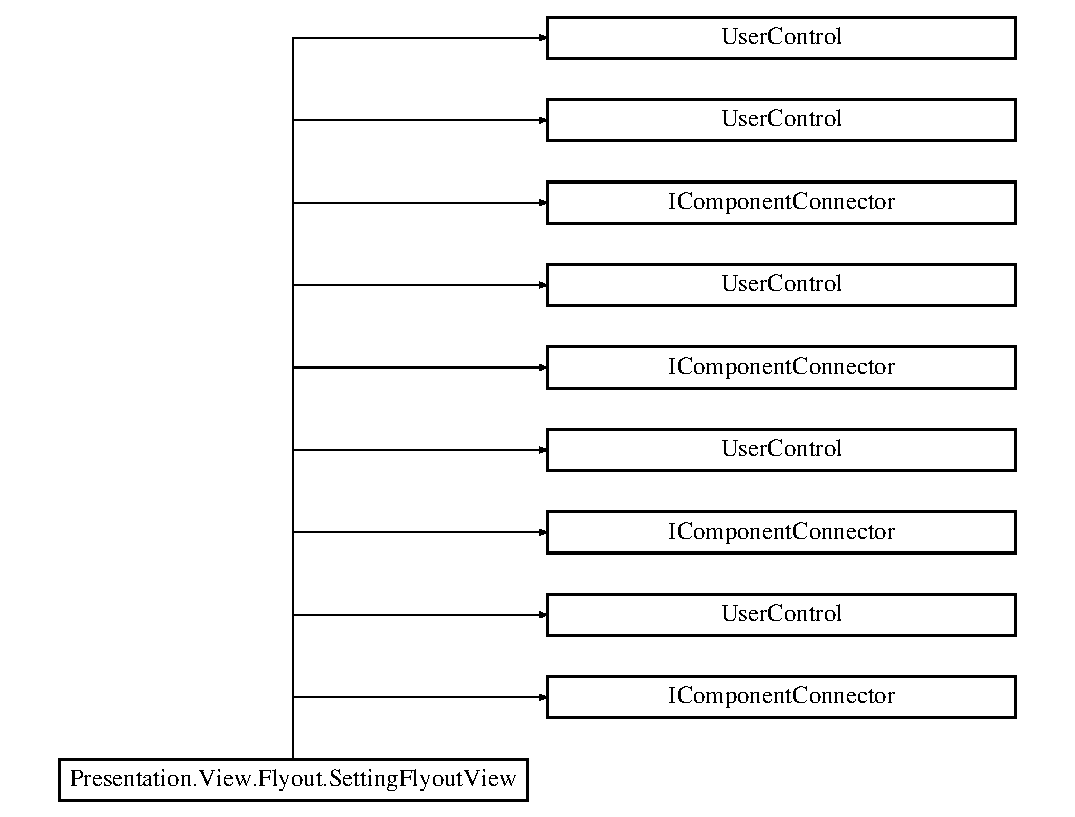
\includegraphics[height=10.000000cm]{class_presentation_1_1_view_1_1_flyout_1_1_setting_flyout_view}
\end{center}
\end{figure}
\subsection*{Public Member Functions}
\begin{DoxyCompactItemize}
\item 
void \hyperlink{class_presentation_1_1_view_1_1_flyout_1_1_setting_flyout_view_abbcaa47b8f30638a2b4254afeb72dd33}{Initialize\+Component} ()
\begin{DoxyCompactList}\small\item\em Initialize\+Component \end{DoxyCompactList}\item 
void \hyperlink{class_presentation_1_1_view_1_1_flyout_1_1_setting_flyout_view_abbcaa47b8f30638a2b4254afeb72dd33}{Initialize\+Component} ()
\begin{DoxyCompactList}\small\item\em Initialize\+Component \end{DoxyCompactList}\item 
void \hyperlink{class_presentation_1_1_view_1_1_flyout_1_1_setting_flyout_view_abbcaa47b8f30638a2b4254afeb72dd33}{Initialize\+Component} ()
\begin{DoxyCompactList}\small\item\em Initialize\+Component \end{DoxyCompactList}\item 
void \hyperlink{class_presentation_1_1_view_1_1_flyout_1_1_setting_flyout_view_abbcaa47b8f30638a2b4254afeb72dd33}{Initialize\+Component} ()
\begin{DoxyCompactList}\small\item\em Initialize\+Component \end{DoxyCompactList}\end{DoxyCompactItemize}


\subsection{Detailed Description}
\hyperlink{class_presentation_1_1_view_1_1_flyout_1_1_setting_flyout_view}{Setting\+Flyout\+View} 

Interaction logic for Setting\+Flyout\+View.\+xaml 

\subsection{Member Function Documentation}
\mbox{\Hypertarget{class_presentation_1_1_view_1_1_flyout_1_1_setting_flyout_view_abbcaa47b8f30638a2b4254afeb72dd33}\label{class_presentation_1_1_view_1_1_flyout_1_1_setting_flyout_view_abbcaa47b8f30638a2b4254afeb72dd33}} 
\index{Presentation\+::\+View\+::\+Flyout\+::\+Setting\+Flyout\+View@{Presentation\+::\+View\+::\+Flyout\+::\+Setting\+Flyout\+View}!Initialize\+Component@{Initialize\+Component}}
\index{Initialize\+Component@{Initialize\+Component}!Presentation\+::\+View\+::\+Flyout\+::\+Setting\+Flyout\+View@{Presentation\+::\+View\+::\+Flyout\+::\+Setting\+Flyout\+View}}
\subsubsection{\texorpdfstring{Initialize\+Component()}{InitializeComponent()}\hspace{0.1cm}{\footnotesize\ttfamily [1/4]}}
{\footnotesize\ttfamily void Presentation.\+View.\+Flyout.\+Setting\+Flyout\+View.\+Initialize\+Component (\begin{DoxyParamCaption}{ }\end{DoxyParamCaption})}



Initialize\+Component 

\mbox{\Hypertarget{class_presentation_1_1_view_1_1_flyout_1_1_setting_flyout_view_abbcaa47b8f30638a2b4254afeb72dd33}\label{class_presentation_1_1_view_1_1_flyout_1_1_setting_flyout_view_abbcaa47b8f30638a2b4254afeb72dd33}} 
\index{Presentation\+::\+View\+::\+Flyout\+::\+Setting\+Flyout\+View@{Presentation\+::\+View\+::\+Flyout\+::\+Setting\+Flyout\+View}!Initialize\+Component@{Initialize\+Component}}
\index{Initialize\+Component@{Initialize\+Component}!Presentation\+::\+View\+::\+Flyout\+::\+Setting\+Flyout\+View@{Presentation\+::\+View\+::\+Flyout\+::\+Setting\+Flyout\+View}}
\subsubsection{\texorpdfstring{Initialize\+Component()}{InitializeComponent()}\hspace{0.1cm}{\footnotesize\ttfamily [2/4]}}
{\footnotesize\ttfamily void Presentation.\+View.\+Flyout.\+Setting\+Flyout\+View.\+Initialize\+Component (\begin{DoxyParamCaption}{ }\end{DoxyParamCaption})}



Initialize\+Component 

\mbox{\Hypertarget{class_presentation_1_1_view_1_1_flyout_1_1_setting_flyout_view_abbcaa47b8f30638a2b4254afeb72dd33}\label{class_presentation_1_1_view_1_1_flyout_1_1_setting_flyout_view_abbcaa47b8f30638a2b4254afeb72dd33}} 
\index{Presentation\+::\+View\+::\+Flyout\+::\+Setting\+Flyout\+View@{Presentation\+::\+View\+::\+Flyout\+::\+Setting\+Flyout\+View}!Initialize\+Component@{Initialize\+Component}}
\index{Initialize\+Component@{Initialize\+Component}!Presentation\+::\+View\+::\+Flyout\+::\+Setting\+Flyout\+View@{Presentation\+::\+View\+::\+Flyout\+::\+Setting\+Flyout\+View}}
\subsubsection{\texorpdfstring{Initialize\+Component()}{InitializeComponent()}\hspace{0.1cm}{\footnotesize\ttfamily [3/4]}}
{\footnotesize\ttfamily void Presentation.\+View.\+Flyout.\+Setting\+Flyout\+View.\+Initialize\+Component (\begin{DoxyParamCaption}{ }\end{DoxyParamCaption})}



Initialize\+Component 

\mbox{\Hypertarget{class_presentation_1_1_view_1_1_flyout_1_1_setting_flyout_view_abbcaa47b8f30638a2b4254afeb72dd33}\label{class_presentation_1_1_view_1_1_flyout_1_1_setting_flyout_view_abbcaa47b8f30638a2b4254afeb72dd33}} 
\index{Presentation\+::\+View\+::\+Flyout\+::\+Setting\+Flyout\+View@{Presentation\+::\+View\+::\+Flyout\+::\+Setting\+Flyout\+View}!Initialize\+Component@{Initialize\+Component}}
\index{Initialize\+Component@{Initialize\+Component}!Presentation\+::\+View\+::\+Flyout\+::\+Setting\+Flyout\+View@{Presentation\+::\+View\+::\+Flyout\+::\+Setting\+Flyout\+View}}
\subsubsection{\texorpdfstring{Initialize\+Component()}{InitializeComponent()}\hspace{0.1cm}{\footnotesize\ttfamily [4/4]}}
{\footnotesize\ttfamily void Presentation.\+View.\+Flyout.\+Setting\+Flyout\+View.\+Initialize\+Component (\begin{DoxyParamCaption}{ }\end{DoxyParamCaption})}



Initialize\+Component 



The documentation for this class was generated from the following files\+:\begin{DoxyCompactItemize}
\item 
C\+:/\+W\+O\+R\+K\+S\+P\+A\+C\+E/\+T\+P\+I-\/end/\+Gestion\+Audio/\+Gestion\+Audio/obj/\+Debug/\+View/\+Flyout/Setting\+Flyout\+View.\+g.\+cs\item 
C\+:/\+W\+O\+R\+K\+S\+P\+A\+C\+E/\+T\+P\+I-\/end/\+Gestion\+Audio/\+Gestion\+Audio/obj/\+Debug/\+View/\+Flyout/Setting\+Flyout\+View.\+g.\+i.\+cs\item 
C\+:/\+W\+O\+R\+K\+S\+P\+A\+C\+E/\+T\+P\+I-\/end/\+Gestion\+Audio/\+Gestion\+Audio/\+View/\+Flyout/Setting\+Flyout\+View.\+xaml.\+cs\end{DoxyCompactItemize}

\hypertarget{class_presentation_1_1_view_model_1_1_setting_flyout_view_model}{}\section{Presentation.\+View\+Model.\+Setting\+Flyout\+View\+Model Class Reference}
\label{class_presentation_1_1_view_model_1_1_setting_flyout_view_model}\index{Presentation.\+View\+Model.\+Setting\+Flyout\+View\+Model@{Presentation.\+View\+Model.\+Setting\+Flyout\+View\+Model}}


This class contain the logic for the setting flyout  


Inheritance diagram for Presentation.\+View\+Model.\+Setting\+Flyout\+View\+Model\+:\begin{figure}[H]
\begin{center}
\leavevmode
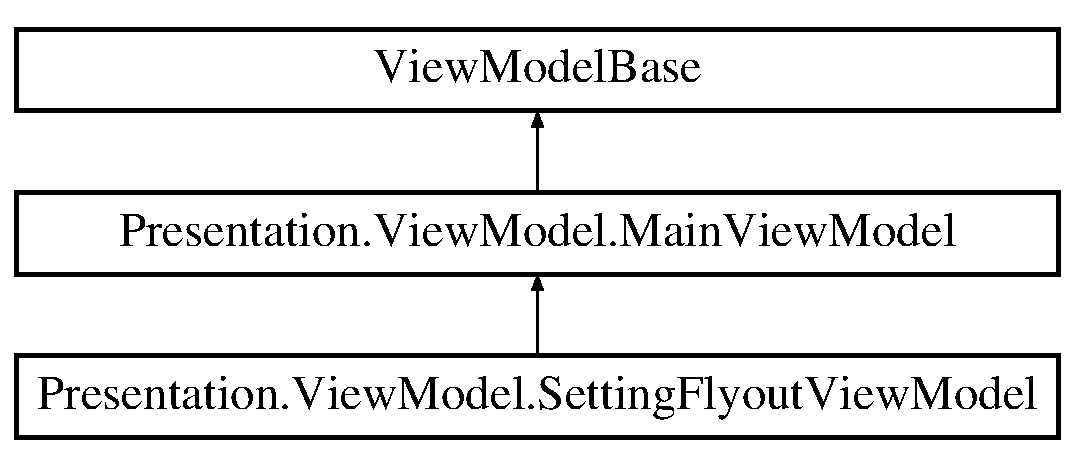
\includegraphics[height=3.000000cm]{class_presentation_1_1_view_model_1_1_setting_flyout_view_model}
\end{center}
\end{figure}
\subsection*{Public Member Functions}
\begin{DoxyCompactItemize}
\item 
\hyperlink{class_presentation_1_1_view_model_1_1_setting_flyout_view_model_a7d2643acc0a988f6b6d5435a2e30b545}{Setting\+Flyout\+View\+Model} ()
\begin{DoxyCompactList}\small\item\em init Relay\+Command \end{DoxyCompactList}\item 
void \hyperlink{class_presentation_1_1_view_model_1_1_setting_flyout_view_model_a380acb37c0bc2c581fda502115e5bc50}{Click\+Add\+Folder} ()
\begin{DoxyCompactList}\small\item\em launch the folder picker to get a folder \end{DoxyCompactList}\item 
\mbox{\Hypertarget{class_presentation_1_1_view_model_1_1_setting_flyout_view_model_adef39f08b4c7a39ffdda5a9d8517032a}\label{class_presentation_1_1_view_model_1_1_setting_flyout_view_model_adef39f08b4c7a39ffdda5a9d8517032a}} 
void \hyperlink{class_presentation_1_1_view_model_1_1_setting_flyout_view_model_adef39f08b4c7a39ffdda5a9d8517032a}{Click\+Remove\+Folder} ()
\begin{DoxyCompactList}\small\item\em remove the selected folder from the list /summary$>$ \end{DoxyCompactList}\item 
void \hyperlink{class_presentation_1_1_view_model_1_1_setting_flyout_view_model_aa4f9ea5fec87225339cfe33d1b8f064d}{Click\+Sync} ()
\begin{DoxyCompactList}\small\item\em Launch a sync \end{DoxyCompactList}\end{DoxyCompactItemize}
\subsection*{Properties}
\begin{DoxyCompactItemize}
\item 
\mbox{\Hypertarget{class_presentation_1_1_view_model_1_1_setting_flyout_view_model_a663ffc6aa12a960caccb8e907a45eb24}\label{class_presentation_1_1_view_model_1_1_setting_flyout_view_model_a663ffc6aa12a960caccb8e907a45eb24}} 
Observable\+Collection$<$ \hyperlink{class_d_t_o_1_1_entity_1_1_include_folder}{Include\+Folder} $>$ {\bfseries Include\+Folders}\hspace{0.3cm}{\ttfamily  \mbox{[}get, set\mbox{]}}
\item 
\mbox{\Hypertarget{class_presentation_1_1_view_model_1_1_setting_flyout_view_model_a26685059dae48243b312b4836c813ce6}\label{class_presentation_1_1_view_model_1_1_setting_flyout_view_model_a26685059dae48243b312b4836c813ce6}} 
bool {\bfseries Launch\+Music\+On\+Start}\hspace{0.3cm}{\ttfamily  \mbox{[}get, set\mbox{]}}
\item 
\mbox{\Hypertarget{class_presentation_1_1_view_model_1_1_setting_flyout_view_model_adc95aa82cc84dc98861051e2bc224aec}\label{class_presentation_1_1_view_model_1_1_setting_flyout_view_model_adc95aa82cc84dc98861051e2bc224aec}} 
Relay\+Command {\bfseries On\+Click\+Add\+Folder}\hspace{0.3cm}{\ttfamily  \mbox{[}get, set\mbox{]}}
\item 
\mbox{\Hypertarget{class_presentation_1_1_view_model_1_1_setting_flyout_view_model_a25c2557764147d7a8ed2f52c011ab08f}\label{class_presentation_1_1_view_model_1_1_setting_flyout_view_model_a25c2557764147d7a8ed2f52c011ab08f}} 
Relay\+Command {\bfseries On\+Click\+Remove\+Folder}\hspace{0.3cm}{\ttfamily  \mbox{[}get, set\mbox{]}}
\item 
\mbox{\Hypertarget{class_presentation_1_1_view_model_1_1_setting_flyout_view_model_a44e44c5b52ddafcb592b05241499449a}\label{class_presentation_1_1_view_model_1_1_setting_flyout_view_model_a44e44c5b52ddafcb592b05241499449a}} 
Relay\+Command {\bfseries On\+Click\+Sync}\hspace{0.3cm}{\ttfamily  \mbox{[}get, set\mbox{]}}
\item 
\mbox{\Hypertarget{class_presentation_1_1_view_model_1_1_setting_flyout_view_model_a3928d6f2d8b2570d9b21de4f2b3e9fdd}\label{class_presentation_1_1_view_model_1_1_setting_flyout_view_model_a3928d6f2d8b2570d9b21de4f2b3e9fdd}} 
\hyperlink{class_d_t_o_1_1_entity_1_1_include_folder}{Include\+Folder} {\bfseries Selected\+Item}\hspace{0.3cm}{\ttfamily  \mbox{[}get, set\mbox{]}}
\end{DoxyCompactItemize}


\subsection{Detailed Description}
This class contain the logic for the setting flyout 



\subsection{Constructor \& Destructor Documentation}
\mbox{\Hypertarget{class_presentation_1_1_view_model_1_1_setting_flyout_view_model_a7d2643acc0a988f6b6d5435a2e30b545}\label{class_presentation_1_1_view_model_1_1_setting_flyout_view_model_a7d2643acc0a988f6b6d5435a2e30b545}} 
\index{Presentation\+::\+View\+Model\+::\+Setting\+Flyout\+View\+Model@{Presentation\+::\+View\+Model\+::\+Setting\+Flyout\+View\+Model}!Setting\+Flyout\+View\+Model@{Setting\+Flyout\+View\+Model}}
\index{Setting\+Flyout\+View\+Model@{Setting\+Flyout\+View\+Model}!Presentation\+::\+View\+Model\+::\+Setting\+Flyout\+View\+Model@{Presentation\+::\+View\+Model\+::\+Setting\+Flyout\+View\+Model}}
\subsubsection{\texorpdfstring{Setting\+Flyout\+View\+Model()}{SettingFlyoutViewModel()}}
{\footnotesize\ttfamily Presentation.\+View\+Model.\+Setting\+Flyout\+View\+Model.\+Setting\+Flyout\+View\+Model (\begin{DoxyParamCaption}{ }\end{DoxyParamCaption})}



init Relay\+Command 



\subsection{Member Function Documentation}
\mbox{\Hypertarget{class_presentation_1_1_view_model_1_1_setting_flyout_view_model_a380acb37c0bc2c581fda502115e5bc50}\label{class_presentation_1_1_view_model_1_1_setting_flyout_view_model_a380acb37c0bc2c581fda502115e5bc50}} 
\index{Presentation\+::\+View\+Model\+::\+Setting\+Flyout\+View\+Model@{Presentation\+::\+View\+Model\+::\+Setting\+Flyout\+View\+Model}!Click\+Add\+Folder@{Click\+Add\+Folder}}
\index{Click\+Add\+Folder@{Click\+Add\+Folder}!Presentation\+::\+View\+Model\+::\+Setting\+Flyout\+View\+Model@{Presentation\+::\+View\+Model\+::\+Setting\+Flyout\+View\+Model}}
\subsubsection{\texorpdfstring{Click\+Add\+Folder()}{ClickAddFolder()}}
{\footnotesize\ttfamily void Presentation.\+View\+Model.\+Setting\+Flyout\+View\+Model.\+Click\+Add\+Folder (\begin{DoxyParamCaption}{ }\end{DoxyParamCaption})}



launch the folder picker to get a folder 

\mbox{\Hypertarget{class_presentation_1_1_view_model_1_1_setting_flyout_view_model_aa4f9ea5fec87225339cfe33d1b8f064d}\label{class_presentation_1_1_view_model_1_1_setting_flyout_view_model_aa4f9ea5fec87225339cfe33d1b8f064d}} 
\index{Presentation\+::\+View\+Model\+::\+Setting\+Flyout\+View\+Model@{Presentation\+::\+View\+Model\+::\+Setting\+Flyout\+View\+Model}!Click\+Sync@{Click\+Sync}}
\index{Click\+Sync@{Click\+Sync}!Presentation\+::\+View\+Model\+::\+Setting\+Flyout\+View\+Model@{Presentation\+::\+View\+Model\+::\+Setting\+Flyout\+View\+Model}}
\subsubsection{\texorpdfstring{Click\+Sync()}{ClickSync()}}
{\footnotesize\ttfamily void Presentation.\+View\+Model.\+Setting\+Flyout\+View\+Model.\+Click\+Sync (\begin{DoxyParamCaption}{ }\end{DoxyParamCaption})}



Launch a sync 



The documentation for this class was generated from the following file\+:\begin{DoxyCompactItemize}
\item 
C\+:/\+W\+O\+R\+K\+S\+P\+A\+C\+E/\+T\+P\+I-\/end/\+Gestion\+Audio/\+Gestion\+Audio/\+View\+Model/Setting\+Flyout\+View\+Model.\+cs\end{DoxyCompactItemize}

\hypertarget{class_presentation_1_1_view_1_1_small_player_view}{}\section{Presentation.\+View.\+Small\+Player\+View Class Reference}
\label{class_presentation_1_1_view_1_1_small_player_view}\index{Presentation.\+View.\+Small\+Player\+View@{Presentation.\+View.\+Small\+Player\+View}}


\hyperlink{class_presentation_1_1_view_1_1_small_player_view}{Small\+Player\+View}  


Inheritance diagram for Presentation.\+View.\+Small\+Player\+View\+:\begin{figure}[H]
\begin{center}
\leavevmode
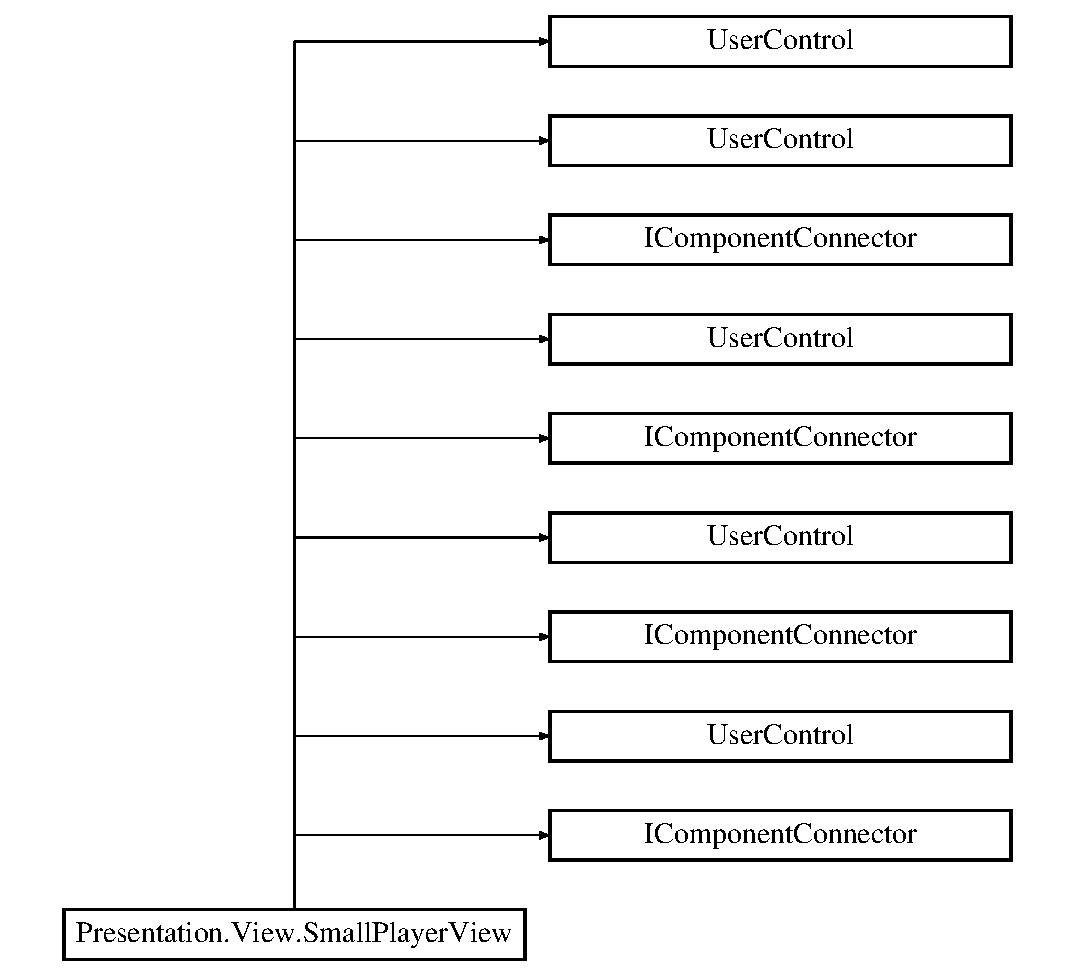
\includegraphics[height=10.000000cm]{class_presentation_1_1_view_1_1_small_player_view}
\end{center}
\end{figure}
\subsection*{Public Member Functions}
\begin{DoxyCompactItemize}
\item 
void \hyperlink{class_presentation_1_1_view_1_1_small_player_view_a1199bc28ab3753d6689a2aaa87142c09}{Initialize\+Component} ()
\begin{DoxyCompactList}\small\item\em Initialize\+Component \end{DoxyCompactList}\item 
void \hyperlink{class_presentation_1_1_view_1_1_small_player_view_a1199bc28ab3753d6689a2aaa87142c09}{Initialize\+Component} ()
\begin{DoxyCompactList}\small\item\em Initialize\+Component \end{DoxyCompactList}\item 
void \hyperlink{class_presentation_1_1_view_1_1_small_player_view_a1199bc28ab3753d6689a2aaa87142c09}{Initialize\+Component} ()
\begin{DoxyCompactList}\small\item\em Initialize\+Component \end{DoxyCompactList}\item 
void \hyperlink{class_presentation_1_1_view_1_1_small_player_view_a1199bc28ab3753d6689a2aaa87142c09}{Initialize\+Component} ()
\begin{DoxyCompactList}\small\item\em Initialize\+Component \end{DoxyCompactList}\end{DoxyCompactItemize}


\subsection{Detailed Description}
\hyperlink{class_presentation_1_1_view_1_1_small_player_view}{Small\+Player\+View} 

Interaction logic for Running.\+xaml 

\subsection{Member Function Documentation}
\mbox{\Hypertarget{class_presentation_1_1_view_1_1_small_player_view_a1199bc28ab3753d6689a2aaa87142c09}\label{class_presentation_1_1_view_1_1_small_player_view_a1199bc28ab3753d6689a2aaa87142c09}} 
\index{Presentation\+::\+View\+::\+Small\+Player\+View@{Presentation\+::\+View\+::\+Small\+Player\+View}!Initialize\+Component@{Initialize\+Component}}
\index{Initialize\+Component@{Initialize\+Component}!Presentation\+::\+View\+::\+Small\+Player\+View@{Presentation\+::\+View\+::\+Small\+Player\+View}}
\subsubsection{\texorpdfstring{Initialize\+Component()}{InitializeComponent()}\hspace{0.1cm}{\footnotesize\ttfamily [1/4]}}
{\footnotesize\ttfamily void Presentation.\+View.\+Small\+Player\+View.\+Initialize\+Component (\begin{DoxyParamCaption}{ }\end{DoxyParamCaption})}



Initialize\+Component 

\mbox{\Hypertarget{class_presentation_1_1_view_1_1_small_player_view_a1199bc28ab3753d6689a2aaa87142c09}\label{class_presentation_1_1_view_1_1_small_player_view_a1199bc28ab3753d6689a2aaa87142c09}} 
\index{Presentation\+::\+View\+::\+Small\+Player\+View@{Presentation\+::\+View\+::\+Small\+Player\+View}!Initialize\+Component@{Initialize\+Component}}
\index{Initialize\+Component@{Initialize\+Component}!Presentation\+::\+View\+::\+Small\+Player\+View@{Presentation\+::\+View\+::\+Small\+Player\+View}}
\subsubsection{\texorpdfstring{Initialize\+Component()}{InitializeComponent()}\hspace{0.1cm}{\footnotesize\ttfamily [2/4]}}
{\footnotesize\ttfamily void Presentation.\+View.\+Small\+Player\+View.\+Initialize\+Component (\begin{DoxyParamCaption}{ }\end{DoxyParamCaption})}



Initialize\+Component 

\mbox{\Hypertarget{class_presentation_1_1_view_1_1_small_player_view_a1199bc28ab3753d6689a2aaa87142c09}\label{class_presentation_1_1_view_1_1_small_player_view_a1199bc28ab3753d6689a2aaa87142c09}} 
\index{Presentation\+::\+View\+::\+Small\+Player\+View@{Presentation\+::\+View\+::\+Small\+Player\+View}!Initialize\+Component@{Initialize\+Component}}
\index{Initialize\+Component@{Initialize\+Component}!Presentation\+::\+View\+::\+Small\+Player\+View@{Presentation\+::\+View\+::\+Small\+Player\+View}}
\subsubsection{\texorpdfstring{Initialize\+Component()}{InitializeComponent()}\hspace{0.1cm}{\footnotesize\ttfamily [3/4]}}
{\footnotesize\ttfamily void Presentation.\+View.\+Small\+Player\+View.\+Initialize\+Component (\begin{DoxyParamCaption}{ }\end{DoxyParamCaption})}



Initialize\+Component 

\mbox{\Hypertarget{class_presentation_1_1_view_1_1_small_player_view_a1199bc28ab3753d6689a2aaa87142c09}\label{class_presentation_1_1_view_1_1_small_player_view_a1199bc28ab3753d6689a2aaa87142c09}} 
\index{Presentation\+::\+View\+::\+Small\+Player\+View@{Presentation\+::\+View\+::\+Small\+Player\+View}!Initialize\+Component@{Initialize\+Component}}
\index{Initialize\+Component@{Initialize\+Component}!Presentation\+::\+View\+::\+Small\+Player\+View@{Presentation\+::\+View\+::\+Small\+Player\+View}}
\subsubsection{\texorpdfstring{Initialize\+Component()}{InitializeComponent()}\hspace{0.1cm}{\footnotesize\ttfamily [4/4]}}
{\footnotesize\ttfamily void Presentation.\+View.\+Small\+Player\+View.\+Initialize\+Component (\begin{DoxyParamCaption}{ }\end{DoxyParamCaption})}



Initialize\+Component 



The documentation for this class was generated from the following files\+:\begin{DoxyCompactItemize}
\item 
C\+:/\+W\+O\+R\+K\+S\+P\+A\+C\+E/\+T\+P\+I-\/end/\+Gestion\+Audio/\+Gestion\+Audio/obj/\+Debug/\+View/Small\+Player\+View.\+g.\+cs\item 
C\+:/\+W\+O\+R\+K\+S\+P\+A\+C\+E/\+T\+P\+I-\/end/\+Gestion\+Audio/\+Gestion\+Audio/obj/\+Debug/\+View/Small\+Player\+View.\+g.\+i.\+cs\item 
C\+:/\+W\+O\+R\+K\+S\+P\+A\+C\+E/\+T\+P\+I-\/end/\+Gestion\+Audio/\+Gestion\+Audio/\+View/Small\+Player\+View.\+xaml.\+cs\end{DoxyCompactItemize}

\hypertarget{class_d_a_l_1_1_database_1_1_sq_lite_configuration}{}\section{D\+A\+L.\+Database.\+Sq\+Lite\+Configuration Class Reference}
\label{class_d_a_l_1_1_database_1_1_sq_lite_configuration}\index{D\+A\+L.\+Database.\+Sq\+Lite\+Configuration@{D\+A\+L.\+Database.\+Sq\+Lite\+Configuration}}


Settings for sqlite  


Inheritance diagram for D\+A\+L.\+Database.\+Sq\+Lite\+Configuration\+:\begin{figure}[H]
\begin{center}
\leavevmode
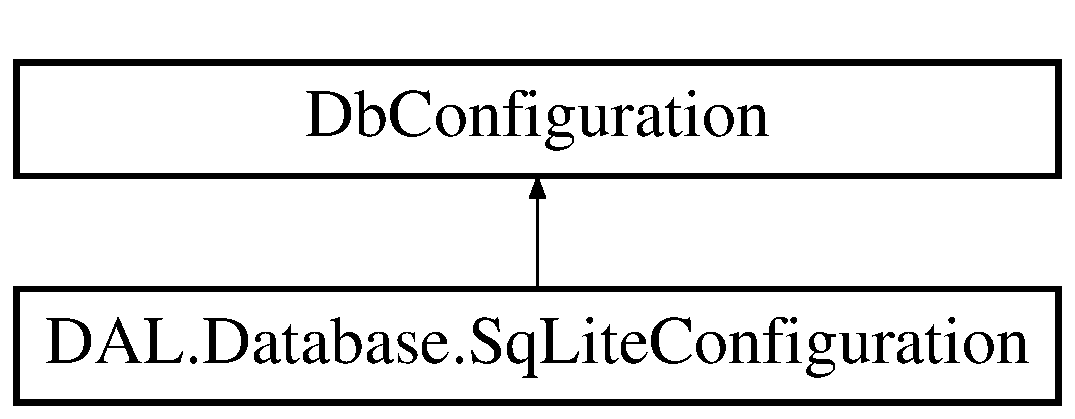
\includegraphics[height=2.000000cm]{class_d_a_l_1_1_database_1_1_sq_lite_configuration}
\end{center}
\end{figure}
\subsection*{Public Member Functions}
\begin{DoxyCompactItemize}
\item 
\hyperlink{class_d_a_l_1_1_database_1_1_sq_lite_configuration_af3159b6c66b120187944bfe862d6acde}{Sq\+Lite\+Configuration} ()
\begin{DoxyCompactList}\small\item\em settings of the provider for S\+Q\+Lite \end{DoxyCompactList}\end{DoxyCompactItemize}


\subsection{Detailed Description}
Settings for sqlite 



\subsection{Constructor \& Destructor Documentation}
\mbox{\Hypertarget{class_d_a_l_1_1_database_1_1_sq_lite_configuration_af3159b6c66b120187944bfe862d6acde}\label{class_d_a_l_1_1_database_1_1_sq_lite_configuration_af3159b6c66b120187944bfe862d6acde}} 
\index{D\+A\+L\+::\+Database\+::\+Sq\+Lite\+Configuration@{D\+A\+L\+::\+Database\+::\+Sq\+Lite\+Configuration}!Sq\+Lite\+Configuration@{Sq\+Lite\+Configuration}}
\index{Sq\+Lite\+Configuration@{Sq\+Lite\+Configuration}!D\+A\+L\+::\+Database\+::\+Sq\+Lite\+Configuration@{D\+A\+L\+::\+Database\+::\+Sq\+Lite\+Configuration}}
\subsubsection{\texorpdfstring{Sq\+Lite\+Configuration()}{SqLiteConfiguration()}}
{\footnotesize\ttfamily D\+A\+L.\+Database.\+Sq\+Lite\+Configuration.\+Sq\+Lite\+Configuration (\begin{DoxyParamCaption}{ }\end{DoxyParamCaption})}



settings of the provider for S\+Q\+Lite 



The documentation for this class was generated from the following file\+:\begin{DoxyCompactItemize}
\item 
C\+:/\+W\+O\+R\+K\+S\+P\+A\+C\+E/\+T\+P\+I-\/end/\+Gestion\+Audio/\+D\+A\+L/\+Database/Configuration.\+cs\end{DoxyCompactItemize}

\hypertarget{class_presentation_1_1_view_1_1_list_1_1_suggest_list_view}{}\section{Presentation.\+View.\+List.\+Suggest\+List\+View Class Reference}
\label{class_presentation_1_1_view_1_1_list_1_1_suggest_list_view}\index{Presentation.\+View.\+List.\+Suggest\+List\+View@{Presentation.\+View.\+List.\+Suggest\+List\+View}}


\hyperlink{class_presentation_1_1_view_1_1_list_1_1_suggest_list_view}{Suggest\+List\+View}  


Inheritance diagram for Presentation.\+View.\+List.\+Suggest\+List\+View\+:\begin{figure}[H]
\begin{center}
\leavevmode
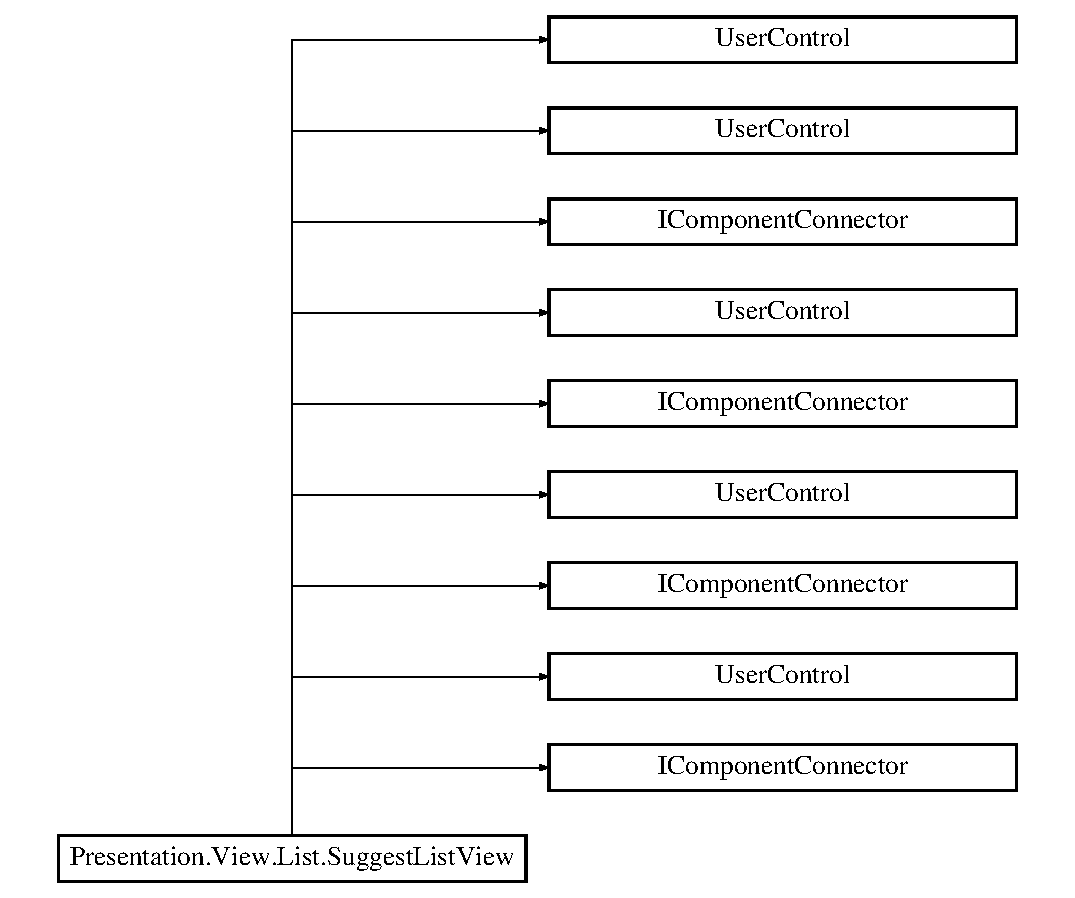
\includegraphics[height=10.000000cm]{class_presentation_1_1_view_1_1_list_1_1_suggest_list_view}
\end{center}
\end{figure}
\subsection*{Public Member Functions}
\begin{DoxyCompactItemize}
\item 
void \hyperlink{class_presentation_1_1_view_1_1_list_1_1_suggest_list_view_a0d6458960ea2444bee0d02317d0f2baa}{Initialize\+Component} ()
\begin{DoxyCompactList}\small\item\em Initialize\+Component \end{DoxyCompactList}\item 
void \hyperlink{class_presentation_1_1_view_1_1_list_1_1_suggest_list_view_a0d6458960ea2444bee0d02317d0f2baa}{Initialize\+Component} ()
\begin{DoxyCompactList}\small\item\em Initialize\+Component \end{DoxyCompactList}\item 
void \hyperlink{class_presentation_1_1_view_1_1_list_1_1_suggest_list_view_a0d6458960ea2444bee0d02317d0f2baa}{Initialize\+Component} ()
\begin{DoxyCompactList}\small\item\em Initialize\+Component \end{DoxyCompactList}\item 
void \hyperlink{class_presentation_1_1_view_1_1_list_1_1_suggest_list_view_a0d6458960ea2444bee0d02317d0f2baa}{Initialize\+Component} ()
\begin{DoxyCompactList}\small\item\em Initialize\+Component \end{DoxyCompactList}\end{DoxyCompactItemize}


\subsection{Detailed Description}
\hyperlink{class_presentation_1_1_view_1_1_list_1_1_suggest_list_view}{Suggest\+List\+View} 

Interaction logic for Music\+Home.\+xaml 

\subsection{Member Function Documentation}
\mbox{\Hypertarget{class_presentation_1_1_view_1_1_list_1_1_suggest_list_view_a0d6458960ea2444bee0d02317d0f2baa}\label{class_presentation_1_1_view_1_1_list_1_1_suggest_list_view_a0d6458960ea2444bee0d02317d0f2baa}} 
\index{Presentation\+::\+View\+::\+List\+::\+Suggest\+List\+View@{Presentation\+::\+View\+::\+List\+::\+Suggest\+List\+View}!Initialize\+Component@{Initialize\+Component}}
\index{Initialize\+Component@{Initialize\+Component}!Presentation\+::\+View\+::\+List\+::\+Suggest\+List\+View@{Presentation\+::\+View\+::\+List\+::\+Suggest\+List\+View}}
\subsubsection{\texorpdfstring{Initialize\+Component()}{InitializeComponent()}\hspace{0.1cm}{\footnotesize\ttfamily [1/4]}}
{\footnotesize\ttfamily void Presentation.\+View.\+List.\+Suggest\+List\+View.\+Initialize\+Component (\begin{DoxyParamCaption}{ }\end{DoxyParamCaption})}



Initialize\+Component 

\mbox{\Hypertarget{class_presentation_1_1_view_1_1_list_1_1_suggest_list_view_a0d6458960ea2444bee0d02317d0f2baa}\label{class_presentation_1_1_view_1_1_list_1_1_suggest_list_view_a0d6458960ea2444bee0d02317d0f2baa}} 
\index{Presentation\+::\+View\+::\+List\+::\+Suggest\+List\+View@{Presentation\+::\+View\+::\+List\+::\+Suggest\+List\+View}!Initialize\+Component@{Initialize\+Component}}
\index{Initialize\+Component@{Initialize\+Component}!Presentation\+::\+View\+::\+List\+::\+Suggest\+List\+View@{Presentation\+::\+View\+::\+List\+::\+Suggest\+List\+View}}
\subsubsection{\texorpdfstring{Initialize\+Component()}{InitializeComponent()}\hspace{0.1cm}{\footnotesize\ttfamily [2/4]}}
{\footnotesize\ttfamily void Presentation.\+View.\+List.\+Suggest\+List\+View.\+Initialize\+Component (\begin{DoxyParamCaption}{ }\end{DoxyParamCaption})}



Initialize\+Component 

\mbox{\Hypertarget{class_presentation_1_1_view_1_1_list_1_1_suggest_list_view_a0d6458960ea2444bee0d02317d0f2baa}\label{class_presentation_1_1_view_1_1_list_1_1_suggest_list_view_a0d6458960ea2444bee0d02317d0f2baa}} 
\index{Presentation\+::\+View\+::\+List\+::\+Suggest\+List\+View@{Presentation\+::\+View\+::\+List\+::\+Suggest\+List\+View}!Initialize\+Component@{Initialize\+Component}}
\index{Initialize\+Component@{Initialize\+Component}!Presentation\+::\+View\+::\+List\+::\+Suggest\+List\+View@{Presentation\+::\+View\+::\+List\+::\+Suggest\+List\+View}}
\subsubsection{\texorpdfstring{Initialize\+Component()}{InitializeComponent()}\hspace{0.1cm}{\footnotesize\ttfamily [3/4]}}
{\footnotesize\ttfamily void Presentation.\+View.\+List.\+Suggest\+List\+View.\+Initialize\+Component (\begin{DoxyParamCaption}{ }\end{DoxyParamCaption})}



Initialize\+Component 

\mbox{\Hypertarget{class_presentation_1_1_view_1_1_list_1_1_suggest_list_view_a0d6458960ea2444bee0d02317d0f2baa}\label{class_presentation_1_1_view_1_1_list_1_1_suggest_list_view_a0d6458960ea2444bee0d02317d0f2baa}} 
\index{Presentation\+::\+View\+::\+List\+::\+Suggest\+List\+View@{Presentation\+::\+View\+::\+List\+::\+Suggest\+List\+View}!Initialize\+Component@{Initialize\+Component}}
\index{Initialize\+Component@{Initialize\+Component}!Presentation\+::\+View\+::\+List\+::\+Suggest\+List\+View@{Presentation\+::\+View\+::\+List\+::\+Suggest\+List\+View}}
\subsubsection{\texorpdfstring{Initialize\+Component()}{InitializeComponent()}\hspace{0.1cm}{\footnotesize\ttfamily [4/4]}}
{\footnotesize\ttfamily void Presentation.\+View.\+List.\+Suggest\+List\+View.\+Initialize\+Component (\begin{DoxyParamCaption}{ }\end{DoxyParamCaption})}



Initialize\+Component 



The documentation for this class was generated from the following files\+:\begin{DoxyCompactItemize}
\item 
C\+:/\+W\+O\+R\+K\+S\+P\+A\+C\+E/\+T\+P\+I-\/end/\+Gestion\+Audio/\+Gestion\+Audio/obj/\+Debug/\+View/\+List/Suggest\+List\+View.\+g.\+cs\item 
C\+:/\+W\+O\+R\+K\+S\+P\+A\+C\+E/\+T\+P\+I-\/end/\+Gestion\+Audio/\+Gestion\+Audio/obj/\+Debug/\+View/\+List/Suggest\+List\+View.\+g.\+i.\+cs\item 
C\+:/\+W\+O\+R\+K\+S\+P\+A\+C\+E/\+T\+P\+I-\/end/\+Gestion\+Audio/\+Gestion\+Audio/\+View/\+List/Suggest\+List\+View.\+xaml.\+cs\end{DoxyCompactItemize}

\hypertarget{class_unit_test_1_1_sync_test}{}\section{Unit\+Test.\+Sync\+Test Class Reference}
\label{class_unit_test_1_1_sync_test}\index{Unit\+Test.\+Sync\+Test@{Unit\+Test.\+Sync\+Test}}


Contain all test to make the sync  


\subsection*{Public Member Functions}
\begin{DoxyCompactItemize}
\item 
void \hyperlink{class_unit_test_1_1_sync_test_a0a50b296418fd090f3d1fa085a328ab8}{Analyse\+Folder\+Tree} ()
\begin{DoxyCompactList}\small\item\em check that folder are the folders I was looking for \end{DoxyCompactList}\item 
void \hyperlink{class_unit_test_1_1_sync_test_a988e686b462be304ca52e67b9f1876a3}{Sync\+Folder} ()
\begin{DoxyCompactList}\small\item\em Try to sync a folder with the database \end{DoxyCompactList}\end{DoxyCompactItemize}


\subsection{Detailed Description}
Contain all test to make the sync 



\subsection{Member Function Documentation}
\mbox{\Hypertarget{class_unit_test_1_1_sync_test_a0a50b296418fd090f3d1fa085a328ab8}\label{class_unit_test_1_1_sync_test_a0a50b296418fd090f3d1fa085a328ab8}} 
\index{Unit\+Test\+::\+Sync\+Test@{Unit\+Test\+::\+Sync\+Test}!Analyse\+Folder\+Tree@{Analyse\+Folder\+Tree}}
\index{Analyse\+Folder\+Tree@{Analyse\+Folder\+Tree}!Unit\+Test\+::\+Sync\+Test@{Unit\+Test\+::\+Sync\+Test}}
\subsubsection{\texorpdfstring{Analyse\+Folder\+Tree()}{AnalyseFolderTree()}}
{\footnotesize\ttfamily void Unit\+Test.\+Sync\+Test.\+Analyse\+Folder\+Tree (\begin{DoxyParamCaption}{ }\end{DoxyParamCaption})}



check that folder are the folders I was looking for 

\mbox{\Hypertarget{class_unit_test_1_1_sync_test_a988e686b462be304ca52e67b9f1876a3}\label{class_unit_test_1_1_sync_test_a988e686b462be304ca52e67b9f1876a3}} 
\index{Unit\+Test\+::\+Sync\+Test@{Unit\+Test\+::\+Sync\+Test}!Sync\+Folder@{Sync\+Folder}}
\index{Sync\+Folder@{Sync\+Folder}!Unit\+Test\+::\+Sync\+Test@{Unit\+Test\+::\+Sync\+Test}}
\subsubsection{\texorpdfstring{Sync\+Folder()}{SyncFolder()}}
{\footnotesize\ttfamily void Unit\+Test.\+Sync\+Test.\+Sync\+Folder (\begin{DoxyParamCaption}{ }\end{DoxyParamCaption})}



Try to sync a folder with the database 



The documentation for this class was generated from the following file\+:\begin{DoxyCompactItemize}
\item 
C\+:/\+W\+O\+R\+K\+S\+P\+A\+C\+E/\+T\+P\+I-\/end/\+Gestion\+Audio/\+Unit\+Test/Sync\+Test.\+cs\end{DoxyCompactItemize}

\hypertarget{class_d_t_o_1_1_entity_1_1_track}{}\section{D\+T\+O.\+Entity.\+Track Class Reference}
\label{class_d_t_o_1_1_entity_1_1_track}\index{D\+T\+O.\+Entity.\+Track@{D\+T\+O.\+Entity.\+Track}}


The database \hyperlink{class_d_t_o_1_1_entity_1_1_track}{Track} entity  


Inheritance diagram for D\+T\+O.\+Entity.\+Track\+:\begin{figure}[H]
\begin{center}
\leavevmode
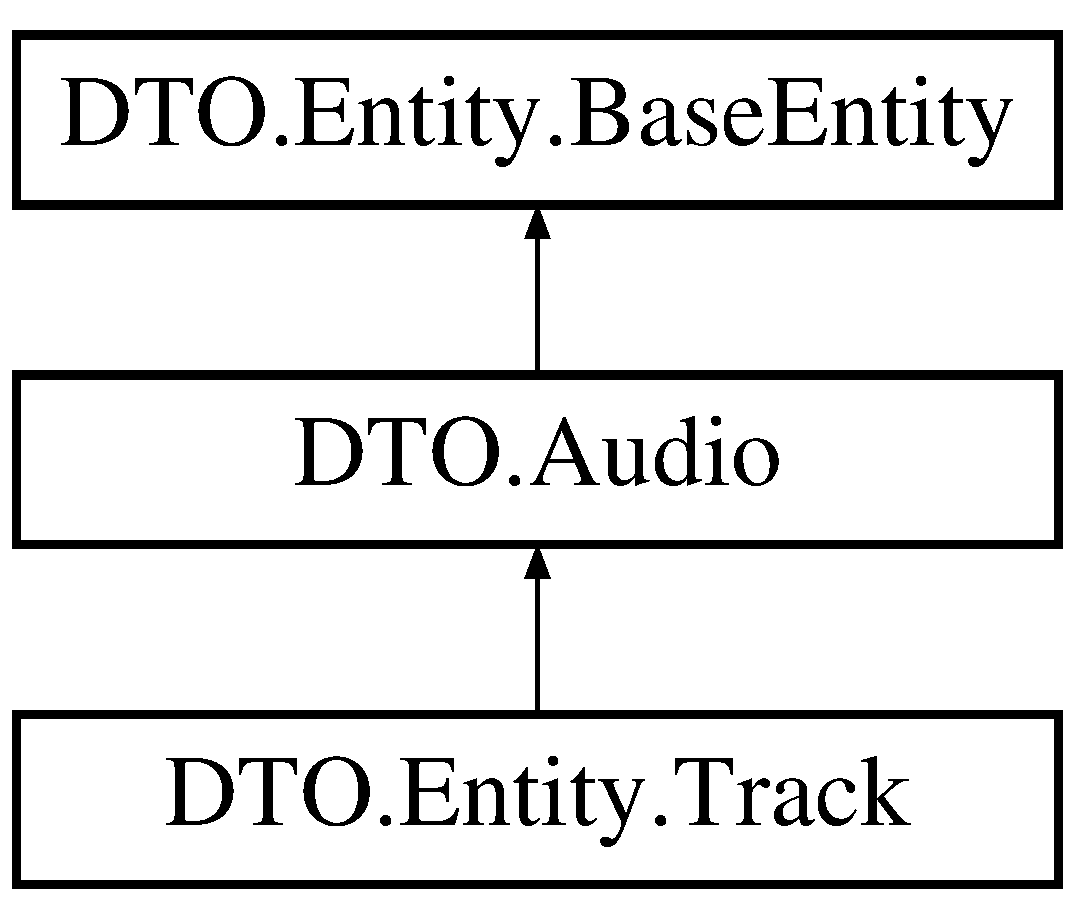
\includegraphics[height=3.000000cm]{class_d_t_o_1_1_entity_1_1_track}
\end{center}
\end{figure}
\subsection*{Public Attributes}
\begin{DoxyCompactItemize}
\item 
\mbox{\Hypertarget{class_d_t_o_1_1_entity_1_1_track_a9d78da85a455dfc89c12398a23a66877}\label{class_d_t_o_1_1_entity_1_1_track_a9d78da85a455dfc89c12398a23a66877}} 
Time\+Span {\bfseries Duration\+Time} =$>$ Time\+Span.\+From\+Milliseconds(Duration)
\end{DoxyCompactItemize}
\subsection*{Properties}
\begin{DoxyCompactItemize}
\item 
\mbox{\Hypertarget{class_d_t_o_1_1_entity_1_1_track_a8798ee8fe10a9f530a6bfe9f009c9bf4}\label{class_d_t_o_1_1_entity_1_1_track_a8798ee8fe10a9f530a6bfe9f009c9bf4}} 
virtual \hyperlink{class_d_t_o_1_1_entity_1_1_album}{Album} {\bfseries Album}\hspace{0.3cm}{\ttfamily  \mbox{[}get, set\mbox{]}}
\item 
\mbox{\Hypertarget{class_d_t_o_1_1_entity_1_1_track_a23c46b08fc20d064666238ac7b677878}\label{class_d_t_o_1_1_entity_1_1_track_a23c46b08fc20d064666238ac7b677878}} 
int {\bfseries Duration}\hspace{0.3cm}{\ttfamily  \mbox{[}get, set\mbox{]}}
\item 
\mbox{\Hypertarget{class_d_t_o_1_1_entity_1_1_track_a4972041acdc42377b1550e029d50da10}\label{class_d_t_o_1_1_entity_1_1_track_a4972041acdc42377b1550e029d50da10}} 
long {\bfseries fk\+Album}\hspace{0.3cm}{\ttfamily  \mbox{[}get, set\mbox{]}}
\item 
\mbox{\Hypertarget{class_d_t_o_1_1_entity_1_1_track_a22ac890cc5e17003daba71051a39e33b}\label{class_d_t_o_1_1_entity_1_1_track_a22ac890cc5e17003daba71051a39e33b}} 
int {\bfseries Listened\+Times}\hspace{0.3cm}{\ttfamily  \mbox{[}get, set\mbox{]}}
\item 
\mbox{\Hypertarget{class_d_t_o_1_1_entity_1_1_track_a14587bea688f9cd330b9857315a5c5cf}\label{class_d_t_o_1_1_entity_1_1_track_a14587bea688f9cd330b9857315a5c5cf}} 
virtual List$<$ \hyperlink{class_d_t_o_1_1_entity_1_1_playlist}{Playlist} $>$ {\bfseries Playlists}\hspace{0.3cm}{\ttfamily  \mbox{[}get, set\mbox{]}}
\end{DoxyCompactItemize}


\subsection{Detailed Description}
The database \hyperlink{class_d_t_o_1_1_entity_1_1_track}{Track} entity 



The documentation for this class was generated from the following file\+:\begin{DoxyCompactItemize}
\item 
C\+:/\+W\+O\+R\+K\+S\+P\+A\+C\+E/\+T\+P\+I-\/end/\+Gestion\+Audio/\+D\+T\+O/\+Entity/Track.\+cs\end{DoxyCompactItemize}

\hypertarget{class_presentation_1_1_view_1_1_list_1_1_track_list_view}{}\section{Presentation.\+View.\+List.\+Track\+List\+View Class Reference}
\label{class_presentation_1_1_view_1_1_list_1_1_track_list_view}\index{Presentation.\+View.\+List.\+Track\+List\+View@{Presentation.\+View.\+List.\+Track\+List\+View}}


\hyperlink{class_presentation_1_1_view_1_1_list_1_1_track_list_view}{Track\+List\+View}  


Inheritance diagram for Presentation.\+View.\+List.\+Track\+List\+View\+:\begin{figure}[H]
\begin{center}
\leavevmode
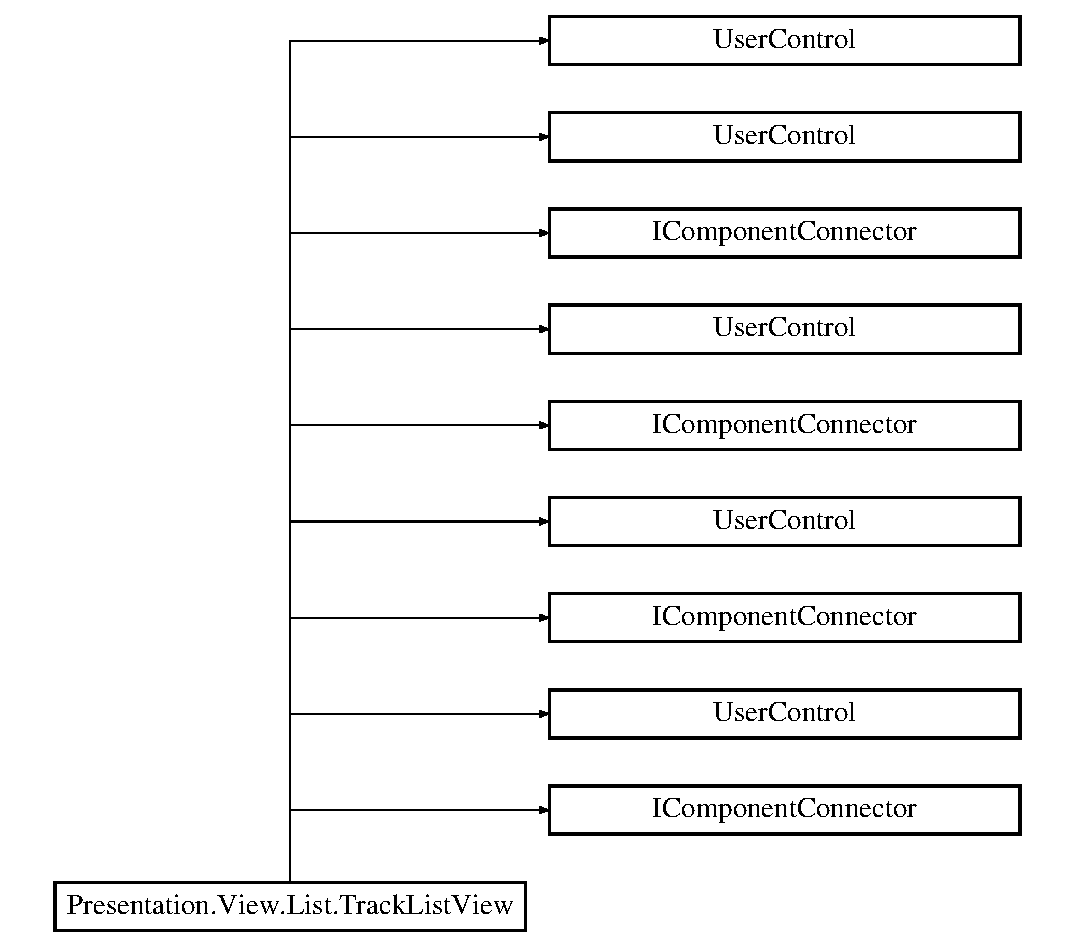
\includegraphics[height=10.000000cm]{class_presentation_1_1_view_1_1_list_1_1_track_list_view}
\end{center}
\end{figure}
\subsection*{Public Member Functions}
\begin{DoxyCompactItemize}
\item 
void \hyperlink{class_presentation_1_1_view_1_1_list_1_1_track_list_view_a86e2e69667d5d62053af1e28d00daaee}{Initialize\+Component} ()
\begin{DoxyCompactList}\small\item\em Initialize\+Component \end{DoxyCompactList}\item 
void \hyperlink{class_presentation_1_1_view_1_1_list_1_1_track_list_view_a86e2e69667d5d62053af1e28d00daaee}{Initialize\+Component} ()
\begin{DoxyCompactList}\small\item\em Initialize\+Component \end{DoxyCompactList}\item 
void \hyperlink{class_presentation_1_1_view_1_1_list_1_1_track_list_view_a86e2e69667d5d62053af1e28d00daaee}{Initialize\+Component} ()
\begin{DoxyCompactList}\small\item\em Initialize\+Component \end{DoxyCompactList}\item 
void \hyperlink{class_presentation_1_1_view_1_1_list_1_1_track_list_view_a86e2e69667d5d62053af1e28d00daaee}{Initialize\+Component} ()
\begin{DoxyCompactList}\small\item\em Initialize\+Component \end{DoxyCompactList}\end{DoxyCompactItemize}


\subsection{Detailed Description}
\hyperlink{class_presentation_1_1_view_1_1_list_1_1_track_list_view}{Track\+List\+View} 

Interaction logic for Music\+Home.\+xaml 

\subsection{Member Function Documentation}
\mbox{\Hypertarget{class_presentation_1_1_view_1_1_list_1_1_track_list_view_a86e2e69667d5d62053af1e28d00daaee}\label{class_presentation_1_1_view_1_1_list_1_1_track_list_view_a86e2e69667d5d62053af1e28d00daaee}} 
\index{Presentation\+::\+View\+::\+List\+::\+Track\+List\+View@{Presentation\+::\+View\+::\+List\+::\+Track\+List\+View}!Initialize\+Component@{Initialize\+Component}}
\index{Initialize\+Component@{Initialize\+Component}!Presentation\+::\+View\+::\+List\+::\+Track\+List\+View@{Presentation\+::\+View\+::\+List\+::\+Track\+List\+View}}
\subsubsection{\texorpdfstring{Initialize\+Component()}{InitializeComponent()}\hspace{0.1cm}{\footnotesize\ttfamily [1/4]}}
{\footnotesize\ttfamily void Presentation.\+View.\+List.\+Track\+List\+View.\+Initialize\+Component (\begin{DoxyParamCaption}{ }\end{DoxyParamCaption})}



Initialize\+Component 

\mbox{\Hypertarget{class_presentation_1_1_view_1_1_list_1_1_track_list_view_a86e2e69667d5d62053af1e28d00daaee}\label{class_presentation_1_1_view_1_1_list_1_1_track_list_view_a86e2e69667d5d62053af1e28d00daaee}} 
\index{Presentation\+::\+View\+::\+List\+::\+Track\+List\+View@{Presentation\+::\+View\+::\+List\+::\+Track\+List\+View}!Initialize\+Component@{Initialize\+Component}}
\index{Initialize\+Component@{Initialize\+Component}!Presentation\+::\+View\+::\+List\+::\+Track\+List\+View@{Presentation\+::\+View\+::\+List\+::\+Track\+List\+View}}
\subsubsection{\texorpdfstring{Initialize\+Component()}{InitializeComponent()}\hspace{0.1cm}{\footnotesize\ttfamily [2/4]}}
{\footnotesize\ttfamily void Presentation.\+View.\+List.\+Track\+List\+View.\+Initialize\+Component (\begin{DoxyParamCaption}{ }\end{DoxyParamCaption})}



Initialize\+Component 

\mbox{\Hypertarget{class_presentation_1_1_view_1_1_list_1_1_track_list_view_a86e2e69667d5d62053af1e28d00daaee}\label{class_presentation_1_1_view_1_1_list_1_1_track_list_view_a86e2e69667d5d62053af1e28d00daaee}} 
\index{Presentation\+::\+View\+::\+List\+::\+Track\+List\+View@{Presentation\+::\+View\+::\+List\+::\+Track\+List\+View}!Initialize\+Component@{Initialize\+Component}}
\index{Initialize\+Component@{Initialize\+Component}!Presentation\+::\+View\+::\+List\+::\+Track\+List\+View@{Presentation\+::\+View\+::\+List\+::\+Track\+List\+View}}
\subsubsection{\texorpdfstring{Initialize\+Component()}{InitializeComponent()}\hspace{0.1cm}{\footnotesize\ttfamily [3/4]}}
{\footnotesize\ttfamily void Presentation.\+View.\+List.\+Track\+List\+View.\+Initialize\+Component (\begin{DoxyParamCaption}{ }\end{DoxyParamCaption})}



Initialize\+Component 

\mbox{\Hypertarget{class_presentation_1_1_view_1_1_list_1_1_track_list_view_a86e2e69667d5d62053af1e28d00daaee}\label{class_presentation_1_1_view_1_1_list_1_1_track_list_view_a86e2e69667d5d62053af1e28d00daaee}} 
\index{Presentation\+::\+View\+::\+List\+::\+Track\+List\+View@{Presentation\+::\+View\+::\+List\+::\+Track\+List\+View}!Initialize\+Component@{Initialize\+Component}}
\index{Initialize\+Component@{Initialize\+Component}!Presentation\+::\+View\+::\+List\+::\+Track\+List\+View@{Presentation\+::\+View\+::\+List\+::\+Track\+List\+View}}
\subsubsection{\texorpdfstring{Initialize\+Component()}{InitializeComponent()}\hspace{0.1cm}{\footnotesize\ttfamily [4/4]}}
{\footnotesize\ttfamily void Presentation.\+View.\+List.\+Track\+List\+View.\+Initialize\+Component (\begin{DoxyParamCaption}{ }\end{DoxyParamCaption})}



Initialize\+Component 



The documentation for this class was generated from the following files\+:\begin{DoxyCompactItemize}
\item 
C\+:/\+W\+O\+R\+K\+S\+P\+A\+C\+E/\+T\+P\+I-\/end/\+Gestion\+Audio/\+Gestion\+Audio/obj/\+Debug/\+View/\+List/Track\+List\+View.\+g.\+cs\item 
C\+:/\+W\+O\+R\+K\+S\+P\+A\+C\+E/\+T\+P\+I-\/end/\+Gestion\+Audio/\+Gestion\+Audio/obj/\+Debug/\+View/\+List/Track\+List\+View.\+g.\+i.\+cs\item 
C\+:/\+W\+O\+R\+K\+S\+P\+A\+C\+E/\+T\+P\+I-\/end/\+Gestion\+Audio/\+Gestion\+Audio/\+View/\+List/Track\+List\+View.\+xaml.\+cs\end{DoxyCompactItemize}

%--- End generated contents ---

% Index
\backmatter
\newpage
\phantomsection
\clearemptydoublepage
\addcontentsline{toc}{chapter}{Index}
\printindex

\end{document}
